\documentclass{ucdthesis}       % Final

% Code Generation Packages
\usepackage{pseudocode}
\newcommand{\proc}[1]{\ensuremath{\CALL{#1}}}
\newcommand{\func}[2]{\CALL{#1}{#2}}
\newcommand{\meth}{\negthickspace \rightarrow \negthickspace}
%\newcommand{\meth}{\negmedspace \centerdot}
%\newcommand{\meth}{.}
\newcommand{\METH}[2]{\meth\CALL{#1}{#2}}

% geostreams have common drawing stuff.
\usepackage{geostreams}
\usepackage{array}
\usepackage{xr}
\usepackage{epsfig}
\usepackage[printonlyused]{acronym}
\usepackage{xcolor}
\usepackage{pst-3d}
\usepackage{url}
\usepackage{graphicx}
\usepackage{units}
\usepackage{amsmath}
\usepackage{amssymb}
\usepackage{makeidx}
\usepackage{multirow}
\usepackage{multicol}
%\renewcommand{\color}[2][rgb]{}

\newcommand{\id}[1]{\ensuremath{#1}}
\newcommand{\dct}{\id{DCT}}
\newcommand{\key}{\id{key}}
\newcommand{\Xn}{\id{X_{-}}}
\newcommand{\Xx}{\id{X_{+}}}
\newcommand{\Yn}{\id{Y_{-}}}
\newcommand{\Yx}{\id{Y_{+}}}
\renewcommand{\Tn}{\id{T_{-}}}
\newcommand{\Tx}{\id{T_{+}}}
\newcommand{\A}{\id{A}}
\newcommand{\wxn}{\id{w_{x-}}}
\newcommand{\wxx}{\id{w_{x+}}}
\newcommand{\wyn}{\id{w_{y-}}}
\newcommand{\wyx}{\id{w_{y+}}}
\newcommand{\wt}{\id{w_{t}}}

\renewcommand{\r}{\id{r}}
\newcommand{\rid}{\id{r_{id}}}
\newcommand{\rin}{\id{r_{i-}}}
\newcommand{\rix}{\id{r_{i+}}}
\newcommand{\ryn}{\id{r_{1-}}}
\newcommand{\ryx}{\id{r_{1+}}}
\newcommand{\rxn}{\id{r_{2-}}}
\newcommand{\rxx}{\id{r_{2+}}}
\newcommand{\np}{\id{np}}
\newcommand{\npi}{\id{np_i}}
\newcommand{\npx}{\id{np_2}}
\newcommand{\npy}{\id{np_1}}




% Command for query graphs?
\newcommand{\Tb}[2][]{ \TR[#1]{\psframebox{\rule{0pt}{9pt}#2}} }


% This is used for multi-column tables
\newcommand{\PreserveBackslash}[1]{\let\temp=\\#1\let\\=\temp}
\let\PBS=\PreserveBackslash

%\newcommand{\ob}[1]{\texttt{#1}} %Classes and Objects
\newcommand{\qry}[1]{{\bf #1}}

%Relax some figureful pages
\setcounter{topnumber}{4}
\setcounter{totalnumber}{5}
\renewcommand{\topfraction}{0.9}
\renewcommand{\bottomfraction}{0.9}

% Thesis Specific Headers
\usepackage{fancyhdr} 
\makeindex


\begin{document} 
\title           {GeoStreams: An Online Geospatial Image Database}
\author          {Quinn James Hart}
\isdissertation  {1} % set to 0 for master's thesis
\degreemonth     {December}
\degreeyear      {2006}
\degree          {Doctor of Philosophy}
\chair           {Dr. Michael Gertz}
\othermembers    {Dr. Susan Ustin\\ Dr. Bertram Lud\"ascher }\numberofmembers {3}
\prevdegrees     {B.S. (University of Arizona) 1987\\M.S. (University of Arizona) 1990}
\field           {Computer Science}
\campus          {Davis}

% Abstracts are for dissertations only. The first is not "officially" part
% of the document and should not be numbered.
\begin{abstract}
% 350 words or less

  Data products generated from \acf{RSI} are used in many areas, such
  as climatology, environmental monitoring, land use issues, and
  disaster management.  Processing \ac{RSI} data can be costly and
  time consuming.  For the researcher, data is typically fully
  replicated using file-based approaches which then undergo multiple
  processing steps, often duplicated at many sites.  For the provider,
  data distribution is often tied directly to the data archiving task,
  focusing on simple, coarse grained offerings.  Many \ac{RSI}
  instruments transmit data in a continuous or semi-continuous stream,
  but current techniques in processing do not utilize the streaming
  nature of the imagery.  Recent research on continuous querying of
  data streams offer alternative processing approaches.  In such
  systems data arrives in multiple, continuous, and time-varying data
  streams and do not take the form of persistent relations.  There is
  potential benefit in adopting \acf{DSMS} techniques for geospatial
  \ac{RSI} data, but these systems typically rely on traditional
  relational models as basis for query processing techniques and
  architectures.  Complex types of stream objects, such as
  multidimensional data sets or raster image data have not been
  considered.

  The \ac{GS} project investigates joining these two disciplines.  The
  architecture allows users to formulate queries on continuous streams
  of \ac{RSI} data.  The outputs of these queries continuously return
  \ac{RSI} data products to the user.  These streams can be fed into
  applications to allow a continuous source of new input data from a
  single stream, or saved to more traditional \ac{RSI} forms.  As the
  functionality of the \ac{RSI} \ac{DSMS} increases, more aspects of
  the applications can be formulated as part of the queries
  themselves.

  An application focus dealing with real-time weather satellite
  imagery provides an important and relevant backdrop for the
  research.  A data and query model for streaming imagery is
  described.  New processing strategies for query processing of
  \ac{RSI} streams are investigated.  Tools for efficient processing
  are created and a complete system for interfacing with a satellite
  image stream is developed.

\end{abstract}

\acresetall
% This uses the acronym once to hide it
\newsavebox{\gsfoo}
\savebox{\gsfoo}{\ac{GS}}

\begin{frontmatter}

\maketitle

% Copyright page should immediately follow the title page [Optional]
%\copyrightpage

% Dedication has its own page [Optional]
\clearpage
\begin{dedication}
  \vspace*{\fill}
  \begin{center}
    { I'm proud of this work, but my greatest success is my family.\\
      This is dedicated to Nikki, Connal, and Rowan.
    }
  \end{center}
  \vspace*{\fill}
\end{dedication}

% % % Acknowledgments have their own page [Optional]
\clearpage
\begin{acknowledgments}

  I've been very fortunate in having tremendous support in developing
  this research. 

  First, I'd like to thank Dr. Susan Ustin, who I love and respect,
  for her nearly 15 years of mentoring.  Susan is simply the best
  scholar I know and the model of what I'd like to accomplish.  I also
  owe a great deal to my friend and adviser Dr. Michael Gertz who's
  enthusiasm for this project often surpassed my own.  His infectious
  optimism has often buoyed me along when left to my own, I'd have had
  myself a good sulk.  I hope and expect to have a career full of
  collaboration with both Susan and Michael.

  Thanks also to Dr. Bertram Lud\"ascher, who despite, or maybe
  because, having the least exposure to my research, gave it a most
  thoughtful and insightful review.  Dr. Nina Amenta and Dr. Vern
  Vanderbilt were both kind enough to plow through a disconnected
  research proposal and help me form it into something coherent.

  I've had the pleasure of taking classes with all five of these
  individuals, which were high points of a great learning experience
  here at Davis.  The University has been a tremendous place of
  learning and employment and I am most grateful.

  I would also like to thank the \acl{NSF} for their support.  This
  work is in part supported by the NSF grant IIS-0326517 ITR: Adaptive
  Query Processing Architecture for Streaming Geospatial Image Data.

  Most importantly, I'd like to acknowledge my family who have often
  had to get along with a missing father or husband when this paper
  was due, or that program wasn't quite working.  Thanks go to Connal
  and Rowan, my two sons, who are so proud of me and this effort which
  more than anything makes me feel like I'm doing something
  worthwhile.

  Finally thanks to Nikki, my wife.  Together, we've worked equally
  hard on this endeavor.  She's been cheerleader, manager, editor, and
  coach as the situations demanded.  She's had to spend countless
  nights with the house and household while I struggled along, hunched
  over my computer.  She's brought me good plans and good advice,
  coffee and comfort, more times than I can count.  I wouldn't have
  started this without Nikki's encouragement, and I certainly could
  have never finished without her support.

\end{acknowledgments}

% Use these only if you have them. Its recommended
\clearpage
\tableofcontents
\listoffigures
\listoftables

\begin{multicols}{2}[\chapter*{Acronyms}]
\addcontentsline{toc}{chapter}{Acronyms}
\renewcommand{\baselinestretch}{1.0}
{\normalsize
\raggedright
%\setlength{\columnseprule}{1pt}
\begin{acronym}
\acro{ADT}{Abstract Data Type}
\acro{API}{Application Program Interface}
\acro{APNG}{Animated Portable Network Graphics}
\acro{bil}{Band Interleave by Line}
\acro{bip}{Band Interleave by Pixel}
\acro{bsq}{Band Sequential}
\acro{CIMIS}{California Irrigation Management Information System}
\acro{CPU}{Central Processing Unit}
\acro{CQ}{Continuous Query}
\acro{CRS}{Coordinate Reference System}
\acro{CSDGM}{Content Standard for Digital Geospatial Metadata}
\acro{DAAC}{Distributed Active Archive Center}
\acro{DAG}{Directed Acyclic Graph}
%\acro{DBMS}[D\textsc{bms}]{database management system}
\acrodef{dbms}[DBMS]{Database Management System}
\acro{DBMS}{Database Management System}
\acro{DCT}[DCT]{Dynamic Cascade Tree}
\acro{DFS}{Depth First Search}
\acro{DNF}{Disjunctive Normalized Form}
%\acro{DSMS}[D\textsc{sms}]{Data stream management system}
%\acrodef{dsms}[DSMS]{data stream management system}
\acro{DSMS}{Data Stream Management System}
\acro{EOS}{Earth Observing System}
\acro{EPSG}{European Petroleum Survey Group}
\acro{ERTS}{Earth Resources Technology Satellite}
\acro{ESRI}{Environmental Systems Research Institute}
\acro{GIS}{Geographic Information System}
\acro{GLT}{Geographic Lookup Table}
\acro{GML}{Geography Markup Language}
\acro{GMLJP2}{GML in JPEG 2000}
\acro{GOES}{Geostationary Operational Environmental Satellite}
\acro{GRASS}{Geographic Resources Analysis Support System}
\acrodef{GS}[\emph{GeoStreams}]{GeoStreams}
\acro{GVAR}{G\textsc{oes} VARiable}
\acro{IGFOV}{Instantaneous Geographic Field of View}
\acro{ISO}{International Standards Organization}
\acro{JPEG}{Joint Photographic Experts Group}
\acro{LACIE}{Large Area Crop Inventory Experiment}
\acro{LIDAR}{Light Detection and Ranging}
\acro{MDOP}{Multiple Data Ordering Page}
\acro{MNG}{Multiple-image Network Graphics}
\acro{MODIS}{Moderate Resolution Imaging Spectrometer} 
\acro{NASA}{National Aeronautics and Space Administration}
\acro{NCGIA}{National Center for Geographic Information and Analysis}
\acro{NDVI}{Normalized Difference Vegetation Index}
\acro{NOAA}{National Oceanic and Atmospheric Administration}
\acro{NRC}{National Research Council}
\acro{NSDI}{National Spatial Data Infrastructure}
\acro{NSF}{National Science Foundation}                      
\acro{OGC}{Open Geospatial Consortium}
\acro{PDL}{Perl Data Language}
\acro{PNG}{Portable Network Graphics}
\acro{QEG}{Query Execution Graph}
\acro{QEP}{Query Execution Plan}
\acro{QGIS}{Quantum GIS}
\acro{QM}{Query Manager}
\acro{ROI}{Region of Interest}
\acro{RPL}{Reverse Polish Lisp}
\acro{RSI}{Remotely-Sensed Imagery}
\acro{RSS}{Really Simple Syndication}
%\acro{SDBMS}[S\textsc{DBMS}]{spatial database management system}
\acro{sdbms}[SDBMS]{spatial database management system}
\acro{SDBMS}{Spatial Database Management System}
\acro{SMS1}{Synchronous Meteorological Satellite~1}
\acro{STL}{Standard Template Library}
\acro{TIROS}{Television and Infrared Observation Satellite}
\acro{URL}{Uniform Resource Locator}
\acro{USGS}{U.S. Geological Survey}                           
\acro{UTM}{Universal Transverse Mercator}
\acro{XML}{eXtensible Markup Language}
\acro{WCS}{Web Coverage Service}
\acro{WKT}{Well Known Text}
\acro{WMS}{Web Map Services}
\acro{WRF}{Weather Research and Forecasting}
\acro{WWW}{World Wide Web}
  \end{acronym}
}
\end{multicols}

% \listoftheorems

% As of 6/02, another abstract is required as part of the document for
% dissertations. This abstract is part of the document, so uses a
% different environment (inlineabstract as opposed to abstract). It is
% recommended that is occur in the front matter immediately before the
% main content. Again, abstracts are not required for theses.
\clearpage
\begin{inlineabstract}
  Data products generated from \acf{RSI} are used in many areas, such
  as climatology, environmental monitoring, land use issues, and
  disaster management.  Processing \ac{RSI} data can be costly and
  time consuming.  For the researcher, data is typically fully
  replicated using file-based approaches which then undergo multiple
  processing steps, often duplicated at many sites.  For the provider,
  data distribution is often tied directly to the data archiving task,
  focusing on simple, coarse grained offerings.  Many \ac{RSI}
  instruments transmit data in a continuous or semi-continuous stream,
  but current techniques in processing do not utilize the streaming
  nature of the imagery.  Recent research on continuous querying of
  data streams offer alternative processing approaches.  In such
  systems data arrives in multiple, continuous, and time-varying data
  streams and do not take the form of persistent relations.  There is
  potential benefit in adopting \acf{DSMS} techniques for geospatial
  \ac{RSI} data, but these systems typically rely on traditional
  relational models as basis for query processing techniques and
  architectures.  Complex types of stream objects, such as
  multidimensional data sets or raster image data have not been
  considered.

  The \ac{GS} project investigates joining these two disciplines.  The
  architecture allows users to formulate queries on continuous streams
  of \ac{RSI} data.  The outputs of these queries continuously return
  \ac{RSI} data products to the user.  These streams can be fed into
  applications to allow a continuous source of new input data from a
  single stream, or saved to more traditional \ac{RSI} forms.  As the
  functionality of the \ac{RSI} \ac{DSMS} increases, more aspects of
  the applications can be formulated as part of the queries
  themselves.

  An application focus dealing with real-time weather satellite
  imagery provides an important and relevant backdrop for the
  research.  A data and query model for streaming imagery is
  described.  New processing strategies for query processing of
  \ac{RSI} streams are investigated.  Tools for efficient processing
  are created and a complete system for interfacing with a satellite
  image stream is developed.
\end{inlineabstract}
\acresetall
% This uses the acronym once to hide it
\savebox{\gsfoo}{\ac{GS}}

%Stupid
%\clearpage
%\vspace*{1cm}

\end{frontmatter}

% Start your dissertation/thesis here.

\chapter{Overview}
\label{cha:overview}

\acf{RSI}, in particular satellite imagery, play an important role in
many environmental applications and models~\cite{skidm02envir-model}.
Simple, convenient access to remote sensing data has traditionally
been a barrier to research and applications.  The huge amounts of data
generated by the \ac{EOS} platforms have precipitated a change in this
scenario, and access to data products has become substantially easier.
New \ac{EOS} data archives offer fine examples of more transparent
data access.  New open standards for distributed access to geospatial
image data, like the \acf{WMS} specification~\cite{openg04web-map}
from the \acf{OGC} have also contributed to an increase in
accessibility to data products.  However, access to this imagery still
largely centers on choosing coarse grained, standard data products for
specific regions and times.  Applications that study changes in the
environmental landscape require frequent, often continuous access to
these data, and the temporal discontinuity in these access methods can
force complicated pre-processing and synchronization steps between the
data provider and the data user.

Remote sensing instruments, however, acquire data in a more
stream-oriented fashion.  Data is acquired continuously and
transmitted to receiving stations in a continuous manner.  Outside the
realm of image databases, there have been recent advancements in
\acf{DSMS} applications, with new proposed query processing
techniques~\cite{chen02desig-evaluat, garof02query-minin,
  madden02contin-adapt} and research
applications~\cite{abadi03auror,arasu03stream,chand03teleg}.  In such
systems, data arrives in multiple, continuous, and time-varying data
streams and does not take the form of persistent relations.  There is
clearly benefit in applying techniques developed for \acp{DSMS} to
streaming \ac{RSI} applications.

The \ac{GS} project~\cite{DBLP:conf/ssdbm/HartG05} investigates
joining these two disciplines.  The architecture allows users to
formulate queries on continuous streams of \ac{RSI} data.  The output
of these queries continuously feed new \ac{RSI} data products back to
the user.  These streams can be fed into applications to allow a
continuous source of new input data from a single stream, or saved to
more traditional \ac{RSI} forms.  As the functionality of the \ac{RSI}
\ac{DSMS} increases, more aspects of the applications can be
formulated into the queries themselves.


\section{Motivation}

A conceptual overview of the proposed system architecture for a
database over streaming \ac{RSI} is shown in
Figure~\ref{fig:overview}.  

\begin{figure}[htb]
  \centering
  \scalebox{1.2}{\begin{picture}(0,0)%
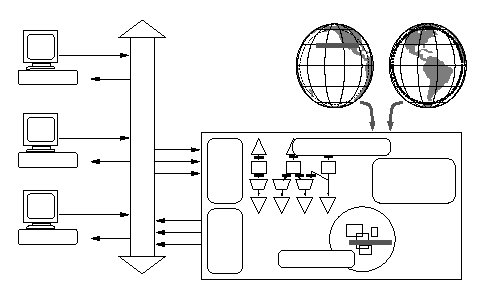
\includegraphics{figs/overview.fig.eps}%
\end{picture}%
\setlength{\unitlength}{4144sp}%
%
\begingroup\makeatletter\ifx\SetFigFontNFSS\undefined%
\gdef\SetFigFontNFSS#1#2#3#4#5{%
  \reset@font\fontsize{#1}{#2pt}%
  \fontfamily{#3}\fontseries{#4}\fontshape{#5}%
  \selectfont}%
\fi\endgroup%
\begin{picture}(3431,2004)(79,-1198)
\put(136,322){\makebox(0,0)[lb]{\smash{{\SetFigFontNFSS{5}{6.0}{\familydefault}{\mddefault}{\updefault}{\color[rgb]{0,0,0}connect}%
}}}}
\put(2858,-421){\makebox(0,0)[lb]{\smash{{\SetFigFontNFSS{6}{7.2}{\familydefault}{\mddefault}{\updefault}{\color[rgb]{0,0,0}Stream}%
}}}}
\put(2858,-556){\makebox(0,0)[lb]{\smash{{\SetFigFontNFSS{6}{7.2}{\familydefault}{\mddefault}{\updefault}{\color[rgb]{0,0,0}Generator}%
}}}}
\put(136,-308){\makebox(0,0)[lb]{\smash{{\SetFigFontNFSS{5}{6.0}{\familydefault}{\mddefault}{\updefault}{\color[rgb]{0,0,0}connect}%
}}}}
\put(136,-893){\makebox(0,0)[lb]{\smash{{\SetFigFontNFSS{5}{6.0}{\familydefault}{\mddefault}{\updefault}{\color[rgb]{0,0,0}connect}%
}}}}
\put(1621,-196){\rotatebox{270.0}{\makebox(0,0)[lb]{\smash{{\SetFigFontNFSS{6}{7.2}{\familydefault}{\mddefault}{\updefault}{\color[rgb]{0,0,0}Parser}%
}}}}}
\put(2206,-196){\makebox(0,0)[lb]{\smash{{\SetFigFontNFSS{6}{7.2}{\familydefault}{\mddefault}{\updefault}{\color[rgb]{0,0,0}Optimization}%
}}}}
\put(1621,-691){\rotatebox{270.0}{\makebox(0,0)[lb]{\smash{{\SetFigFontNFSS{6}{7.2}{\familydefault}{\mddefault}{\updefault}{\color[rgb]{0,0,0}Delivery}%
}}}}}
\put(1486, 29){\makebox(0,0)[lb]{\smash{{\SetFigFontNFSS{6}{7.2}{\familydefault}{\mddefault}{\updefault}{\color[rgb]{0,0,0}\acs{DSMS} Server}%
}}}}
\put(2138,-1066){\makebox(0,0)[lb]{\smash{{\SetFigFontNFSS{6}{7.2}{\familydefault}{\mddefault}{\updefault}{\color[rgb]{0,0,0}Execution}%
}}}}
\put(1396,704){\makebox(0,0)[lb]{\smash{{\SetFigFontNFSS{6}{7.2}{\familydefault}{\mddefault}{\updefault}{\color[rgb]{0,0,0}Weather Satellites}%
}}}}
\end{picture}%
}
  \caption{\ac{GS} database system}
  \label{fig:overview}
\end{figure}

Multiple users connect to a server and formulate queries to the
system.  The system is optimized for continuous queries on the input
satellite stream of data.  The queries are parsed and validated, then
optimized.  Optimization includes single and multi-query methods,
combining queries to minimize computation time and/or the number and
size of intermediate images that are created and maintained in the
system.  Minimizing the size of images typically reduces both memory
usage and computational burden.  New queries affect the execution plan
for the system, but these changes are made at specific times because
the execution is continuously working on the incoming \ac{RSI} stream.
This stream comes from a separate module that re-interprets the raw
data into a format more suitable for query processing.

Query execution is highly dependent on the structure of the incoming
data.  The \ac{RSI} data is manipulated one row at a time.  This
matches the form of the satellite stream and is also convenient for
multi-query optimizations.  Figure~\ref{fig:rsi-example} shows a
notional example of how data is scanned and transmitted by a
geostationary satellite.

\begin{figure}[htb]
  \centering
  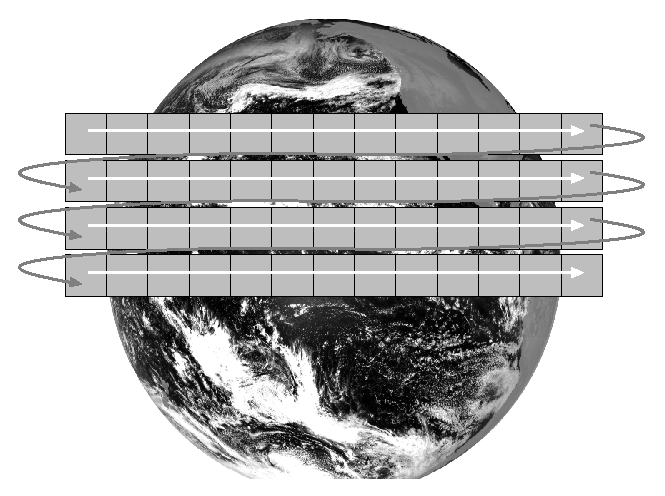
\includegraphics[width=5cm]{figs/rsi-example.fig.eps}  
  \caption{\ac{RSI} data stream}
  \label{fig:rsi-example}
\end{figure}

The query execution includes final operators designed to return the
data back to the clients, which requires persistent or synchronous
connections on both the server and the client sides.

Images and image manipulation will be described with an image algebra,
a rigorous and compact method for describing images, image
transformations, and image analysis~\cite{ritter01handb-comput}.
Image algebra is a many-valued algebra that includes \emph{Point
  Sets}, \emph{Value Sets} and \emph{Images}.  \emph{Points Sets} are
the points in space and time with defined values.  \emph{Value Sets}
are the values associated with the points in the point set.
\emph{Images} can be thought of as functions mapping points to values,
or as a set of point value pairs.  These individual pairs are the
\emph{pixels} in the image.

Image operations are the basic building blocks for queries to the
system.  These operations include functional operations, image
restrictions to specific point sets of interest, spatial transforms on
images from one point set to another, and neighborhood operations
where multiple pixels from an image are combined to a single value.

Defined operations on or among images include any operation that
operates on the value set \vs{V}, which extends to a natural
\emph{Induced operation} on \vs{V}-valued images.  \emph{Image
  restrictions} return image subsets restricted to a given point set.
Restrictions are possibly the most important of all operations, and
flexible methods for defining new point sets need to be included in
the query formulations.  This is especially true in this model where
point set restrictions define not only spatial, but also
spatio-temporal limits on incoming data streams.  

\emph{Spatial transformations} map an image from one point set to
another.  Spatial transformations are used for magnification, rotation
and general affine transformations.  The most common spatial
transformation converts the satellite point set to the point set grid
requested by the queries.  Each query can specify pixel locations and
resolutions that differ from the input images.

One component of these transformations is to project satellite data
to new coordinate systems.  Data as it is received from the \ac{GOES}
satellite is in its own perspective projection.  Many applications
and users would prefer data to be delivered in a more standard Earth
coordinate system.  For example, Figure~\ref{fig:ll} shows a
comparison of the \ac{GOES} visible channel, in both its native
projection, and projected to longitude-latitude (equidistant
cylindrical).

\begin{figure}[htb]
  \centering
  \subfigure[GOES-10]{
    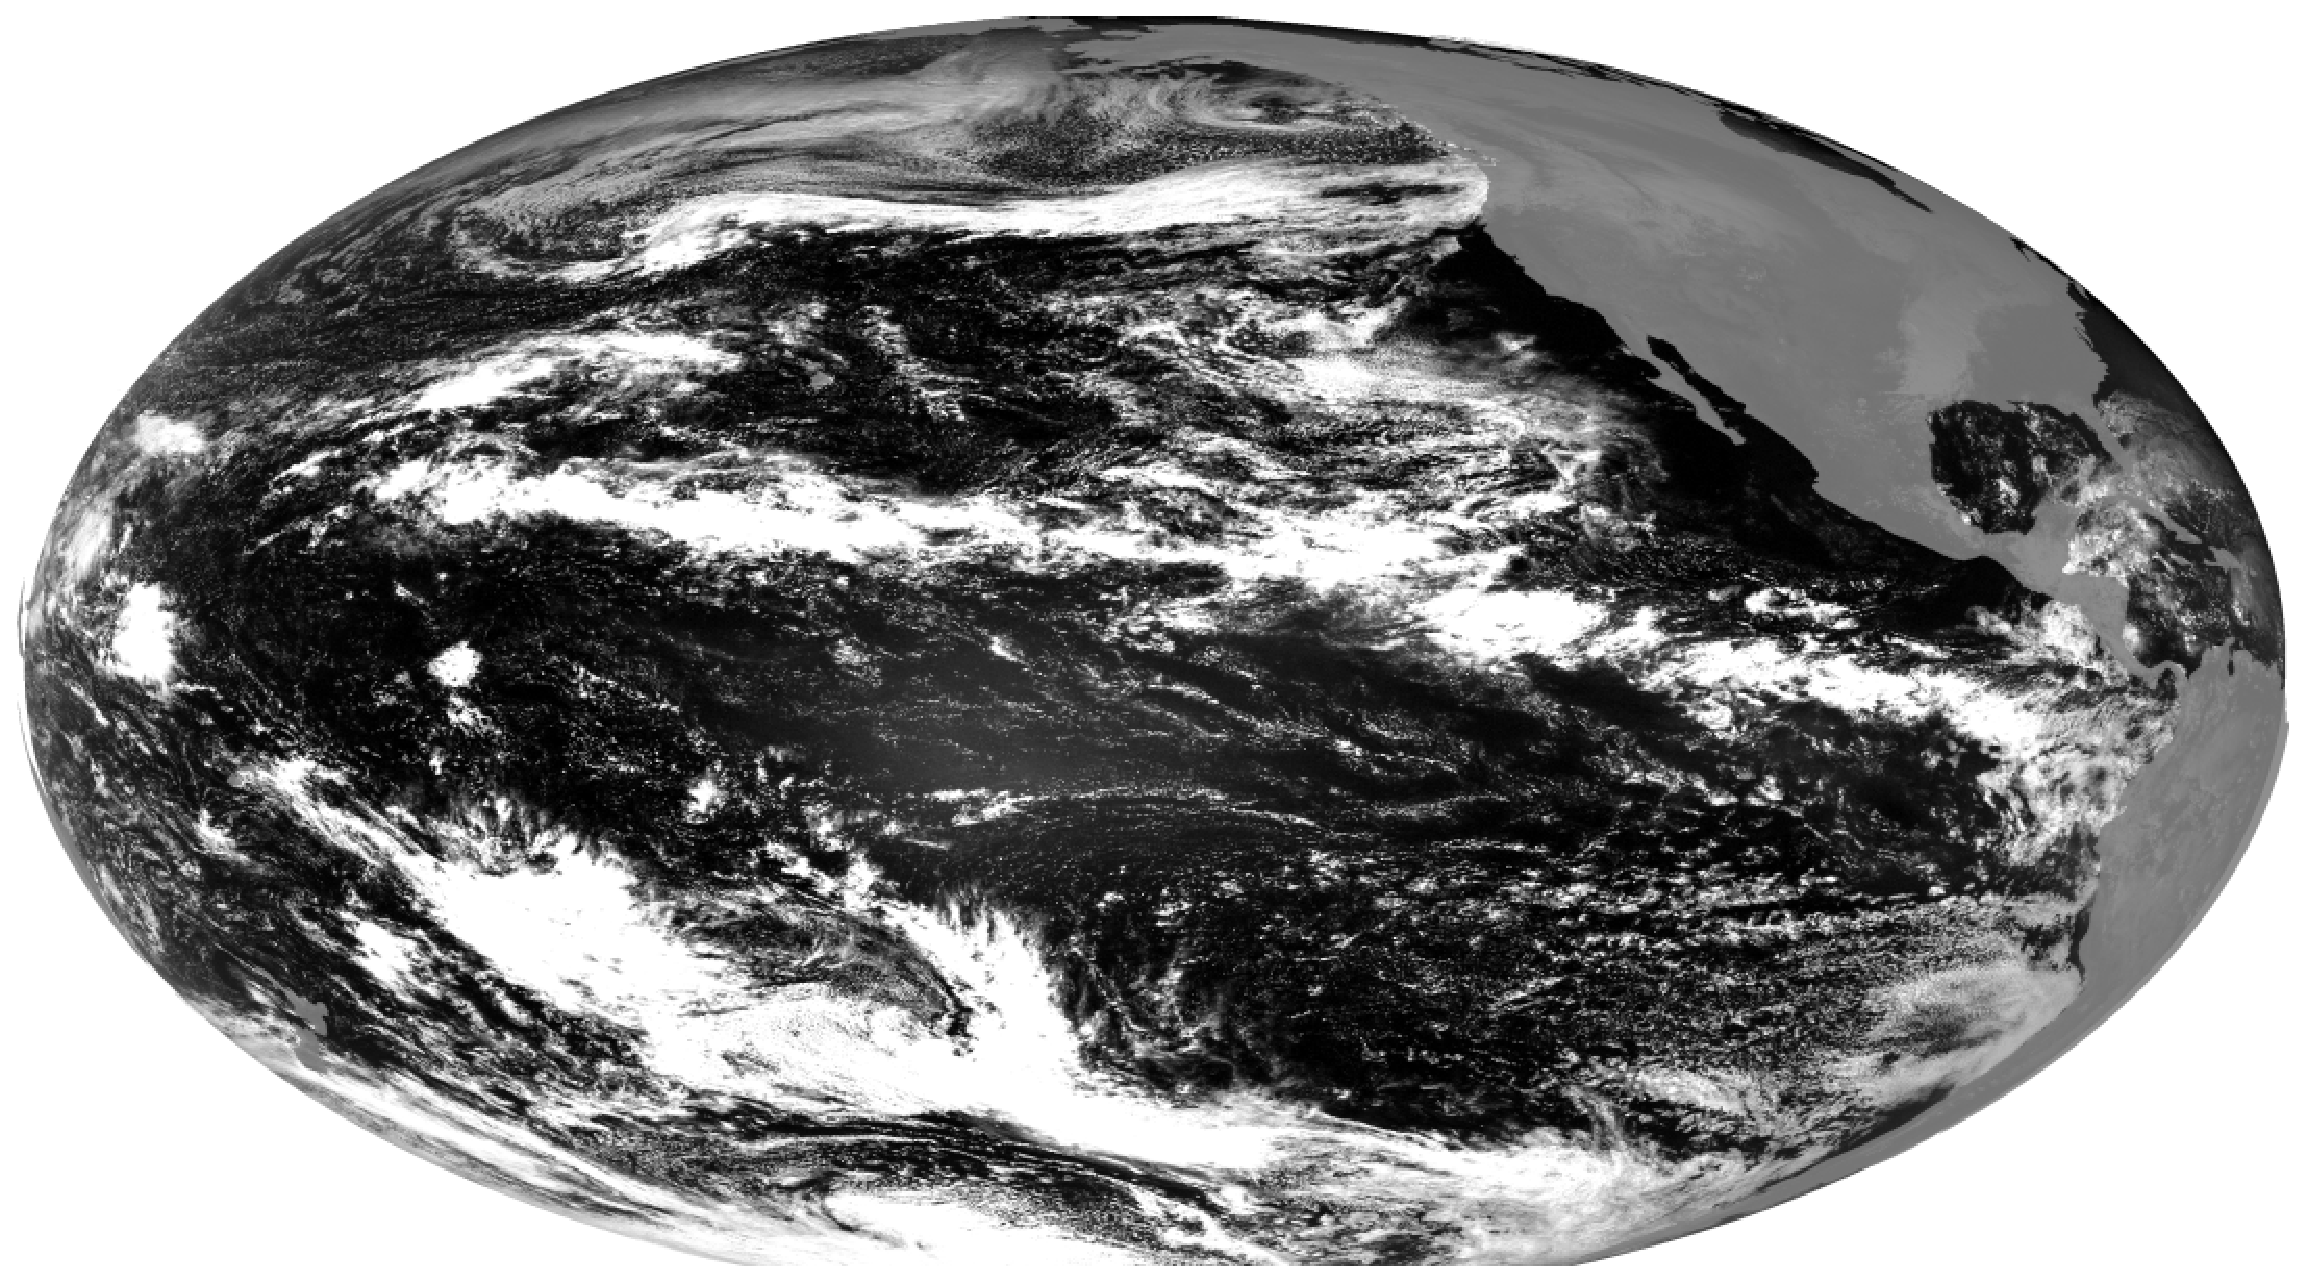
\includegraphics[height=5.0cm]{figs/projection/goes}
  }
  \subfigure[Latitude Longitude]{
    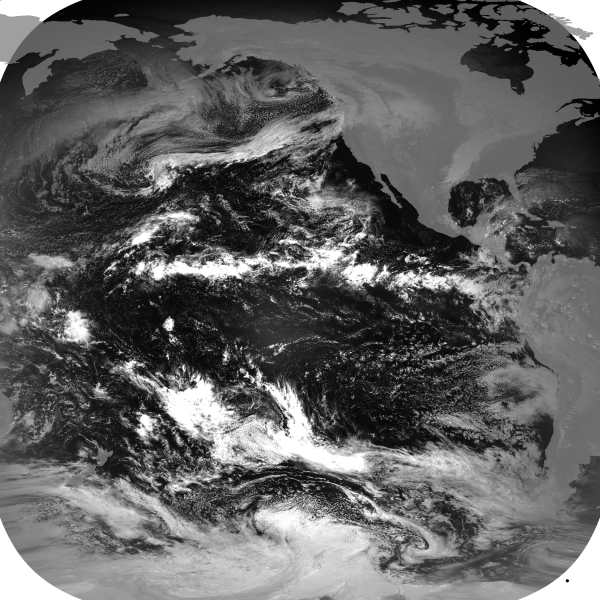
\includegraphics[height=5.0cm]{figs/projection/ll}
  }
\caption{The \ac{GOES} satellite projection. }
\label{fig:ll}
\end{figure}


\emph{Neighborhood operations} allow for multiple pixels from a single
image to be combined to create a single pixel value in a new image.
Neighborhoods allow for aggregation functions like averaging, edge
detection, speckle removal, and other operations.

Queries in the \ac{GS} project do not build on a variant of the SQL
syntax, but on something closer to the image algebra representation
and on specialized interfaces.  The specific query declaration uses a
formulation inspired by \ac{WMS} specification~\cite{openg04web-map}.
Users specify a specific data product, coordinate system, spatial
extents and pixel size via the resultant image height and width.
Temporal restrictions can also be identified.

Queries can be made on other data products besides the satellite image
channels.  Data products like image channel ratios can be specified as
long as the index itself is identified as a specific product by the
server.  The specification further simplifies query formulation by
standardizing and simplifying both spatial transforms and restrictions
to a limited but well-defined subset.  More formally, these queries
can be identified as a particular expression in an image algebra
formulation, including a restriction, induced operation, neighborhood
operation, and coordinate system transformation, where all operations
are compactly described in a standard way.  This simple interface does
not allow for a sophisticated set of user queries, but it does satisfy
the most basic requirements of serving many spatial restrictions and
geometric transformations to many clients.

Query optimization attempts to limit the processing time and/or the
amount of memory usage for the \ac{DSMS} as a whole.  Query
optimization is primarily concerned with two goals: query rewriting to
limit the amount of work done in the system, and finding common
subsets within the queries active against the image stream, which
allow results to be shared among multiple queries.

First, individual queries are rewritten to optimize their individual
execution, the queries are then optimized in a multi-query fashion.
Multi-query optimization centers around grouping similar query
components into a single operation that works simultaneously for a
group of queries.  In \ac{DSMS} research this has multiple conceptual
definitions, including grouped filters~\cite{madden02contin-adapt} and
query indexing~\cite{prabhakar02qindex}.  Figure~\ref{fig:query-eval}
shows a typical query index scheme for a spatial restriction
operation, where rather than each query requiring its own restriction
operator, a single restriction module has indexed the point sets of a
number of active queries.  For each continuous user query, a region,
$R_i$, is associated that describes the \acf{ROI} for that query.  For
incoming \ac{RSI} data, it is determined what data is relevant to what
user queries and which queries can share incoming data.

\begin{figure}[htb]
  \centering
  \scalebox{2}{\begin{picture}(0,0)%
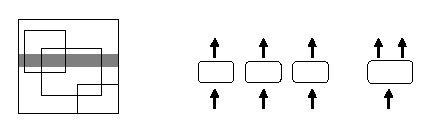
\includegraphics{figs/query-eval.fig.eps}%
\end{picture}%
\setlength{\unitlength}{4144sp}%
%
\begingroup\makeatletter\ifx\SetFigFont\undefined%
\gdef\SetFigFont#1#2#3#4#5{%
  \reset@font\fontsize{#1}{#2pt}%
  \fontfamily{#3}\fontseries{#4}\fontshape{#5}%
  \selectfont}%
\fi\endgroup%
\begin{picture}(3030,792)(-11,59)
\put(2686,419){\makebox(0,0)[lb]{\smash{{\SetFigFont{5}{6.0}{\familydefault}{\mddefault}{\updefault}{\color[rgb]{0,0,0}\dct}%
}}}}
\put( 91,659){\makebox(0,0)[lb]{\smash{{\SetFigFont{5}{6.0}{\familydefault}{\mddefault}{\updefault}{\color[rgb]{0,0,0}$R_1$}%
}}}}
\put(226,299){\makebox(0,0)[lb]{\smash{{\SetFigFont{5}{6.0}{\familydefault}{\mddefault}{\updefault}{\color[rgb]{0,0,0}$R_2$}%
}}}}
\put(496,164){\makebox(0,0)[lb]{\smash{{\SetFigFont{5}{6.0}{\familydefault}{\mddefault}{\updefault}{\color[rgb]{0,0,0}$R_3$}%
}}}}
\put(811,479){\makebox(0,0)[lb]{\smash{{\SetFigFont{5}{6.0}{\familydefault}{\mddefault}{\updefault}{\color[rgb]{0,0,0}RSI}%
}}}}
\put(1416,738){\makebox(0,0)[lb]{\smash{{\SetFigFont{5}{6.0}{\familydefault}{\mddefault}{\updefault}{\color[rgb]{0,0,0}$Q_1$}%
}}}}
\put(1787,738){\makebox(0,0)[lb]{\smash{{\SetFigFont{5}{6.0}{\familydefault}{\mddefault}{\updefault}{\color[rgb]{0,0,0}$Q_2$}%
}}}}
\put(2157,738){\makebox(0,0)[lb]{\smash{{\SetFigFont{5}{6.0}{\familydefault}{\mddefault}{\updefault}{\color[rgb]{0,0,0}$Q_3$}%
}}}}
\put(1388,404){\makebox(0,0)[lb]{\smash{{\SetFigFont{5}{6.0}{\familydefault}{\mddefault}{\updefault}{\color[rgb]{0,0,0}$R_1$}%
}}}}
\put(1748,404){\makebox(0,0)[lb]{\smash{{\SetFigFont{5}{6.0}{\familydefault}{\mddefault}{\updefault}{\color[rgb]{0,0,0}$R_2$}%
}}}}
\put(2108,404){\makebox(0,0)[lb]{\smash{{\SetFigFont{5}{6.0}{\familydefault}{\mddefault}{\updefault}{\color[rgb]{0,0,0}$R_3$}%
}}}}
\put(1441, 74){\makebox(0,0)[lb]{\smash{{\SetFigFont{5}{6.0}{\familydefault}{\mddefault}{\updefault}{\color[rgb]{0,0,0}RSI}%
}}}}
\put(1801, 74){\makebox(0,0)[lb]{\smash{{\SetFigFont{5}{6.0}{\familydefault}{\mddefault}{\updefault}{\color[rgb]{0,0,0}RSI}%
}}}}
\put(2161, 74){\makebox(0,0)[lb]{\smash{{\SetFigFont{5}{6.0}{\familydefault}{\mddefault}{\updefault}{\color[rgb]{0,0,0}RSI}%
}}}}
\put(2746, 74){\makebox(0,0)[lb]{\smash{{\SetFigFont{5}{6.0}{\familydefault}{\mddefault}{\updefault}{\color[rgb]{0,0,0}RSI}%
}}}}
\put(2656,749){\makebox(0,0)[lb]{\smash{{\SetFigFont{5}{6.0}{\familydefault}{\mddefault}{\updefault}{\color[rgb]{0,0,0}$Q_1'$}%
}}}}
\put(2836,749){\makebox(0,0)[lb]{\smash{{\SetFigFont{5}{6.0}{\familydefault}{\mddefault}{\updefault}{\color[rgb]{0,0,0}$Q_2'$}%
}}}}
\end{picture}%
}
  \caption{Multi-query restriction operation} 
\label{fig:query-eval}
\end{figure}

By developing modules for the basic image operations that can take as
input a single \ac{RSI} stream and distribute results to multiple
output streams, a \acf{QEP} is developed as a number of these
operators joined together for a complete system.  This allows not only
the pipelining of image data to operators to which the data is of
interest, but it also facilitates the sharing of image data among
queries that have overlapping \acp{ROI}.

Query execution is tied intrinsically to the query plan developed by
the optimizer, and also by the organization of the incoming data
stream.  In developing the \ac{GS} architecture, modules are developed
for each of the basic image operations, which apply to more than one
query in a single operation.  The modules are linked together for
complete query execution.  As mentioned, the \ac{RSI} data stream
comes in an ordered row-by-row arrangement.  This organization plays
an important role in developing image operators and determining how
modules in the query plan are arranged.  By developing stream-oriented
operators that work on these image rows, a system can be developed
that uses minimum amounts of memory, and can deliver data in near
real time.

Figure~\ref{fig:query-eval} shows an example module for processing
multi-query image restrictions.  For the restriction module, the
\acf{DCT}~\cite{hart04index-query,DBLP:conf/ssd/HartGZ05} is proposed
as a space efficient structure to index \acp{ROI} that are part of
more complex queries against \ac{RSI} data streams. The spatial trends
inherent to most types of streaming \acs{RSI} data are exploited to
build a small index that is especially efficient when the incoming
stream data is in close spatial proximity.  Queries can be answered
very quickly if the next data stream segment has the same result as
the previous query and will incrementally update a new result set when
the result is different.  Based on the information provided by the
\ac{DCT}, incoming data can be pipelined to respective query
operators, providing the basis for multiple-query processing models
for streaming RSI data.

\section{Objectives}

The overall goals of the \ac{GS} project were to investigate
processing strategies for query processing of \ac{RSI} streams, to
provide tools for efficient processing, and to develop a complete
system for interfacing with a satellite image stream.  The system
answers continuous queries from multiple users.  Specific objectives
for the research included:

\begin{itemize}

\item Identify a data and query model that is natural for users,
  researchers and application developers, as well as concise and
  unambiguous.  The models need to be simple enough to be easily
  understood, but with enough richness to satisfy a large class of
  data and query specifications.  Develop a simple query syntax to
  represent the query model.

\item Define a core set of operators that provide sufficient support
  for answering user queries on \ac{RSI} data.  These operators should
  naturally follow from the data and query model, and
  represent an implementation of those models.

\item Develop query optimizations that allow a \ac{DSMS} system to
  tailor its \acf{QEP} to the currently active queries.  Optimizations
  include query rewriting to optimize each individual query.
  Multi-query optimization techniques designed to a share operators
  and common data among queries will also be examined.

\item Create specialized operators that take advantage of the highly
  organized structure that is common in \acf{RSI} data.

\item Design studies to validate query optimization techniques.  These
  studies will test the operational parameters of individual
  components of the \ac{QEP}.  In addition, overall \acp{QEP} will be
  compared to similar systems running without such multi-query
  optimization strategies.

\item Architect the design of a complete on-line system for processing
  continuous queries from multiple users.  A processing design could
  be developed for use with an existing \ac{GIS} and image processing
  application.  In addition, a ground up implementation designed
  specifically with the streaming nature of the incoming \ac{RSI} data
  will be described.

\end{itemize}


\section{Summary of Results}

The research carried out to address the above objectives focuses on
applications dealing with real-time weather satellite imagery.  In
particular, \acf{NOAA} \acf{GOES} satellite~\cite{goes96databook} was
used as the input \ac{RSI} data stream to the system, and all queries
were made to this stream.  The \ac{GOES} program is one of the most
important meteorological programs in the United States and offers an
imaging instrument with five radiometric channels for a variety of
applications, including cloud identification and tracking, atmospheric
water measurement, absorbed solar energy, and thermal studies of
clouds and Earth surfaces.

The \ac{DSMS} applications developed allow multiple users to connect
to a server to receive this \ac{RSI}.  A simple, but effective
interface allows users access to most needed set of queries to the
system.

Major results from this research correspond to the chapters of this
work and are summarized below.

\subsection*{The \ac{GS} Model, Chapter~\ref{cha:models}}

A data and query model was developed based on image algebra, described
in detail in Chapter~\ref{cha:models}.  Additional specifications
particular to the \ac{GS} architecture are added to an image algebra
to provide concrete semantics for streaming \ac{RSI} imagery.  Some
image algebra operators were altered to allow for point sets of
indeterminate length.

Queries are defined as image algebra expressions.  A small subset of
expressions are allowed as queries.  In particular, a simple syntax
using the \acf{WMS} interface was adopted for queries.

The basic query processing operators were developed from the model
based in the image algebra and the allowed query expressions.  In
particular, operators for \emph{induced operation},
\emph{restrictions}, \emph{spatial transformations}, and
\emph{neighborhood operations} were defined.  Rules for expression
rewriting were also introduced.


\subsection*{Query Processing, Chapter~\ref{cha:query}}

One major feature of an effective query processor is choosing an
optimal execution plan for a given query.  Because queries are in
image algebra, specialized rules regarding the rewriting of image
algebra expressions are developed.  A strategy is introduced to create
an optimal or ``best-effort'' \ac{QEP}.  Both single query optimizations
and multi-query optimizations are utilized.

Single query optimization deals with rewriting a query to be more
efficient in its computation.  For a single query, optimizations
concern the ordering of the operators.  Multi-query optimization adds
additional savings by sharing results between queries to develop
a single global \ac{QEP}.

\subsection*{Multi-Query Optimization with Existing GIS
  Applications, Chapter~\ref{cha:existing}}

The processing improvements from single and multi-query optimization
techniques is dependent on both the implementation of the individual
operators and on the make-up of the current queries within the system.
The savings of a multi-query \ac{QEP} are quantified using an existing
application framework, a real \ac{RSI} image stream, and real world
query parameters.

The application framework chosen is the \acf{GRASS}.  \ac{GRASS} has
no notion of image streams and, like most \ac{GIS} applications, works
on discrete images in secondary storage.

Experimental results using predicted query patterns over the visible
hemisphere of the weather satellite indicate that developing
multi-query optimized plans can improve performance significantly when
compared to queries executed separately.


\subsection*{The Dynamic Cascade Tree, Chapter~\ref{cha:dct}}

Multi-query optimization techniques require an operator that is able
to provide restrictions for multiple query \acp{ROI}.  \ac{RSI} rows
enter the system with high frequency and there can be many individual
\acp{ROI}, and many restriction operators handled in a \ac{QEP}.
Also, the on-line implementation of the spatial transformation
operator requires a restriction operation with many \acp{ROI}, one per
output row.

To satisfy these needs, an index named the \acf{DCT} was developed,
which indexes spatio-temporal \acp{ROI}.  The \ac{DCT} is designed to
exploit the spatial trends in incoming \ac{RSI} data to provide a very
efficient index.  Experimental results using both random input and
\acf{GOES} data give a good insight into restrictions on streaming \ac{RSI}
and verify the efficiency and utility of the \ac{DCT}.

\subsection*{Multi-Query Execution using an Online System,
  Chapter~\ref{cha:operators}}

An on-line \ac{DSMS} for \ac{RSI} data is designed in
Chapter~\ref{cha:operators}.  A \ac{DSMS} system designed specifically
for \ac{RSI} data operates on smaller discrete parts of an image
directly as they arrive.  Input image data is manipulated a single row
at a time.  This is most consistent with the data stream arrival
pattern and allows for the smallest in-memory footprint of the
processing system.  The \ac{DSMS} is divided into three main
components, the \acf{QM}, \emph{Row Memory}, and \emph{Query Data
 Management}.

The \ac{QM} is the main component.  It creates a \acf{QEP} for the
system, creates needed operators, and executes the plan.  The \ac{QM}
also includes implementations of the individual operators; an
implementation for general induced operations; a restriction operator
designed to allow multiple restrictions to be satisfied
simultaneously; a halving operator for averaging; and a spatial
transformation operator for image projection.

The \emph{Row Memory} component provides an interface to create,
subset, and destroy rows of data in the system.  The \emph{\ac{GVAR}
  Input} handles the interface to the \ac{GVAR} data stream and
creates rows for input into the system.  \emph{Query Data Management}
provides support for making the data available to the users, including
formatting images and distributing results.


\section{Reference Queries}
\label{sec:queries}

Tables~\ref{tab:ref-queries} and~\ref{tab:ref-queries-desc} describe
an example set of queries that might be run against an \ac{RSI}
\ac{DSMS} system.  These queries will be revisited throughout the
paper and will be used to illustrate important aspects of query
optimization and execution.  Because of their role, the queries are
chosen for their suitability as examples and not as a representative
cross section.  For example, the input streams are limited to a small
number of channels from a single satellite, to increase in interplay
between the queries.
%
\begin{table}[htb]
  \centering
  \caption{Example queries}
  \begin{tabular}[b]{c|c|c|c|c|c}
    {\bf Q } & {\bf Product} & {\bf \acs{ROI}} & {\bf Time} & {\bf Projection} & {\bf Resolution} \\
    \hline \hline
    \qry{A} & $C1$ & Mexico & Always & GOES &$\approx$\unit[1]{km$^2$} \\
    \qry{B} & $C1$ & N. America & Always & Lat/Long & $\approx$\unit[4]{km$^2$} \\
    \qry{C} & NDVI$(C1,C2)$ & N. America & Always & GOES & $\approx$\unit[4]{km$^2$} \\
    \qry{D} & NDVI$(C1,C2)$ & Hemisphere & Always & Lat/Long & $\approx$\unit[8]{km$^2$} \\
    \qry{E} & $C1$ & N. America & Time$=\pt{t}$ & GOES & $\approx$\unit[1]{km$^2$} \\ 
    \qry{F} & $C1$ & California & Days $<\pt{d}$   & UTM  & \unit[1]{km$^2$} \\
    \qry{G} & $C1$ & Point \pt{G} & Always & N/A & N/A \\
    \qry{H} & $C1$ & Pixel Values $> v$ & Always   & GOES & \unit[1]{km$^2$} \\
  \end{tabular}
  \label{tab:ref-queries}
\end{table}
%
\begin{table}[htb]
  \caption{\ac{GOES} queries}
  \centering
  \begin{tabular}{>{}c|>{\PBS\raggedright\hspace{0pt}}p{13cm}}

    {\bf Q} & \multicolumn{1}{c}{\bf Description} \\

    \hline
    \hline

    \qry{A} & Query A represents a user requesting Channel 1, (visible) data over a \ac{ROI} covering Mexico.  There are no time constraints on the query.  The resolution corresponds to the default \ac{GOES} data, as does the requested projection \\

    \hline

    \qry{B} & Query B is another query on the visible channel, however in this instance, the user wants the data at a coarser resolution, and projected to a longitude-latitude, (equidistant cylindrical) grid. \\

    \hline

    \qry{C} & This query represents a user requesting a product, in 
    this case NDVI, which is a normalized difference index using two input channels.  This query is limited to North America. \\

    \hline

    \qry{D} & This query represents an NDVI request at a coarse scale and covering the entire northern hemisphere. The requested image is also projected to longitude-latitude. \\

    \hline    

    \qry{E} & This query requests visible GOES data, but
      only the image that occurs at some time, \pt{t}, everyday. \\

    \hline

    \qry{F} &  This is similar to the query \qry{E}, but also specifies an ending date, \pt{d}, when the query will end. \\

    \hline

    \qry{G} & This query asks for image data at a single point.\\

    \hline

    \qry{H} &  Channel 1, but only in the image where the \emph{pixel values} are greater than some amount $v$. \\ 

  \end{tabular}
  \label{tab:ref-queries-desc}
\end{table}

\chapter{Background}
\label{cha:background}


The \ac{GS} architecture draws from work in \acf{GIS}, including remote
sensing, image processing, meteorological satellites, and geospatial
databases.  In addition, ideas are drawn from \acf{DSMS} research.  In
this chapter, these areas are reviewed from both a technical and
historical perspective.

\section{Geographic Information Systems}

A \acf{GIS} is a system designed to create, store, edit and maintain
geographic information.  More generally a \ac{GIS} is a combination of
computer software along with geographic data that allows users to
interactively query spatial data, analyze that information, and
support decision making.  The term \acl{GIS} is something of an open
ended term as it deals with any data having a geographic component.
It covers a large number of disciplines.  The focus here is on the
development of \ac{GIS} tools that have been developed in support of
processing, storing, managing and distributing remote sensing data.

Remote sensing, in contrast to in-situ measurements, is the
process of acquiring information about something without being in
physical contact with the object.  Typically, remote sensing
applications involve obtaining information about the Earth from
sensors at some distance from the surface.  Remote sensing instruments
detect reflected or emitted energy from the surface and make
inferences about the properties of the surface based on that
information.  The field of remote sensing is large and includes
studies describing image processing
methods~\cite{mather04comput-proces}, applications oriented towards
environmental studies~\cite{curtis99introd-envir, hinton96gis-remot,
  skidm02envir-model}, and more general
descriptions~\cite{atkin99advan-remot}.

\subsection{Remote Sensing}

In a very real way, remote sensing has its roots in pre-history, as
people are in possession of one the finest remote sensing devices
devised, the eye.  Largely because of the anthropogenic basis of
remote sensing, it is a technology that has been embraced in a wide
array of disciplines.

Remote sensing as a science closely follows the advent of photography.
The first natural photographic image was taken in 1827.  By the 1850's
multiple techniques existed for sharp images with relatively short
exposure times.  In 1855, a patent on using aerial photography for
mapping was issued, and the first aerial images were taken from a
balloon in 1858.  Aerial photographs may have been used for military
purposes as early as the Civil War in the 1860's.  By the late 1880's
and into the early 1900's, aerial photography was being used for
environmental studies, military campaigns, and even the first rocket
launched imagery.  World War I provided a boost in the science of
photo interpretation, and by the 1920's, books were being written
about the subject~\cite{reeves27aerial-photog,
  winchester28aerial-photog}.  World War II encouraged more
sophistication in interpretation, as well as more products, including
the first infrared film, which allowed for more sophisticated
interpretations, especially vegetation studies.  The 1960's marked the
beginning of imaging satellite systems, beginning with the first
meteorological satellite, the \ac{TIROS} (Figure~\ref{fig:tiros}),
launched in 1960.  These satellites were equipped with a television
camera that radioed images back to Earth, offering meteorologists an
important new tool.  1960 also saw the launch of the first US spy
satellite, a top secret program code named CORONA.  At its peak in the
late 60's and early 70's, CORONA satellites were acquiring images with
2 meter resolution (Figure~\ref{fig:corona}).  The photographs were
parachuted back from space.  The CORONA program was only declassified
in 1995, and the images are now available for purchase from the
\ac{USGS}.

\begin{figure}[htb]
  \centering
  \subfigure[TIROS-1 (with markup)]{
    \label{fig:tiros}
    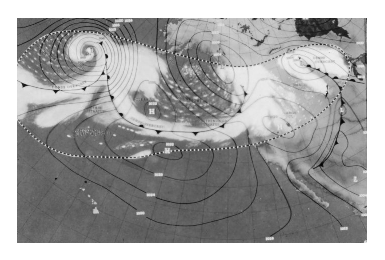
\includegraphics[width=0.45\textwidth]{figs/tiros-1.eps}
    } \quad
    \subfigure[CORONA]{
      \label{fig:corona}
    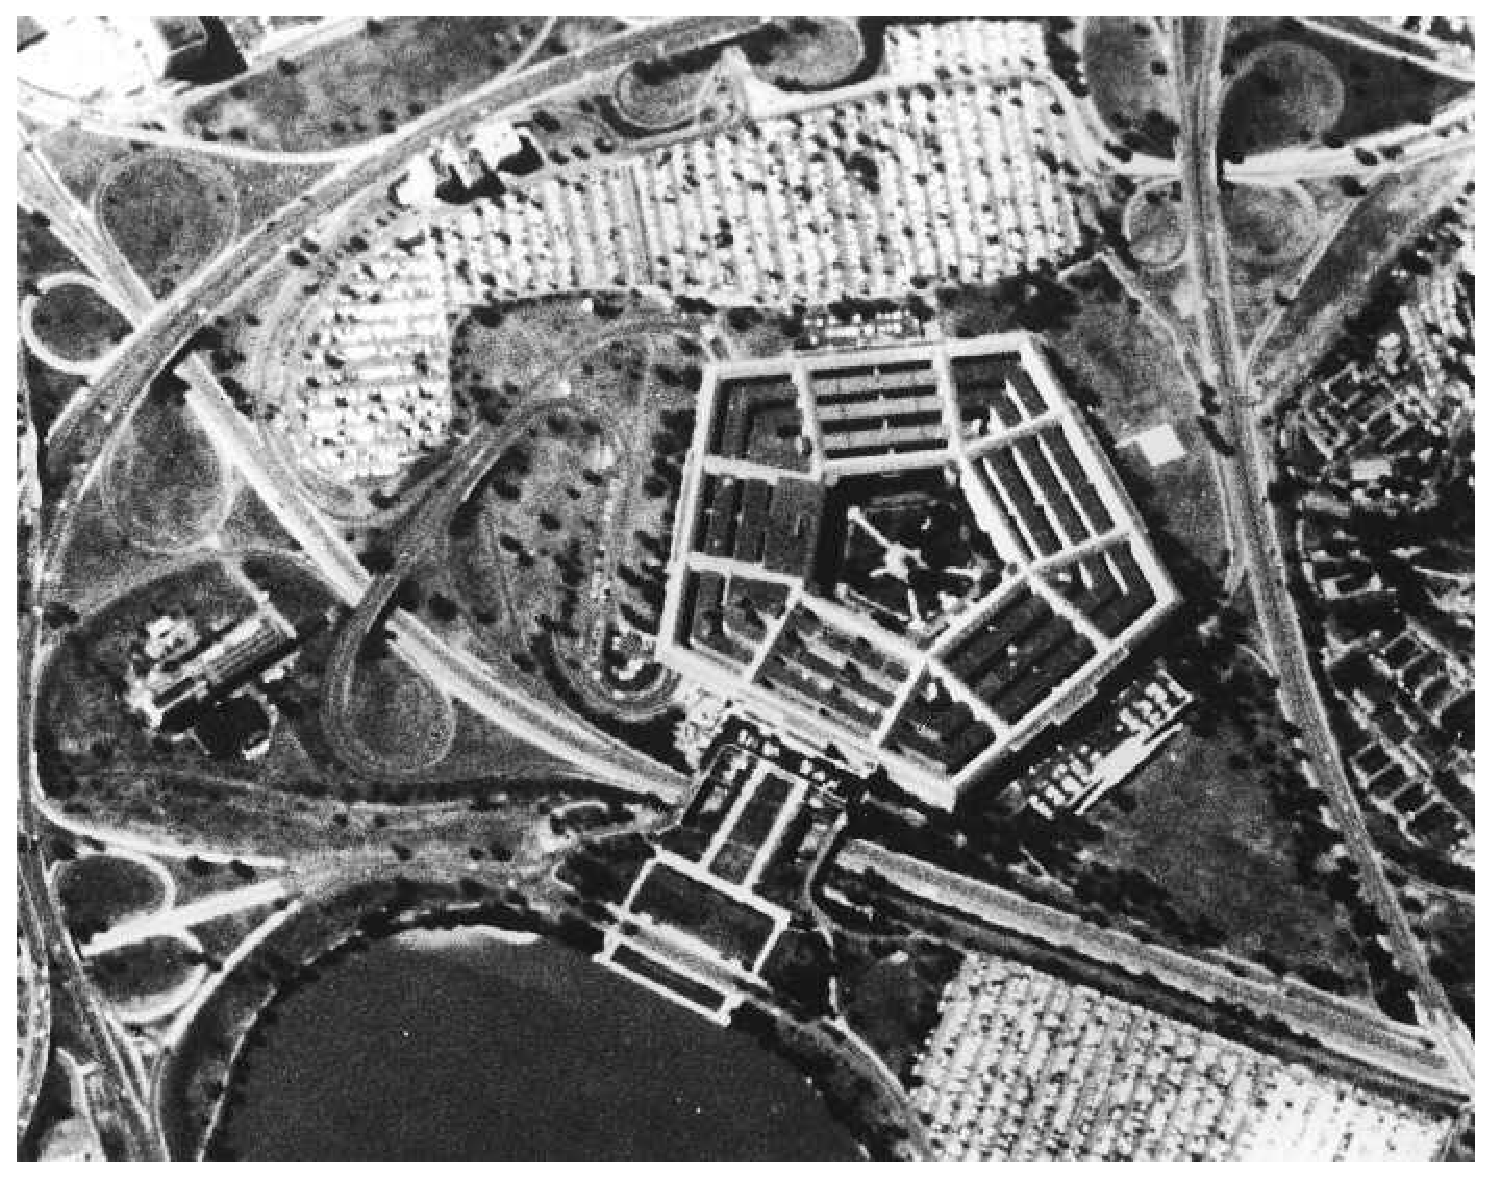
\includegraphics[width=0.45\textwidth]{figs/corona.eps}
    }
  \caption{Early satellite images}
  \label{fig:early-satellites}
\end{figure}

\ac{TIROS} heralded a new discipline of digital image processing of
\acf{RSI}.  More general \ac{GIS} applications were also being
developed~\cite{dangermond92what-is, landgrebe86brief-histor}.  At
this time, main-frame computers and specialized hardware were required
for any image processing.

The Nimbus meteorological program, and the \ac{ERTS}, later renamed
Landsat, environmental satellite program both began in the early
1970's, and further advanced remote sensing.  The \ac{LACIE} program,
started in 1974, was one of the first programs researching the
application of digital remote sensing to environmental studies, in
this case for determining global wheat crop
yields~\cite{chhikara78lands-based,swain85advan-inter}.

The 1980's and 1990's saw a dramatic increase in the number of
satellites launched, in the image processing algorithms developed, and
in the number of users of \ac{GIS} and image processing software.  In
1988 the \acf{NCGIA} was founded in response to a \acf{NSF} call for
proposals.  The \ac{NCGIA}'s general mission is to advance research in
\ac{GIS} science, with focus on modeling, spatial accuracy, cognition,
and other research areas.  For image processing, the U.S. Army Corp of
Engineering Research Laboratories (USA-CERL), developed the
\acf{GRASS} from 1982 until 1995~\cite{GRASS_GIS_software,wiki06}.
One of the first fully featured raster based \acp{GIS}, \ac{GRASS} was
developed for management and planning applications, and has grown a
wide range of tools for a variety of applications.  \ac{GRASS} is
currently developed in the public domain, and continues with active
development, including new versions with enhanced capabilities, and
new graphical front end applications, such as
\ac{QGIS}~\cite{wiki06}.

In terms of general purpose \ac{GIS} systems, a leader in the field is
\acf{ESRI}~\cite{wiki06}.  \ac{ESRI} was founded in 1969, but started
developing a core \ac{GIS} computing application, ARC/INFO in 1982.
Originally dealing with only point, line and polygon data, the suite
of \ac{ESRI} tools began incorporating image processing in the late
1980's and early 1990's.  The current image processing and remote
sensing applications include a wide array of processing algorithms,
tight interaction with vector \ac{GIS} data, and object oriented image
classification~\cite{wiki06}.

The \acf{EOS}, a \acs{NASA} program having launched over twenty
instruments designed for global monitoring of the Earth's land, sea,
and atmospheric processes, is the current state of the art in remotely
sensed image acquisition and also data collection and distribution.
The first \ac{EOS} satellite was launched in 2000.

Today, there are over 800 satellites in space, more then 150 of which
have some remote sensing instrumentation.  More than half of these are
operated by the United States~\cite{concerned06ucs-satel-datab}.  More
and more users are using \ac{GIS} and image processing in a growing
set of diverse applications.


\subsection{\acf{GOES}}
\label{sec:rsi}

Kidder~\cite{kidder95satel-meteor} introduces the topic of remote
sensing specifically for meteorological applications, with
descriptions of the current state of the art in terms of available
instruments and applications.  The \ac{GOES} program is one of the
most important meteorological programs in the United States and is a
continuation of the original meteorological satellite program.  The
program has been active since 1974, with the launch of the \ac{SMS1},
an experimental instrument pioneered by \acs{NASA}.  \acf{NOAA} began
an operational program based on this system with the launch of
\ac{GOES}~1.  Since the launch of \ac{SMS1}, there has been continuous
operational satellite coverage over the Western hemisphere from these
systems.

\ac{GOES} satellites are geostationary.  There are two main orbits for
operational satellites, sun synchronous and geostationary.  In
\emph{Sun synchronous} orbits the satellite crosses the equator at the
same local time with every pass.  This orbit is nearly polar, and this
class of satellites are called \emph{polar orbiting} satellites.
These satellites must also be in a low Earth orbit, and typically
orbit the Earth about once every 90 minutes.  \emph{Geostationary}
orbits, in contrast, essentially remain motionless above a point on
the equator with respect to the Earth.  Geostationary satellites need
to be about 35,800 km above the Earth, roughly 5.6 Earth radii.  There
are two \ac{GOES} satellites in place to cover the United States.
Figure~\ref{fig:sats} shows these orbits, with the path of the
\acp{GOES} satellites identified.

\begin{figure}[htb]
  \centering
  \begin{picture}(0,0)%
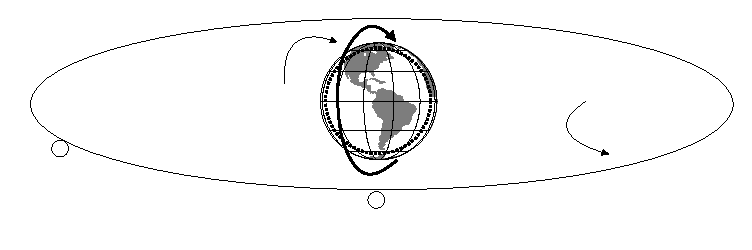
\includegraphics{figs/sats.fig.eps}%
\end{picture}%
\setlength{\unitlength}{4144sp}%
%
\begingroup\makeatletter\ifx\SetFigFontNFSS\undefined%
\gdef\SetFigFontNFSS#1#2#3#4#5{%
  \reset@font\fontsize{#1}{#2pt}%
  \fontfamily{#3}\fontseries{#4}\fontshape{#5}%
  \selectfont}%
\fi\endgroup%
\begin{picture}(5467,1641)(1921,-1651)
\put(1936,-1276){\makebox(0,0)[lb]{\smash{{\SetFigFontNFSS{10}{12.0}{\familydefault}{\mddefault}{\updefault}{\color[rgb]{0,0,0}GOES-West}%
}}}}
\put(4321,-1636){\makebox(0,0)[lb]{\smash{{\SetFigFontNFSS{10}{12.0}{\familydefault}{\mddefault}{\updefault}{\color[rgb]{0,0,0}GOES-East}%
}}}}
\put(3196,-691){\makebox(0,0)[lb]{\smash{{\SetFigFontNFSS{10}{12.0}{\familydefault}{\mddefault}{\updefault}{\color[rgb]{0,0,0}Polar-orbiting}%
}}}}
\put(5851,-556){\makebox(0,0)[lb]{\smash{{\SetFigFontNFSS{10}{12.0}{\familydefault}{\mddefault}{\updefault}{\color[rgb]{0,0,0}Geostationary}%
}}}}
\end{picture}%

  \caption{Satellite map showing \acs{GOES} orbits.}
  \label{fig:sats}
\end{figure}

\emph{Passive remote sensors} detect either reflected solar energy or
energy emitted from the surface itself.  \emph{Active remote sensors}
emit energy, typically radar or laser energy, and measure the
reflected energy from that source.  The \ac{GOES} satellites are
passive systems.

Table~\ref{tab:goes} gives an overview of the \ac{GOES} sensors.  The
satellite continuously scans a hemisphere of the Earth with two
sensors, the Imager and the Sounder.  The Imager acquires higher
resolution images in a limited number of bands, while the Sounder has
low resolution images, but with 19 bands designed for vertical
atmospheric profiling.  \ac{GOES}-West offers a continuous stream of
data for \acp{ROI} ranging from the continental United States to a
hemisphere centered near Hawaii at about $135^\circ$ West longitude.
\ac{GOES}-East is centered on the equator over South America, at about
$75^\circ$ West longitude.

\begin{table}[htb]
  \centering
  \caption{\ac{GOES} satellite sensors}
  \begin{minipage}[t]{2.5cm}
    \vspace*{0pt}
    
\includegraphics[width=2.5cm]{figs/motivation-goes.fig.eps}
  \end{minipage}
  \quad
  \begin{tabular}[t]{c | c}
    Imager & Sounder \\
    \hline \hline
    4 $[km^2]$ pixels & 64 $[km^2]$ pixels \\
    5 spectral bands &     19 spectral bands \\
    Data arrives by row(s) & Arrives by point \\
    1-8 rows at a time \\
    $[2,500-17,000]^2$ size \\
  \end{tabular}
  \label{tab:goes}
\end{table}

The current \ac{GOES} Imager is a five channel radiometer with one
spectral band in the visible region, two in the mid-infrared and two
thermal-infrared regions.  The passive radiometer senses reflected
solar energy in the visible, a combination of reflected and emitted
energy in the mid-infrared bands, and emitted energy from the Earth in
the thermal bands.

The \ac{GOES} Imager uses a telescope with a two-axis scanning mirror
at the entrance.  The mirror is moved using servos, which in turn scan
the hemisphere of the Earth.  The multi-spectral channels of the
Imager, simultaneously sweep an 8-kilometer swath on east-to-west and
west-to-east paths, at a rate of 20 degrees (optical) east-west per
second.  This means the Imager can scan a 3000 by 3000 km "box"
centered over the United States in about 41 seconds.  The scan takes
place by sweeping East to West, stepping the instrument South and
then scanning back West to East.

The imaging sensor, including the telescope, scan assembly, and
detectors, is located outside the main structure of the spacecraft.
Additional control electronics and power units are located internally
in the spacecraft.  Table~\ref{tab:imager} describes some of the
spectral characteristics of the \ac{GOES} Imager.  \acs{IGFOV} is the
\acf{IGFOV} directly below the instrument, at the nadir.
%
\begin{table}[htb]
  \centering
\caption{\ac{GOES} Imager characteristics}
  \begin{tabular}{>{\PBS\raggedright\hspace{0pt}}p{3cm}|c|c|c|c|c}
    Channel number & 1 (Visible) & 	2 (Shortwave) &	3 (H$_2$O) &	4 (IR 1) &	5 (IR 2) \\
    \hline \hline
    Wavelength [$\mu$m] & 0.55-0.75 &	3.80-4.00 &	6.50-7.00 &	10.20-11.20 &	11.50-12.50 \\ 
    Spectral Region & Visible & Shortwave &	Moisture &	TIR &	TIR \\
    IGFOV [km] 	&1&	4&	8 &	4 &	4 \\
%    Radiometric Accuracy &	5\% of max  & $\le 1$ K & $\le 1$ K & $\le 1$ K & $\le 1$ K \\ 
\end{tabular}
  \label{tab:imager}
\end{table}

The \ac{RSI} stream is continuous weather imagery from the \ac{NOAA}
\ac{GOES}~\cite{goes96databook}.  All data from the \ac{GOES}
satellite is transferred via a format specific to these instruments, the
\acf{GVAR} format. Figure~\ref{fig:gvar-stream} shows the
\ac{GVAR}~\cite{noaa00gvar-trans} data stream.

\begin{figure}[htb]
  \begin{center}
    \begin{picture}(0,0)%
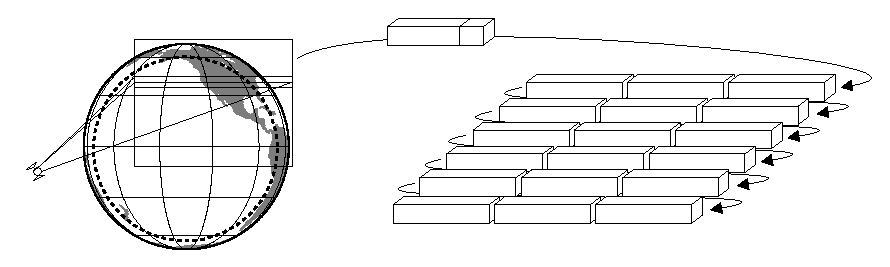
\includegraphics{figs/gvar.fig.eps}%
\end{picture}%
\setlength{\unitlength}{2072sp}%
%
\begingroup\makeatletter\ifx\SetFigFontNFSS\undefined%
\gdef\SetFigFontNFSS#1#2#3#4#5{%
  \reset@font\fontsize{#1}{#2pt}%
  \fontfamily{#3}\fontseries{#4}\fontshape{#5}%
  \selectfont}%
\fi\endgroup%
\begin{picture}(13032,3547)(2,-2716)
\put(5090,-2182){\makebox(0,0)[b]{\smash{{\SetFigFontNFSS{49}{58.8}{\sfdefault}{\mddefault}{\updefault}{\color[rgb]{0,0,0}...}%
}}}}
\put(8499,-357){\makebox(0,0)[b]{\smash{{\SetFigFontNFSS{6}{7.2}{\familydefault}{\mddefault}{\updefault}{\color[rgb]{0,0,0}IR (F,5)}%
}}}}
\put(10043,-357){\makebox(0,0)[b]{\smash{{\SetFigFontNFSS{6}{7.2}{\familydefault}{\mddefault}{\updefault}{\color[rgb]{0,0,0}IR (F,5)}%
}}}}
\put(11585,-357){\makebox(0,0)[b]{\smash{{\SetFigFontNFSS{6}{7.2}{\familydefault}{\mddefault}{\updefault}{\color[rgb]{0,0,0}Doc (F,5)}%
}}}}
\put(8095,-721){\makebox(0,0)[b]{\smash{{\SetFigFontNFSS{6}{7.2}{\familydefault}{\mddefault}{\updefault}{\color[rgb]{0,0,0}Vis (F,5)}%
}}}}
\put(9638,-721){\makebox(0,0)[b]{\smash{{\SetFigFontNFSS{6}{7.2}{\familydefault}{\mddefault}{\updefault}{\color[rgb]{0,0,0}Vis (F,5)}%
}}}}
\put(11179,-721){\makebox(0,0)[b]{\smash{{\SetFigFontNFSS{6}{7.2}{\familydefault}{\mddefault}{\updefault}{\color[rgb]{0,0,0}Vis (F,5)}%
}}}}
\put(7730,-1085){\makebox(0,0)[b]{\smash{{\SetFigFontNFSS{6}{7.2}{\familydefault}{\mddefault}{\updefault}{\color[rgb]{0,0,0}Sounder}%
}}}}
\put(9233,-1085){\makebox(0,0)[b]{\smash{{\SetFigFontNFSS{6}{7.2}{\familydefault}{\mddefault}{\updefault}{\color[rgb]{0,0,0}Auxillary}%
}}}}
\put(10814,-1085){\makebox(0,0)[b]{\smash{{\SetFigFontNFSS{6}{7.2}{\familydefault}{\mddefault}{\updefault}{\color[rgb]{0,0,0}No Data}%
}}}}
\put(7283,-1451){\makebox(0,0)[b]{\smash{{\SetFigFontNFSS{6}{7.2}{\familydefault}{\mddefault}{\updefault}{\color[rgb]{0,0,0}IR (G,5)}%
}}}}
\put(8824,-1451){\makebox(0,0)[b]{\smash{{\SetFigFontNFSS{6}{7.2}{\familydefault}{\mddefault}{\updefault}{\color[rgb]{0,0,0}IR (G,5)}%
}}}}
\put(10367,-1451){\makebox(0,0)[b]{\smash{{\SetFigFontNFSS{6}{7.2}{\familydefault}{\mddefault}{\updefault}{\color[rgb]{0,0,0}Doc (G,5)}%
}}}}
\put(6876,-1818){\makebox(0,0)[b]{\smash{{\SetFigFontNFSS{6}{7.2}{\familydefault}{\mddefault}{\updefault}{\color[rgb]{0,0,0}Vis (G,5)}%
}}}}
\put(8420,-1818){\makebox(0,0)[b]{\smash{{\SetFigFontNFSS{6}{7.2}{\familydefault}{\mddefault}{\updefault}{\color[rgb]{0,0,0}Vis (G,5)}%
}}}}
\put(9961,-1818){\makebox(0,0)[b]{\smash{{\SetFigFontNFSS{6}{7.2}{\familydefault}{\mddefault}{\updefault}{\color[rgb]{0,0,0}Vis (G,5)}%
}}}}
\put(6469,-2222){\makebox(0,0)[b]{\smash{{\SetFigFontNFSS{6}{7.2}{\familydefault}{\mddefault}{\updefault}{\color[rgb]{0,0,0}Doc (H,5)}%
}}}}
\put(8053,-2222){\makebox(0,0)[b]{\smash{{\SetFigFontNFSS{6}{7.2}{\familydefault}{\mddefault}{\updefault}{\color[rgb]{0,0,0}No Data}%
}}}}
\put(9557,-2222){\makebox(0,0)[b]{\smash{{\SetFigFontNFSS{6}{7.2}{\familydefault}{\mddefault}{\updefault}{\color[rgb]{0,0,0}Auxillary}%
}}}}
\put(6919,496){\makebox(0,0)[b]{\smash{{\SetFigFontNFSS{6}{7.2}{\familydefault}{\mddefault}{\updefault}{\color[rgb]{0,0,0}hdr}%
}}}}
\put(6227,496){\makebox(0,0)[b]{\smash{{\SetFigFontNFSS{6}{7.2}{\familydefault}{\mddefault}{\updefault}{\color[rgb]{0,0,0}data}%
}}}}
\put(6469,212){\makebox(0,0)[b]{\smash{{\SetFigFontNFSS{6}{7.2}{\familydefault}{\mddefault}{\updefault}{\color[rgb]{0,0,0}Data Blocks}%
}}}}
\put(3750,578){\makebox(0,0)[b]{\smash{{\SetFigFontNFSS{6}{7.2}{\familydefault}{\mddefault}{\updefault}{\color[rgb]{0,0,0}Frame 5}%
}}}}
\put(301,-1858){\makebox(0,0)[b]{\smash{{\SetFigFontNFSS{6}{7.2}{\familydefault}{\mddefault}{\updefault}{\color[rgb]{0,0,0}GOES}%
}}}}
\put(4604,-315){\makebox(0,0)[b]{\smash{{\SetFigFontNFSS{6}{7.2}{\familydefault}{\mddefault}{\updefault}{\color[rgb]{0,0,0}Scan G}%
}}}}
\put(4604,-155){\makebox(0,0)[b]{\smash{{\SetFigFontNFSS{6}{7.2}{\familydefault}{\mddefault}{\updefault}{\color[rgb]{0,0,0}Scan F}%
}}}}
\end{picture}%

%    \includegraphics[width=1\textwidth]{gvar.eps}
    \caption{GOES GVAR data stream}
    \label{fig:gvar-stream}
  \end{center}
\end{figure}

The \ac{GVAR} stream transmits at approximately 2.1 Mb/sec.  A frame
varies in size from about 100MB to 400MB, depending on the size of the
region scanned.  The footprint of an Imager pixel varies between
spectral channels.  Individual frames are made up of a large number of
scans which are narrow swathes of data corresponding to the physical
sweep of the instrument sensors from East to West.  The scans
themselves are made up of blocks of data, which are the atomic unit of
transfer from the satellite to the receivers.  Blocks contain from 32K
to 229K bits of data, depending on the width of the scan.  \ac{GOES}
visible channel data blocks contain 8 rows of data.  Other channels
from the \ac{GOES} Imager come in blocks of 1 or 2 rows.  The number
of columns in a row varies from frame to frame.  An entire frame of
data is reported 8 rows at a time from North to South.  New frames
start from their most Northern extents.

Documentation blocks include operational parameters, such as the
current location of the satellite, the current frame and scan,
parameters for each instrument, and additional information for each
spectral channel.


\subsection{Geolibraries}
\label{sec:geolibraries}

The first, and still most important role of databases in relation to
\ac{RSI}, is not to manipulate the images but instead to catalog what
images exist for what times and locations and organize this
information for users and producers.

As expected, geospatial libraries were not an important area of
research until warranted by the volume of available data.  Through the
1970's and even into the early 1990's, the limited number of data
providers and the method of data distribution, usually via computer
tapes, limited the need for sophisticated interfaces to repositories
of digital \ac{RSI} data.  More and more satellite instruments,
coupled with the advance of the \ac{WWW} have driven the need for more
advanced methods of access to \ac{RSI} archives.

In 1993, the \ac{NRC}, anticipating the need for coordination of
National spatial data envisioned the \acf{NSDI}:

\emph{ The National Spatial Data Infrastructure is the means to
  assemble geographic information that describes the arrangement and
  attributes of features and phenomena on the Earth. The
  infrastructure includes the materials, technology, and people
  necessary to acquire, process, store, and distribute such
  information to meet a wide variety of
  needs~\cite{nrc93towar-coord}.}

This led in 1994 to the founding of the
\acf{NSDI}~\cite{fed12906}, by executive order, to establish
technologies and standards necessary to encourage the use and sharing
of geospatial data within a number of communities, including
government, academia, and the private and non-profit sectors.  Goals
of the program include reducing costs and duplication and improve the
quality of geographic information.  \ac{NSDI} committees have developed a
number of standards covering the content standards for various
geographical data, transfer formats, spatial accuracy, and location
grids.  Perhaps the most important standard from the \ac{NSDI} is the
\acf{CSDGM}~\cite{fgdc98conten-stand}.  This standard describes the
required metadata that should be associated with any \ac{GIS} data
product.  It is used as a base record for many geospatial library
organization structures.

In 1998, the \ac{NRC} revisited the need for geospatial
libraries~\cite{nrc98distr-geolib}.  One of the main reasons for
this was that the original studies did not anticipate the profound
impact that the \ac{WWW} has had on data distribution and distributed
systems.  The panel argued the need for a common vision among
geolibraries, and put forth 15 major findings, pointing toward the
need for distributed systems based on \ac{WWW} services.  The \ac{NRC}
defined a geolibrary:

\emph{ A geolibrary is a digital library filled with geoinformation
  and for which the primary search mechanism is place. Geoinformation
  is information associated with a distinct area or footprint on the
  Earth's surface. A geolibrary is distributed if its users, services,
  metadata, and information assets can be integrated among many
  distinct locations.}

Of particular interest were the extensions in service that the
\ac{NRC} anticipated for these repositories.

\emph{ Finding 8: A distributed geolibrary would allow users to
  specify a requirement, search across the resources of the Internet
  for suitable geoinformation, assess the fitness of that information
  for use, retrieve and integrate it with other information, and
  perform various forms of manipulation and analysis. A distributed
  geolibrary would thus integrate the functions of browsing the WWW
  with those of GIS and related technologies.}

Today, there are many more examples of working geolibraries.  Both the
\ac{USGS} and \ac{NASA} offer exceptional geospatial data
libraries.  \ac{NASA}'s satellite data is made available via the
\acf{DAAC}~\cite{nasa06goddar-distr}, which offers access to data
products with multiple search interfaces and download capabilities.

\ac{USGS} makes all maps and imagery available through several sites
including the Earth Explorer~\cite{usgsearth-explor} and the Seamless
Data Distribution System~\cite{usgsseaml-data-distr-system}.  These
services all provide many of the required features of a geolibrary,
typically over a single repository, however.  Queries working over
distributed, heterogeneous databases, is still an important need in
the \ac{GIS} community.

\subsection{Standards}

Standards fulfill an important role in making data products most
useful to the widest audience.  Just as the early days of remote
sensing did not need common methodologies for description and
discovery, many data products developed their own specific data
formats.  Early image formats, still quite popular today, were very
simple binary representations of the image pixels.  Additional
information is included in separate files for inside image headers.
In recent years, various standards have been introduced into the
\ac{GIS} landscape, and have been widely adapted in many applications.
Two examples include the \ac{ESRI} Shapefile for vector data and the
GeoTIFF standard for images.  The Shapefile
format~\cite{esri97esri-shapef-techn-descr} describes points, lines,
or polygons, along with associated attributes of the items.  There is
also a specification for an attached R-tree based index structure, and
a coordinate space.  The GeoTIFF
specification~\cite{ritter00geotif-format}, published in 2000, is an
extension of the TIFF standard that embeds metadata relating to
georeferencing information within the file itself.  Both standards
have become very popular because they are relatively simple and
effective formats that have grown into standards having proved their
utility in multiple applications.  These types of formats have
typically succeeded far better than formats developed from whole cloth
by committee, the Spatial Data Transfer
Standard~\cite{spatial-data-trans-stand}.  The GeoTIFF format is the
de facto standard for remotely sensed imagery, although there are
many, many formats in active use~\cite{wiki06}.

Some standards organizations, however, have been very successful in
encouraging \ac{GIS} standards, none so more than the \acf{OGC}.  The
\ac{OGC} is a consensus based organization, consisting of members from
government, academia, and commercial
fields~\cite{06open-geosp-consor}.  The \ac{OGC} has been especially
effective in developing interoperability standards for Internet and
web-based scenarios:

\begin{itemize}
\item The \ac{OGC} Abstract Specification is the conceptual foundation for
most \ac{OGC} specification development activities and provides a
reference model for the development of implementation specifications.

\item Coordinate systems are defined with a
\acf{WKT}~\cite{whites01defin-data} representation, used in most
\ac{OGC} specifications.

\item The \acf{GML} is an \ac{XML} grammar for the modeling, transport, and
storage of geographic information, providing objects for describing
geography including features, geometry, topology, time, units of
measure and generalized values.

\item The \acf{WMS} and \acf{WCS} specifications allow clients to retrieve
map images for display or to provide a network interchange of
geo-spatial image data through a standard query mechanism.

\end{itemize}

The \ac{OGC} is also a major force in the creation of the \acf{ISO},
in particular the ISO/TC 211~\cite{iso-tc} technical committee on
geographic information and geomatics.  The \ac{ISO} 19100 series of
standards are incorporating the \ac{OGC} abstract specification, and a
number of other \ac{OGC} specifications are or will be adopted by
\ac{ISO}/TC 211~\cite{wiki06}.


\subsection{Geospatial Databases}

Geospatial databases typically differ from geolibraries in that the
focus is on manipulation of spatial data, as opposed to
archival and retrieval.  As discussed in
Section~\ref{sec:geolibraries}, this distinction is becoming somewhat
artificial as geolibraries expand their services.  Most geolibraries
use geospatial database backends.

There are many sources of information on the particulars of
geospatial databases.  G\"uting~\cite{gutin94introd-spatial} and
Rigaux~\cite{rigaux02spatial-datab} both include comprehensive
introductions to the terminology of these systems.  The
material below was distilled in large part from this introductory
material.  

A \emph{geospatial database} is a database that can store and describe
\emph{geographic objects}.  Geographic objects within the database
have a \emph{geometric attribute} or \emph{spatial extent}, which can
describe in some manner the location, size and shape of an object.
This description may be in two or three dimensions.  Geospatial
databases include extents that correspond to actual physical
locations.  There exists a mapping of the object's extent to an actual
place.  In addition to a spatial attribute, geographic objects may
also have non-spatial or descriptive attributes.  A \acf{SDBMS} allows
access to the objects based on either their spatial or non-spatial
attributes, or some combination of attributes.  It is the geometric
attribute of objects that is the defining feature of a \ac{SDBMS}.
For example, satellite images could be stored in an \emph{image
  database}, where the focus might be on manipulating images based on
the content of the images, rather than their location.

\emph{Spatio-temporal} databases describe objects in both a spatial
and a temporal manner.  How objects are described in time, either as
an additional dimension, a trajectory, a set of historical locations,
or some other method, varies by their requirements and implementation
and constitute an on-going research area.

One method of dividing what phenomena can be described by a spatial
database is whether the model is \emph{entity-based} or
\emph{field-based}.  In an entity-based model, objects include
descriptive characteristics and a geographic attribute.  The
geographic attribute defines a number of points in space that make up
that object.  A representation of countries would be a good candidate
for entity-based objects, where an individual country has a number of
descriptive attributes along with an geographic attribute that defines
the boundaries of the country.  In \emph{field-based} models,
attributes are not associated with individual objects.  Rather,
attribute are considered as functions over some spatial domain and
there exists one attribute value associated with any point in space.
Images are field-based models.  The system defined in this paper is
predominantly field-based, although some aspects, like query
\acp{ROI}, are entity-based.

Entity-based models can use \emph{Tessellations}~\cite{wiki06} to
partition a space into a discrete set of cells.  These cells are
usually regular grids, but could be other structures like hexagons, or
irregular triangular or polygonal separations.  In these models the
actual extent is approximated by an integral set of tessellation
cells.  These cells can be referenced directly, or a further
decomposition, for example, a quad tree, might be used to minimize the
description of the tessellation.  Field-based data is also well
represented with tessellations, with a modification that the attribute
function is no longer defined on a continuous spatial domain, but
instead on the discrete areas corresponding to the tessellation cells.
All satellite imagery, in fact, all imagery in this research uses a
point set definition that implies an associated tessellation of the
underlying spatio-temporal space.


\section{Data Stream Management Systems}
\label{sec:dsms}


Most research on querying and managing data streams has concentrated
on either traditional data models where the data arrives in the form
of simple records (tuples) or XML data.  Several overviews on the
recent advancements in \acl{DSMS} have been
published~\cite{babcoc02model-issues, carney02monit-stream,
  heller00adapt-query}. In such systems, data arrives in multiple,
continuous, and time-varying data streams and does not take the form
of persistent relations.  The current interest in data stream
management ~\cite{abadi03auror,babcoc02model-issues,chand03teleg} has
driven various new processing methods and paradigms for streaming
data, such as
adaptivity~\cite{heller00adapt-query,madden02contin-adapt}, operator
scheduling ~\cite{babcock04op,carney03operat-sched}, and load shedding
~\cite{babcock04load,tatbul03load}.  Some proposed approaches have
extended to the realm of spatio-temporal databases as well, where new
methods defining the spatial relationships between queries and data
streams are being investigated, in particular in the context of
continuous queries over moving objects (e.g.,
~\cite{kalas04main-memor,mokbel04sina,prabhakar02qindex}).
%  Research into
%where these new streaming data paradigms can have a great impact in
%applications surrounding remotely sensed geospatial image data
%originating from various satellites orbiting the Earth.

Formalisms on streaming databases are described by Arasu, Babcock,
Motwani and Widom~\cite{arasu03cql-contin, babcoc02model-issues,
  motwan03query-proces} and realized in the Stanford STREAM project,
which has a goal of producing a general purpose \ac{DSMS} that adds
data streams into a \ac{DBMS} in a coherent and consistent
manner~\cite{arasu03stream}.

Additional implementations of \ac{DSMS} include
Telegraph~\cite{chand03teleg}, based in part on
Postgresql~\cite{stonebraker90implementation}.  In Telegraph, all
continuous queries are optimized with postgresql and executed with an
eddy based routing to operators~\cite{madden02contin-adapt}.

PSoup~\cite{950486} extends some of Telegraph's processing
architecture to allow retrospective queries on data that was
previously received.  PSoup regards multi-query processing as a join
of both query and data streams.

Aurora~\cite{abadi03auror} is another \ac{DSMS} that optimizes and
executes queries in a process oriented, dataflow paradigm.  Rather
than using a declarative query interface, Aurora allows users to
stitch together a stream-oriented process.

There are currently several research efforts in the context of
\ac{DSMS} that focus on core issues such as adaptive query processing
~\cite{chen02desig-evaluat, madden02fjord-stream,
  madden02contin-adapt,shah03flux}, meaning and implementation of
blocking operators, including aggregation and sorting
~\cite{haas99rippl-joins,luo02scalable}, and approximate query
processing techniques ~\cite{dobra02proces,gehrk01comput-correl}.
Specific implementations of specialized optimizations include adaptive
strategies to continually modify tuple processing~\cite{avnur00eddies,
  heller00adapt-query, madden02fjord-stream, madden02contin-adapt}.

Streaming spatio-temporal data has primarily been investigated in the
context of moving objects and location-aware services.  Query
processing and optimization aspects for streaming \acf{RSI} data are
quite different. Streaming \acs{RSI} is typical for the vast amount of
imaging satellites orbiting the Earth and it exhibits certain
characteristics that make it very attractive to tailored query
optimization techniques.

Optimizing streaming databases has many similarities with methods for
optimizing multi-queries in traditional databases,
Sellis~\cite{sellis90multip-query} offering some of the earliest
examples for finding common sub-expressions.  Other studies for
multi-query optimizations through common sub-expressions
include~\cite{graef93volcan-optim,pellen97compl-trans,roy00effic}.


Figure~\ref{fig:overview} (page \pageref{fig:overview}) showed an
overview of a \acf{DSMS} for \acf{RSI} data.  Such data have a number
of characteristics that are different from the typical streaming
relational or spatio-temporal data typically described in a \acs{DSMS}
context.  One aspect is that the incoming bandwidth of \acs{RSI} data
streams is very large, usually arriving as discrete parts of binary
image data.  Another important point is that streaming \acs{RSI} data
is more highly organized with respect to its spatial and temporal
components than is usually assumed for more generic types of
spatio-temporal data.  This organization effects how data and queries
can be processed in a \ac{RSI} \acs{DSMS}.  These aspects are
described in Section~\ref{sec:point-sets} and Chapter~\ref{cha:query}.


\chapter{The \ac{GS} Model}
\label{cha:models}

Developing efficient optimization strategies for streaming \ac{RSI}
data requires a consistent and practical model describing the \ac{RSI}
data stream, the queries made to the system, and the operations that
are performed on the stream to answer those queries.

The models developed here begin with some preliminary definitions of
images and image operations, based in image algebra.  From this
foundation, some additional definitions specific to the \ac{GS}
project are introduced to define a data model defining images and
image operations.  Image algebra provides an underlying framework for
manipulating images.  However, in order to be used effectively for
geospatial images in the streaming context of a \ac{DSMS}, aspects
specific to this application need to be addressed.  These changes are
discussed in Section~\ref{sec:dm}.  Some modifications are also
required on certain operators to more easily allow for point sets of
indeterminate length, as required for a \ac{DSMS}.

The query model is introduced in Section~\ref{sec:qm}.  Although
queries are basically image algebra expressions resulting in images,
some additional information on the formulation of queries is defined.
This includes the adoption of a simple syntax using the \acf{WMS}
interface.  One major feature of an effective query processor is
choosing an optimal execution plan for a given query.  Because queries
are in image algebra, specialized rules regarding the rewriting of
image algebra expressions are introduced.

\section{Image Algebra Definitions}
\label{sec:image-algebra}

An image has a fairly intuitive definition, but a more formal
definition is required for the purposes of developing a consistent
method describing operations on images.  Image algebra is a unified
theory for image transformation and analysis.  It is a many-valued
algebra, with multiple operators and operands.  Images consist of sets
of points and values associated with these points.  Image
algebra includes \emph{Point Sets}, \emph{Value Sets}, and
\emph{Images}.

\emph{A {\bf point set} is simply a space.  Individual elements of the
  set are called {\bf points}.}  Common point sets used in image
algebra include discrete subsets of an $n$-dimensional Euclidean space
$\vs{R}^n$.  Some important subsets include integer points, $\vs{Z}$,
and $n$-dimensional point lattices, $\vs{Z}^n$.

\emph{A {\bf point lattice } is a regularly spaced grid of points.}
Images corresponding to \ac{RSI} datasets defined in this research all
have square lattices on an integer point space as their point sets.
Points in the image space are correlated with a real world locations
through associations with a well defined projection system and a
matrix transformation to that coordinate space
(Section~\ref{sec:point-sets}).  Point sets are denoted with bold
capital letters, i.e., \ps{X}, \ps{Y}, \ps{Z}.  Points within a point
set are denoted with lower case bold letters, i.e., $\pt{y} \in
\ps{X}$.
%When the point set is a
%point lattice, the points inherit vector space operations and standard
%$n$-dimensional point operations apply, i.e, $\im{x}+\im{y} =
%(x_1+y_1,x_2+y_2,\ldots,x_n+y_n)$.


\emph{A {\bf value set} is a set and the associated operations among
  members of that set.  Members of the set are called {\bf values}.}
Value sets simply contain all the potential values associated with
points in a single image.  Typical value sets include integers,
$\vs{Z}$ and real numbers, $\vs{R}$.  These value sets have the usual
operations associated with their particular set.  Value sets are
denoted as capital letters in blackboard font like $\vs{V}$.

\emph{{\bf Images} are functions mapping points to values, or as a set
  of point value pairs.  These individual pairs are the \emph{pixels}
  in the image.}

The notation $\imType{V}{X}$ describes the set of all functions, $f
\in \imType{V}{X}: f \text{ is a function } \ps{X} \rightarrow \vs{V}$.
An image is such a function that maps from a point set \ps{X} to the
value set \vs{V}.  For an \vs{V}-valued image, ($\im{a}: \im{X} \to
\vs{V}$), \vs{V} is the possible {\bf range} of the image \im{a}, and
\ps{X} is the {\bf domain} of \im{a}.

Another convenient notation for an image $\im{a} \in \imType{V}{X}$ is
the {\bf graph } or {\bf data structure } representation, $\im{a} =
\{(\pt{x},a(\pt{x}) : \pt{x} \in \ps{X}\}$.  Here the pair
$(\pt{x},a(\pt{x}))$ constitutes a {\bf pixel} of the image.  The
first coordinate $\pt{x} \in \ps{X}$ is the {\bf pixel location} and
the second coordinate $a(\pt{x}) \in \vs{V}$ is the {\bf pixel
  value} at location \pt{x}.

There are a number of operations on images that are required to answer
the queries submitted to the system.  The four most important
operations are composition, induced operation, restriction, and
neighborhood operation.  These are shown in the notional diagram of
Figure~\ref{fig:ops}, and discussed below.

 \begin{figure}[htb]
  \centering
 \subfigure[Composition]{
   \begin{pspicture}(2,2)
       {\psset{unit=0.3}\extent(0,0)(6,6)}
      \SpecialCoor
      \newpsstyle{pc}{fillstyle=solid,fillcolor=white,linecolor=lightgray,origin={2,-1.8}}
      \pspolygon[style=pc](2;0)(4;0)(4;-24)(2;-24)(2;0)
      \psline[style=pc](2;-6)(4;-6)
      \psline[style=pc](2;-12)(4;-12)
      \psline[style=pc](2;-18)(4;-18)
      \psline[style=pc](2.5;0)(2.5;-24)
      \psline[style=pc](3;0)(3;-24)
      \psline[style=pc](3.5;0)(3.5;-24)
     \pscurve[doubleline=true]{->}(0.1,0.1)(.2,.7)(.5,.9)
      \end{pspicture}
 }\quad
 \subfigure[Induced operation] {
   \psset{unit=0.3}
   \begin{pspicture}(10,10)
     \extent(0,0)(4,4)
     \roi(0,0)(4,4){$\im{a}$}
     \extent(0,6)(4,10)
     \roi(0,6)(4,10){$\im{b}$}
     \extent(6,3)(10,7)
     \roi(6,3)(10,7){$\im{a}\gamma\im{b}$}
     \pscurve[doubleline=true]{->}(0.5,3.5)(6,5.5)(6.5,6.5)
     \pscurve[doubleline=true]{->}(0.5,9.5)(5,9.5)(6.5,6.5)
   \end{pspicture}
 }\quad
 \subfigure[Restriction]{
   \psset{unit=0.3}
   \begin{FramePic}[10,10]
     \roi(2,2)(7,7){$\ps{X}$}
   \end{FramePic}
 }\quad
 \subfigure[Neighborhood]{
   \psset{unit=0.3}
   \begin{pspicture}(10,10)
     \extent(0,0)(6,6)
     \roi(0,0)(3,3){}
     \extent(4,4)(10,10)
     \roi(4,4)(10,10){}
     \roi(5,5)(6,6){}
     \pscurve[doubleline=true]{->}(1.5,1.5)(3,2)(5.5,5,5)
   \end{pspicture}
 }
 \caption{Image algebra operations}
 \label{fig:ops}
\end{figure} 

Since images are defined as functions, standard functional operations
apply as well.  \emph{A {\bf composition} is the nesting of two or
  more functions to form a single new function.}  There are two orders
on the nesting of the functions.

Given a function $\Gamma:\vs{V}\to\vs{W}$, the composition, or value
transform, $\Gamma\circ\im{a}$, changes an image in \imType{V}{X} to
an image in \imType{W}{X} defined as:\[
\Gamma\circ\im{a} \equiv \Gamma(\im{a})=\{(\pt{x},\Gamma(a(\pt{x}))) : \pt{x}\in\ps{X}\}\]

Given a function $f:\ps{Y}\to\ps{X}$ between two point sets, the
composition, or spatial transform, $\im{a}\circ f$, changes an image
$\im{a}\in \imType{V}{X}$ from \imType{V}{X} to \imType{V}{Y}
where \[\im{a}\circ f \equiv \{(\pt{y},a(f(\pt{y})) : \pt{y}\in\ps{Y}\}\]

The composition $\Gamma\circ\im{a}$, can be used to define operations
on the values of an image.  A natural set of induced operations on
images are defined. \emph{Any operation that operates on the value set
  \vs{V}, defines a natural {\bf induced operation} on \vs{V}-valued
  images.}  If $\gamma$ is some binary operation on \vs{V}, then for
$\im{a_1},\im{a_2} \in \imType{V}{X},
\im{a_1}\gamma\im{a_2}=\{(\pt{x},\gamma(a_1(\pt{x}),a_2(\pt{x}))) :
\pt{x}\in\ps{X}\}$.  If $\gamma()$ is an $n$-valued operation on
values $v_1,v_2,\ldots,v_n$, then $\gamma(a_1,a_2,\ldots,a_n)$ is a
similarly defined induced operation.

The functional composition, $\im{a}\circ f$, where $f$ is applied to
the image point set is often used to project images to new geographic
coordinate systems.  For consistency to other \ac{RSI} frameworks,
these will be described as spatial transformations as they map an
image from one point set to another.  Note that the definition of a
spatial transform implies that the image is defined for an arbitrary
point located at $f(\pt{y})$.  Section~\ref{sec:trans-op}, describes
how an \ac{RSI} image may be defined on arbitrary points by, for
example, interpolation methods on the original image.

Other basic concepts of function theory can be applied to images.  In
addition to the previously described domain, range and
composition, these include \emph{restriction} and
\emph{extension} operators.  Restrictions can be defined on both the
point set and the value set of an image.

If $\im{a}\in\imType{V}{X}$, then \emph{the {\bf point restriction}, $a|_Z$ of
\im{a} to a subset $\ps{Z} \subseteq \ps{X}$, is defined as
\[\im{a}|_\ps{Z}\equiv\im{a} \cap ( \ps{Z} \times \vs{V} ) =\{(\pt{x},a(\pt{x})): \pt{x}\in\ps{Z}\}
\]}

If $\im{a} \in \imType{V}{X}$, then \emph{the {\bf value restriction},
$a\|_\vs{S}$ of \im{a} to a subset $\vs{S} \subseteq \vs{V}$ is defined as:
\[\im{a}||_\vs{S}\equiv\im{a}\cap (\ps{X}\times\vs{S}) =\{(\pt{x},a(\pt{x})): \pt{x} \in \ps{X}, a(\pt{x}) \in \vs{S}\}\]}

The query model makes extensive use of the restriction operator.  This
is the primary mechanism to create image subsets that satisfy requests
for the specific \acf{ROI} for a query.  The extension of an image,
\im{a}, can extend the image to an expanded point set beyond the
original space of the image.  By defining a function, \im{b},
extensions can be used to grow images to expanded domains.

\emph{The {\bf extension} of $\im{a} \in \imType{V}{X}$ to
  $\im{b} \in \imType{V}{Y}$, where \ps{X} and \ps{Y} are subsets of
  the point set \ps{Z} is defined as:
\[
    \im{a}|^{\im{b}}(\pt{x}) =
    \begin{cases}
      a(\pt{x}) & \text{ if $\pt{x} \in \ps{X}$ } \\
      b(\pt{x}) & \text{ if $\pt{x} \in \ps{Y} \setminus \ps{X} $ }      
    \end{cases}
\]}

Although the extension operator is not included explicitly in the
query model below, refined models could use this to
allow users to choose some additional parameters on queries.  This is
discussed in more detail in Section~\ref{sec:restriction-types}.

Finally, \emph{{\bf neighborhood operations} allow for multiple pixels
  from a single image to be combined to create a single pixel in
  a new image.}  Although the neighborhood operation is conceptually
simple, its definition is somewhat convoluted.  For the summation
operation of neighborhood $\im{n}$ over image \im{a}

\[\im{a} \oplus \im{n}= \sum_{\parbox{1.5cm}{$\pt{y}\in\ps{Y}\vspace*{-10pt}\\  \pt{x}\in n(\pt{y})$}} a(\pt{x})\]

Where the image \im{n} has a point set, \ps{Y}, and each value of
\im{n} is itself a point set, $\ps{X'} \subset \ps{X}$.  For every
point $\pt{y} \in \ps{Y}$, \im{n} describes a set of points whose
values will be aggregated.  Typically, the points sets $\ps{X'}$ are
small uniform regions around a single point, the $3\times 3$ grid shown in
Figure~\ref{fig:ops} for example.

Neighborhood operations are used for averaging satellite images into
lower resolution pixels.  Users often desire images at a coarser
resolution than the raw satellite data when investigating or modeling
large areas.  The goal of the neighborhood operation is to model what
the radiance of \ac{RSI} image would be if it were acquired at this
coarser scale.  No methodology can replicate this goal exactly,
primarily because, in general, the final point sets do not align
exactly with the boundaries in the original image point set.  This is
especially true with queries in different coordinate systems, where
the resolution for a point set transformed to the \ac{GOES} reference
frame is not even necessarily constant.

Section~\ref{sec:qm} will show how all the operations can be combined
to allow for the specification of queries against the
\ac{RSI} data stream in the \ac{GS} environment.  First, however, the
image algebra formulations require some modifications for use with
streaming image data.

\section{Data Model}
\label{sec:dm}

The image algebra definitions above go a long way toward a definition
of a complete data model.  However, a few modifications and extensions
to the model need to be included to cover some aspects particular to
\acf{RSI}.  The aspects include additional features to reference image
point sets to real world locations and an explicit ordering associated
with the points in a point set.  This ordering allows operations to
execute on the incoming data stream.  These modifications lead to the
definition of a \ac{GS} image.  In addition, the ordering of the point
set allows a streaming image to be broken down into smaller images.
Two special subsets, the frame and row, will be explicitly defined.  A
single row of data will be the atomic element passed among operators
during query execution.  Rows, images, and frames are the primary
components of a reference schema for the data streams in the system.

\subsection{Streaming Geographic Point Sets}
\label{sec:point-sets}

In order to support streaming geospatial images, the definition of a
point set needs to be modified to explicitly include a frame of
reference for the point sets corresponding to Earth coordinates, and
to include an explicit ordering on the points.  These modifications
allow for images to be compared in terms of their underlying
geographic coordinate system and for operations to proceed on
streaming \ac{RSI} data.

\ac{GS} queries on the \ac{RSI} data either explicitly or implicitly
reference a particular coordinate system.  However, the physical
representation of the images are in a simple grid space.  To provide a
transformation between these two spaces, point sets need parameters
that describe the translation between the raster and model coordinate
systems.  The implementation used in the \ac{GS} system represents
this transformation with two parameters, the \emph{projection
  definition} and the \emph{matrix transformation}.  This
representation is similar to the representation of the \ac{OGC}
\ac{GML} standard~\cite{cox03geogr-markup, whites05recom-xml}.  It
also works well with the \ac{OGC} \ac{WMS} specification, which will be
the basis of \ac{GS} queries described in
Section~\ref{sec:wms-queries}.

The \emph{projection definition} is a standard representation
described by the \ac{OGC} \acf{WKT}~\cite{whites01defin-data}.  These
are text representations for all standard Earth projections.
Figure~\ref{fig:wkt} is an example of a complete definition of a
particular coordinate system.  The figure shows that each parameter in
the \ac{WKT} definition is assigned an authority and an identifier.
Some \ac{GIS} standards require that systems know all definitions of
certain authorities.  In that case, the identifiers alone can be used
as specifications.  In the case of Figure~\ref{fig:wkt}, the shorthand
notation of the projection definition is simply ``epsg:26941''.

\begin{figure}[htb]
  \centering
\begin{verbatim}
PROJCS["NAD83 / California zone 1",
  GEOGCS["NAD83",
         DATUM["North_American_Datum_1983",
               SPHEROID["GRS 1980",
                        6378137,
                        298.257222101,
                        AUTHORITY["EPSG","7019"]],
               AUTHORITY["EPSG","6269"]],
         PRIMEM["Greenwich",0,
                 AUTHORITY["EPSG","8901"]],
         UNIT["degree",0.01745329251994328,
              AUTHORITY["EPSG","9122"]],
         AUTHORITY["EPSG","4269"]],
  PROJECTION["Lambert_Conformal_Conic_2SP"],
  PARAMETER["standard_parallel_1",32],
  PARAMETER["standard_parallel_2",42],
  PARAMETER["latitude_of_origin",37.5],
  PARAMETER["central_meridian",-100],
  PARAMETER["false_easting",2000000],
  PARAMETER["false_northing",500000],
  UNIT["metre",1,
       AUTHORITY["EPSG","9001"]],
  AUTHORITY["EPSG","26941"]]
\end{verbatim}  
  \caption{\acs{OGC} \acs{WKT} definition, epsg:26941}
  \label{fig:wkt}
\end{figure}

The definition describes the PROJECTION, and all the details of the
associated \texttt{PARAMETER}s. The geographic coordinate system,
\texttt{GEOGCS}, is the most complex parameter, which includes the
\texttt{SPHEROID}, and \texttt{DATUM}, as well as the prime meridian.
Even without extensive knowledge of coordinate systems, the above
definition is readable.  This particular projection, ``California zone
1'', is in the Lambert conformal conic projections, with parameters;
standard parallels of 32 and 42, a latitude of origin at 37.5, and
central meridian at -100 degrees longitude, and so on.

By convention images are typically defined in a row/column coordinate
system, with the origin in the upper left hand corner of the image.
The method of converting these coordinates to a real world coordinate
system is by using a \emph{transformation matrix}.  This matrix
formulation allows for a general affine transformation between the
raster and model space.  The affine transform consists of six
coefficients that map row/column coordinates into the model space, as
shown in Figure~\ref{fig:affine}.  Consistent with many other \ac{GIS}
systems, \ac{GS} model simplifies this transformation and uses only
the scale and bias form of the transformation, where $s_x$ and $s_y$
are the scale factors, or length and width of an individual pixel, and
$b_x$ and $b_y$ correspond to the location of the upper left hand
image pixel in real world coordinates.  This is shown in
Figure~\ref{fig:scale}.

\begin{figure}[htb]
  \centering
  \subfigure[Affine transformation]{
      \label{fig:affine}
      \parbox[c]{2.3cm}{
        \begin{pspicture}(2,2)
          {\psset{unit=0.4}
            \extent(0,0)(4,4)
            \psline[linecolor=black]{->}(0,0)(4.2,0)
            \uput{8pt}[r](4,0){x}
            \psline[linecolor=black]{->}(0,0)(0,4.2)
            \uput{8pt}[u](0,4){y}
          }
        \end{pspicture}
      }
      \quad
        \parbox[c]{0.4\linewidth}{\small
          \centering
          \begin{equation*}
            \begin{bmatrix}x\\y\\1 \end{bmatrix} = 
            \begin{bmatrix}m_{11} & m_{12} & m_{13} \\ m_{21} & m_{22} & m_{23} \\ 0 & 0 &1
            \end{bmatrix}  \begin{bmatrix}u\\v\\1 \end{bmatrix}
          \end{equation*}
        }
      \quad
      \parbox[c]{2.3cm}{
        \begin{pspicture}(2,2)
          \SpecialCoor
          \newpsstyle{pc}{fillstyle=solid,fillcolor=white,linecolor=lightgray,origin={2,-1.8}}
          \pspolygon[style=pc](2;0)(4;0)(4;-24)(2;-24)(2;0)
          \psline[style=pc](2;-6)(4;-6)
          \psline[style=pc](2;-12)(4;-12)
          \psline[style=pc](2;-18)(4;-18)
          \psline[style=pc](2.5;0)(2.5;-24)
          \psline[style=pc](3;0)(3;-24)
          \psline[style=pc](3.5;0)(3.5;-24)
          \psline[origin={2,-1.8},linecolor=black]{->}(2;0)(4.1;0)
          % Remember origin
          \uput{8pt}[r](2.1,1.8){u}
          \psline[origin={2,-1.8},linecolor=black]{->}(2;0)(2;-30)
          \uput{8pt}[u](0,0){v}
        \end{pspicture}
      }
    }

    \subfigure[Bias and scale transformation]{
    \label{fig:scale}
    \parbox[c]{2.3cm}{
      \begin{pspicture}(2,2)
        {\psset{unit=0.4}
          \extent(0,0)(4,4)
          \psline[linecolor=black]{->}(0,0)(4.2,0)
          \uput{8pt}[r](4,0){x}
          \psline[linecolor=black]{->}(0,0)(0,4.2)
          \uput{8pt}[u](0,4){y}
        }
      \end{pspicture}
    }
    \quad
    \parbox[c]{0.3\linewidth}{\small
      \begin{equation*}
        \begin{bmatrix}x\\y\\1 \end{bmatrix} = 
        \begin{bmatrix}s_x & 0 & b_x \\ 0 & s_y & b_y \\ 0 & 0 &1
        \end{bmatrix}  \begin{bmatrix}u\\v\\1 \end{bmatrix}
      \end{equation*}
    }
    \quad
    \parbox[c]{2.3cm}{
      \begin{pspicture}(2,2)
        {
          \psset{xunit=0.3,yunit=0.4}
          \extent(0,0)(4,4)
          \psline[linecolor=black]{->}(0,4)(4.2,4)
          \uput{8pt}[r](4,4){u}
          \psline[linecolor=black]{->}(0,4)(0,-0.2)
          \uput{8pt}[d](0,0){v}
        }
      \end{pspicture}
    }
  }
  \caption{Image transformations}
  \label{fig:transformation}
\end{figure}

The streaming nature of the incoming \ac{RSI} imparts an ordering on
the points in the point set.  This ordering allows image operations to
proceed on the image stream, since it can be determined whether a
particular point will arrive.  It allows pixels from different images
to be aligned, and it allows for specialized organization of the data.
The point sets in the \ac{GS} system have a well defined ordering
associated with the set.

Point set orders depend on the remote sensing instrument. Different
instruments collect their data with different methods and impose
different structures on the points sets. For example, some instruments
have non-uniform point set structures and can only be ordered in time.
Sensors such as \ac{LIDAR}~\cite{kavaya99lidar-tutor}, which take
point measurements at discrete time steps, create such point sets.
Other instruments have an underlying point lattice for their images.
This gridded structure may have many points acquired at the same time,
but in this constant time the images have additional structure to
define a point set ordering.  Figure~\ref{fig:point-set} shows an
example of non-lattice and lattice point sets associated with
different image acquisition schemes.

\begin{figure}[htb]
  \centering
  \subfigure[Non-uniform point set]{
    \label{fig:ns-non}
    \psset{unit=0.4}
    \begin{pspicture}(10,10)
        \pscurve[fillstyle=none,linecolor=gray,dotstyle=square,dotsize=12pt,showpoints=true]{->}%
        (1.4,1.5)(1.6,2.6)(1.5,3.7)(1.5,4.8)(1.3,5.9)(1.5,7.0)(1.6,8.2)(1.7,9.3) %
        (3.2,9.5)(3.0,8.6)(3.0,7.4)(2.9,6.5)(2.8,4.5)(2.6,3.5)(2.8,2.5)(3.2,1.5)%
        (4.4,1.5)(4.6,2.6)(4.5,3.7)(4.5,4.8)(4.3,5.9)(4.5,7.0)(4.6,8.2)(4.7,9.3) %
        (6.2,9.5)(6.0,8.6)(6.0,7.4)(5.9,6.5)(5.6,5.5)(5.8,2.5)(6.2,1.5)%
        (8.2,1.3)(8.5,2.1)(8.5,3.4)(8.6,4.5)(8.4,5.3)(8.3,7.4)(8.4,8.8)
        \pscurve[fillstyle=none,linecolor=gray,dotstyle=square,dotsize=12pt,showpoints=false]{->}%
        (1.4,1.5)(1.6,2.6)(1.5,3.7)(1.5,4.8)(1.3,5.9)(1.5,7.0)(1.6,8.2)(1.7,9.3) %
        (3.2,9.5)(3.0,8.6)(3.0,7.4)(2.9,6.5)(2.8,4.5)(2.6,3.5)(2.8,2.5)(3.2,1.5)%
        (4.4,1.5)(4.6,2.6)(4.5,3.7)(4.5,4.8)(4.3,5.9)(4.5,7.0)(4.6,8.2)(4.7,9.3) %
        (6.2,9.5)(6.0,8.6)(6.0,7.4)(5.9,6.5)(5.6,5.5)(5.8,2.5)(6.2,1.5)%
        (8.2,1.3)(8.5,2.1)(8.5,3.4)(8.6,4.5)(8.4,5.3)(8.3,7.4)(8.4,8.8)
    \end{pspicture}
  }
  \subfigure[Point lattice] {
    \label{fig:ns-lat}
    \psset{unit=0.4}
    \begin{FramePic}[10,10]
   \end{FramePic}
}
\caption{Different point set types}
\label{fig:point-set}
\end{figure}

Even for sensors delivering images on point lattices, exactly how data
arrives with respect to time varies for different \acs{RSI} data
streams.  Image data generally arrives as discrete contiguous packets
of data.  The packets may be individual pixels or organized sets of
pixel data, depending on the instrument.  Figure~\ref{fig:lattice}
illustrates some common pixel organizations; image-by-image,
row-by-row, and pixel-by-pixel.  

 \begin{figure}[htb]
   \centering
   {
     \psset{unit=0.3} 
     \newpsobject{cover}{psframe}{linecolor=white,fillstyle=solid,fillcolor=white,linewidth=1pt}
     \newpsobject{pointset}{psgrid}{gridcolor=lightgray,subgriddiv=0,gridlabels=0,gridwidth=0.5pt}
     \newpsobject{edge}{psframe}{linecolor=black,linewidth=0.5pt}
     \subfigure[By-image]{
       \label{fig:lat-by-image}
       \begin{pspicture}(-2.5,0)(9.5,15)
         \psset{viewpoint=-0.25 -1 1}
         \ThreeDput[normal=0 -1 0](1,9,1){\cover(8,8)\pointset(8,8)\edge(8,8)}
         \ThreeDput[normal=0 -1 0](1,6,1){\cover(6,6)\pointset(6,6)\edge(6,6)}
         \ThreeDput[normal=0 -1 0](4,3,0){\cover(7,7)\pointset(7,7)\edge(7,7)}
         \ThreeDput[normal=0 -1 0](2,0,2){\cover(4,4)\pointset(4,4)\edge(4,4)}
         \ThreeDput[normal=0 0 1]{\psline[linewidth=0.3mm]{->}(0,0)(9.5,0)}
         \ThreeDput[normal=0 0 1]{\psline[linewidth=0.3mm]{->}(0,0)(0,10)}
         \ThreeDput[normal=1 0 0]{\psline[linewidth=0.3mm]{->}(0,0)(0,10)}
         \rput(10,2){\large x}
         \rput(0,9){\large y}
         \rput(-2.5,8){\large t}
       \end{pspicture}
     }\quad\quad
     \subfigure[By-row]{
       \label{fig:lat-by-row}
       \begin{pspicture}(-2.5,0)(9.5,15)
         \psset{viewpoint=-0.25 -1 1}
         \ThreeDput[normal=0 -1 0](1,8.5,1){\cover(6,1)\pointset(6,1)\edge(6,1)}
         \ThreeDput[normal=0 -1 0](1,8,2){\cover(6,1)\pointset(6,1)\edge(6,1)}
         \ThreeDput[normal=0 -1 0](1,7.5,3){\cover(6,1)\pointset(6,1)\edge(6,1)}
         \ThreeDput[normal=0 -1 0](1,7,4){\cover(6,1)\pointset(6,1)\edge(6,1)}
         \ThreeDput[normal=0 -1 0](1,6.5,5){\cover(6,1)\pointset(6,1)\edge(6,1)}
         \ThreeDput[normal=0 -1 0](1,6,6){\cover(6,1)\pointset(6,1)\edge(6,1)}
         \ThreeDput[normal=0 -1 0](4,6,0){\cover(7,1)\pointset(7,1)\edge(7,1)}
         \ThreeDput[normal=0 -1 0](4,5.5,1){\cover(7,1)\pointset(7,1)\edge(7,1)}
         \ThreeDput[normal=0 -1 0](4,5,2){\cover(7,1)\pointset(7,1)\edge(7,1)}
         \ThreeDput[normal=0 -1 0](4,4.5,3){\cover(7,1)\pointset(7,1)\edge(7,1)}
         \ThreeDput[normal=0 -1 0](4,4,4){\cover(7,1)\pointset(7,1)\edge(7,1)}
         \ThreeDput[normal=0 -1 0](4,3.5,5){\cover(7,1)\pointset(7,1)\edge(7,1)}
         \ThreeDput[normal=0 -1 0](4,3,6){\cover(7,1)\pointset(7,1)\edge(7,1)}
         \ThreeDput[normal=0 -1 0](2,1.5,2){\cover(4,1)\pointset(4,1)\edge(4,1)}
         \ThreeDput[normal=0 -1 0](2,1,3){\cover(4,1)\pointset(4,1)\edge(4,1)}
         \ThreeDput[normal=0 -1 0](2,.5,4){\cover(4,1)\pointset(4,1)\edge(4,1)}
         \ThreeDput[normal=0 -1 0](2,0,5){\cover(4,1)\pointset(4,1)\edge(4,1)}
         \ThreeDput[normal=0 0 1]{\psline[linewidth=0.3mm]{->}(0,0)(9.5,0)}
         \ThreeDput[normal=0 0 1]{\psline[linewidth=0.3mm]{->}(0,0)(0,10)}
         \ThreeDput[normal=1 0 0]{\psline[linewidth=0.3mm]{->}(0,0)(0,13)}
         \rput(10,2){\large x}
         \rput(0,11){\large y}
         \rput(-2.5,8){\large t}
       \end{pspicture}
     }\quad\quad
     \subfigure[By-pixel]{
       \label{fig:lat-by-pixel}
       \begin{pspicture}(-2.5,0)(9.5,15)
         \psset{viewpoint=-0.25 -1 1}
         \ThreeDput[normal=0 -1 0](1,7.5,3){\psframe[linewidth=0.5pt,fillstyle=solid,fillcolor=white](1,1)}
         \ThreeDput[normal=0 -1 0](1,7,3){\psframe[linewidth=0.5pt,fillstyle=solid,fillcolor=white](1,1)}
         \ThreeDput[normal=0 -1 0](2,6.5,3){\psframe[linewidth=0.5pt,fillstyle=solid,fillcolor=white](1,1)}
         \ThreeDput[normal=0 -1 0](3,6,3){\psframe[linewidth=0.5pt,fillstyle=solid,fillcolor=white](1,1)}
         \ThreeDput[normal=0 -1 0](4,5.5,3){\psframe[linewidth=0.5pt,fillstyle=solid,fillcolor=white](1,1)}
         \ThreeDput[normal=0 -1 0](5,5,3){\psframe[linewidth=0.5pt,fillstyle=solid,fillcolor=white](1,1)}
         \ThreeDput[normal=0 -1 0](6,4.5,3){\psframe[linewidth=0.5pt,fillstyle=solid,fillcolor=white](1,1)}
         \ThreeDput[normal=0 -1 0](5,4,4){\psframe[linewidth=0.5pt,fillstyle=solid,fillcolor=white](1,1)}
         \ThreeDput[normal=0 -1 0](4,3.5,4){\psframe[linewidth=0.5pt,fillstyle=solid,fillcolor=white](1,1)}
         \ThreeDput[normal=0 -1 0](3,3,4){\psframe[linewidth=0.5pt,fillstyle=solid,fillcolor=white](1,1)}
         \ThreeDput[normal=0 -1 0](2,2.5,4){\psframe[linewidth=0.5pt,fillstyle=solid,fillcolor=white](1,1)}
         \ThreeDput[normal=0 -1 0](2,2,4){\psframe[linewidth=0.5pt,fillstyle=solid,fillcolor=white](1,1)}
         \ThreeDput[normal=0 -1 0](2,1.5,5){\psframe[linewidth=0.5pt,fillstyle=solid,fillcolor=white](1,1)}
         \ThreeDput[normal=0 -1 0](3,1,5){\psframe[linewidth=0.5pt,fillstyle=solid,fillcolor=white](1,1)}
         \ThreeDput[normal=0 -1 0](4,.5,5){\psframe[linewidth=0.5pt,fillstyle=solid,fillcolor=white](1,1)}
         \ThreeDput[normal=0 -1 0](5,0,5){\psframe[linewidth=0.5pt,fillstyle=solid,fillcolor=white](1,1)}
         % 
         \ThreeDput[normal=0 0 1]{\psline[linewidth=0.3mm]{->}(0,0)(9.5,0)}
         \ThreeDput[normal=0 0 1]{\psline[linewidth=0.3mm]{->}(0,0)(0,10)}
         \ThreeDput[normal=1 0 0]{\psline[linewidth=0.3mm]{->}(0,0)(0,13)}
         \rput(10,2){\large x}
         \rput(0,11){\large y}
         \rput(-2.5,8){\large t}
       \end{pspicture}
     }
   }
   \caption{Pixel organization for different \ac{RSI} instruments}
   \label{fig:lattice}
\end{figure}


Airborne cameras obtain imagery in an image-by-image manner.  Entire
frames are collected simultaneously and potentially transferred as
such.  The streaming nature comes from the continuous acquisition of
new frames.  Many satellite instruments, such as the \ac{GOES} Imager,
obtain \acs{RSI} data in more of a row-by-row fashion, where strips of
image data arrive at a time.  Although conceptually the data collected
by \acs{GOES} may be represented as sets of more complete frames, the
images are actually received incrementally in a \emph{row-scan order}
where pixels are delivered a few lines at a time. Other types of
sensors gather data on a pixel-by-pixel basis.  These include imaging
sensors with large pixel sizes such as the \ac{GOES} Sounder and some
active sounding instruments.

Regardless of the way the pixels are streamed from the instrument,
within a packet of data the spatial organization of the pixels is well
defined.  The ordering of the packets themselves is also well defined,
and consecutive data packets from an \acs{RSI} data stream are usually
in close spatial proximity.  Data from an \acs{RSI} stream usually arrive only
at one or a small number spatial locations for a given instrument.
For example, in \ac{GOES}, the Imager and Sounder instruments provide
two separate imaging streams.

The ordering that will be used in the \ac{GS} system will be row-scan
order.  Points are first ordered in time as they arrive from the
instrument.  When multiple points have the same associated time, they
are ordered by their row coordinate, and finally by their column
coordinate.  These coordinates are those defined in the raster space,
and not their associated geographic location.

For a 3-d point lattice, \ps{X}, consisting of two spatial dimensions,
$r$, $c$, and time $t$, {\bf row-scan order} is the order, where for
$\pt{x},\pt{y} \in \ps{X}$:

\begin{gather*}
  \pt{x} \le \pt{y} \equiv
  \begin{cases}
    \pt{x}_t < \pt{y}_t & \text{ if $\pt{x}_t \ne \pt{y}_t$ }\\
    \pt{x}_r < \pt{y}_r & \text{ if $\pt{x}_t = \pt{y}_t$ and $\pt{x}_r \ne \pt{y}_r$}  \\
    \pt{x}_c \le \pt{y}_c & \text{ if $\pt{x}_t = \pt{y}_t$ and
      $\pt{x}_r = \pt{y}_r$ }
  \end{cases} 
\end{gather*}

Even with a defined row-scan ordering, the image can be partitioned in
various ways as it is input into the \ac{DSMS}.  All partitioning
schemes in Figure~\ref{fig:lattice} could be arranged with a row-scan
point set ordering.  One way an image can be partitioned is using each
pixel separately; that is, each tuple is the point and value
$(\pt{x},a(\pt{x}))$.  For non-lattice point-sets, this is often the
only possible method.  The advantage of partitioning images in the
\ac{DSMS} as individual pixels is that it is the most general solution
and can represent any point set.  The main disadvantage is that
there is a large overhead in representing each individual point in the
point set.

Sets of pixels could also be partitioned as complete 2-d sets.  In
this case, however, in order to maintain this same organization for
restrictions, each satisfied restriction would need to create
completely new images, and no data could be shared.  There would be
many redundant pixels replicated in the system.  Alternatively,
incoming frames could be partitioned in such a way as to maximize the
potential to share data.  For row scan images, that partition is on
each individual row.  Each new tuple corresponds to intrinsic
discontinuities in the original point lattice.

For row partitioned data, restrictions can be performed by reusing the
input image data.  The key is that no discontinuities exist inside the
row of image data, so that the data needs no reorganization for
restrictions.  Rows for the new restrictions can use pointers into the
existing image data.  Figure~\ref{fig:chunk} illustrates multiple
restrictions using common image data.  By retaining the original image
data, all matching restrictions can point into the same image data
object.

\begin{figure}[htb]
  \centering
  {
    \psset{unit=0.25}
    \subfigure[Input row]{
      \begin{FramePic}[10,10]
        \psframe[fillstyle=solid,fillcolor=gray](0,4)(10,5)
        \psgrid[gridcolor=lightgray,subgriddiv=0,gridlabels=0,gridwidth=1pt](0,4)(10,5)
        \roi[style=query](1,1)(6,6){$S$}
        \roi[style=query](2,4)(9,8){$T$}
      \end{FramePic}}
    \quad
    \subfigure[Output tuples]{
      \begin{pspicture}(10,10)
        \uput{7pt}[u](5,6){$S:(s_n,s_x,r,i_s)$}
        \psframe[fillstyle=solid,fillcolor=gray](1,6)(6,7)
        \psgrid[gridcolor=lightgray,subgriddiv=0,gridlabels=0,gridwidth=1pt](0,6)(10,7)
        \uput{7pt}[u](5,2){$T:(t_n,t_x,r,i_t)$}
        \psframe[fillstyle=solid,fillcolor=gray](2,2)(9,3)
        \psgrid[gridcolor=lightgray,subgriddiv=0,gridlabels=0,gridwidth=1pt](0,2)(10,3)
      \end{pspicture}
    }
 }
 \caption{Restrictions on row tuples}
 \label{fig:chunk}
\end{figure}

With row partitions, only one pixel per row needs to be identified in
the geographic point set to define the points of the other pixels.
This is the method that is used in the \ac{GS} architecture.
Chapter~\ref{cha:dct} is devoted to a more detailed description of a
restriction operator, the \acf{DCT}.  This operator is specially
designed to handle many combined restrictions, and when the data
arrives partitioned by row, the \acs{DCT} can share data among many
operations.

Later, when operators and operator costs are defined, it is will be
assumed that the data comes in row-scan order and in addition, a
single packet, called a \emph{row tuple}, of data that contains a
complete single row of pixel values.  This corresponds to the actual
strategy used in the \ac{GOES} data stream from the satellite.

The combination of geolocation and point set ordering leads to a
definition of the geographic point set.

\emph{A {\bf geographic point set} is an ordered point set along with
  a projection definition, and a matrix transformation that locates
  the image in some Earth coordinate space.}

Unless otherwise specified or unclear, the term point set will be used
as a shorthand notation for the geographic point sets.  In general,
there are no restrictions on the shape, orderliness, or values of
points within a point set.  However images in the \ac{GS} project are
all defined with 3-dimensional point lattices.  Practically, this
allows for standard geographic location methods and image formats.

\subsection{Value Sets}
\label{sec:values_sets}

Unless otherwise specified, the \emph{Value Set} for an individual
image will be the set of integer, \vs{Z} or real numbers, \vs{R},
corresponding to the radiometric intensity of the surface.  One item
specific to multi-band \ac{RSI} data needs clarification.  Many
\ac{RSI} instruments transmit images of the same area in multiple
bands.  Physically, many image formats arrange the data from these
bands together, and a reasonable representation of satellite imagery
could be a combination of a single point set, with a multi-valued
value set corresponding to these multiple bands.  The value sets in
these cases would be values in $\vs{Z}^n$ or $\vs{R}^n$, where $n$ is
the number of bands.  Although a reasonable and convenient method,
this representation is not used here, primarily because for the
\ac{GOES} Imager, each band has its unique associated point set.  In
the case of the \ac{GOES} Imager, having multi-valued value sets would
require some additional implicit processing to transform images to new
point sets, which is not desired.

\subsection{GeoStream Images}
\label{sec:images}

GeoStream images can now be defined based on the above point and
value set descriptions.

\emph{A {\bf GeoStream Image}, \im{g}, is an image having a geographic
  point set, \ps{X}.  \ps{X} may contain a possibly infinite number of
  points as the temporal dimension of \ps{X} can grow indefinitely.}

The temporal dimension has still not been completely defined for the
\ac{GS} stream.  This is also a function of the sensor instrument.
The \ac{GOES} instrument sends unique timestamps on each row of data.
There is also a timestamp associated with each frame of \ac{GOES}
data.  Each frame also has an integer identifier with the same order as
the timestamps.  The \ac{GS} system uses this identifier for its time
reference.  Often, a single frame from the geostream image is of
interest.

\emph{A {\bf GeoStream Frame}, \im{i}, of a geostream image, \im{g},
  $\im{i} \subset \im{g}$, is an image whose point set has the same
  temporal value for all points.  In image algebra terms, a frame is a
  restriction on the image \im{g}, $\im{i}=\im{g}|_{\ps{Y}}$, where
  $\ps{Y} = \{\pt{x} : \pt{x} \in domain(\im{g}) \text{ and }
  \pt{x}_t = t\}$ for some time $t$.  A convenient notation for a
  geostream frame is $\im{g}|_{@t}$, where $t$ is the time of
  interest.}

When discussing implementation issues, the atomic tuple in the \ac{GS}
system will be a single row of data.  Rows will be shown to have
some nice properties for this purpose.

\emph{A {\bf GeoStream Row}, \im{r}, of a geostream image, \im{r},
  $\im{r} \subset \im{g}$, is an image whose point set has the same
  temporal and row values for all points.  In image algebra terms, a
  row is a restriction on the image \im{g}, $\im{i}=\im{g}|_\ps{X}$,
  where $\ps{X} = \{\pt{x} : \pt{x} \in domain(\im{g}), \pt{x}_t=t,
  \pt{x}_r=r\}$ for some $r$ and $t$.}

As frames and rows are simply restrictions on an image, they are
images as well and all image operations apply to these entities.

A reference schema follows directly from the definitions of \ac{GS}
images, frames, and rows.  The reference schema describes the
fundamental aspects of the \ac{GOES} Imager data stream, and any
images that are created in the stream.  All data from a single frame
share a common time, and frame identifiers are used as values in a
temporal domain when accessing image data.  Newly created images
inherit the geographic point set information, regardless of whether
the operation is applied to an image, frame, or row.

Figure~\ref{fig:reference_schema} shows the reference schema that is
used to describe the \ac{GS} image streams.  There are separate
\ac{GS} images for the five incoming spectral channels from the
\ac{GOES} stream and also separate streams for each created
images.  All images have definitions for frames and rows.

In addition to the images, a relation containing separate information
regarding the individual frames is also included.  Information in this
relation includes the actual time of the acquisition and information
about the constraints on domain of that incoming frame.  Some
information regarding the overall size of the individual frames is
also included.

\begin{figure}[htb]
  \begin{center}
    \scalebox{0.7}{\begin{picture}(0,0)%
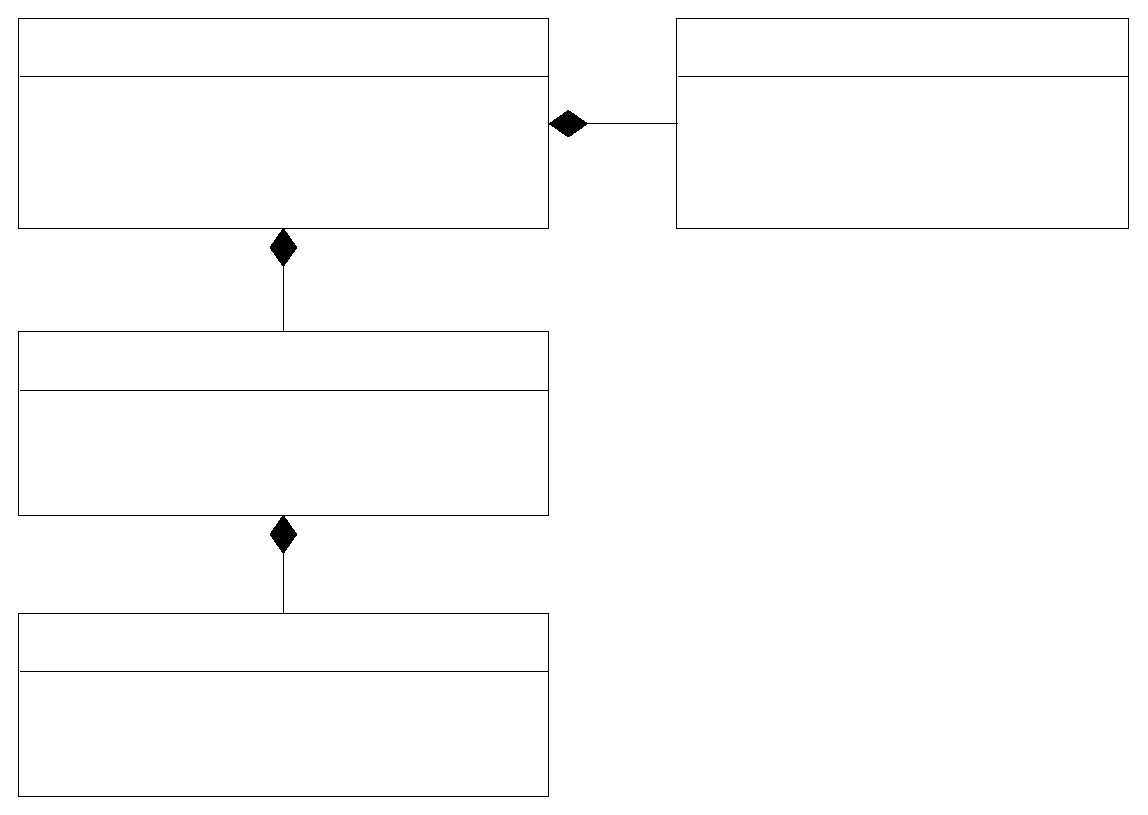
\includegraphics{figs/reference_schema.ssd.fig.eps}%
\end{picture}%
\setlength{\unitlength}{3947sp}%
%
\begingroup\makeatletter\ifx\SetFigFontNFSS\undefined%
\gdef\SetFigFontNFSS#1#2#3#4#5{%
  \reset@font\fontsize{#1}{#2pt}%
  \fontfamily{#3}\fontseries{#4}\fontshape{#5}%
  \selectfont}%
\fi\endgroup%
\begin{picture}(8904,6249)(717,-5908)
\put(7801, 37){\makebox(0,0)[b]{\smash{{\SetFigFontNFSS{10}{12.0}{\rmdefault}{\mddefault}{\updefault}Frame Info}}}}
\put(6061,-353){\makebox(0,0)[lb]{\smash{{\SetFigFontNFSS{10}{12.0}{\rmdefault}{\mddefault}{\updefault}TINFS: Frame Start Date/Time}}}}
\put(6061,-579){\makebox(0,0)[lb]{\smash{{\SetFigFontNFSS{10}{12.0}{\rmdefault}{\mddefault}{\updefault}IFRAM: Identifier}}}}
\put(6053,-803){\makebox(0,0)[lb]{\smash{{\SetFigFontNFSS{10}{12.0}{\rmdefault}{\mddefault}{\updefault}End Timestamp}}}}
\put(6061,-1029){\makebox(0,0)[lb]{\smash{{\SetFigFontNFSS{10}{12.0}{\rmdefault}{\mddefault}{\updefault}BBOX: $\ps{F} \in \Bbb{Z}^3$}}}}
\put(6061,-1253){\makebox(0,0)[lb]{\smash{{\SetFigFontNFSS{10}{12.0}{\rmdefault}{\mddefault}{\updefault}IMC-Identifier}}}}
\put(2851, 14){\makebox(0,0)[b]{\smash{{\SetFigFontNFSS{10}{12.0}{\rmdefault}{\mddefault}{\updefault}Geostream Image}}}}
\put(789,-353){\makebox(0,0)[lb]{\smash{{\SetFigFontNFSS{10}{12.0}{\rmdefault}{\mddefault}{\updefault}$\vs{C}_n$: Radiance}}}}
\put(796,-579){\makebox(0,0)[lb]{\smash{{\SetFigFontNFSS{10}{12.0}{\rmdefault}{\mddefault}{\updefault}$\ps{X}_n \in \vs{Z}^3: X(r,c,F)$}}}}
\put(789,-803){\makebox(0,0)[lb]{\smash{{\SetFigFontNFSS{10}{12.0}{\rmdefault}{\mddefault}{\updefault}$r,c,F$ = row,column,IFRAM}}}}
\put(789,-1029){\makebox(0,0)[lb]{\smash{{\SetFigFontNFSS{10}{12.0}{\rmdefault}{\mddefault}{\updefault}srs: spatial reference frame}}}}
\put(789,-1253){\makebox(0,0)[lb]{\smash{{\SetFigFontNFSS{10}{12.0}{\rmdefault}{\mddefault}{\updefault}mat: transformation matrix}}}}
\put(2851,-2469){\makebox(0,0)[b]{\smash{{\SetFigFontNFSS{10}{12.0}{\rmdefault}{\mddefault}{\updefault}Geostream Frame}}}}
\put(789,-2859){\makebox(0,0)[lb]{\smash{{\SetFigFontNFSS{10}{12.0}{\rmdefault}{\mddefault}{\updefault}$\vs{C}_n$: Radiance}}}}
\put(796,-3083){\makebox(0,0)[lb]{\smash{{\SetFigFontNFSS{10}{12.0}{\rmdefault}{\mddefault}{\updefault}$\ps{X}_n \in \vs{Z}^3: X(r,c,F)$}}}}
\put(789,-3309){\makebox(0,0)[lb]{\smash{{\SetFigFontNFSS{10}{12.0}{\rmdefault}{\mddefault}{\updefault}$F$ is constant}}}}
\put(789,-3533){\makebox(0,0)[lb]{\smash{{\SetFigFontNFSS{10}{12.0}{\rmdefault}{\mddefault}{\updefault}mat: transformation matrix}}}}
\put(3061,-1569){\makebox(0,0)[b]{\smash{{\SetFigFontNFSS{10}{12.0}{\rmdefault}{\mddefault}{\updefault}1}}}}
\put(2641,-2093){\makebox(0,0)[b]{\smash{{\SetFigFontNFSS{10}{12.0}{\rmdefault}{\mddefault}{\updefault}1..n}}}}
\put(2851,-4719){\makebox(0,0)[b]{\smash{{\SetFigFontNFSS{10}{12.0}{\rmdefault}{\mddefault}{\updefault}Geostream Row}}}}
\put(789,-5109){\makebox(0,0)[lb]{\smash{{\SetFigFontNFSS{10}{12.0}{\rmdefault}{\mddefault}{\updefault}$\vs{C}_n$: Radiance}}}}
\put(796,-5333){\makebox(0,0)[lb]{\smash{{\SetFigFontNFSS{10}{12.0}{\rmdefault}{\mddefault}{\updefault}$\ps{X}_n \in \vs{Z}^3: X(r,c,F)$}}}}
\put(789,-5559){\makebox(0,0)[lb]{\smash{{\SetFigFontNFSS{10}{12.0}{\rmdefault}{\mddefault}{\updefault}$F,r$ are constant}}}}
\put(789,-5783){\makebox(0,0)[lb]{\smash{{\SetFigFontNFSS{10}{12.0}{\rmdefault}{\mddefault}{\updefault}mat: transformation matrix}}}}
\put(3061,-3863){\makebox(0,0)[b]{\smash{{\SetFigFontNFSS{10}{12.0}{\rmdefault}{\mddefault}{\updefault}1}}}}
\put(2641,-4343){\makebox(0,0)[b]{\smash{{\SetFigFontNFSS{10}{12.0}{\rmdefault}{\mddefault}{\updefault}1..n}}}}
\put(5131,-729){\makebox(0,0)[b]{\smash{{\SetFigFontNFSS{10}{12.0}{\ttdefault}{\mddefault}{\updefault}1}}}}
\put(5701,-436){\makebox(0,0)[b]{\smash{{\SetFigFontNFSS{10}{12.0}{\ttdefault}{\mddefault}{\updefault}1..n}}}}
\end{picture}%
}
    \caption{Reference schema for GOES data}
    \label{fig:reference_schema}
  \end{center}
\end{figure}

\subsection{Induced Operator Modification}
\label{sec:induced-mod}

Allowing point sets in a streaming system to have an infinite number
of points can lead to some complications for some image algebra
operators, in particular the induced operations, such as $\im{a}
\gamma \im{b}$.  In image algebra, these induced binary operations are
defined only when $\im{a},\im{b} \in \imType{V}{X}$.  For streaming
data, the point set is not known in advance and a processing system
could not verify the point sets were indeed the same.  The basic
induced image operations are therefore inconvenient for a \ac{DSMS}.
Instead, a modified induced operation is introduced to allow for
greater latitude in query execution.  The idea is to perform an
operation on an image when permitted, in this case when both images
share a point.

To compare with the traditional image algebra formulation, a new
notation is temporarily introduced below.  For two images, $\im{a} \in
\imType{V}{X}, \im{b} \in \imType{V}{Y}$ and a binary operation
$\gamma$ on \vs{V},
\begin{align*}
  \im{a} \gamma_\cap \im{b} &=(\im{a} \gamma_\cap \im{b}) \cap (\ps{X} \cap \ps{Y}) \times \vs{V} \quad\quad\text{ or }\\
  &= \{ (\pt{x},a(\pt{x}) \gamma b(\pt{x})) : \pt{x} \in \ps{X} \cap
  \ps{Y} \}
\end{align*}

Figure~\ref{fig:cap} shows the results of this induced operation on
two images with different point sets.

\begin{figure}[htb]
  \centering
{
  \psset{unit=0.4} 
  \subfigure[$\im{a}, \im{b}$]{
    \begin{FramePic}[10,10]
      \roi[style=frame](1,1)(7,7){\im{a}}
      \roi[style=frame](2,2)(9,9){\im{b}}
    \end{FramePic}
  }
  \quad
  \subfigure[$\im{a} +_\cap \im{b}$]{
    \begin{FramePic}[10,10]
      \roi[style=overlap](2,2)(7,7){}
    \end{FramePic}
  }
}
\caption[Induced operation redefinition]{
  Induced operation redefinition.  $\im{a}+\im{b}$ is not defined,
  where $\im{a} +_\cap \im{b}$ is shown}
\label{fig:cap}
\end{figure}

An important feature of this operation that will be used when
optimizing queries is that restrictions can be distributed across
this form of induced operation.  The original induced operation
disallows distributive rules in relation to restrictions. For example,
$\im{a}|_\ps{A} + \im{b}|_\ps{A} \ne (\im{a}+\im{b})|_\ps{A}$ since
the left hand side holds for $\im{a} \in \imType{V}{X}, \im{b} \in
\imType{V}{Y}$ while the right side generally does not.  The redefined
operation $\im{a} +_\cap \im{b}$, however, does allow restrictions to
be distributed.  

In formulations below, the modified intersection operation
will be the default induced operation on images used in the system.
These operator definitions also have the nice property that arbitrary
\vs{V}-valued images can be combined.  Query operator rewrite rules,
further described in Section~\ref{sec:rewrites}, will take advantage
of this formulation.

It is ordering of the geographic point sets that allows images to
be combined in induced operations or other operations.  Because point
sets are ordered, operations are able to determine whether a point
belongs in the union of two point sets by investigating the current
point in the streams.  As some new point from an image stream, \im{a},
arrives in one stream, any points in another stream ordered before
this point can be removed as not belonging to the union of the point
sets, as that point is guaranteed not to be in stream \im{a}.

Neither image restrictions nor extensions are affected by the
indeterminate nature of streaming point sets.  Though the entire point
set for an image may not be known, since image arrives in an order,
enough local information can be used to determine whether points in an
image are involved in restriction and extension operations.  As will
be seen in Chapter~\ref{cha:operators}, compositions or spatial
transforms might require that more than the current point in an image
stream needs to be cached to complete these operations, but they do not
require knowledge of the entire point set and are therefore also
usable without modification.

\section{Query Model}
\label{sec:qm}

Queries in the \ac{GS} system will be based on a particular image
algebra expression.  An individual query will follow an image algebra
template with various parameters specified for the query.

The specific query declaration uses a formulation inspired by \ac{WMS}
specification.  Users specify a specific data product, coordinate
system, spatial \ac{ROI}, temporal extents, and pixel size.  The
\ac{WMS} queries have equivalent image algebra formulations which
are shown for the reference queries.

Query optimization will be discussed in detail in
Chapter~\ref{cha:query}, but an important aspect of optimization is
taking advantage of rules for rewriting a given expression to an
equivalent form.  Some algebraic properties of image algebra are
discussed in Section~\ref{sec:rewrites}.  Image restrictions are once
again a focus of Section~\ref{sec:restriction-types} in combination
with extensions, where a number of potential image results from
queries are discussed and formulated.

\subsection{Reference Queries}
\label{sec:queries2}

With a data model in place, queries are represented as simple
expressions.  Table~\ref{tab:queries} revisits the example queries of
Section~\ref{sec:queries} (page \pageref{sec:queries}) and writes
those queries as image algebra expressions.  As can be seen, the
expressions for these simple queries are quite compact.
%
\begin{table}[hptb]
  \caption{Reference \ac{GOES} queries}
  \centering
  \begin{tabular}{>{}c|l|>{\PBS\raggedright\hspace{0pt}}p{8cm}}

    {\bf Q} & {\bf Image Algebra } & \multicolumn{1}{c}{\bf Description} \\

    \hline
    \hline

    \qry{A} & $\im{C1}|_{\ps{MX}}$ & Query A represents a user requesting Channel 1, (visible) data over a \ac{ROI} covering Mexico.  There are no time constraints on the query.  The resolution corresponds to the default \ac{GOES} data, as does the requested projection \\

    \hline

    \qry{B} & $\im{C1} \oplus \ps{N_{4 \times 4}} \circ LL |_{\ps{NA}}$ & Query B is another query on the visible channel, however in this instance, the user wants the data at a coarser resolution, and projected to a longitude-latitude, (equidistant cylindrical) grid. \\

    \hline

    \qry{C} & $\frac{\im{C2}\oplus \ps{N_{4 \times 4}}-\im{C1}\oplus \ps{N_{4 \times 4}}}{\im{C1}\oplus \ps{N_{4 \times 4}}+\im{C2}\oplus \ps{N_{4 \times 4}}} |_{\ps{NA}} $ & This query represents a user requesting a product, in 
    this case NDVI, which is a normalized difference index using two input channels.  This query is limited to North America. \\

    \hline

    \qry{D} & $\frac{\im{C2}\oplus \ps{N_{8 \times 8}}-\im{C1}\oplus \ps{N_{8 \times 8}}}{\im{C1}\oplus \ps{N_{8 \times 8}}+\im{C2}\oplus \ps{N_{8 \times 8}}} \circ LL |_{\ps{HEMI}} $ & This query represents an NDVI request at a coarse scale and covering the entire northern hemisphere. The requested image is also projected to longitude-latitude. \\

    \hline    
    \qry{E} & $\im{C1}|_{\ps{NA}}|_{\ps{@t}} $ & This query requests visible GOES data, but only the image that occurs at some time, \pt{t}, everyday. \\

    \hline

    \qry{F} & $\im{C1} \circ UTM |_{\ps{CA}}|_{\ps{<\pt{d}}} $ &  This is similar to the query \qry{E}, but also specifies an ending date, \pt{d}, when the query will end. \\

    \hline

    \qry{G} & $\im{C1}|_{\pt{G}}$ & This query asks for image data at a single point.\\

    \hline

    \qry{H} & $\im{C1}\|_{C1(x) > v}$ &  Channel 1, but only in the image where the \emph{pixel values} are greater than some amount $v$. \\ 

  \end{tabular}
  \label{tab:queries}
\end{table}

Most of the queries follow a particular format, being a combination of
induced operations, a neighborhood operation, a restriction, and
finally a spatial transform.  The examples above use a rather loose
notation in defining the parameters of each query, the restriction
\acp{ROI}, and the different spatial transforms used.  One problem
with the current image algebra formulation is there is not a simple
standard method to represent these aspects of the queries.  The
\ac{WMS} specification is used to complete these query specifications,
with a method of describing these parameters.

\subsection{WMS Queries}
\label{sec:wms-queries}

The goal of the \ac{GS} system is to provide users a convenient
interface to \ac{RSI} data, including an easy to use query interface.
Currently, the most common network application interface to general
purpose \ac{GIS} data is through the \ac{OGC}
\acf{WMS}~\cite{openg04web-map}.  The \ac{GS} project adapts the
\ac{WMS} specification as a query specification.  The \ac{WMS}
implementation specification provides an interface to support the
creation and display of registered views of information that come
simultaneously from multiple remote sources.  The implementation
allows a client to access maps from any \ac{WMS} server.  Clients can
also interrogate servers to determine what types of data products are
available from the server.  The \ac{WMS} defines a method to convey
information about what types of \ac{RSI} a service can provide and a
method to convey a request for a particular \ac{RSI} data product.
\ac{WMS} queries are simple URL requests. An example
query looks like the following:
\begin{verbatim}
  http://geostreams.org/wms?VERSION=1.3.0&REQUEST=GetMap
    &LAYERS=NDVI&CRS=epsg:4326&BBOX=-125,19,-65,49&WIDTH=5000&HEIGHT=5000
\end{verbatim}

A selected set of the \ac{WMS} parameters are described in
Table~\ref{tab:wms-getmap-parameters}.  The key parameters are:
\texttt{LAYERS}, which specifies the desired product; \texttt{CRS},
which specifies the output coordinate reference system; \texttt{BBOX},
which specifies the bounding box of the query; and \texttt{WIDTH} and
\texttt{HEIGHT}, which combined, specify the resolution of the image.
\texttt{FORMAT} is a comma limited set of graphic file identifiers,
for example, GeoTIFF.  Currently, no common existing format supports a
geostream image as output.
%
\begin{table}[htb]
  \centering
  \caption{Selected \ac{WMS} \emph{GetMap} parameters}
  \begin{tabular}{c|l}
    Parameter & Description \\
    \hline \hline
%    VERSION=1.3.0 & Request version. \\
%    REQUEST=GetMap & Request name. \\
    LAYERS=layer & one or more map layers.\\
%    STYLES=style & rendering style per requested layer. \\
    CRS=namespace:identifier & Coordinate reference system. \\
    BBOX=minx,miny,maxx,maxy & Bounding box corners in CRS units.\\
    WIDTH=$c$ & Width is $c$ pixels.\\
    HEIGHT=$r$ & Height is $r$ pixels.\\
    FORMAT=output\_format & Output format of map. (STRING)\\
    TRANSPARENT & Background transparency of map. (TRUE or FALSE) \\
    BGCOLOR=HEX & Hexadecimal color for the background. \\
    TIME=time & Time value of layer desired. \\
  \end{tabular}
  \label{tab:wms-getmap-parameters}
\end{table}

The service description component of the \ac{WMS} interface is the
\emph{GetCapabilities} command.  A client issues a
\emph{GetCapabilities} request to the server, and the server responds
with a description of the service.  The description includes what
layers are available from the service and their spatial extents, what
particular spatial reference systems are available, what output
formats, and a number of other parameters.  Using the \ac{WMS}
implementation allows the server to limit the types of queries that
are allowed by users of the system.

By limiting the requests to a finite number of specific products the
server is able to limit the types of induced operations that the user
can specify.  Using the \ac{WMS} implementation the user is only able
to specify particular layers defined by the system.  The server builds
a limited subset of allowed induced operations by creating specialized
layers that encompass these operations.

In a similar manner, the available formats and coordinate reference
systems can also be specified as a limited set of choices to the user.
The capabilities of a server can be thought of as a template on the
allowed queries to the system.  Figure~\ref{fig:wms-queries} shows
such a template designed with the reference queries from
Table~\ref{tab:ref-queries} (page~\pageref{tab:ref-queries}).  Here,
six different layers, including all image channels and the \ac{NDVI}
formula are allowed.  Also allowed are three coordinate system
transformations; the original \ac{GOES} projection $\circ G$, various
\ac{UTM} zones, $\circ UTM$, and longitude latitude, $\circ LL$.

\begin{figure}[htb]
  \centering
  http://$\ldots$LAYERS=$\left\{\begin{array}{c}C1\\C2\\C3\\C4\\C5\\NDVI\end{array}\right\}$\&CRS=$\left\{\begin{array}{c}LL\\UTM\\GOES\end{array}\right\}$\\
  \vspace*{6pt}
  \&WIDTH=\emph{any}\&HEIGHT=\emph{any}\&BBOX=\emph{S,E,W,N}
  \caption{\ac{WMS} queries}
  \label{fig:wms-queries}
\end{figure}


This simple interface does not allow for a sophisticated set of user
queries, but it does investigate the most basic requirements of
serving many spatial restrictions and geometric transformations to
many clients.  The interface allows users to specify specific data
products, coordinate systems, and spatial extents.  Temporal
restrictions can also be identified.  Queries like the reference
queries in Section~\ref{sec:queries} can be specified, as long as the
values of the resultant query are identified as a product in the
server.  The \ac{WMS} specification further simplifies query
formulation by standardizing and simplifying both spatial transforms
and restrictions to a limited but well-defined subset.  In general,
the \ac{WMS} specification limits queries to the form, $\im{a}
\oplus N \circ f |_{X}$, where $\im{a}$, $N$, $f$, and $X$ are
specified in a simple standard way.

\subsection{Rewrite Rules for Image Expressions}
\label{sec:rewrites}

An important part of the query model is that it lends itself to
optimization techniques by the system.  When optimizing a query, it is
necessary to rewrite some expressions into equivalent forms that may
improve performance.  In this section some of the most important
rules involved in rewriting expressions will be discussed.

% One functional rule shows that a series of compositions is simply a
% composition over a new function.  Section~\ref{sec:image-algebra}
% defined the composition operator,
% $\im{a}\circ f \equiv \{(\pt{y},a(f(\pt{y})) : \pt{y}\in\ps{Y}\}$
% where $f:\ps{Y}\to\ps{X}$.  The formulation of two compositions is:
% \[\im{a}\circ f\circ g\equiv \{(\pt{y},a(f(\pt{y})) : \pt{y}\in \ps{Y}\}\circ g \equiv \{(\pt{y},a(f(g(\pt{z}))) : \pt{z}\in\ps{Z}\}\] where
% $f:\ps{Y}\to\ps{Z}$ and $g:\ps{Z}\to\ps{X}$.  The final result is
% still dependent only on the original image \im{a} and the can be
% replaced with a single composition $\im{a}\circ f$ where
% $f(g(z)):\ps{Z}\to\ps{X} \equiv f\circ g$.  This can be used to combine
% multiple composition operations into a single step without the need to
% create intermediate images.

There are a number of rules regarding the restriction operation.
First, a number of identity relations on images are defined:
\begin{align*}
  \im{a} &\equiv \im{a}|_{domain(\im{a})}  \\
  \im{a} &\equiv \im{a}\|_{range(\im{a})} \\
  \im{a} &\equiv \im{a}|^{\im{a}}
\end{align*}

These identity relations simply show that there are obvious
restrictions that do not change an image.  In particular, the
restriction identity $\im{a} = \im{a}|_{domain(\im{a})}$ is useful,
since restrictions have other properties, like the ordering of
multiple restrictions, which prove useful in optimizing queries.
\begin{align*}
\im{a}|_\ps{Y}|_\ps{X}&=(\im{a} \cap (\ps{Y} \times \vs{V}))|_\ps{X} \\
&=(\im{a} \cap (\ps{Y} \times \vs{V})) \cap (\ps{X} \times \vs{V}) \\
&=(\im{a} \cap (\ps{Y}\cap\ps{X}) \times \vs{V}) \\
&=\im{a}_{\ps{X}\cap\ps{Y}} \quad \text{or} \\
&=\im{a}|_\ps{X}|_\ps{Y}
\end{align*}

One result of the above properties is that other restriction
operations can safely be placed in expressions if their point sets are
inclusive of the other restrictions, that is
$\im{a}|_\ps{Y}|_\ps{X}=\im{a}|_\ps{X}$ if $\ps{X}\subset \ps{Y}$.  It
also implies that restrictions can be added into expressions and
distributed through other operations as seen next.

The restriction operation is associative and right distributive over
induced operations with the induced function definition introduced in
Section~\ref{sec:induced-mod}.  For images $\im{a} \in \imType{V}{X}$
and $\im{b} \in \imType{V}{Y}$, using the previously defined rules on
restrictions, this can be shown.
\begin{align*}
  (\im{a} \gamma_\cap \im{b})|_\ps{Z} &=((\im{a} \gamma_\cap \im{b}) \cap (\ps{X} \cap \ps{Y}) \times \vs{V}) \cap \ps{Z} \times \vs{V} \\
  &=((\im{a} \gamma_\cap \im{b}) \cap (\ps{Z} \cap \ps{X} \cap \ps{Y}) \times \vs{V}) \\
  &=\im{a}|_{\ps{X}\cap\ps{Z}} \gamma_\cap \im{b}|_{\ps{Y}\cap\ps{Z}} \\
  &=(\im{a}|_\ps{Z} \gamma_\cap \im{b}|_\ps{Z})
\end{align*}

Spatial transformations also have an identity function with respect to
a restriction.  For an image, $\im{a} \in \imType{V}{X}$, and function
$f: \ps{Y} \rightarrow \ps{X}$, \[ \im{a} \circ f = \im{a}|_{range(f)} \circ f\]

This simply says that a restriction on \im{a} over the range of the
function $f$ does not affect the results of the composition, since
those are the only pixels used in the composition.  This is shown
pictorially in Figure~\ref{fig:rangef}.

\begin{figure}[htb]
  \centering
  \scalebox{0.8}{\begin{picture}(0,0)%
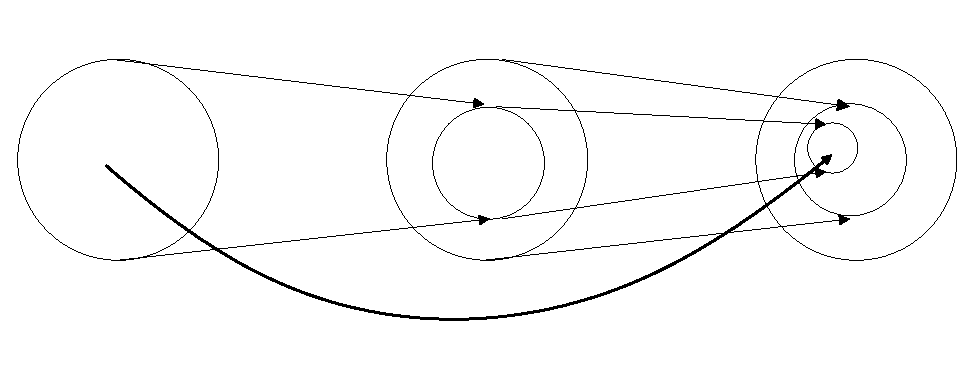
\includegraphics{figs/rangef.fig.eps}%
\end{picture}%
\setlength{\unitlength}{4144sp}%
%
\begingroup\makeatletter\ifx\SetFigFontNFSS\undefined%
\gdef\SetFigFontNFSS#1#2#3#4#5{%
  \reset@font\fontsize{#1}{#2pt}%
  \fontfamily{#3}\fontseries{#4}\fontshape{#5}%
  \selectfont}%
\fi\endgroup%
\begin{picture}(7173,2640)(37,-1799)
\put(631,682){\makebox(0,0)[lb]{\smash{{\SetFigFontNFSS{12}{14.4}{\familydefault}{\mddefault}{\updefault}{\color[rgb]{0,0,0}\ps{Y}}%
}}}}
\put(3398,682){\makebox(0,0)[lb]{\smash{{\SetFigFontNFSS{12}{14.4}{\familydefault}{\mddefault}{\updefault}{\color[rgb]{0,0,0}\ps{X}}%
}}}}
\put(6166,682){\makebox(0,0)[lb]{\smash{{\SetFigFontNFSS{12}{14.4}{\familydefault}{\mddefault}{\updefault}{\color[rgb]{0,0,0}\vs{V}}%
}}}}
\put(2206,-646){\makebox(0,0)[lb]{\smash{{\SetFigFontNFSS{12}{14.4}{\familydefault}{\mddefault}{\updefault}{\color[rgb]{0,0,0}$f$}%
}}}}
\put(4861,434){\makebox(0,0)[lb]{\smash{{\SetFigFontNFSS{12}{14.4}{\familydefault}{\mddefault}{\updefault}{\color[rgb]{0,0,0}\im{a}}%
}}}}
\put(2881,-1726){\makebox(0,0)[lb]{\smash{{\SetFigFontNFSS{12}{14.4}{\familydefault}{\mddefault}{\updefault}{\color[rgb]{0,0,0}$\im{a} \circ f$}%
}}}}
\put(3241,-286){\makebox(0,0)[lb]{\smash{{\SetFigFontNFSS{12}{14.4}{\familydefault}{\mddefault}{\updefault}{\color[rgb]{0,0,0}$range(f)$}%
}}}}
\end{picture}%
}
  \caption{Diagram showing $\im{a} \circ f = \im{a}|_{range(f)} \circ f$}
  \label{fig:rangef}
\end{figure}

Restrictions are not left distributive over spatial transforms.  But
transforms of the point set can be distributed over a composition.
For an image, $\im{a} \in \imType{V}{X}$, and $f: \ps{Y} \rightarrow
\ps{X}$, if $\ps{W} \subseteq \ps{Y}$, then
\begin{align*}
  (\im{a} \circ f)|_{\ps{W}} &= \im{a} \circ (f|_\ps{W}) \\ 
%  &= \im{a}|_{range(f|_{\ps{W}})} \circ (f|_\ps{W}) \\
  &= (\im{a}|_{range(f|_{\ps{W}})} \circ f)|_\ps{W}
\end{align*}
%
Figure~\ref{fig:rangefw} shows this is very similar to the previous
result.

\begin{figure}[htb]
  \centering
  \scalebox{0.8}{\begin{picture}(0,0)%
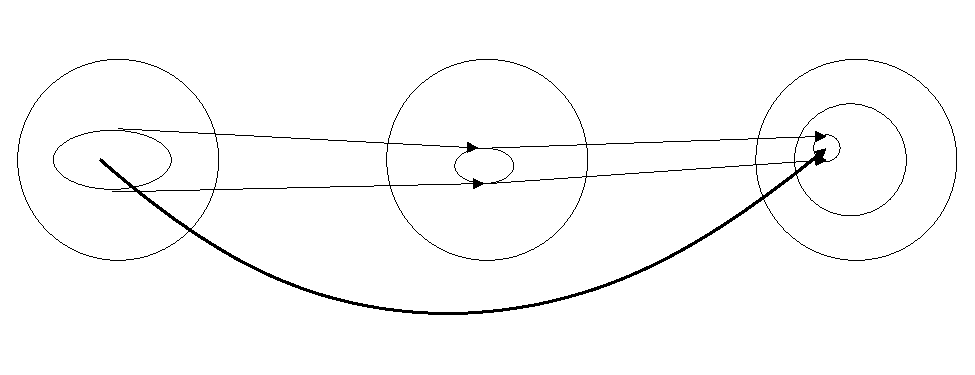
\includegraphics{figs/rangefw.fig.eps}%
\end{picture}%
\setlength{\unitlength}{4144sp}%
%
\begingroup\makeatletter\ifx\SetFigFontNFSS\undefined%
\gdef\SetFigFontNFSS#1#2#3#4#5{%
  \reset@font\fontsize{#1}{#2pt}%
  \fontfamily{#3}\fontseries{#4}\fontshape{#5}%
  \selectfont}%
\fi\endgroup%
\begin{picture}(7173,2595)(37,-1754)
\put(631,682){\makebox(0,0)[lb]{\smash{{\SetFigFontNFSS{12}{14.4}{\familydefault}{\mddefault}{\updefault}{\color[rgb]{0,0,0}\ps{Y}}%
}}}}
\put(3398,682){\makebox(0,0)[lb]{\smash{{\SetFigFontNFSS{12}{14.4}{\familydefault}{\mddefault}{\updefault}{\color[rgb]{0,0,0}\ps{X}}%
}}}}
\put(6166,682){\makebox(0,0)[lb]{\smash{{\SetFigFontNFSS{12}{14.4}{\familydefault}{\mddefault}{\updefault}{\color[rgb]{0,0,0}\vs{V}}%
}}}}
\put(406, 74){\makebox(0,0)[lb]{\smash{{\SetFigFontNFSS{12}{14.4}{\familydefault}{\mddefault}{\updefault}{\color[rgb]{0,0,0}\ps{Y}}%
}}}}
\put(2341,-1681){\makebox(0,0)[lb]{\smash{{\SetFigFontNFSS{12}{14.4}{\familydefault}{\mddefault}{\updefault}{\color[rgb]{0,0,0}$(\im{a} \circ f)|_{\ps{W}}$}%
}}}}
\put(1756,-646){\makebox(0,0)[lb]{\smash{{\SetFigFontNFSS{12}{14.4}{\familydefault}{\mddefault}{\updefault}{\color[rgb]{0,0,0}$f|_{\ps{W}}$}%
}}}}
\put(3016,-16){\makebox(0,0)[lb]{\smash{{\SetFigFontNFSS{12}{14.4}{\familydefault}{\mddefault}{\updefault}{\color[rgb]{0,0,0}$range(f|_{\ps{W}})$}%
}}}}
\end{picture}%
}
  \caption{Diagram showing $(\im{a} \circ f)|_{\ps{W}} = (\im{a}|_{range(\ps{W})} \circ f)|_\ps{W}$}
  \label{fig:rangefw}
\end{figure}

The combination of a neighborhood operation with a restriction is
similar to the above combination of restriction and composition.  The
difference being that a point set $\ps{Z} \subseteq \ps{X}$ needs to
include all points used in the creation of each of the aggregation
points in the restriction on $\ps{W} \subseteq \ps{Y}$, where, as
before, \im{n} is an image where values of \im{n} are point sets,
$n(\pt{y}) \subseteq \ps{X}$.
\begin{align*}
  (\im{a} \oplus \im{n})|_{\ps{W}} &= \{(\pt{y},\sum_{i \in n(\pt{y})} a(\pt{i})) : \pt{y}\in\ps{Y}\} |_\ps{W} \} \\
  &= \{(\pt{y},\sum_{i \in n(\pt{y})} a(\pt{i})) : \pt{y}\in (\ps{Y}\cap\ps{W}) \}
\end{align*}
 
Note that the only values used in \im{a}, are those included in the
summatations from values of $\im{n}|_{\ps{W}}$.  These points can be
collected in a new pointset $\ps{Z}=\bigcap \{ x : x \in n(\pt{y}),
\pt{y} \in \ps{W}\}$. Then, as also shown in Figure~\ref{fig:neighbor-restrict},
\[(\im{a} \oplus \im{n})|_{\ps{W}} = (\im{a}|_{\ps{Z}} \oplus
\im{n})|_{\ps{W}}\]

\begin{figure}[htb]
  \centering
  \scalebox{0.8}{\begin{picture}(0,0)%
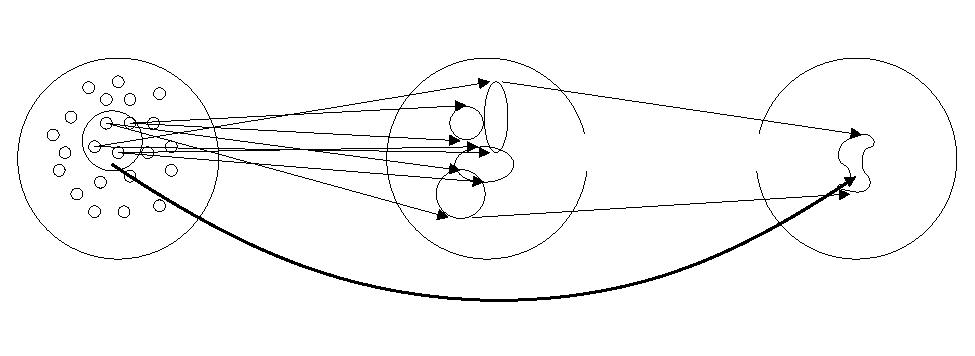
\includegraphics{figs/neighbor-restrict.fig.eps}%
\end{picture}%
\setlength{\unitlength}{4144sp}%
%
\begingroup\makeatletter\ifx\SetFigFontNFSS\undefined%
\gdef\SetFigFontNFSS#1#2#3#4#5{%
  \reset@font\fontsize{#1}{#2pt}%
  \fontfamily{#3}\fontseries{#4}\fontshape{#5}%
  \selectfont}%
\fi\endgroup%
\begin{picture}(7173,2460)(37,-1619)
\put(631,682){\makebox(0,0)[lb]{\smash{{\SetFigFontNFSS{12}{14.4}{\familydefault}{\mddefault}{\updefault}{\color[rgb]{0,0,0}\ps{Y}}%
}}}}
\put(3398,682){\makebox(0,0)[lb]{\smash{{\SetFigFontNFSS{12}{14.4}{\familydefault}{\mddefault}{\updefault}{\color[rgb]{0,0,0}\ps{X}}%
}}}}
\put(6166,682){\makebox(0,0)[lb]{\smash{{\SetFigFontNFSS{12}{14.4}{\familydefault}{\mddefault}{\updefault}{\color[rgb]{0,0,0}\vs{V}}%
}}}}
\put(1756,-646){\makebox(0,0)[lb]{\smash{{\SetFigFontNFSS{12}{14.4}{\familydefault}{\mddefault}{\updefault}{\color[rgb]{0,0,0}\im{n}}%
}}}}
\put(4771,299){\makebox(0,0)[lb]{\smash{{\SetFigFontNFSS{12}{14.4}{\familydefault}{\mddefault}{\updefault}{\color[rgb]{0,0,0}\im{a}}%
}}}}
\put(2341,-1546){\makebox(0,0)[lb]{\smash{{\SetFigFontNFSS{12}{14.4}{\familydefault}{\mddefault}{\updefault}{\color[rgb]{0,0,0}$(\im{a} \oplus \im{n})|_{\ps{W}}$}%
}}}}
\put(3871,-241){\makebox(0,0)[lb]{\smash{{\SetFigFontNFSS{12}{14.4}{\familydefault}{\mddefault}{\updefault}{\color[rgb]{0,0,0}$\bigcap \{ x : x \in n(\pt(w)), \pt{w} \in \ps{W}\}$}%
}}}}
\end{picture}%
}
  \caption[Diagram showing $(\im{a} \oplus \im{n})|_{\ps{W}} = (\im{a}|_{\ps{Z}} \oplus \im{n})|_{\ps{W}}$]{Diagram showing $(\im{a} \oplus \im{n})|_{\ps{W}} = (\im{a}|_{\ps{Z}} \oplus \im{n})|_{\ps{W}}$ where $\ps{Z}=\bigcap \{ x : x \in n(\pt{y}),\pt{y} \in \ps{W}\}$}
  \label{fig:neighbor-restrict}
\end{figure}
 
These rewriting rules will be used in Chapter~\ref{cha:query}, where
cost models are introduced to estimate the benefits of certain query
rewriting strategies.

\subsection{Query Restriction Types}
\label{sec:restriction-types}

One problem that remains with the query model has to do with how to
fill in missing points in a query when not all points exist in the
image stream.  For example, consider three individual image frames
that are being restricted by a query.  The three frames are shown in
Figure~\ref{fig:restriction} labeled \ps{q}, \ps{r}, and \ps{s}.  The
\ac{ROI} for the query is labeled \ps{Q}.
Figure~\ref{fig:restriction} shows the restriction that has been
discussed above.  This returns pixels with points that are in both the
query point set and the image point set.  This means that the result
point set for the query can change from frame to frame.

\begin{figure}[htb]
  \centering
  {
    \psset{unit=0.25}
    \subfigure[Input]{
      \begin{FramePic}[10,10]
        \roi[style=query](5,5)(8,8){\ps{Q}}
        \roi[style=frame](1,1)(9,9){\ps{q}}
        \roi[style=frame](2,2)(7,7){\ps{r}}
        \roi[style=frame](3,3)(9,4){\ps{s}}
      \end{FramePic}
    }
    \subfigure[$q|_Q$]{
      \begin{FramePic}[10,10]
        \roi[style=overlap](5,5)(8,8){}
      \end{FramePic}
    }    
    \subfigure[$r|_Q$]{
      \begin{FramePic}[10,10]
        \roi[style=overlap](5,5)(7,7){}
      \end{FramePic}  
    }
    \subfigure[$s|_Q$]{
      \begin{FramePic}[10,10]
      \end{FramePic}
    }
  }
  \caption{Example image restriction}
  \label{fig:restriction}
\end{figure} 

There are other potential ways to interpret the \ac{WMS} parametrized
query.  For example, the system could return results only from frames
that completely contain the query \ac{ROI}.  Figure~\ref{fig:subset}
shows this example by including a test verifing all points in the
query pointset are also in the incoming image.  Such a test is not
currently represented by the query model.

\begin{figure}[htb]
  \centering
  {
    \psset{unit=0.25}
    \subfigure[Input]{
      \begin{FramePic}[10,10]
        \roi[style=query](5,5)(8,8){$Q$}
        \roi[style=frame](1,1)(9,9){$q$}
        \roi[style=frame](2,2)(7,7){$r$}
        \roi[style=frame](3,3)(9,4){$s$}
      \end{FramePic}      
    }\quad
    \subfigure[$dom(\im{a}|_\ps{Q})=\ps{Q}$]{
      \begin{FramePic}[10,10]
        \roi[style=overlap](5,5)(8,8){}
      \end{FramePic}
    }
  }
  \caption{Complete image subset}
  \label{fig:subset}
\end{figure}


Figure~\ref{fig:extension2} shows how queries could use an image
extension operation to compel each frame to have a common point set.
In this example, $\im{o}$ is taken as an image that covers all of
$\mathbb{Z}^2$, with a null value for all points.  Unlike the domain
restrictions, the extension of a point set onto $\im{o}$ will always
return an image with point set $\ps{Q}$.  This is an important
modification because images that share a common point set can be
combined to form higher dimensional grids.  For example,
$g|^{\im{o}}_\ps{Q}$ would return a set of images with the same point
set.

\begin{figure}[htb]
  \centering
  {
    \psset{unit=0.25}
    \subfigure[Input]{
      \begin{FramePic}[10,10]
        \roi[style=query](5,5)(8,8){$Q$}
        \roi[style=frame](1,1)(9,9){$q$}
        \roi[style=frame](2,2)(7,7){$r$}
        \roi[style=frame](3,3)(9,4){$s$}
      \end{FramePic}
    }
    \subfigure[$q|_\ps{Q}^\im{}$]{
      \begin{FramePic}[10,10]
        \roi[style=overlap](5,5)(8,8){}
      \end{FramePic}
    }
    \subfigure[$r|_\ps{Q}^\im{o}$]{
      \begin{FramePic}[10,10]
        \roi[fillstyle=solid,fillcolor=lightgray](5,5)(8,8){$Q$}
        \roi[style=overlap](5,5)(7,7){}
      \end{FramePic}  
    }
    \subfigure[$s|_\ps{Q}^\im{o}$]{
      \begin{FramePic}[10,10]
        \roi[fillstyle=solid,fillcolor=lightgray](5,5)(8,8){$Q$}
        \roi[style=overlap](5,5)(5,5){}
      \end{FramePic}
    }
    \caption{Image extension example}
    \label{fig:extension2}
  }
\end{figure} 

It would be perfectly reasonable to assume that the queries
represented by the \ac{WMS} syntax contain an implicit extension
operator.  In fact, the standard contains two parameters
\texttt{BGCOLOR} and \texttt{TRANSPARENT} that can allow the user to
specify an extension to the query expression.  Currently, however, the
simplest, non-extension restrictions are adopted for all queries in
the system.

\section{Related Work}

To provide a transformation, point sets need parameters that allow
translation between the raster and model coordinate systems.  There
have been a number of methods to describe this
transformation~\cite{openg01openg-implem, perciv04earth-imager,
  ritter00geotif-format, warmer04gdal-data}.  There are also reviews
of various scenarios for transformation from image to space coordinate
positions.  The \ac{OGC} abstract specification contains a special
topic on Earth Imagery containing descriptions of geometry
models~\cite{perciv04earth-imager}, which describes image
transformations in more detail.  The \ac{OGC} also publishes a
introduction to image geometry models~\cite{whites04some}.  The
implementation used above follows that of the Geotiff
standard~\cite{ritter00geotif-format} and also closely follows the
representation of the \ac{OGC} \ac{GML}
standard~\cite{cox03geogr-markup, whites01defin-data,
  whites05recom-xml}.

In terms of a query language, besides the \ac{OGC} \ac{WMS}
implementation, there exists a more expansive interface specification,
the \acf{WCS}~\cite{evans05web-cover}.  This specification extends the
\ac{WMS} interface to request other image formats rather than the more
picture oriented \ac{WMS} specification.  The \ac{WCS} offers more
control on the format of the retrieved images, and some more
sophistication in the queries, including more specificity on
multi-band images and requesting explicit interpolation routines.  The
above queries could be formulated equally well with the \ac{WCS}.  One
added bonus being that queries could explicitly define an
interpolation strategy to use for spatial transforms.  In a working
environment the \ac{WCS} is probably a more valuable interface.  The
\ac{WMS} is maintained here primarily because of its simplicity.

Gertz~et~al.~\cite{gertz06data-query} also describe the \ac{GS}
project data and query model with a similar emphasis on its
relationship to image algebra.  G\"uting has introduced the ROSE
algebra, another algebra defined on a point
lattice~\cite{gutin95realm-based} focused more on vector \ac{GIS}
data.  Marathe~\cite{marat02query} describes processing techniques
used on \ac{RSI}.

\chapter{Query Processing}
\label{cha:query}

After having defined an image algebra based data model and query
semantics for the \ac{GS} model, and having defined a core set of
operators for the system, this chapter is concerned with developing
optimization strategies for the creation of a \acf{QEP}.  The overall
objective is to determine an optimal, or at least good global \ac{QEP}
that answers all queries in the \ac{DSMS}.  Both single query
optimizations and multi-query optimizations will be discussed.

Because of the nature of the system, where multiple, perhaps
completely disjoint, query plans are being executed, the efficiency of
the system is dependent both on the strategy of execution and the
order of component execution of that strategy as well.  This is shown
in the difference between the \acf{QEG} and the \ac{QEP}.  These two
terms are defined below:

\emph{A \acf{QEG}, is an acyclic directed graph $QEG = (V,E)$ that
  represents the operations to execute all active queries within the
  \acf{DSMS}.  The nodes, $V$, correspond to individual operators
  within the system, and the edges $E$, correspond to data paths from
  one operator to another.  Operator costs are associated with nodes
  and edges carry the defined point sets and data between operators.}

\emph{A \acf{QEP} is a combination of a \ac{QEG}, plus an ordering on the
  nodes of $V$, which satisfies the partial ordering imposed by a
  topological sort of the \ac{QEG}.  }

Defining efficiency requires a definition of a cost model for the
\ac{QEP}.  Section~\ref{sec:cost} defines a few potential cost
models. A graphical representation of these costs will allow for all
cost models to be visualized.  Understanding the costs of different
optimizations requires some estimates of the costs of individual
operators.  Operator costs are also introduced in this section.
Sometimes the ordering in the \ac{QEP} can affect the total cost of a
\ac{QEG}.  This is the case only when memory constraints are included
when calculating the cost of a particular plan.  One result from the
examination of a number of cost models is that optimizations are often
complementary for a number of models.  A cost model based on execution
time is chosen as a representative optimization model, and used in
subsequent sections.

Section~\ref{sec:single-opt} introduces some optimizations for single
queries.  These optimizations primarily deal with rewriting a query to
be more efficient in its computation.  Within a single query,
optimizations will be concerned with the ordering of the operators.
Just as in relational algebra, the image algebra formulation describes
what output images are formed, but these formulations can be rewritten
to produce multiple paths that perform the operation.
Section~\ref{sec:multi-opt} builds on these optimizations to perform
query optimizations considering all queries in the system.  Where
single query optimization develops operator ordering, multi-query
optimization adds additional savings by sharing results between
queries to develop multi-query \ac{QEG}s.

\section{Cost Models}
\label{sec:cost}

In traditional databases, the usual cost model for query processing
algorithms are based on access to secondary storage, typically
counting the number of pages accessed for a particular query.  In the
case of the \ac{DSMS}, however, processing is assumed to occur in
main memory.  Most in-memory cost models attempt to minimize the total
computation cost associated with a \ac{QEG}, where the computation
cost is usually simplified to a single operation, counting the number
of comparisons in a join, for example.  This is a natural cost model
for a \ac{DSMS} as well, since the interest is in pushing data through
the system fast enough to keep up with the incoming stream.  Rather
than counting a single operation, for images, the computation cost
might be the average computation performed on a pixel.

There are other considerations as well.  Computation cost does not
account for the potential limit on the total memory available to the
system.  Since main memory is limited, if total size of the processing
system gets too large, then memory will need to be swapped to
secondary storage, significantly modifying the costs of executing the
\ac{QEG}.  Therefore, other cost models might consider cost models
that monitor and limit the amount of memory used by the system.

Four potential cost models for evaluating different \acp{QEG} are
described in Table~\ref{tab:cost-models}.  Each cost model has a
potential for validity in the system.  While developing an
implementation of the \ac{GS} \ac{DSMS}, the emphasis will be on
minimizing execution time.  In this chapter, examples will compare
\acp{QEG} using different cost models.  Optimization techniques are
broadly applicable between models, and minimizing costs in any one
model typically lowers the cost of the other formulations.
%
\begin{table}[htb]
  \caption{Cost models}
  \centering
  \begin{tabular}{l|>{\PBS\raggedright\hspace{0pt}}p{10cm}}
    Model & Description \\
    \hline \hline
    \emph{Execution} & Minimize the total \acs{CPU} time of the query \\
    \emph{Creation} & Minimize number of new tuples created, or equivalently the total amount of memory used \\
    \emph{Max-Size} & Minimize the maximum instantaneous memory usage \\
    \emph{Size-Time} & Minimize the memory usage of tuples in the system integrated over the time they are required in the \ac{QEP}.  
  \end{tabular}
  \label{tab:cost-models}
\end{table}

For the multi-query models of Section~\ref{sec:multi-opt}, the
\ac{QEG} alone does not contain enough information to determine the
cost of operations and the ordering defined by \ac{QEP} is also
required.  However, some costs can be calculated from the \ac{QEG}
alone.  For example, the \emph{Execution} cost model can be calculated
with a \ac{DFS} through the \ac{QEG}.  For each node, the cost of the
operation can be calculated using only the input point set, which can
define the size of the incoming data, and the node cost.  Summing all
node costs gives the total execution cost for the \ac{QEG}.  The
\emph{Size-Time} cost is most effected by the ordering of operations
within the \ac{QEG}.  In this section, a specific \ac{QEP} is assumed,
the operator ordering is shown explicitly in the graphical
representation of the query plan.

To develop a complete cost model, costs for the individual operators
need to be defined.  Table~\ref{tab:operator-cost} shows some basic
costs for individual operators.  Again, it is assumed that an image
arrives in row-scan order.  The complexity of the operators are given
in terms of $m$, the number of rows sent to the operator.  Because the
constants, $C$ for processing, and $S$ for size, can vary
significantly and are important in cost models, they should not
be ignored in these formulations, and constants are given as functions
of $n$, the number of pixels per row tuple, and $q$, the numbers of
queries in the system.  $h$ indicates the size of the window in a
neighborhood operation.  Also, $m'$ indicates the number of resultant
rows in the new point set from a transformation. For repeating frames
of data $m'=km$, so this is the same order as $m$, and the extra
notation is given mostly as a hint to the change in point sets.
%
\begin{table}[htb]
  \caption{Operator costs}
  \centering
  \begin{tabular}{l|c|c|c|c}
    Operator & CPU & Size & Selectivity & Create \\
    \hline \hline
    $|_\ps{X}$ & $O(\;C_{|}m\;)$ & $O(\;S\;)$ & $\le m$ & 0 \\ 
    $\im{a}\gamma\im{b}\;)$ & $O(\;C_{\gamma}(n)m\;)$ & $O(\;S\;)$ & $m$ & $m$ \\
    $\circ f$ & $O(\;C_{\circ f}(n)m\;)$ & $O(\;S_{\circ f}(n^2)m'\;)$  & $m$ & $m'$ \\    
    $\oplus N_{h \times h}$ & $O(\;C_{\times}(hn)\;)$ & $O(\;S\;)$ & $m$ & $m/h$ \\
    \hline
    \multicolumn{5}{c}{Multi-query} \\
    \hline \hline
    $|_\ps{X}$ (DCT) & $O(\;\approx C(\lg{q})m\;)$ & $O(\;S_{DCT}(q)\;)$ & $\le mq$ & 0 \\ 
    \hline
    \multicolumn{5}{l}{$h$ : neighborhood window} \\
    \multicolumn{5}{l}{$m$ : incoming rows} \\
    \multicolumn{5}{l}{$m' \propto m$ : new rows} \\
    \multicolumn{5}{l}{$n$ : pixels per row} \\
    \multicolumn{5}{l}{$q$ : numbers of queries}
  \end{tabular}

\label{tab:operator-cost}
\end{table}

The \emph{Cost} column identifies the \ac{CPU} cost of each operation.
\emph{Size} indicates the running size of the operator.  The
\emph{Selectivity} column defines whether the operation has any
selectivity.  An important consideration for image algebra queries is
that all operators with the exception of the spatial restriction
operator require creation of new row tuple data into the data stream.
The cost of creating new row tuples has an additional overhead and
will be modeled explicitly in the cost models.  Operator costs are a
function of implementation, and the costs below are further discussed
in Chapter~\ref{cha:operators}.  Except for the restriction operator,
which can operate on complete rows, each operation requires access at
the individual pixel level, and therefore requires times proportional
to the number of pixels, $n$, in the row tuple.  The operator size for
transformations is constant over many rows, but can be quite large, in
relation to other operator sizes, as much as a single image frame.

The table also contains a multi-query restriction operator.  While the
first restriction operator performs a restriction on a single query,
the multi-query restriction operator simultaneously performs
restrictions on many queries.  Use of this operator is deferred until
Section~\ref{sec:multi-opt}.  As with the other entries in the table,
the values are given without proof.  However, where the cost of the
single operators are fairly self explanatory, the multi-query
restriction is not.  These values are dependent on the implementation,
and Chapter~\ref{cha:dct}, which defines the implementation used for
the \ac{GS} project, describes in detail these costs.

These individual operator costs can be combined together to determine
the overall cost of a query.  In this example and throughout this
paper, serial execution of the operators is assumed.  Although
parallel processing is very viable for image processing, developing
cost models is considerably complicated and obfuscates the image
algebra operator costs.  Figure~\ref{fig:NDVI-1} shows a pictorial
representation of the \ac{QEG} for a simplification of query~\qry{C}
(Tables~\ref{tab:ref-queries}~and~\ref{tab:queries}).  These figures
are meant to give a feeling of the \ac{CPU} and memory usage of a
single query in the \ac{GS} system.

The $x$-axis represents time, while the $y$-axis represents memory
usage.  Individual blocks show the lifetime of each row tuple within
the \ac{DSMS}.  The blocks are shown with two shades, the hatched area
represents the cost of creating a new row tuple.  The vertical bars
distinguish the operators that are being executed.  Restriction
operations only direct row tuples and have no data creation costs.

\begin{figure}[htb]
  \centering
  \pstree[treemode=U,nodesep=2pt,levelsep=30pt]{\TR{Q}}{
    \pstree[treemode=U]{\Tb{$|_{NA}$}}{
      \pstree[treemode=U]{\Tcircle{$/$}}{
        \pstree[treemode=U]{\Tcircle{$+$}}{
          \TR[name=C1]{\im{C1}}
          \TR[name=IR]{\im{C2}}
        }
        \Tcircle[name=minus]{$-$}
        \ncline{C1}{minus}
        \ncline{IR}{minus}
      }
    }
  }
  \quad
  \begin{picture}(0,0)%
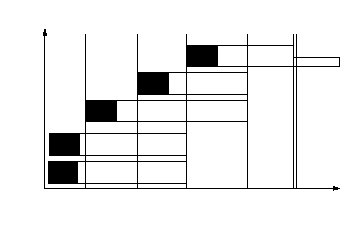
\includegraphics{figs/NDVI-1.fig.eps}%
\end{picture}%
\setlength{\unitlength}{4144sp}%
%
\begingroup\makeatletter\ifx\SetFigFontNFSS\undefined%
\gdef\SetFigFontNFSS#1#2#3#4#5{%
  \reset@font\fontsize{#1}{#2pt}%
  \fontfamily{#3}\fontseries{#4}\fontshape{#5}%
  \selectfont}%
\fi\endgroup%
\begin{picture}(2491,1547)(-14,-642)
\put(1444,746){\makebox(0,0)[lb]{\smash{{\SetFigFontNFSS{5}{6.0}{\familydefault}{\mddefault}{\updefault}{\color[rgb]{0,0,0}$/$}%
}}}}
\put(1048,746){\makebox(0,0)[lb]{\smash{{\SetFigFontNFSS{5}{6.0}{\familydefault}{\mddefault}{\updefault}{\color[rgb]{0,0,0}$-$}%
}}}}
\put(1794,746){\makebox(0,0)[lb]{\smash{{\SetFigFontNFSS{5}{6.0}{\familydefault}{\mddefault}{\updefault}{\color[rgb]{0,0,0}$|_\ps{NA}$}%
}}}}
\put(148,296){\rotatebox{90.0}{\makebox(0,0)[lb]{\smash{{\SetFigFontNFSS{5}{6.0}{\familydefault}{\mddefault}{\updefault}{\color[rgb]{0,0,0}Size}%
}}}}}
\put(  1,-92){\makebox(0,0)[lb]{\smash{{\SetFigFontNFSS{5}{6.0}{\familydefault}{\mddefault}{\updefault}{\color[rgb]{0,0,0}\im{VIS}}%
}}}}
\put(653,746){\makebox(0,0)[lb]{\smash{{\SetFigFontNFSS{5}{6.0}{\familydefault}{\mddefault}{\updefault}{\color[rgb]{0,0,0}$+$}%
}}}}
\put(1325,-627){\makebox(0,0)[lb]{\smash{{\SetFigFontNFSS{5}{6.0}{\familydefault}{\mddefault}{\updefault}{\color[rgb]{0,0,0}Time}%
}}}}
\put(  1,-301){\makebox(0,0)[lb]{\smash{{\SetFigFontNFSS{5}{6.0}{\familydefault}{\mddefault}{\updefault}{\color[rgb]{0,0,0}\im{IR}}%
}}}}
\put(2161,659){\makebox(0,0)[lb]{\smash{{\SetFigFontNFSS{5}{6.0}{\familydefault}{\mddefault}{\updefault}{\color[rgb]{0,0,0}\im{Q}}%
}}}}
\end{picture}%

  \caption[Figure representation of \ac{QEG} for $\frac{\im{C2}-\im{C1}}{\im{C1}+\im{C2}}|_{\ps{NA}}$]{Figure representation of \ac{QEG} for $\frac{\im{C2}-\im{C1}}{\im{C1}+\im{C2}}|_{\ps{NA}}$.  Dark areas identify tuple creation and light areas identify tuple creation.}
  \label{fig:NDVI-1}
\end{figure}

In this figure, the total execution time of the system is equivalent
to the length of the $x$-axis.  The total cost can be expressed as
$3C_{M} + 3nC_{\gamma} + C_{|}$, where $C_{M}$ represents row creation
costs, $C_{\gamma}$ is average cost for per-pixel operations, $n$ is
the number of pixels in the row and $C_{|}$ is the cost for a
restriction.

One cost associated with memory use is to measure the total amount of
new row tuples created which is measured by the $y$-axis as shown in
the figure.  Since every binary operation creates data, the cost of
the operation would be $3C_{M}$.  This cost could also be reasonably
modeled in the previous execution cost model.  Since creation costs
are explicitly included, minimizing tuple creation can use the same
scheme, assigning zero costs to non-creation operations.  This would
be a valid simplification if creation costs dominate.

Two other cost models are apparent.  First, if memory is the limiting
factor, then a \ac{QEG} might aim to limit the total amount of memory
used at any given time.  In the figure, the instantaneous use of
memory is the total height of all bars at any given time.  The maximum
value in this instance is $4C_{M}$, during the second operation.

Finally, a cost model might attempt to limit the total amount of
memory used over the lifetime of the \ac{QEG}.  This is the product of
each memory allocation over its lifetime in the \ac{QEG}.  In
Figure~\ref{fig:NDVI-1}, this corresponds to the sum of the areas of
each bar in the \ac{QEG}.  Adding all bars in this example shows this
cost to be $10 C_{M} + 10nC_{\gamma} + C_{|}$.


\section{Single Query Optimizations}
\label{sec:single-opt}

Evaluating a query using any of the previous cost models depends on
the method used to process the query.  Rewriting a query expression
can result in a more efficient \ac{QEG}. These ideas can be
demonstrated with the previous simplification of Query \qry{C}, with
the image algebra formulation
$\frac{\im{C2}-\im{C1}}{\im{C1}+\im{C2}}|_{\ps{NA}} $.  This can be
realized with a number of different \acp{QEG}, first by using the
distributive property of restrictions over induced operations shown in
Section~\ref{sec:rewrites} (page~\pageref{sec:rewrites}), to move the
restrictions to the input channel streams.

\begin{align*}
\frac{\im{C2}-\im{C1}}{\im{C1}+\im{C2}}|_{\ps{NA}} &= \frac{(\im{C2}-\im{C1})|_{\ps{NA}}}{(\im{C1}+\im{C2})|_{\ps{NA}}} \\
&= \frac{\im{C2}|_{\ps{NA}}-\im{C1}|_{\ps{NA}}}{\im{C1}|_{\ps{NA}}+\im{C2}|_{\ps{NA}}}
\end{align*}

Figures~\ref{fig:NDVI-2}~and~\ref{fig:NDVI-3} show two other
formulations.  One plan simply merges all induced operations
(Figure~\ref{fig:NDVI-2}), the other (Figure~\ref{fig:NDVI-3})
distributes restrictions over the inputs, and merges the induced
operations.  The various costs for the model described in
Section~\ref{sec:cost} are summarized in Table~\ref{tab:ndvi-summary}
for all three formulations.  All variables have been introduced except
for $s$, which is the selectivity of the restriction operator.

\begin{figure}[htb]
  \centering
  \pstree[treemode=U,nodesep=2pt,levelsep=30pt]{\TR{Q}}{
    \pstree[treemode=U]{\Tb{$|_{NA}$}}{    
      \pstree[treemode=U]{\Tcircle{$f()$}}
      {
        \TR[name=C1]{\im{C1}}
        \TR[name=IR]{\im{C2}}
      }
    }
  }
  \quad
  \begin{picture}(0,0)%
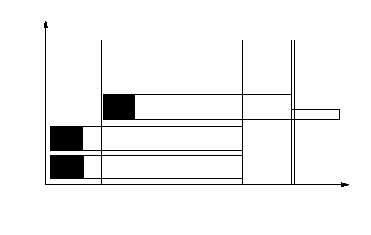
\includegraphics{figs/NDVI-2.fig.eps}%
\end{picture}%
\setlength{\unitlength}{4144sp}%
%
\begingroup\makeatletter\ifx\SetFigFontNFSS\undefined%
\gdef\SetFigFontNFSS#1#2#3#4#5{%
  \reset@font\fontsize{#1}{#2pt}%
  \fontfamily{#3}\fontseries{#4}\fontshape{#5}%
  \selectfont}%
\fi\endgroup%
\begin{picture}(2557,1532)(-14,-681)
\put(153,282){\rotatebox{90.0}{\makebox(0,0)[lb]{\smash{{\SetFigFontNFSS{5}{6.0}{\familydefault}{\mddefault}{\updefault}{\color[rgb]{0,0,0}Size}%
}}}}}
\put(1360,-666){\makebox(0,0)[lb]{\smash{{\SetFigFontNFSS{5}{6.0}{\familydefault}{\mddefault}{\updefault}{\color[rgb]{0,0,0}Time}%
}}}}
\put(  1,-331){\makebox(0,0)[lb]{\smash{{\SetFigFontNFSS{5}{6.0}{\familydefault}{\mddefault}{\updefault}{\color[rgb]{0,0,0}\im{IR}}%
}}}}
\put(  1,-116){\makebox(0,0)[lb]{\smash{{\SetFigFontNFSS{5}{6.0}{\familydefault}{\mddefault}{\updefault}{\color[rgb]{0,0,0}\im{VIS}}%
}}}}
\put(2161,209){\makebox(0,0)[lb]{\smash{{\SetFigFontNFSS{5}{6.0}{\familydefault}{\mddefault}{\updefault}{\color[rgb]{0,0,0}\im{Q}}%
}}}}
\put(811,344){\makebox(0,0)[lb]{\smash{{\SetFigFontNFSS{5}{6.0}{\familydefault}{\mddefault}{\updefault}{\color[rgb]{0,0,0}$f(\im{VIS},\im{IR})$}%
}}}}
\put(1756,344){\makebox(0,0)[lb]{\smash{{\SetFigFontNFSS{5}{6.0}{\familydefault}{\mddefault}{\updefault}{\color[rgb]{0,0,0}$|_\ps{NA}$}%
}}}}
\end{picture}%

  \caption{\ac{QEG} for query \qry{C} with merged algebraic operations}
  \label{fig:NDVI-2}
\end{figure}

\begin{figure}[htb]
  \centering
  \pstree[treemode=U,nodesep=2pt,levelsep=30pt]{\TR{Q}}{
    \pstree[treemode=U]{\Tcircle{$f()$}}
    {
      \pstree[treemode=U]{\Tb{$|_{NA}$}}{\TR[name=C1]{\im{C1}}}
      \pstree[treemode=U]{\Tb{$|_{NA}$}}{\TR[name=C1]{\im{C2}}}
    }
  }
  \quad
  \begin{picture}(0,0)%
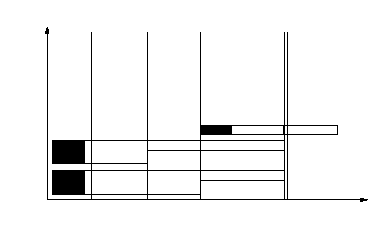
\includegraphics{figs/NDVI-3.fig.eps}%
\end{picture}%
\setlength{\unitlength}{4144sp}%
%
\begingroup\makeatletter\ifx\SetFigFontNFSS\undefined%
\gdef\SetFigFontNFSS#1#2#3#4#5{%
  \reset@font\fontsize{#1}{#2pt}%
  \fontfamily{#3}\fontseries{#4}\fontshape{#5}%
  \selectfont}%
\fi\endgroup%
\begin{picture}(2699,1661)(-14,-764)
\put(161,251){\rotatebox{90.0}{\makebox(0,0)[lb]{\smash{{\SetFigFontNFSS{5}{6.0}{\familydefault}{\mddefault}{\updefault}{\color[rgb]{0,0,0}Size}%
}}}}}
\put(1437,-749){\makebox(0,0)[lb]{\smash{{\SetFigFontNFSS{5}{6.0}{\familydefault}{\mddefault}{\updefault}{\color[rgb]{0,0,0}Time}%
}}}}
\put(  1,-169){\makebox(0,0)[lb]{\smash{{\SetFigFontNFSS{5}{6.0}{\familydefault}{\mddefault}{\updefault}{\color[rgb]{0,0,0}\im{VIS}}%
}}}}
\put(  1,-396){\makebox(0,0)[lb]{\smash{{\SetFigFontNFSS{5}{6.0}{\familydefault}{\mddefault}{\updefault}{\color[rgb]{0,0,0}\im{IR}}%
}}}}
\put(582,738){\makebox(0,0)[lb]{\smash{{\SetFigFontNFSS{5}{6.0}{\familydefault}{\mddefault}{\updefault}{\color[rgb]{0,0,0}$|_\ps{NA}$}%
}}}}
\put(1035,738){\makebox(0,0)[lb]{\smash{{\SetFigFontNFSS{5}{6.0}{\familydefault}{\mddefault}{\updefault}{\color[rgb]{0,0,0}$|_\ps{NA}$}%
}}}}
\put(1490,738){\makebox(0,0)[lb]{\smash{{\SetFigFontNFSS{5}{6.0}{\familydefault}{\mddefault}{\updefault}{\color[rgb]{0,0,0}$f(\im{VIS},\im{IR})$}%
}}}}
\put(2116,119){\makebox(0,0)[lb]{\smash{{\SetFigFontNFSS{5}{6.0}{\familydefault}{\mddefault}{\updefault}{\color[rgb]{0,0,0}\im{Q}}%
}}}}
\end{picture}%

\caption{\ac{QEG} for query \qry{C} with distributed restrictions}
\label{fig:NDVI-3}
\end{figure}
%
\begin{table}[htb]
  \centering
  \caption{Query cost summary for $\frac{\im{C2}-\im{C1}}{\im{C1}+\im{C2}}|_{\ps{NA}} $}
  \begin{tabular}{c|c|c|c|c}
    Plan & Execution & Creation & Max Size & Size-Time \\
    \hline \hline
    Figure~\ref{fig:NDVI-1} & $3 C_{M} + 3 n C_{\gamma} + C_{|}$ & 3 & 4 & $10 C_{M} + 10 n C_{\gamma} + C_{|}$ \\
    Figure~\ref{fig:NDVI-2} & $C_{M} + 3 n C_{\gamma} + C_{|}$ & 1 & 3 & $3 C_{M} + 3 n C_{\gamma} + C_{|}$ \\
    Figure~\ref{fig:NDVI-3} & $s C_{M} + 3 s n C_{\gamma} + 2 C_{|}$ & s & max(2,3s) & $3 s C_{M} + 3 s n C_{\gamma} + (3+s) C_{|}$ 
  \end{tabular}
  \label{tab:ndvi-summary}
\end{table}

Determining each individual cost is fairly simple to do given the
graphical representation of the query plans.  For the Execution cost,
the time, or x-axis, is calculated for the plan.  The costs measured
between each set of bars is based on the operation, which is
identified at the top of the graph.  In addition, the tuple creation
costs, identified by the dark regions in the graphs, also need to be
added in the cost.  The creation costs of the original tuples is not
included in the cost. Using Figure~\ref{fig:NDVI-1} as an example,
there are three new tuples created, $3 C_{M}$.  There are also three
induced operations over $n$ pixels per row, $3 n  C_{\gamma}$, and one
final restriction, $C_{|}$.

The \emph{Creation} cost simply counts the new tuples created.  The
\emph{Max-Size} cost, counts the maximum number of tuples being used
at any one time.  This is a measure of the instantaneous use of
memory.

For the \emph{Size-Time} cost, the time is summed for each row tuple
in the plan.  Again, the costs measured between each set of bars is
based on the operation, which is identified at the top of the graph.
Now all the tuples active in the plan at that time are included in the
cost.

As with the \emph{Execution} cost, tuple creation costs are also
included.  Figure~\ref{fig:NDVI-1} will be used as an example.  The
first time a tuple is created, there are three total tuples in the
system, so that cost is $3 C_{M}$.  The second time, there are four
active tuples, and the final creation has three active tuples.  The
total cost is then $10 C_{M}$.  The number of tuples active for the
induced operators are 3, 4, and 3, so that cost is $10 n C_{\gamma}$.
Finally, there is one active tuple on the final restriction so that
cost is $C_{|}$.  A similar strategy is used for determining the costs
of other plans.  When there is some selectivity involved in an
operation, this limits the number of tuples in subsequent steps, and
affects the costs as well.  For example in Figure~\ref{fig:NDVI-3},
moving the restrictions toward the incoming channels means that only
$s$ tuples make it through the restriction operators and so only $s
C_{M}$ tuples are created.  That also limits the number of rows in the
induced operation step as well, so that has a cost of $3 s n
C_{\gamma}$.  The constant 3 is retained even though there is only one
operation.  In Figure~\ref{fig:NDVI-3}, there are 2 restrictions, so
the total execution time is $s C_{M} + 3 s n C_{\gamma} + 2 C_{|}$.

Some simple optimization techniques present themselves.  First,
merging induced operations is always a good idea for optimizing single
queries, as intermediate row tuple creation steps are not used.  Also,
while the cost of the merged induced operation is considered
equal to the sum of the per-pixel costs all operations, it is more of an
upper bound on this cost, since merging operations also limits the
number of pixel accesses that take place.

Other optimizations depend on the individual operator costs.  If row
allocations and restrictions are not expensive, that is $C_{M} \approx
C_{\gamma} \approx C_{|}$, then for row tuples with $n>>1$, the cost
model simplifies to counting only induced operations.  In this case
distributing restrictions always saves cost.  If instead allocations
are very expensive, i.e., $C_{M} >> C_{\gamma}$, then the cost models reduce
to counting allocations.  Again, distributing restrictions makes
sense.

In fact, the only time that distributing restrictions does not save cost
is if either $C_{|}$ is very high, or if the selectivity on the
restriction is nearly 1, as shown in the comparison of execution time
costs shown below.

\begin{gather*}
C_{M} + 3 n C_{\gamma} + C_{|} <  s C_{M} + 3 s n C_{\gamma} + 2 C_{|} \\
\equiv C_{M} + 3 n C_{\gamma} + C_{|} <  s (C_{M} + 3 n C_{\gamma} ) + 2 C_{|} \\
\equiv 1 - \frac{C_{|}}{C_{M} + 3 n C_{\gamma}}  <  s \\
\equiv 1 - s < \frac{C_{|}}{C_{M} + 3 n C_{\gamma}}
\end{gather*}

This shows that in systems where restriction costs are not high,
distributing restrictions will almost always result in optimal
solutions.  These optimizations are with respect to the execution time
cost model, but examination of Table~\ref{tab:ndvi-summary} shows this
plan is optimal for all plans.  This is mainly because minimizing
tuple creation costs will also limit the amount of memory used by the
query.

\subsection{Memory Management}
\label{sec:memory-management}

Normal memory allocation requests in a program can be very expensive
in relation to other costs, and in designing a \ac{DSMS}, it is
apparent that keeping tuple creation costs low by developing a
specialized memory management system can reduce query costs.  This is
discussed in Section~\ref{sec:on-memory}.  However, other memory costs
could be affected by modifications of the operators themselves.  For
induced operations, rather than output tuples being created, the input
tuples could sometimes be reused to hold the output values.  This
results in savings for most cost models.  Figure~\ref{fig:NDVI-r}
shows \ac{QEG} diagrams utilizing tuple reuse, and
Table~\ref{tab:ndvi-summary-r} summarizes the new costs.

\begin{figure}[htb]
  \centering
  \subfigure[No optimizations]{
     \scalebox{0.82}{\begin{picture}(0,0)%
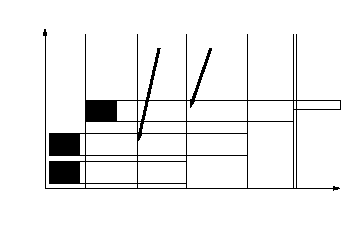
\includegraphics{figs/NDVI-r-1.fig.eps}%
\end{picture}%
\setlength{\unitlength}{4144sp}%
%
\begingroup\makeatletter\ifx\SetFigFontNFSS\undefined%
\gdef\SetFigFontNFSS#1#2#3#4#5{%
  \reset@font\fontsize{#1}{#2pt}%
  \fontfamily{#3}\fontseries{#4}\fontshape{#5}%
  \selectfont}%
\fi\endgroup%
\begin{picture}(2492,1547)(-14,-642)
\put(149,296){\rotatebox{90.0}{\makebox(0,0)[lb]{\smash{{\SetFigFontNFSS{5}{6.0}{\familydefault}{\mddefault}{\updefault}{\color[rgb]{0,0,0}Size}%
}}}}}
\put(1326,-627){\makebox(0,0)[lb]{\smash{{\SetFigFontNFSS{5}{6.0}{\familydefault}{\mddefault}{\updefault}{\color[rgb]{0,0,0}Time}%
}}}}
\put(  1,-92){\makebox(0,0)[lb]{\smash{{\SetFigFontNFSS{5}{6.0}{\familydefault}{\mddefault}{\updefault}{\color[rgb]{0,0,0}\im{VIS}}%
}}}}
\put(  1,-302){\makebox(0,0)[lb]{\smash{{\SetFigFontNFSS{5}{6.0}{\familydefault}{\mddefault}{\updefault}{\color[rgb]{0,0,0}\im{IR}}%
}}}}
\put(1444,746){\makebox(0,0)[lb]{\smash{{\SetFigFontNFSS{5}{6.0}{\familydefault}{\mddefault}{\updefault}{\color[rgb]{0,0,0}$/$}%
}}}}
\put(1049,746){\makebox(0,0)[lb]{\smash{{\SetFigFontNFSS{5}{6.0}{\familydefault}{\mddefault}{\updefault}{\color[rgb]{0,0,0}$-$}%
}}}}
\put(653,746){\makebox(0,0)[lb]{\smash{{\SetFigFontNFSS{5}{6.0}{\familydefault}{\mddefault}{\updefault}{\color[rgb]{0,0,0}$+$}%
}}}}
\put(1794,746){\makebox(0,0)[lb]{\smash{{\SetFigFontNFSS{5}{6.0}{\familydefault}{\mddefault}{\updefault}{\color[rgb]{0,0,0}$|_\ps{NA}$}%
}}}}
\put(2206,344){\makebox(0,0)[lb]{\smash{{\SetFigFontNFSS{5}{6.0}{\familydefault}{\mddefault}{\updefault}{\color[rgb]{0,0,0}\im{Q}}%
}}}}
\end{picture}%
}
  }
  \subfigure[Merge induced operations]{
     \scalebox{0.82}{\begin{picture}(0,0)%
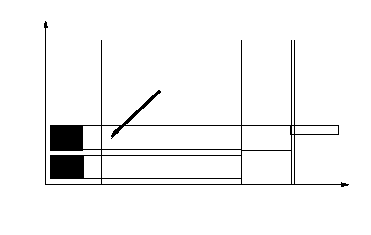
\includegraphics{figs/NDVI-r-2.fig.eps}%
\end{picture}%
\setlength{\unitlength}{4144sp}%
%
\begingroup\makeatletter\ifx\SetFigFontNFSS\undefined%
\gdef\SetFigFontNFSS#1#2#3#4#5{%
  \reset@font\fontsize{#1}{#2pt}%
  \fontfamily{#3}\fontseries{#4}\fontshape{#5}%
  \selectfont}%
\fi\endgroup%
\begin{picture}(2557,1532)(-14,-681)
\put(153,282){\rotatebox{90.0}{\makebox(0,0)[lb]{\smash{{\SetFigFontNFSS{5}{6.0}{\familydefault}{\mddefault}{\updefault}{\color[rgb]{0,0,0}Size}%
}}}}}
\put(1360,-666){\makebox(0,0)[lb]{\smash{{\SetFigFontNFSS{5}{6.0}{\familydefault}{\mddefault}{\updefault}{\color[rgb]{0,0,0}Time}%
}}}}
\put(  1,-116){\makebox(0,0)[lb]{\smash{{\SetFigFontNFSS{5}{6.0}{\familydefault}{\mddefault}{\updefault}{\color[rgb]{0,0,0}\im{VIS}}%
}}}}
\put(  1,-331){\makebox(0,0)[lb]{\smash{{\SetFigFontNFSS{5}{6.0}{\familydefault}{\mddefault}{\updefault}{\color[rgb]{0,0,0}\im{IR}}%
}}}}
\put(789,337){\makebox(0,0)[lb]{\smash{{\SetFigFontNFSS{5}{6.0}{\familydefault}{\mddefault}{\updefault}{\color[rgb]{0,0,0}$f(\im{VIS},\im{IR})$}%
}}}}
\put(1722,337){\makebox(0,0)[lb]{\smash{{\SetFigFontNFSS{5}{6.0}{\familydefault}{\mddefault}{\updefault}{\color[rgb]{0,0,0}$|_\ps{NA}$}%
}}}}
\put(2161, 74){\makebox(0,0)[lb]{\smash{{\SetFigFontNFSS{5}{6.0}{\familydefault}{\mddefault}{\updefault}{\color[rgb]{0,0,0}\im{Q}}%
}}}}
\end{picture}%
}
  }
  \subfigure[Distribute restrictions]{
     \scalebox{0.82}{\begin{picture}(0,0)%
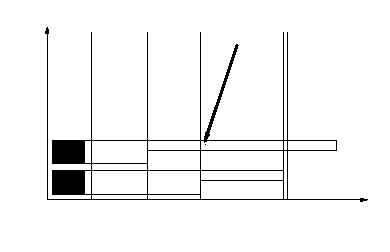
\includegraphics{figs/NDVI-r-3.fig.eps}%
\end{picture}%
\setlength{\unitlength}{4144sp}%
%
\begingroup\makeatletter\ifx\SetFigFontNFSS\undefined%
\gdef\SetFigFontNFSS#1#2#3#4#5{%
  \reset@font\fontsize{#1}{#2pt}%
  \fontfamily{#3}\fontseries{#4}\fontshape{#5}%
  \selectfont}%
\fi\endgroup%
\begin{picture}(2699,1662)(-14,-764)
\put(161,251){\rotatebox{90.0}{\makebox(0,0)[lb]{\smash{{\SetFigFontNFSS{5}{6.0}{\familydefault}{\mddefault}{\updefault}{\color[rgb]{0,0,0}Size}%
}}}}}
\put(1437,-749){\makebox(0,0)[lb]{\smash{{\SetFigFontNFSS{5}{6.0}{\familydefault}{\mddefault}{\updefault}{\color[rgb]{0,0,0}Time}%
}}}}
\put(  1,-170){\makebox(0,0)[lb]{\smash{{\SetFigFontNFSS{5}{6.0}{\familydefault}{\mddefault}{\updefault}{\color[rgb]{0,0,0}\im{VIS}}%
}}}}
\put(  1,-396){\makebox(0,0)[lb]{\smash{{\SetFigFontNFSS{5}{6.0}{\familydefault}{\mddefault}{\updefault}{\color[rgb]{0,0,0}\im{IR}}%
}}}}
\put(582,739){\makebox(0,0)[lb]{\smash{{\SetFigFontNFSS{5}{6.0}{\familydefault}{\mddefault}{\updefault}{\color[rgb]{0,0,0}$|_\ps{NA}$}%
}}}}
\put(1035,739){\makebox(0,0)[lb]{\smash{{\SetFigFontNFSS{5}{6.0}{\familydefault}{\mddefault}{\updefault}{\color[rgb]{0,0,0}$|_\ps{NA}$}%
}}}}
\put(1490,739){\makebox(0,0)[lb]{\smash{{\SetFigFontNFSS{5}{6.0}{\familydefault}{\mddefault}{\updefault}{\color[rgb]{0,0,0}$f(\im{VIS},\im{IR})$}%
}}}}
\put(2116, 29){\makebox(0,0)[lb]{\smash{{\SetFigFontNFSS{5}{6.0}{\familydefault}{\mddefault}{\updefault}{\color[rgb]{0,0,0}\im{Q}}%
}}}}
\end{picture}%
}
  }
  \caption{\acp{QEG} for $\frac{\im{C2}-\im{C1}}{\im{C1}+\im{C2}}|_{\ps{NA}}$ with reuse}
  \label{fig:NDVI-r}
\end{figure}
%
\begin{table}
  \centering

  \caption{Cost summary for query \qry{C} with tuple reuse}
  \begin{tabular}{l|c|c|c|c}
    Plan & Execution & Creation & Max Size & Size-Time \\
    \hline \hline
    Figure~\ref{fig:NDVI-1} & $C_{M} + 3 m C_{\gamma} + C_{|}$ & 1 & 3 & $3 C_{M} + 8 n C_{\gamma} + C_{|}$ \\
    Figure~\ref{fig:NDVI-2} & $3 n C_{\gamma} + C_{|}$ & 0 & 2 & $6 n C_{\gamma} + C_{|}$ \\
    Figure~\ref{fig:NDVI-3} & $3 s n C_{\gamma} + 2 C_{|}$ & 0 & 2s & $2 s n C_{\gamma} + (3+s) C_{|}$ 
  \end{tabular}
  \label{tab:ndvi-summary-r}
\end{table}

Tuple reuse requires more sophisticated execution plans that order
operations such that tuples are only marked for reuse inside
operations when they are no longer needed for other operations.  In
the implementation described in Chapter~\ref{cha:operators}, a memory
management system based on reference counting is used, and the
optimizer does not reuse tuples within operations.  One practical
reason for this, also discussed in Chapter~\ref{cha:operators}, is
that some operations hold input tuples for a short time waiting for
more input.  If these queues are hidden from the optimizer, it can't
be sure of when tuple data can be overwritten.

\subsection{Neighborhood Operations}
\label{sec:nbr-opt}

The complete formulation of query~\qry{C} also contained a
neighborhood operation, $\oplus \ps{N_{4 \times 4}}$.  How
neighborhood operations are included into the single query
optimizations is also an important question.  There is less ability to
rewrite the neighborhood operations within an operation, because they
cannot be distributed across induced operations or spatial transforms.
As an example, it is clear that for some single valued induced
operation, $f$, on image \im{a} with an associated neighborhood
summation, $f(\im{a})\oplus \im{N} \ne f(\im{a}\oplus\im{N})$.
Figure~\ref{fig:neighbor-opt} shows a concrete example of this, using
query~\qry{C}, where the result for a single pixel of data changes
with the ordering of the operations.  Section~\ref{sec:wms-queries},
described the formulation of the queries in the \ac{GS} system.  These
queries included specification of an implicit neighborhood averaging
operation.  For all queries that operation is realized directly on the
input image channels from \ac{GOES}.  Moving neighborhood operations
to the input channels ensures the query results are most consistent
with the incoming \ac{RSI} data.

\begin{figure}[htb]
  \centering
  \scalebox{0.8}{\begin{picture}(0,0)%

\includegraphics{figs/neighbor-math.fig.eps}%
\end{picture}%
\setlength{\unitlength}{4144sp}%
%
\begingroup\makeatletter\ifx\SetFigFontNFSS\undefined%
\gdef\SetFigFontNFSS#1#2#3#4#5{%
  \reset@font\fontsize{#1}{#2pt}%
  \fontfamily{#3}\fontseries{#4}\fontshape{#5}%
  \selectfont}%
\fi\endgroup%
\begin{picture}(6639,3001)(1114,-2555)
\put(1711,119){\makebox(0,0)[lb]{\smash{{\SetFigFontNFSS{14}{16.8}{\familydefault}{\mddefault}{\updefault}{\color[rgb]{0,0,0}5}%
}}}}
\put(1306,-376){\makebox(0,0)[lb]{\smash{{\SetFigFontNFSS{14}{16.8}{\familydefault}{\mddefault}{\updefault}{\color[rgb]{0,0,0}3}%
}}}}
\put(1216,119){\makebox(0,0)[lb]{\smash{{\SetFigFontNFSS{14}{16.8}{\familydefault}{\mddefault}{\updefault}{\color[rgb]{0,0,0}10}%
}}}}
\put(1711,-376){\makebox(0,0)[lb]{\smash{{\SetFigFontNFSS{14}{16.8}{\familydefault}{\mddefault}{\updefault}{\color[rgb]{0,0,0}6}%
}}}}
\put(1711,-1636){\makebox(0,0)[lb]{\smash{{\SetFigFontNFSS{14}{16.8}{\familydefault}{\mddefault}{\updefault}{\color[rgb]{0,0,0}5}%
}}}}
\put(1306,-2131){\makebox(0,0)[lb]{\smash{{\SetFigFontNFSS{14}{16.8}{\familydefault}{\mddefault}{\updefault}{\color[rgb]{0,0,0}3}%
}}}}
\put(1216,-1636){\makebox(0,0)[lb]{\smash{{\SetFigFontNFSS{14}{16.8}{\familydefault}{\mddefault}{\updefault}{\color[rgb]{0,0,0}10}%
}}}}
\put(1711,-2131){\makebox(0,0)[lb]{\smash{{\SetFigFontNFSS{14}{16.8}{\familydefault}{\mddefault}{\updefault}{\color[rgb]{0,0,0}6}%
}}}}
\put(4276,-736){\makebox(0,0)[lb]{\smash{{\SetFigFontNFSS{14}{16.8}{\familydefault}{\mddefault}{\updefault}{\color[rgb]{0,0,0}$N_{2 \times 2}$}%
}}}}
\put(5446,-736){\makebox(0,0)[lb]{\smash{{\SetFigFontNFSS{14}{16.8}{\familydefault}{\mddefault}{\updefault}{\color[rgb]{0,0,0}$N_{2 \times 2}$}%
}}}}
\put(6976,-2491){\makebox(0,0)[lb]{\smash{{\SetFigFontNFSS{14}{16.8}{\familydefault}{\mddefault}{\updefault}{\color[rgb]{0,0,0}$N_{2 \times 2}$}%
}}}}
\put(4636,-2491){\makebox(0,0)[lb]{\smash{{\SetFigFontNFSS{14}{16.8}{\familydefault}{\mddefault}{\updefault}{\color[rgb]{0,0,0}$\frac{C2-C1}{C2+C1}$}%
}}}}
\put(6976,-736){\makebox(0,0)[lb]{\smash{{\SetFigFontNFSS{14}{16.8}{\familydefault}{\mddefault}{\updefault}{\color[rgb]{0,0,0}$\frac{C2-C1}{C2+C1}$}%
}}}}
\put(5446,-106){\makebox(0,0)[lb]{\smash{{\SetFigFontNFSS{14}{16.8}{\familydefault}{\mddefault}{\updefault}{\color[rgb]{0,0,0} 14}%
}}}}
\put(4366,-106){\makebox(0,0)[lb]{\smash{{\SetFigFontNFSS{14}{16.8}{\familydefault}{\mddefault}{\updefault}{\color[rgb]{0,0,0}6}%
}}}}
\put(2828,-781){\makebox(0,0)[lb]{\smash{{\SetFigFontNFSS{14}{16.8}{\familydefault}{\mddefault}{\updefault}{\color[rgb]{0,0,0}C2}%
}}}}
\put(1433,-781){\makebox(0,0)[lb]{\smash{{\SetFigFontNFSS{14}{16.8}{\familydefault}{\mddefault}{\updefault}{\color[rgb]{0,0,0}C1}%
}}}}
\put(1433,-2536){\makebox(0,0)[lb]{\smash{{\SetFigFontNFSS{14}{16.8}{\familydefault}{\mddefault}{\updefault}{\color[rgb]{0,0,0}C1}%
}}}}
\put(2828,-2536){\makebox(0,0)[lb]{\smash{{\SetFigFontNFSS{14}{16.8}{\familydefault}{\mddefault}{\updefault}{\color[rgb]{0,0,0}C2}%
}}}}
\put(5131,-2131){\makebox(0,0)[lb]{\smash{{\SetFigFontNFSS{14}{16.8}{\familydefault}{\mddefault}{\updefault}{\color[rgb]{0,0,0}0}%
}}}}
\put(5131,-1636){\makebox(0,0)[lb]{\smash{{\SetFigFontNFSS{14}{16.8}{\familydefault}{\mddefault}{\updefault}{\color[rgb]{0,0,0}0}%
}}}}
\put(4591,-2131){\makebox(0,0)[lb]{\smash{{\SetFigFontNFSS{14}{16.8}{\familydefault}{\mddefault}{\updefault}{\color[rgb]{0,0,0}.66}%
}}}}
\put(4636,-1636){\makebox(0,0)[lb]{\smash{{\SetFigFontNFSS{14}{16.8}{\familydefault}{\mddefault}{\updefault}{\color[rgb]{0,0,0}.5}%
}}}}
\put(7111,-1861){\makebox(0,0)[lb]{\smash{{\SetFigFontNFSS{14}{16.8}{\familydefault}{\mddefault}{\updefault}{\color[rgb]{0,0,0}.29}%
}}}}
\put(7201,-106){\makebox(0,0)[lb]{\smash{{\SetFigFontNFSS{14}{16.8}{\familydefault}{\mddefault}{\updefault}{\color[rgb]{0,0,0}.4}%
}}}}
\put(3106,119){\makebox(0,0)[lb]{\smash{{\SetFigFontNFSS{14}{16.8}{\familydefault}{\mddefault}{\updefault}{\color[rgb]{0,0,0}5}%
}}}}
\put(3106,-376){\makebox(0,0)[lb]{\smash{{\SetFigFontNFSS{14}{16.8}{\familydefault}{\mddefault}{\updefault}{\color[rgb]{0,0,0}6}%
}}}}
\put(3106,-1636){\makebox(0,0)[lb]{\smash{{\SetFigFontNFSS{14}{16.8}{\familydefault}{\mddefault}{\updefault}{\color[rgb]{0,0,0}5}%
}}}}
\put(3106,-2131){\makebox(0,0)[lb]{\smash{{\SetFigFontNFSS{14}{16.8}{\familydefault}{\mddefault}{\updefault}{\color[rgb]{0,0,0}6}%
}}}}
\put(2656,119){\makebox(0,0)[lb]{\smash{{\SetFigFontNFSS{14}{16.8}{\familydefault}{\mddefault}{\updefault}{\color[rgb]{0,0,0}30}%
}}}}
\put(2656,-376){\makebox(0,0)[lb]{\smash{{\SetFigFontNFSS{14}{16.8}{\familydefault}{\mddefault}{\updefault}{\color[rgb]{0,0,0}15}%
}}}}
\put(2656,-1636){\makebox(0,0)[lb]{\smash{{\SetFigFontNFSS{14}{16.8}{\familydefault}{\mddefault}{\updefault}{\color[rgb]{0,0,0}30}%
}}}}
\put(2656,-2131){\makebox(0,0)[lb]{\smash{{\SetFigFontNFSS{14}{16.8}{\familydefault}{\mddefault}{\updefault}{\color[rgb]{0,0,0}15}%
}}}}
\end{picture}%
}
 \caption{Neighborhood operation order}
 \label{fig:neighbor-opt}
\end{figure} 

As discussed in Section~\ref{sec:rewrites}, it is possible, however,
to distribute a restriction operator through a neighborhood operation
when the neighborhood is fixed in size, by increasing the point set to
include any pixels needed to perform the neighborhood operation for
each pixel in the final point set.  For the averaging operation
included in the query, this simply means expanding the point set on
each edge by the size of the averaging window.

Figure~\ref{fig:qep-c} shows the \ac{QEG} of query \qry{C}, including
the neighborhood operation.  Two sets of restrictions are required in
this formulation, an initial restriction to limit the neighborhood
operation and a final restriction to limit the output point set of the
neighborhood operation to the query specification.  In a calculation
equivalent to that described in Section~\ref{sec:single-opt},
including the initial restriction almost always results in cost
savings.  In the figure \ps{NA'} indicates the \ps{NA} point set
expanded to allow the neighborhood operation.  The figure also shows
that the second set of restrictions have a selectivity of nearly $s=1$.
This is because the bounds on the initial selection on the original
point set is very close to the final coarser point set.  This high
selectivity implies that this restriction could be moved after the induced
operation, or even removed for some queries, as will be seen in the
next section.

\begin{figure}[htb]
  \centering
  \pstree[treemode=U,nodesep=2pt,levelsep=30pt]{\TR{Q}}{
    \pstree[treemode=U]{\Tcircle{$f()$}}
    {      
      \pstree[treemode=U]{\Tb{$|_{NA}$}}
      {
        \pstree[treemode=U]{\Tb{$\oplus\pt{N_{4\times4}}$}}
        {
          \pstree[treemode=U]{\Tb{$|_{NA'}$}}{\TR[name=C1]{\im{C1}}}
        }
      }
      \pstree[treemode=U]{\Tb{$|_{NA}$}}
      {
        \pstree[treemode=U]{\Tb{$\oplus\pt{N_{4\times4}}$}}
        {
          \pstree[treemode=U]{\Tb{$|_{NA'}$}}{\TR[name=C1]{\im{C2}}}
        }
      }
    }
  }
  \quad
  \begin{picture}(0,0)%
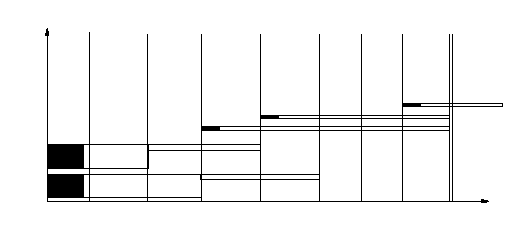
\includegraphics{figs/NDVI-N-3.fig.eps}%
\end{picture}%
\setlength{\unitlength}{4144sp}%
%
\begingroup\makeatletter\ifx\SetFigFontNFSS\undefined%
\gdef\SetFigFontNFSS#1#2#3#4#5{%
  \reset@font\fontsize{#1}{#2pt}%
  \fontfamily{#3}\fontseries{#4}\fontshape{#5}%
  \selectfont}%
\fi\endgroup%
\begin{picture}(3717,1569)(-14,-661)
\put(  1,-169){\makebox(0,0)[lb]{\smash{{\SetFigFontNFSS{5}{6.0}{\familydefault}{\mddefault}{\updefault}{\color[rgb]{0,0,0}\im{VIS}}%
}}}}
\put(1036,749){\makebox(0,0)[lb]{\smash{{\SetFigFontNFSS{5}{6.0}{\familydefault}{\mddefault}{\updefault}{\color[rgb]{0,0,0}$|_\ps{NA'}$}%
}}}}
\put(586,749){\makebox(0,0)[lb]{\smash{{\SetFigFontNFSS{5}{6.0}{\familydefault}{\mddefault}{\updefault}{\color[rgb]{0,0,0}$|_\ps{NA'}$}%
}}}}
\put(2341,749){\makebox(0,0)[lb]{\smash{{\SetFigFontNFSS{5}{6.0}{\familydefault}{\mddefault}{\updefault}{\color[rgb]{0,0,0}$|_\ps{NA}$}%
}}}}
\put(2656,749){\makebox(0,0)[lb]{\smash{{\SetFigFontNFSS{5}{6.0}{\familydefault}{\mddefault}{\updefault}{\color[rgb]{0,0,0}$|_\ps{NA}$}%
}}}}
\put(2971,749){\makebox(0,0)[lb]{\smash{{\SetFigFontNFSS{5}{6.0}{\familydefault}{\mddefault}{\updefault}{\color[rgb]{0,0,0}$f(\im{VIS},\im{IR})$}%
}}}}
\put(1441,749){\makebox(0,0)[lb]{\smash{{\SetFigFontNFSS{5}{6.0}{\familydefault}{\mddefault}{\updefault}{\color[rgb]{0,0,0}$\bigoplus\ps{N_{4\times4}}$}%
}}}}
\put(1846,749){\makebox(0,0)[lb]{\smash{{\SetFigFontNFSS{5}{6.0}{\familydefault}{\mddefault}{\updefault}{\color[rgb]{0,0,0}$\bigoplus\ps{N_{4\times4}}$}%
}}}}
\put(1801,-646){\makebox(0,0)[lb]{\smash{{\SetFigFontNFSS{5}{6.0}{\familydefault}{\mddefault}{\updefault}{\color[rgb]{0,0,0}Time}%
}}}}
\put(136,119){\rotatebox{90.0}{\makebox(0,0)[lb]{\smash{{\SetFigFontNFSS{5}{6.0}{\familydefault}{\mddefault}{\updefault}{\color[rgb]{0,0,0}Size}%
}}}}}
\put(  1,-376){\makebox(0,0)[lb]{\smash{{\SetFigFontNFSS{5}{6.0}{\familydefault}{\mddefault}{\updefault}{\color[rgb]{0,0,0}\im{IR}}%
}}}}
\put(3421,299){\makebox(0,0)[lb]{\smash{{\SetFigFontNFSS{5}{6.0}{\familydefault}{\mddefault}{\updefault}{\color[rgb]{0,0,0}\im{Q}}%
}}}}
\end{picture}%
  
  \caption{\ac{QEG} for query \qry{C} with neighborhood operation}
  \label{fig:qep-c}
\end{figure}

Table~\ref{tab:ndvi-N} shows the associated costs for this query.  The
neighborhood operation reduces costs for later operations in that for
every four rows that are input to the $\oplus \ps{N_{4\times 4}}$
operation, only one row is output and with only one fourth of the
number of pixels in the row.  This also means that although there are
more operators with a neighborhood operation, there are also savings
in the execution time due to the changes in the point set.
%
\begin{table}
  \centering
  \caption{Cost summary for query \qry{C} with neighborhood operation}
  \begin{tabular}{c|c}
    Model & Cost \\
    \hline \hline
    Execution & $2 s/h C_{M} + 2 s/h C_{N_{4\times 4}} + 3(s/h)(n/h)C_{\gamma} + 4 C_{|}$ \\
    Creation  & $\approx 3(s/h)$ \\
    Max Size  & $max(2,3s)$ \\
    Size-Time & $3(s/h)C_{M} + 3(s/h)(n/h)C_{\gamma} + (3+s+4(s/h))C_{|} + (3s+3(s/h))C_{N_{4\times 4}}$ 
  \end{tabular}
  \label{tab:ndvi-N}
\end{table}

No requirements on the specific way the neighborhood operations are
implemented is assumed in the above formulations.  In
Section~\ref{sec:nbr-multi}, the neighborhood operation is decomposed
into a set of operators as a way to increase sharing of intermediate
data in a multi-query operation.  The implementation described there
does not affect the constraints to creating a \ac{QEG} described in
this section.

\subsection{Spatial Transforms}
\label{sec:trans-op}

The final operation that is available in the query interface of
Section~\ref{sec:wms-queries} is composition, or spatial transform.
An example of this is Query~\qry{D}, which has the same formulation
as Query~\qry{C} but with an additional step of projecting the data to a
new coordinate system.  This more complete query is the final example.  

The most common spatial transformation converts the satellite point
set to the point set grid requested by a query.  Each query can
specify pixel locations and resolutions that differ from the input
images.  Transformations perform this conversion.  The transformation
definition requires that the image \im{a} be defined at arbitrary
points and not only at the original satellite pixel locations.  This
can be accomplished by extending a physical image to one where all
points are defined in some interpolated manner from the original
satellite values.  Figure~\ref{fig:interpolate} shows this
interpolation technique.  In this example, bi-linear interpolation
extends an image to supply arbitrary pixel values based on a linear
combination of the surrounding 4 pixels in the
image~\cite{wiki06}.  Other methods common in remote sensing
include nearest-neighbor techniques, where only the closest pixel
value is used, and bi-cubic convolution~\cite{wiki06}, where a
window of nine pixel values is used.

\begin{figure}[htb]
  \centering
  \psset{unit=1.6}
  \begin{FramePic}[2,2]
    \roi(0.3,0.45)(1.3,1.45){}
    \newpsstyle{pc}{linecolor=gray}
    \psline[style=pc]{->}(0.5,0.5)(0.8,0.95)
    \psline[style=pc]{->}(1.5,0.5)(0.8,0.95)
    \psline[style=pc]{->}(1.5,1.5)(0.8,0.95)
    \psline[style=pc]{->}(0.5,1.5)(0.8,0.95)
  \end{FramePic}
  \caption{Image interpolation for spatial transforms, $\im{a} \circ f$}
 \label{fig:interpolate}
\end{figure} 

Section~\ref{sec:rewrites} describes how spatial transforms can be
represented as a restriction operator followed by a composition
operator, by performing a reverse transform of the final point set.
This allows a restriction to be added into the single query.  For a
\ac{WMS} based query, the only restriction specified is in terms of
the final coordinate system, so this step is required to determine a
restriction operator for the query.

The \ac{WMS} based query formulation does not explicitly define the
order of operations, and there is some flexibility in interpretation.
In general, the best practice is to carry out all averaging and
induced operations before any spatial transformations.  This insures
retaining radiometric values as close as possible to those measured by
the \ac{RSI} instrument.  In practice, however, the transformation is
sometimes a first step in processing \ac{RSI} data.  This is primarily
because of the advantage of working in a standard coordinate system,
particularly when combining \ac{RSI} data with other \ac{GIS} data
sets.

%~\cite{?}.  
The required implicit interpolation step for performing a
transformation works best when the composed point set has a comparable
resolution to the input point set.  This means that wherever the
spatial transform is performed, the resolution of the resultant point
set should match the input point set resolution as closely as possible.
If the transformation is performed as the last step, then the
resolution of the final point set is matched to the averaging step in
the \ac{GOES} coordinate system.  If the transform is performed first,
the point set is matched to the incoming channel point set resolution.

A few other processing orders are possible as well.
Figure~\ref{fig:qep-transform} shows some \acp{QEG} for Query~\qry{D}
with the spatial transformation in different locations.  The figures
show a removal of the last restriction in query~\qry{C}.  Unlike the
previous example, this restriction is not required to match the point
set requested by the \ac{WMS} query.  That role is instead handled
with the transform step.  Since the selectivity of these restrictions
are nearly one, removing these operators does not significantly
increase the number of rows in entering the final operation.

\begin{figure}[htb]
  \centering
  \subfigure[Transform last]{
  \pstree[treemode=U,nodesep=2pt,levelsep=30pt]{\TR{Q}}
  {
    \pstree[treemode=U]{\Tcircle{$\circ LL$}}
    {
      \pstree[treemode=U]{\Tcircle{$f()$}}
      {      
        \pstree[treemode=U]{\Tb{$\oplus\pt{N_{4\times4}}$}}
        {
          \pstree[treemode=U]{\Tb{$|_{NA'}$}}{\TR[name=C1]{\im{C1}}}
        }
        \pstree[treemode=U]{\Tb{$\oplus\pt{N_{4\times4}}$}}
        {
          \pstree[treemode=U]{\Tb{$|_{NA'}$}}{\TR[name=C1]{\im{C2}}}
        }
      }
    }
  }
}
  \quad
  \subfigure[Transform after averaging]{
  \pstree[treemode=U,nodesep=2pt,levelsep=30pt]{\TR{Q}}
  {
    \pstree[treemode=U]{\Tcircle{$f()$}}
    {      
      \pstree[treemode=U]{\Tcircle{$\circ LL$}}
      {
        \pstree[treemode=U]{\Tb{$\oplus\pt{N_{4\times4}}$}}
        {
          \pstree[treemode=U]{\Tb{$|_{NA'}$}}{\TR[name=C1]{\im{C1}}}
        }
      }
      \pstree[treemode=U]{\Tcircle{$\circ LL$}}
      {
        \pstree[treemode=U]{\Tb{$\oplus\pt{N_{4\times4}}$}}
        {
          \pstree[treemode=U]{\Tb{$|_{NA'}$}}{\TR[name=C1]{\im{C2}}}
        }
      }
    }
  }
}
\quad
  \subfigure[Transform first]{
  \pstree[treemode=U,nodesep=2pt,levelsep=30pt]{\TR{Q}}{
    \pstree[treemode=U]{\Tb{$|_{NA}$}}
    {
      \pstree[treemode=U]{\Tcircle{$f()$}}
      {      
        \pstree[treemode=U]{\Tb{$\oplus\pt{N_{4\times4}}$}}
        {
          \pstree[treemode=U]{\Tcircle{$\circ LL$}}
          {
            \pstree[treemode=U]{\Tb{$|_{NA'}$}}{\TR[name=C1]{\im{C1}}}
          }
        }
        \pstree[treemode=U]{\Tb{$\oplus\pt{N_{4\times4}}$}}
        {
          \pstree[treemode=U]{\Tcircle{$\circ LL$}}
          {
            \pstree[treemode=U]{\Tb{$|_{NA'}$}}{\TR[name=C1]{\im{C2}}}
          }
        }
      }
    }
  }
}
\caption{Potential \acp{QEG} for query \qry{D} }
  \label{fig:qep-transform}
\end{figure}


In terms of defining costs for each of these \acp{QEG}, it is clear
from the formulations that the spatial transform is simply an added
cost to the previous model for query~\qry{C}.  Also,
Table~\ref{tab:operator-cost} shows the cost is a function of the
number of rows sent through the operator.  Though the order of the
operators does affect the point sets that are in the plan--for example
moving the spatial transform to the front of the \ac{QEG} does imply
all point sets after this are in the new coordinate system--the
requirement that resolutions match between point sets means that the
number of rows in the point sets does not change dramatically from one
coordinate system to the next.

All of the above considerations imply that locating this operator at
the end of the \ac{QEG} will result in the least cost, or at worst a
reasonable approximation.  This limits the number of row tuples
entered into the operator, and also reduces the constant on the size
of the operator as well.  In addition, Section~\ref{sec:multi-opt}
uses this location for the to improve sharing of data for multi-query
optimizations.  Figure~\ref{fig:qep-d} shows the graphical cost model
for this formulation.

\begin{figure}[htb]
  \centering
  \pstree[treemode=U,nodesep=2pt,levelsep=30pt]{\TR{Q}}
  {
    \pstree[treemode=U]{\Tcircle{$\circ LL$}}
    {
      \pstree[treemode=U]{\Tcircle{$f()$}}
      {      
        \pstree[treemode=U]{\Tb{$\oplus\pt{N_{4\times4}}$}}
        {
          \pstree[treemode=U]{\Tb{$|_{NA'}$}}{\TR[name=C1]{\im{C1}}}
        }
        \pstree[treemode=U]{\Tb{$\oplus\pt{N_{4\times4}}$}}
        {
          \pstree[treemode=U]{\Tb{$|_{NA'}$}}{\TR[name=C1]{\im{C2}}}
        }
      }
    }
  }
  \quad
  \begin{picture}(0,0)%
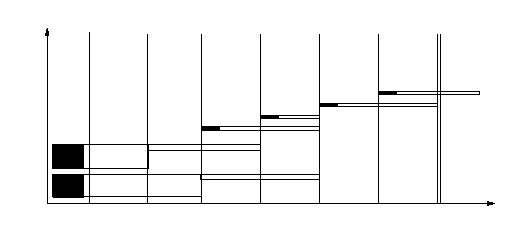
\includegraphics{figs/NDVI-NT.fig.eps}%
\end{picture}%
\setlength{\unitlength}{4144sp}%
%
\begingroup\makeatletter\ifx\SetFigFontNFSS\undefined%
\gdef\SetFigFontNFSS#1#2#3#4#5{%
  \reset@font\fontsize{#1}{#2pt}%
  \fontfamily{#3}\fontseries{#4}\fontshape{#5}%
  \selectfont}%
\fi\endgroup%
\begin{picture}(3672,1569)(-14,-661)
\put(  1,-169){\makebox(0,0)[lb]{\smash{{\SetFigFontNFSS{5}{6.0}{\familydefault}{\mddefault}{\updefault}{\color[rgb]{0,0,0}\im{VIS}}%
}}}}
\put(1036,749){\makebox(0,0)[lb]{\smash{{\SetFigFontNFSS{5}{6.0}{\familydefault}{\mddefault}{\updefault}{\color[rgb]{0,0,0}$|_\ps{NA'}$}%
}}}}
\put(586,749){\makebox(0,0)[lb]{\smash{{\SetFigFontNFSS{5}{6.0}{\familydefault}{\mddefault}{\updefault}{\color[rgb]{0,0,0}$|_\ps{NA'}$}%
}}}}
\put(1441,749){\makebox(0,0)[lb]{\smash{{\SetFigFontNFSS{5}{6.0}{\familydefault}{\mddefault}{\updefault}{\color[rgb]{0,0,0}$\bigoplus\ps{N_{4\times4}}$}%
}}}}
\put(1846,749){\makebox(0,0)[lb]{\smash{{\SetFigFontNFSS{5}{6.0}{\familydefault}{\mddefault}{\updefault}{\color[rgb]{0,0,0}$\bigoplus\ps{N_{4\times4}}$}%
}}}}
\put(1801,-646){\makebox(0,0)[lb]{\smash{{\SetFigFontNFSS{5}{6.0}{\familydefault}{\mddefault}{\updefault}{\color[rgb]{0,0,0}Time}%
}}}}
\put(136,119){\rotatebox{90.0}{\makebox(0,0)[lb]{\smash{{\SetFigFontNFSS{5}{6.0}{\familydefault}{\mddefault}{\updefault}{\color[rgb]{0,0,0}Size}%
}}}}}
\put(  1,-376){\makebox(0,0)[lb]{\smash{{\SetFigFontNFSS{5}{6.0}{\familydefault}{\mddefault}{\updefault}{\color[rgb]{0,0,0}\im{IR}}%
}}}}
\put(2341,659){\makebox(0,0)[lb]{\smash{{\SetFigFontNFSS{5}{6.0}{\familydefault}{\mddefault}{\updefault}{\color[rgb]{0,0,0}$f(\im{VIS},\im{IR})$}%
}}}}
\put(2791,749){\makebox(0,0)[lb]{\smash{{\SetFigFontNFSS{5}{6.0}{\familydefault}{\mddefault}{\updefault}{\color[rgb]{0,0,0}$\circ LL$}%
}}}}
\put(3286,389){\makebox(0,0)[lb]{\smash{{\SetFigFontNFSS{5}{6.0}{\familydefault}{\mddefault}{\updefault}{\color[rgb]{0,0,0}\im{Q}}%
}}}}
\end{picture}%
  
\caption{\ac{QEG} for query \qry{D} }
  \label{fig:qep-d}
\end{figure}

Table~\ref{tab:ndvi-NT} shows the final equations for the cost of a
complete query.  This shows the optimization plan for any general
query using the \ac{WMS} query formulation.
%
\begin{table}
  \centering
  \caption{Cost summary for query~\qry{D}}
  \begin{tabular}{c|c}
    Model & Cost \\
    \hline \hline
    Execution & $4 s/h C_{M} + 2 s/h C_{N_{4\times 4}} + 3(s/h)(n/h)C_{\gamma} + 2 C_{|} + (s/h)C_{\circ LL}$ \\
    Creation & $\approx 4(s/h)$ \\
    Max Size & $max(2,3s)$ \\
    Size-Time & $4(s/h)C_{M} + (3s+3(s/h))C_{N_{4\times 4}}+ (3+s)C_{|} + 3(s/h)(n/h)C_{\gamma} + (s/h)C_{\circ LL}$ 
  \end{tabular}
  \label{tab:ndvi-NT}
\end{table}

\subsection{Building a Single \acl{QEP}}
\label{sec:single-plan}

Building upon the previous sections, a simple methodology can be
defined for single query optimization in a very straightforward
manner.  The methodology does not change from query to query.  It is a
heuristic approach only in the sense that some particular queries
could have a moderately smaller cost by eliminating restrictions or
reordering operations. For example, a query involving 5 channels on
nearly the entire hemisphere might be slightly faster if the entire
hemisphere were processed and only one restriction applied to the
final result, as opposed to applying 5 restrictions to no or little
effect.  Even in such cases the heuristic is a reasonable alternative.

Section~\ref{sec:multi} will develop a specialized realization of the
neighborhood operation for multi-query optimization.  One result of
this will be that all queries, even those without a specified
coordinate system, will end with a transformation step even if the
requested coordinate system is in the original \ac{GOES} system.
Therefore, the steps below are valid for all input \ac{WMS} queries.

The following rules are used to optimize a single query:

\begin{enumerate}

\item The specification of the point set in the \ac{WMS} query is
  defined in the final coordinate system.  This point set is
  transformed to the \ac{GOES} perspective coordinate system including
  consideration of the pixel resolution.  This transform also defines
  the query restriction in the \ac{GOES} coordinate system.

\item If the query is for a specified derived product available
  through the \ac{WMS} interface, all input image channels required
  for that product are identified.

\item The query restriction is applied to all identified raw image channels.

\item The input channel(s) are averaged to the resolution appropriate
  for the query, as specified by the \ac{GOES} coordinate point set.

\item If the query is a derived product, a processing node is added to
  perform that calculation.  All image channels for the product are
  directed through this node.

\item The resultant image is transformed to the final coordinate
  system and point set as requested by the query.

\end{enumerate}

The resultant \ac{QEG} will always resemble the organization shown in
Figure~\ref{fig:qep-d}.

\section{Multi-Query Optimization}
\label{sec:multi-opt}

In a typical \ac{DBMS}, once the individual queries are rewritten to
optimize their individual execution, they are executed without regard
for other queries in the system.  For the \ac{DSMS}, however, queries
are often long running and it makes sense to optimize on multiple
active queries in the system.  This is especially true for queries on
\ac{RSI} where there exist opportunities to share operators as well as
intermediate results among queries that share common products and
point sets.

As an example, multi-query optimization techniques are explored for
the first four example queries from Table~\ref{tab:ref-queries},
replicated below in Table~\ref{tab:multi-example}.  The first four
queries are chosen since they share many components and offer a good
example for multi-query optimization.
%
\begin{table}[htb]
  \centering
  \caption{Example queries}
  \begin{tabular}[b]{c|c|c|c|c|c}
    {\bf Q } & {\bf Product} & {\bf \ac{ROI}} & {\bf Time} & {\bf Projection} & {\bf Resolution} \\
    \hline \hline
    \qry{A} & $C1$ & Mexico & Always & GOES &$\approx$\unit[1]{km$^2$} \\
    \qry{B} & $C1$ & N. America & Always & Lat/Long & $\approx$\unit[4]{km$^2$} \\
    \qry{C} & NDVI$(C1,C2)$ & N. America & Always & GOES & $\approx$\unit[4]{km$^2$} \\
    \qry{D} & NDVI$(C1,C2)$ & Hemisphere & Always & Lat/Long & $\approx$\unit[8]{km$^2$} \\
  \end{tabular}
  \label{tab:multi-example}
\end{table}

Figure~\ref{fig:qeg-no-opt} shows these queries all rewritten to the
processing order derived from the single query optimization of
Section~\ref{sec:single-opt}.  Determining costs for this set of
queries would entail summarizing the costs for each individual query.
In the case of \emph{Execution} and \emph{Creation}, this cost is
independent of the order of execution.  The \emph{Max-Size}, and
\emph{Size-Time} cost models are dependent on the order of processing
steps, as both are affected by the active number of tuples from the
streams in the system.

\begin{figure}[htb]
  \centering

    % A
    \pstree[treemode=U,nodesep=2pt,levelsep=30pt]{\TR{\qry{A}}}
    {
      \pstree{\TR{}}
      {
        \pstree{\TR{}}
        {      
          \pstree{\TR{}}
          {
            \pstree{\Tb[name=QAC1]{$|_{MX}$}}
            {
              \TR[name=C1]{\im{C1}}
            }
          }
        }
      }
    }
    % B
    \pstree[treemode=U,nodesep=2pt,levelsep=30pt]{\TR{\qry{B}}}
    {
      \pstree{\Tcircle{$\circ LL$}}
      {
        \pstree{\TR{}}
        {      
          \pstree{\Tb{$\oplus\pt{N_{4\times4}}$}}
          {
            \pstree{\Tb[name=QBC1]{$|_{NA'}$}}
            {
              \ncline{C1}{QBC1}
%              \TR[name=C1]{\im{C1}}
            }
          }
        }
      }
    }
    % C
    \pstree[treemode=U,nodesep=2pt,levelsep=30pt]{\TR{\qry{C}}}
    {
      \pstree{\TR{}}
      {
        \pstree{\Tcircle{$f()$}}
        {      
          \pstree{\Tb{$\oplus\pt{N_{4\times4}}$}}
          {
            \pstree{\Tb[name=QCC1]{$|_{NA'}$}}
            {
              \ncline{C1}{QCC1}
%              \TR[name=C1]{\im{C1}}
            }
          }
          \pstree{\Tb{$\oplus\pt{N_{4\times4}}$}}
          {
            \pstree{\Tb[name=QCC2]{$|_{NA'}$}}
            {
%              \ncline{C2}{QCC2}
              \TR[name=C2]{\im{C2}}
            }
          }
        }
      }
    }
    % D
    \pstree[treemode=U,nodesep=2pt,levelsep=30pt]{\TR{\qry{D}}}
    {
      \pstree{\Tcircle{$\circ LL$}}
      {
        \pstree{\Tcircle{$f()$}}
        {      
          \pstree{\Tb{$\oplus\pt{N_{8 \times 8}}$}}
          {
            \pstree{\Tb[name=QDC1]{$|_{HEMI'}$}}
            {
              \ncline{C1}{QDC1}
%              \TR[name=C1]{\im{C1}}
            }
          }
          \pstree{\Tb{$\oplus\pt{N_{8 \times 8}}$}}
          {
            \pstree{\Tb[name=QDC2]{$|_{HEMI'}$}}
            {
              \ncline{C2}{QDC2}
%              \TR[name=C2]{\im{C2}}
            }
          }
        }
      }
    }

  \caption{Unoptimized \ac{QEG} for queries \qry{A},\qry{B},\qry{C}, and \qry{D}}
  \label{fig:qeg-no-opt}
\end{figure}

Before investigating these costs, however, a few optimizations will be
applied to this set of queries.  The first thing to notice about the
above \ac{QEG} is that all queries start with a restriction operator
on one or more input image channels, all having the same input stream.
A more efficient method is to design a restriction operator developed
for multiple queries.  Table~\ref{tab:operator-cost}, anticipated a
cost savings in combining restrictions. Chapter~\ref{cha:dct} will
develop an index, the \acf{DCT}, developed specifically for
restriction operations on streaming \ac{RSI} data.  Leaving the
implementation until that chapter, the previous set of queries can be
rewritten using two shared restriction operators.
Figure~\ref{fig:qeg-share-restrictions} shows the new \ac{QEG} with
this addition.  A single restriction operation is now used and
multiple streams are output, each with their individually defined
restrictions.  As in the case of a single restriction, the
\emph{row-scan} ordering of the data allows for all restrictions to be
implemented without the creation of any new row tuples of data.

\begin{figure}[htb]
  \centering

    % A
    \pstree[treemode=U,nodesep=2pt,levelsep=30pt]{\TR{\qry{A}}}
    {
      \pstree{\TR{}}
      {
        \pstree{\TR{}}
        {      
          \pstree{\TR{}}
          {
            \pstree{\Tb[name=RC1]{$|_{MX,NA,NA',HEMI'}$}}
            {
              \TR[name=C1]{\im{C1}}
            }
          }
        }
      }
    }
    % B
    \pstree[treemode=U,nodesep=2pt,levelsep=30pt]{\TR{\qry{B}}}
    {
      \pstree{\Tcircle{$\circ LL$}}
      {
        \pstree{\TR{}}
        {      
          \pstree{\Tb[name=QBN1]{$\oplus\pt{N_{4\times4}}$}}
          {
            \ncline{RC1}{QBN1}
          }
        }
      }
    }
    % C
    \pstree[treemode=U,nodesep=2pt,levelsep=30pt]{\TR{\qry{C}}}
    {
      \pstree{\TR{}}
      {
        \pstree{\Tcircle{$f()$}}
        {      
          \pstree{\Tb[name=QCN1]{$\oplus\pt{N_{4\times4}}$}}
          {
            \ncline{RC1}{QCN1}
          }
          \pstree{\Tb{$\oplus\pt{N_{4\times4}}$}}
          {
            \pstree{\Tb[name=RC2]{$|_{NA,HEMI'}$}}
            {
              \TR[name=C2]{\im{C2}}
            }
          }
        }
      }
    }
    % D
    \pstree[treemode=U,nodesep=2pt,levelsep=30pt]{\TR{\qry{D}}}
    {
      \pstree{\Tcircle{$\circ LL$}}
      {
        \pstree{\Tcircle{$f()$}}
        {      
          \pstree{\Tb[name=QDN1]{$\oplus\pt{N_{8\times 8}}$}}
          {
            \ncline{RC1}{QDN1}
          }
          \pstree{\Tb[name=QDN2]{$\oplus\pt{N_{8 \times 8}}$}}
          {
            \ncline{RC2}{QDN2}
          }
        }
      }
    }

  \caption{\ac{QEG} for queries \qry{A},\qry{B},\qry{C}, and \qry{D}, with shared restriction}
  \label{fig:qeg-share-restrictions}
\end{figure}

Figure~\ref{fig:qeg-share-restrictions} now shows multiple queries
going into very similar neighborhood operations, covering similar
geographic regions.  Significant savings could be obtained by sharing the
intermediate results of these neighborhood operations.  However, each
query has its own averaging window size, and although these may be
very similar, there is no guarantee they are the same for any pair of
queries.  In order to allow more sharing of intermediate operations,
the neighborhood operation needs to be specialized.

\subsection{Multi-Query Neighborhood Operations}
\label{sec:nbr-multi}

Up to this point, the actual implementation of neighborhood operations
has not been discussed.  Implementation becomes an issue in the
context of multi-query optimizations since it is desirable to share
intermediate results between neighborhoods with different point set
resolutions.  The strategy chosen here is to develop a fixed number of
image resolutions that are created by progressively averaging the
\ac{RSI} images in $2 \times 2$ pixel grids.  An important component
of this strategy is that these fixed resolutions are the best
estimations of what the image radiance for the \ac{RSI} data would be
at coarser scales.  These particular resolutions will not in general
match the resolution needed by queries.  In order to calculate image
values for the point set of an individual query with its associated
pixel resolution an additional spatial transformation step is
included.  The closest averaged grid smaller then the query resolution
is chosen and, as with the previous discussion of the spatial
transform, bi-linear interpolation is used to determine the values for
the new point set.

Figure~\ref{fig:halve} shows both neighborhood operations and
interpolation techniques.  The interpolation matches that discussed
in Section~\ref{sec:trans-op}.  Involved in the neighborhood
operations is an implicit transformation to a point set which is one
fourth the size of the original.  The pixel locations are also moved
to the new center of the averaged pixels.

\begin{figure}[htb]
  \centering
 \subfigure[$\im{a} \oplus \ps{N_{/2}} \oplus \ps{N_{/2}}$]{
     {
       \psset{unit=0.4}
       \begin{FramePic}[8,8]
         \roi(0,0)(2,2){}\roi(2,0)(4,2){}\roi(4,0)(6,2){}\roi(6,0)(8,2){}
         \roi(0,2)(2,4){}\roi(2,2)(4,4){}\roi(4,2)(6,4){}\roi(6,2)(8,4){}
         \roi(0,4)(2,6){}\roi(2,4)(4,6){}\roi(4,4)(6,6){}\roi(6,4)(8,6){}
         \roi(0,6)(2,8){}\roi(2,6)(4,8){}\roi(4,6)(6,8){}\roi(6,6)(8,8){}
       \end{FramePic}
     }\quad 
     {
     \psset{unit=0.8} 
     \begin{FramePic}[4,4]
       \roi(0,0)(2,2){}\roi(2,0)(4,2){}
       \roi(0,2)(2,4){}\roi(2,2)(4,4){}
     \end{FramePic}
   }
 }\hspace*{1.5cm}
 \subfigure[$\im{a} \circ f$]{
   \psset{unit=1.6}
   \begin{FramePic}[2,2]
     \roi(0.3,0.45)(1.3,1.45){}
     \newpsstyle{pc}{linecolor=gray}
      \psline[style=pc]{->}(0.5,0.5)(0.8,0.95)
      \psline[style=pc]{->}(1.5,0.5)(0.8,0.95)
      \psline[style=pc]{->}(1.5,1.5)(0.8,0.95)
      \psline[style=pc]{->}(0.5,1.5)(0.8,0.95)
   \end{FramePic}
 }\hfill
 \caption{Image averaging and interpolation}
 \label{fig:halve}
\end{figure} 

Although there are other methods for averaging pixels, this successive
averaging is used as a simple and computationally effective method.
As is indicated from the figure, bi-linear interpolation also is a
reasonable method for point sets with a resolution with sizes up to
twice the grid resolution, as is possible with the method described
for neighborhood operations.  Once the entire neighborhood operation
is decomposed into a series of halving operations and a final
transform, they can be treated as individual operations of a query
plan.  Also, if the query contained another spatial transform, these
can be combined to a single operation, as described in
Section~\ref{sec:rewrites}.  If single query optimization were
re-investigated with this neighborhood operation implementation, the
image halving operations would float to the top of the \ac{QEG}, while
the transform would descend, perhaps joining with another spatial
transform as the last operation.

For multi-query optimization, this implementation lends itself
particularly well for sharing intermediate data within the
\ac{DSMS}. For example, in the queries~\qry{A},~\qry{B},~\qry{C}, and
\qry{D}.  After the first optimization of merging restrictions shown
in Figure~\ref{fig:qeg-share-restrictions}, most queries move next
into neighborhood operations.  Some of these cover very similar
\acp{ROI}, like queries \qry{B} and \qry{C} that have similar
point sets over North America.  Some queries are contained within
other queries, like North America being contained in the query on the
hemisphere.  Other queries share \acp{ROI}, but have resolutions that
are coarser.

Figure~\ref{fig:qeg-share-data} shows a modification to the previous
\ac{QEG} where intermediate data is shared between queries using the
described neighborhood operation.  The restriction operators are
modified as well.  Point sets are merged in the first set of
restrictions, so that overlapping \acp{ROI} are combined into a single
inclusive point set.  Next, as in the single query optimization,
streams follow with one or more image halving operations, approaching
the resolutions required by the queries.  Induced operations follow
this step.  Queries require different resolutions, and the induced
operations fork from the halving operations at various stages.
Whenever forks appear later in an image stream, a new restriction
operator is used to shuttle the required point set to the
following operators.

This optimization procedure maximizes the amount of sharing that can
occur between queries.  In fact no data shared among queries is
replicated anywhere in the stream.  As discussed in
Section~\ref{sec:multi-problems}, this is not necessarily optimal but
produces good results with queries whose \acp{ROI} tend to overlap.

\begin{figure}[htb]
  \centering
    % A
    \pstree[treemode=U,nodesep=2pt,levelsep=30pt]{\TR{\qry{A}}}
    {
      \pstree{\Tcircle{$\circ G$}}
      {
        \pstree{\TR{}}
        {      
          \pstree{\TR{}}
          {
            \pstree{\TR{}}
            {      
              \pstree{\TR{}}
              {      
                \pstree{\TR{}}
                {
                  \pstree{\Tb[name=RC1]{$|_{MX,NA+NA'+HEMI'}$}}
                  {
                    \TR[name=C1]{\im{C1}}
                  }
                }
              }
            }
          }
        }
      }
    }
    % B
    \pstree[treemode=U,nodesep=2pt,levelsep=30pt]{\TR{\qry{B}}}
    {
      \pstree{\Tcircle{$\circ LL$}}
      {
        \pstree{\TR{}}
        {      
          \pstree{\TR{}}
          {
            \pstree{\Tb[name=QBS1]{$|_{NA',NA+HEMI'}$}}
            {      
              \pstree{\Tb[name=QBN1_2]{$\oplus\pt{N_{/2}}$}}{
                \pstree{\Tb[name=QBN1]{$\oplus\pt{N_{/2}}$}}
                {
                  \ncline{RC1}{QBN1}
                }
              }
            }
          }
        }
      }
    }
    % C
    \pstree[treemode=U,nodesep=2pt,levelsep=30pt]{\TR{\qry{C}}}
    {
      \pstree{\Tcircle{$\circ G$}}
      {
        \pstree{\Tcircle[name=QCF]{$f()$}}
        {
          \ncline{QBS1}{QCF}
          \pstree{\TR{}}
          {
            \pstree{\Tb[name=QCS2]{$|_{NA,HEMI'}$}}
            {      
              \pstree{\Tb[name=QCN2_2]{$\oplus\pt{N_{/2}}$}}
              {
                \pstree{\Tb{$\oplus\pt{N_{/2}}$}}
                {
                  \pstree{\Tb[name=RC2]{$|_{NA+HEMI'}$}}
                  {
                    \TR[name=C2]{\im{C2}}
                  }
                }
              }
            }
          }
        }
      }
    }
    % D
    \pstree[treemode=U,nodesep=2pt,levelsep=30pt]{\TR{\qry{D}}}
    {
      \pstree{\Tcircle{$\circ LL$}}
      {
        \pstree{\Tcircle{$f()$}}
        {      
          \pstree{\Tb[name=QDN1_3]{$\oplus\pt{N_{/2}}$}}
          {
            \ncline{QBS1}{QDN1_3}
          }
          \pstree{\Tb[name=QDN2_3]{$\oplus\pt{N_{/2}}$}}
          {
            \ncline{QCS2}{QDN2_3}
          }
        }
      }
    }

  \caption{\ac{QEG} for queries \qry{A},\qry{B},\qry{C}, and \qry{D} optimized with shared data paths}
  \label{fig:qeg-share-data}
\end{figure}



\subsection{Building a Multi-query Optimized \acl{QEP}}
\label{sec:multi}

The example above does not demonstrate all potential paths for sharing
and optimization that can occur between multiple queries.  The actual
methodology to create the multi-query \ac{QEG} is now described.  The
execution plan in the multi-query environment is built with the goal
of using a single operator path for all queries that potentially share
intermediate results.  This includes all operators related to
resolution changes and derived operations.  The following rules are
used to optimize all queries.  Assume there is a single execution plan
that is being maintained.

\begin{enumerate}

\item Each individual query is written into the standard single query
  \ac{QEG} as discussed in Section~\ref{sec:single-plan}.

\item The neighborhood operation is decomposed into a series of
  image halving operations, followed by a final spatial
  transformation, potentially the transform originally requested by
  the query.

\item Starting from input image channel streams, the operators in the
  new query \ac{QEG} are compared to the current execution plan and
  checked for the same processing operator.

\item If the operator does not exist then it is added to execution
  plan.  In addition, a restriction to the new query's point set is
  applied before the processing node.  This effectively forks the
  stream along multiple processing paths.

\item If instead, the operator does exist, then the
  restriction associated with this node is expanded to include the new
  query if necessary.

\item The process is repeated for the next operation in the individual
  query, starting from this new current node.  This process continues
  until the final interpolation step, which is always added last into
  the execution plan, as it is not shared between multiple queries.

\end{enumerate}

Because \ac{WMS} queries are allowed to define arbitrary final point
sets, the last interpolation or projection step cannot generally be
shared among queries.  However, if queries were limited to specific
point sets, for example limiting resolutions to integer numbers of
hectares at standard postings, then an additional level of
intermediate images sharing among queries would be possible.  This
would not be a standard \ac{WMS} query, however.

The order that the queries are considered does not affect the final
\ac{QEG}, since the operators for each individual query are arranged
the same and as a result add into the multi-query plan in the same
order regardless of how the queries themselves are added.

Figures~\ref{fig:exe-plan-a},~\ref{fig:exe-plan-b},~\ref{fig:exe-plan-c}~and
~\ref{fig:exe-plan-d} progressively show the construction of the query
plan, using the same set of example queries.  These figures
demonstrate the operators, especially the restrictions, more
graphically as an attempt to demonstrate the sharing between queries.

\begin{figure}[htb]
  \centering
  \subfigure[\qry{A}]{
    \label{fig:exe-plan-a}
    \scalebox{0.8}{\begin{picture}(0,0)%
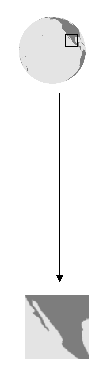
\includegraphics{figs/exe-plan-a.fig.eps}%
\end{picture}%
\setlength{\unitlength}{4144sp}%
%
\begingroup\makeatletter\ifx\SetFigFontNFSS\undefined%
\gdef\SetFigFontNFSS#1#2#3#4#5{%
  \reset@font\fontsize{#1}{#2pt}%
  \fontfamily{#3}\fontseries{#4}\fontshape{#5}%
  \selectfont}%
\fi\endgroup%
\begin{picture}(555,2665)(526,-1961)
\put(586,-1906){\makebox(0,0)[lb]{\smash{{\SetFigFontNFSS{12}{14.4}{\familydefault}{\mddefault}{\updefault}{\color[rgb]{0,0,0}$\circ G$}%
}}}}
\put(541,209){\makebox(0,0)[lb]{\smash{{\SetFigFontNFSS{12}{14.4}{\rmdefault}{\mddefault}{\updefault}{\color[rgb]{0,0,0}C1}%
}}}}
\end{picture}%
}
  }\hfill
  \subfigure[\qry{A},\qry{B}]{
    \label{fig:exe-plan-b}
    \scalebox{0.8}{\begin{picture}(0,0)%
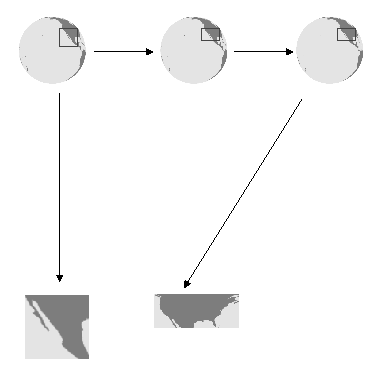
\includegraphics{figs/exe-plan-b.fig.eps}%
\end{picture}%
\setlength{\unitlength}{4144sp}%
%
\begingroup\makeatletter\ifx\SetFigFontNFSS\undefined%
\gdef\SetFigFontNFSS#1#2#3#4#5{%
  \reset@font\fontsize{#1}{#2pt}%
  \fontfamily{#3}\fontseries{#4}\fontshape{#5}%
  \selectfont}%
\fi\endgroup%
\begin{picture}(2642,2665)(526,-1961)
\put(586,-1906){\makebox(0,0)[lb]{\smash{{\SetFigFontNFSS{12}{14.4}{\familydefault}{\mddefault}{\updefault}{\color[rgb]{0,0,0}$\circ G$}%
}}}}
\put(1576,-1906){\makebox(0,0)[lb]{\smash{{\SetFigFontNFSS{12}{14.4}{\familydefault}{\mddefault}{\updefault}{\color[rgb]{0,0,0}$\circ LL$}%
}}}}
\put(2656,209){\makebox(0,0)[lb]{\smash{{\SetFigFontNFSS{12}{14.4}{\familydefault}{\mddefault}{\updefault}{\color[rgb]{0,0,0}/2}%
}}}}
\put(1621,209){\makebox(0,0)[lb]{\smash{{\SetFigFontNFSS{12}{14.4}{\familydefault}{\mddefault}{\updefault}{\color[rgb]{0,0,0}/2}%
}}}}
\put(541,209){\makebox(0,0)[lb]{\smash{{\SetFigFontNFSS{12}{14.4}{\familydefault}{\mddefault}{\updefault}{\color[rgb]{0,0,0}C1}%
}}}}
\end{picture}%
}
  }\hfill
  \subfigure[\qry{A},\qry{B},\qry{C}]{
  \label{fig:exe-plan-c}
    \scalebox{0.8}{\begin{picture}(0,0)%
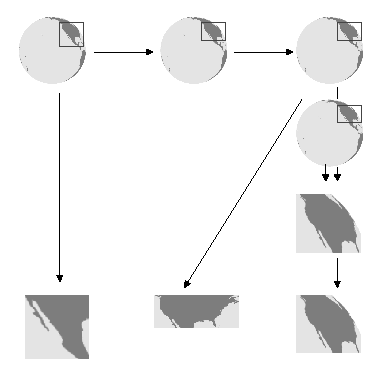
\includegraphics{figs/exe-plan-c.fig.eps}%
\end{picture}%
\setlength{\unitlength}{4144sp}%
%
\begingroup\makeatletter\ifx\SetFigFontNFSS\undefined%
\gdef\SetFigFontNFSS#1#2#3#4#5{%
  \reset@font\fontsize{#1}{#2pt}%
  \fontfamily{#3}\fontseries{#4}\fontshape{#5}%
  \selectfont}%
\fi\endgroup%
\begin{picture}(2642,2679)(526,-1975)
\put(1576,-1906){\makebox(0,0)[lb]{\smash{{\SetFigFontNFSS{12}{14.4}{\familydefault}{\mddefault}{\updefault}{\color[rgb]{0,0,0}$\circ LL$}%
}}}}
\put(586,-1906){\makebox(0,0)[lb]{\smash{{\SetFigFontNFSS{12}{14.4}{\familydefault}{\mddefault}{\updefault}{\color[rgb]{0,0,0}$\circ G$}%
}}}}
\put(2656,-1906){\makebox(0,0)[lb]{\smash{{\SetFigFontNFSS{12}{14.4}{\familydefault}{\mddefault}{\updefault}{\color[rgb]{0,0,0}$\circ G$}%
}}}}
\put(2656,-1096){\makebox(0,0)[lb]{\smash{{\SetFigFontNFSS{12}{14.4}{\familydefault}{\mddefault}{\updefault}{\color[rgb]{0,0,0}$f()$}%
}}}}
\put(2656,209){\makebox(0,0)[lb]{\smash{{\SetFigFontNFSS{12}{14.4}{\familydefault}{\mddefault}{\updefault}{\color[rgb]{0,0,0}/2}%
}}}}
\put(2656,-421){\makebox(0,0)[lb]{\smash{{\SetFigFontNFSS{12}{14.4}{\familydefault}{\mddefault}{\updefault}{\color[rgb]{0,0,0}C2}%
}}}}
\put(541,209){\makebox(0,0)[lb]{\smash{{\SetFigFontNFSS{12}{14.4}{\familydefault}{\mddefault}{\updefault}{\color[rgb]{0,0,0}C1}%
}}}}
\put(1621,209){\makebox(0,0)[lb]{\smash{{\SetFigFontNFSS{12}{14.4}{\familydefault}{\mddefault}{\updefault}{\color[rgb]{0,0,0}/2}%
}}}}
\end{picture}%
}
  }
  \caption{Execution plan for queries \qry{A}, \qry{B} and \qry{C}}
  \label{fig:exe-plan-abc}
\end{figure}

In Figure~\ref{fig:exe-plan-a}, the first query, A, is for the Channel
1, \ac{GOES} data over Mexico.  The query resolution is approximately
the same as the image stream, and no averaging is required.  The query
operations consist of a restriction on the Channel 1 image, and an
interpolation to the query point set.  

In Figure~\ref{fig:exe-plan-b}, query B is added, also for Channel 1.
The \ac{ROI} is North America, and here a coarser resolution
is required.  The Channel 1 image is reduced in resolution through two
halving operators.  The restriction on the original image is
expanded to include both query \acp{ROI}, but the averaging is
restricted to North America only.  This query also projects the final
product to a new coordinate system.

Figure~\ref{fig:exe-plan-c}, shows another query, C, over North
America being added, this one being a function of two input channels.
The processing nodes for averaging the channel 1 image have their
restrictions expanded to include this new \ac{ROI}.  In reality, for
\ac{GOES} data, different channels have different resolutions and
Channel 2 is already at the required resolution.  The restriction on
Channel 2 only needs to encompass this last query.  A new processing
node is added to perform the derived operation on the two images.

Figure~\ref{fig:exe-plan-d} shows query D requesting a nearly global
coverage for the same image function as query C.  This requires the
restrictions for all previous nodes to be expanded for this final
query.  Since two queries are interested in the same function, these
results are shared between the queries.

\begin{figure}[htb]
  \centering
  \scalebox{1.2}{\begin{picture}(0,0)%
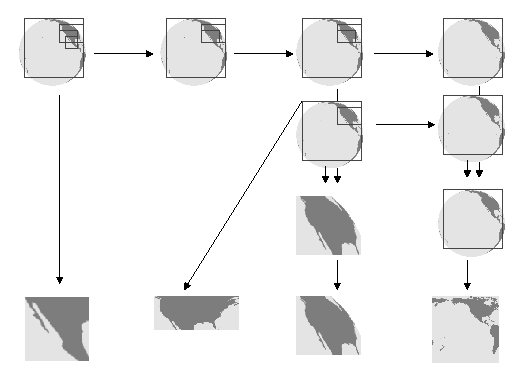
\includegraphics{figs/exe-plan-d.fig.eps}%
\end{picture}%
\setlength{\unitlength}{4144sp}%
%
\begingroup\makeatletter\ifx\SetFigFontNFSS\undefined%
\gdef\SetFigFontNFSS#1#2#3#4#5{%
  \reset@font\fontsize{#1}{#2pt}%
  \fontfamily{#3}\fontseries{#4}\fontshape{#5}%
  \selectfont}%
\fi\endgroup%
\begin{picture}(3722,2677)(526,-1961)
\put(2656,-1096){\makebox(0,0)[lb]{\smash{{\SetFigFontNFSS{12}{14.4}{\familydefault}{\mddefault}{\updefault}{\color[rgb]{0,0,0}$f(C1,C2)$}%
}}}}
\put(586,-1906){\makebox(0,0)[lb]{\smash{{\SetFigFontNFSS{12}{14.4}{\familydefault}{\mddefault}{\updefault}{\color[rgb]{0,0,0}$\circ G$}%
}}}}
\put(1576,-1906){\makebox(0,0)[lb]{\smash{{\SetFigFontNFSS{12}{14.4}{\familydefault}{\mddefault}{\updefault}{\color[rgb]{0,0,0}$\circ LL$}%
}}}}
\put(2656,-1906){\makebox(0,0)[lb]{\smash{{\SetFigFontNFSS{12}{14.4}{\familydefault}{\mddefault}{\updefault}{\color[rgb]{0,0,0}$\circ G$}%
}}}}
\put(3691,-1906){\makebox(0,0)[lb]{\smash{{\SetFigFontNFSS{12}{14.4}{\familydefault}{\mddefault}{\updefault}{\color[rgb]{0,0,0}$\circ LL$}%
}}}}
\put(2656,209){\makebox(0,0)[lb]{\smash{{\SetFigFontNFSS{12}{14.4}{\rmdefault}{\mddefault}{\updefault}{\color[rgb]{0,0,0}/2}%
}}}}
\put(3736,209){\makebox(0,0)[lb]{\smash{{\SetFigFontNFSS{12}{14.4}{\rmdefault}{\mddefault}{\updefault}{\color[rgb]{0,0,0}/2}%
}}}}
\put(2656,-421){\makebox(0,0)[lb]{\smash{{\SetFigFontNFSS{12}{14.4}{\rmdefault}{\mddefault}{\updefault}{\color[rgb]{0,0,0}C2}%
}}}}
\put(541,209){\makebox(0,0)[lb]{\smash{{\SetFigFontNFSS{12}{14.4}{\familydefault}{\mddefault}{\updefault}{\color[rgb]{0,0,0}C1}%
}}}}
\put(1621,209){\makebox(0,0)[lb]{\smash{{\SetFigFontNFSS{12}{14.4}{\familydefault}{\mddefault}{\updefault}{\color[rgb]{0,0,0}/2}%
}}}}
\put(3736,-376){\makebox(0,0)[lb]{\smash{{\SetFigFontNFSS{12}{14.4}{\familydefault}{\mddefault}{\updefault}{\color[rgb]{0,0,0}/2}%
}}}}
\put(3736,-1096){\makebox(0,0)[lb]{\smash{{\SetFigFontNFSS{12}{14.4}{\familydefault}{\mddefault}{\updefault}{\color[rgb]{0,0,0}$f(C1,C2)$}%
}}}}
\end{picture}%
}
  \caption{Execution plan for queries \qry{A}, \qry{B}, \qry{C}, and \qry{D}}
  \label{fig:exe-plan-d}
\end{figure}

The final query processing workflow combines shows all four queries
using some of the Channel 1 node, all but query A, using a common set
of averaging functions as well.  Queries C and D, also share all of
the nodes of Channel 2, as well as the output of the derived image
function.

This example also shows that the inclusion of queries with large
\acp{ROI}, like Query D, can lead to large spatial extents on many
intermediate nodes.  While driving up the total processing time, it
does allow for sharing among many queries.

\subsection{Optimization Problems}
\label{sec:multi-problems}

There are some instances where the multi-query optimizations described
do not lead to the most efficient solution.

In a few cases, the single query optimizations are not the best
starting point in optimizing multiple queries.  For example, imagine a
user launching queries for multiple products but with the same point
set.  In this case, transforming the data stream earlier results in
some savings.  Figure~\ref{fig:opt-prob-rearrange} shows an example of
three queries with three different products.  The standard
optimization strategy has an additional transform operator.  Although
there is some savings for this strategy, as was discussed in
Section~\ref{sec:trans-op}, this formulation would change the results
slightly due to the reordering of the transform and the neighborhood
operations.  Leaving the order of the single optimization \ac{QEG} in
the multi-query plan ensures the \ac{WMS} query will respond with the
same results regardless of the other queries in the system.

\begin{figure}[htb]
  \centering
  \subfigure[Standard optimization]{
  \pstree[treemode=U,nodesep=2pt,levelsep=30pt]{\TR{Q}}
  {
    \pstree[treemode=U]{\Tcircle{$\circ LL$}}
    {
      \pstree[treemode=U]{\TR{}}
      {      
        \pstree[treemode=U]{\Tb[name=C1N]{$\oplus\pt{N_{4\times4}}$}}
        {
          \pstree[treemode=U]{\Tb{$|_{NA'}$}}{\TR[name=C1]{\im{C1}}}
        }
      }
    }
  }
  \pstree[treemode=U,nodesep=2pt,levelsep=30pt]{\TR{Q2}}
  {
    \pstree[treemode=U]{\Tcircle{$\circ LL$}}
    {
      \pstree[treemode=U]{\Tcircle[name=f]{$f()$}}
      {      
        \ncline{C1N}{f}
        \pstree[treemode=U]{\Tb[name=C2N]{$\oplus\pt{N_{4\times4}}$}}
        {
          \pstree[treemode=U]{\Tb{$|_{NA'}$}}{\TR[name=C2]{\im{C2}}}
        }
      }
    }
  }
  \pstree[treemode=U,nodesep=2pt,levelsep=30pt]{\TR{Q3}}
  {
    \pstree[treemode=U]{\Tcircle[name=Q2L]{$\circ LL$}}
    {
      \ncline{C2N}{Q2L}
    }
  }
}
\quad
\subfigure[Transform first]{
  \pstree[treemode=U,nodesep=2pt,levelsep=30pt]{\TR{Q}}
  {
    \pstree[treemode=U]{\TR{}}
    {      
      \pstree[treemode=U]{\Tb[name=C1LN]{$\oplus\pt{N_{4\times4}}$}}
      {
        \pstree[treemode=U]{\Tcircle{$\circ LL$}}
        {
          \pstree[treemode=U]{\Tb{$|_{NA'}$}}{\TR[name=C1]{\im{C1}}}
        }
      }
    }
  }
  \pstree[treemode=U,nodesep=2pt,levelsep=30pt]{\TR{Q2}}
  {
    \pstree[treemode=U]{\Tcircle[name=Q2]{$f()$}}
    { 
      \ncline{C1LN}{Q2}
      \pstree[treemode=U]{\Tb[name=C2LN]{$\oplus\pt{N_{4\times4}}$}}
      {
        \pstree[treemode=U]{\Tcircle{$\circ LL$}}
        {
          \pstree[treemode=U]{\Tb{$|_{NA'}$}}{\TR[name=C1]{\im{C2}}}
        }
      }
    }
  }
  \pstree[treemode=U,nodesep=2pt,levelsep=30pt]{\TR[name=Q3]{Q3}}
  {
      \ncline{C2LN}{Q3}
  }
}
  \caption{Rearrangement of single query \ac{QEG}}
  \label{fig:opt-prob-rearrange}
\end{figure}

Another example of optimization problems is shown in the formulation
of Figure~\ref{fig:qeg-share-data}.  Here, two halving operations are
in series with no other stream using the intermediate result.  This
could more efficiently be performed with a single $N_{/4}$ operator,
and save the creation costs of those intermediate rows.  If at a
later time another query required that intermediate resolution, the
operator could be split again into two $N_{/2}$ operators in series.

The final and more troublesome problem with the multi-query
optimizations described above concerns the decision to always share
existing operators.  Since this sharing requires growing restriction
point sets to cover all queries, large numbers of the inclusive point
set might end up in no final query result.  In these cases, a better
strategy would be to not share the intermediate operation and instead
create a new operator performing the same function on a different
processing path.  Figure~\ref{fig:opt-prob-share} shows a simple
example of this problem with two small query \acp{ROI}, with a wide
separation between them.

\begin{figure}[htb]
  \centering
  \subfigure[Distant point sets]{
    \begin{picture}(0,0)%

\includegraphics{figs/share-problem.fig.eps}%
\end{picture}%
\setlength{\unitlength}{4144sp}%
%
\begingroup\makeatletter\ifx\SetFigFontNFSS\undefined%
\gdef\SetFigFontNFSS#1#2#3#4#5{%
  \reset@font\fontsize{#1}{#2pt}%
  \fontfamily{#3}\fontseries{#4}\fontshape{#5}%
  \selectfont}%
\fi\endgroup%
\begin{picture}(1575,1575)(541,-871)
\put(1711,-286){\makebox(0,0)[lb]{\smash{{\SetFigFontNFSS{12}{14.4}{\familydefault}{\mddefault}{\updefault}{\color[rgb]{0,0,0}Q2}%
}}}}
\put(946,299){\makebox(0,0)[lb]{\smash{{\SetFigFontNFSS{12}{14.4}{\familydefault}{\mddefault}{\updefault}{\color[rgb]{0,0,0}Q1}%
}}}}
\end{picture}%

  }
  \quad
  \subfigure[Standard optimization]
  {
    \pstree[treemode=U,nodesep=2pt,levelsep=30pt]{\TR{Q1}}
    {
      \pstree[treemode=U]{\Tcircle{$\circ LL$}}
      {
        \pstree[treemode=U]{\Tcircle[name=f]{$f()$}}
        {      
          \pstree[treemode=U]{\Tb{$|_{SA+RS}$}}{\TR[name=C1]{\im{C1}}}
          \pstree[treemode=U]{\Tb{$|_{SA+RS}$}}{\TR[name=C2]{\im{C2}}}
        }
      }
    }
    \pstree[treemode=U,nodesep=2pt,levelsep=30pt]{\TR{Q2}}
    {
      \pstree[treemode=U]{\Tcircle[name=Q2]{$\circ LL$}}
      {
        \ncline{f}{Q2}
      }
    }
  }
  \quad
  \subfigure[Splitting operator]
  {
    \pstree[treemode=U,nodesep=2pt,levelsep=30pt]{\TR{Q1}}
    {
      \pstree[treemode=U]{\Tcircle{$\circ LL$}}
      {
        \pstree[treemode=U]{\Tcircle[name=f]{$f()$}}
        {      
          \pstree[treemode=U]{\Tb[name=C1N]{$|_{SA,RS}$}}{\TR[name=C1]{\im{C1}}}
          \pstree[treemode=U]{\Tb[name=C2N]{$|_{SA,RS}$}}{\TR[name=C2]{\im{C2}}}
        }
      }
    }
    \pstree[treemode=U,nodesep=2pt,levelsep=30pt]{\TR{Q2}}
    {
      \pstree[treemode=U]{\Tcircle{$\circ LL$}}
      {
        \pstree[treemode=U]{\Tcircle[name=f]{$f()$}}
        {      
          \ncline{C1N}{f}
          \ncline{C2N}{f}
        }
      }
    }
  }
\caption{Inefficient sharing of intermediate results}
\label{fig:opt-prob-share}
\end{figure}

The optimization methodology described does not look at splitting
operators in such a manner.  The are two reasons for this.  First, it
is not easy to decide where to split operators in the presence of
many queries.  More importantly, alternative solutions exist for
solving this problem.  The problem is basically caused by the fact
that only rectangular point sets are defined in the restriction
operators.  Instead of splitting the operator, another solution would
involve a restriction operator that allows other point sets beyond
rectangular lattices.  If, for example, unions of rectangular regions
could be defined as a point set, then those intermediate results would
not be created and the existing optimizations would continue to offer
the best \ac{QEG} solution.  In some cases, like the experiments in
Chapter~\ref{cha:existing}, the underlying applications limit such
methods.  In other cases, like the on-line system described in
Chapter~\ref{cha:operators}, these modifications to the allowed point
set definitions could be easily included.


\section{Related Work}

The amount of research into query optimizations for relational
databases is extensive.  Because access to secondary storage is orders
of magnitudes more expensive than access to main memory, many optimization
strategies dealing only with the number of pages accessed as a cost
model are used.  Streaming databases typically work on a different
paradigm, maintaining the data and indexes in main memory, and require
a different cost model, usually based on minimizing the CPU time.  In
this context, the \ac{QEP} for a \ac{DSMS} is developed from analyzing
a number of different organizations of operators that flow together.

Optimizing streaming databases has many similarities with methods for
optimizing for multi-queries in traditional databases,
Sellis~\cite{sellis90multip-query} offering some of the earliest
examples for finding common sub-expressions.  Other studies for
multi-query optimizations through common sub-expressions
include~\cite{graef93volcan-optim,pellen97compl-trans,roy00effic}.

While multi-query optimizations have traditionally been based on
finding commonality among queries, \ac{DSMS} have concentrated effort
into systems with multiple continuous queries.  In \ac{DSMS} research
the notion of organizing multiple queries to speed up processing has
been studied under multiple conceptual definitions, including grouped
filters~\cite{madden02contin-adapt} and query
indexing~\cite{prabhakar02qindex}.

Andrade et al.~\cite{andrad03exploit-funct} described a method for
multi-query optimization of image analysis by decomposing complex
functions into more primitive operations that admit better reuse
properties, with an emphasis on aggregation functions.

All \ac{GIS} related operations have a long history.  The averaging
feature of progressively rescaling imagery by halving the spatial
resolution has been used in many applications, including
quadtrees~\cite{wiki06}, Haar wavelets~\cite{wiki06}, and image
pyramids~\cite{kropatsch91image-pyram-and-curves}.

\chapter{Multi-Query Optimization with Existing GIS Applications}
\label{cha:existing}

This chapter investigates the multi-query optimization techniques of
Chapter~\ref{cha:query} by developing a system to answer multiple user
queries on the \acf{GOES} image stream, using an existing \ac{GIS}
application as a processing framework.  

The system divides the query processing into two major components.  A
query optimizer maintains the current set of active continuous
queries. On the acquisition of a new frame of satellite images, the
optimizer produces a dynamic execution plan that is specific to the
active queries in the system. The queries are organized into a single
standard processing plan designed to share operators and intermediate
results.  The query executor rewrites this plan into a set of
geospatial processing steps and executes the plan.

The system is implemented using data from \acs{NOAA}'s \ac{GOES}.
Individual queries are defined with the \ac{WMS} query
specification. The query optimizer produces a plan that is a directed
acyclic graph with specific spatial parameters defined for each
processing node.  The query executor is implemented using the
\acf{GRASS} \ac{GIS} application~\cite{GRASS_GIS_software}.

Experimental results using predicted query patterns over the visible
hemisphere of the weather satellite indicate that developing
multi-query optimized plans can improve performance significantly when
compared to queries executed separately.


\section{Objectives}
\label{sec:ex-problem}

Chapter~\ref{cha:query} predicts savings in processing by developing a
multi-query \ac{QEP}.  How much savings is dependent on both the
implementation of the individual operators and on the make-up of the
current queries within the system.  The objective of this chapter is
to begin to quantify the savings of a multi-query \ac{QEP}, using
an existing application framework, a real \ac{RSI} image
stream, and real world query parameters.

The \ac{GIS} application framework chosen is \ac{GRASS}.
\ac{GRASS} has no notion of image streams, and like most \ac{GIS}
applications, works on discrete images in secondary storage.

The well ordered arrangement of streaming images like \ac{GOES}
weather satellite data allows natural divisions of the stream into
separate images for different channels and times.  Using these
divisions, the stream can be separated into files corresponding to
images.  \ac{GIS} data processing workflows can be applied to these
images with a number of advantages.  First, it relates to common current
practices and lends itself to simple implementations using existing
applications.  It results in processing methodologies that are
strongly connected to the current \ac{GIS} practice, including models
to develop workflows within these systems.  ESRI's model
builder~\cite{mccoy05arcgis-using} is an example of such a system.  It
is also easier to consider retrospective queries in such a system, as
the mechanism to process continuous queries is no different than
retrospective queries against previously acquired data.  Finally,
delivery mechanisms to clients launching the queries can be simplified
in this environment as well.

There are also disadvantages.  Using traditional \ac{GIS} applications
implies creation of many intermediate data layers.  This creates a
large increase in the overall size to satisfy individual query as
these intermediate images are created and used in the workflow.
Because these intermediate images rely on secondary storage, the
system can be significantly slower than a complete in-memory streaming
based system.  

The image stream used is data from \acs{NOAA}'s \ac{GOES} satellite.
The queries are on either the spectral image channels or derived
products from these channels.  The individual queries are relatively
simple and limited in expressiveness, but are designed to satisfy the
most majority of \ac{RSI} query needs.  They defined as in the
\ac{WMS} query specification.

The query optimization procedures described in Chapter~\ref{cha:query}
attempt to limit the processing time for all queries in the system.
For the \ac{RSI} queries, optimization is primarily concerned with two
goals: query writing rules to limit the amount of work done for each
query, and exploiting common subsets among individual queries active
in the system.

System performance is tested in a number of experimental designs.  All
experiments are based on query patterns meant to represent typical
access to weather satellite data.  The experiments are designed to
test some of the key areas relating to the optimization of multiple
queries, including tests on restrictions, derived products and ensembles
of queries.


\section{Prototype and Experiments}
\label{sec:experiments-gis}

The system described above has been implemented using a combination of
the \ac{GRASS}~\cite{GRASS_GIS_software} \ac{GIS} application and
supporting Unix-like tools.  \ac{GRASS} is a procedural \ac{GIS}
application that is especially well suited to raster data
manipulation.  \ac{GRASS} is developed as a series of stand-alone
programs that can be linked together for more complex operations.
\ac{GRASS} includes the notion of an active region.  This applies an
implicit restriction for most operations in \ac{GRASS}.

Because \ac{GRASS} is implemented as group of standalone applications,
the default processing environment is the command shell and standard tools are
available for programming the \ac{GIS}.  In particular, this
application uses a sophisticated \texttt{makefile} as the query plan
executor.  \texttt{Make} is designed to execute \acp{DAG}, and lends
itself well to organizing the \ac{GRASS} processes.  The query
optimizer is a separate program that organizes the multiple queries
into a single processing workflow.

The experiments were developed to replicate sets of queries made on
\ac{GOES} Imager input data and realistic \acp{ROI} for the continuous
queries.  Rather than randomly locate these \acp{ROI} throughout the
image domain, they were preferentially located around a small number
of ``hot spots'' in the hemisphere.  This more closely relates to real
world scenarios where specific parts of the \ac{RSI} data is
requested by a large numbers of users.  Although the general area of
the queries was fixed to a small number of locations, the individual
\ac{ROI} centers, total sizes and aspect ratios were varied for each
\ac{ROI}.  This corresponds to many users requesting slightly
different particulars for a general \ac{ROI}.  Some random \acp{ROI}
were also included in the experimental setup.  Table~\ref{tab:parms}
describes the parameters for the query \acp{ROI}.  The query region
parameters table lists the various general regions used in the
setup. Each general \acp{ROI} was given equal weight and the queries
were randomly distributed among them.  The \ac{ROI} variation table
shows the range of variation on the image size, location, and aspect
with respect to the selected ``hot spot''
%
\begin{table}[htb]
  \centering
  \caption{Query \ac{ROI} parameters}
    \begin{tabular}[t]{lr}
      \multicolumn{2}{c}{Query Regions} \\
      \hline \hline
      Global & GL           \\     
      Northern Hemisphere & NH \\     
      United States & US \\           
      Western Coastal & WC \\        
      Mexico & MX             \\    
      South America & SA \\
      Random & RN
    \end{tabular}
    \quad
    \begin{tabular}[t]{ll}
      \multicolumn{2}{c}{\ac{ROI} Variations} \\
      \hline \hline
      Area & 0.8-1.2 \\
      Aspect & $\pm 10\%$ \\
      Center & $\pm 10\%$ \\ 
    \end{tabular}
  \label{tab:parms}
\end{table}

Data from the \ac{GOES} satellite is received directly from a
receiving station co-located with the computer running the query
application.  \ac{GOES} scans various sections of the Earth's surface
about once every 15-30 minutes in specific frames.  Frames range in
size from \unit[100]{MB} to \unit[440]{MB}.

Query optimizations described in Chapter~\ref{cha:query} were tested
against a system running queries that were individually optimized
only.  Between 5 and 100 queries were posed against the system, and
performance measured as the total processing time for each MB of data
delivered to queries.  Various combinations of restrictions and
derived operations were performed on either single channels or all
channels in the system.  For simplicity, all queries were executed on
the default \ac{GOES} coordinate system.

Most experiments were run against a single set of \ac{GOES} Imager
data corresponding to a full disk input set taken in mid-day.  Channel
1 was about \unit[440]{MB} in size, with 10828 rows and 20792 columns
in the input image.  The other channels have coarser resolutions and
are about a quarter of the size.

Figure~\ref{fig:density} shows the distribution of the input query
\acp{ROI} over the hemisphere.  Lighter areas on the map indicate more
queries for that region.  Areas along the western seaboard are most
queried.  For 100 queries, individual pixels participate in an average
of about 28 queries, with participation in up to 66 queries for some
pixels.  The experiments were run using 5, 20, 50, and 100 individual
queries.

\begin{figure}[htb]
  \centering
  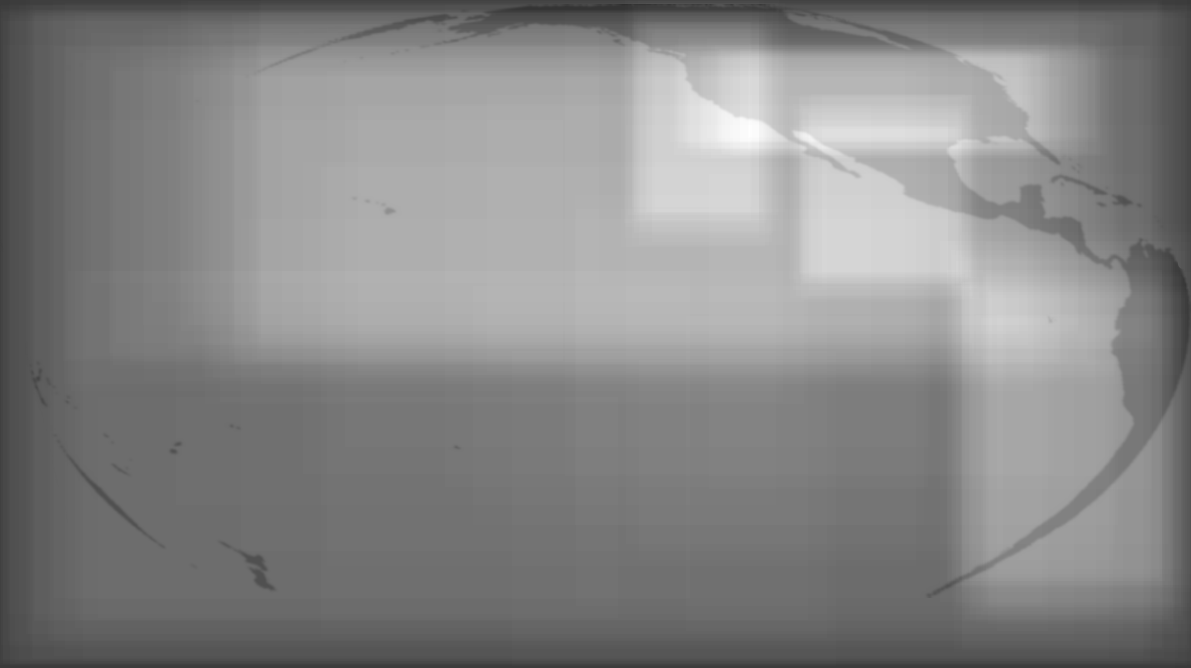
\includegraphics[width=0.8\textwidth]{figs/density/density}
  \caption{Query density}
  \label{fig:density}
\end{figure}

As the experiments show, the processing time is related also to the
final resolution of images requested by the queries.  Two sets of
query image resolutions were used in the experiments.  In both cases,
the query resolution ranged from resolutions on the scale of the
finest satellite image--channel 1, approximately \unit[1]{km}
resolution at nadir--to a resolution corresponding to a query image
width of 256 pixels, a reasonable lower bound on resolution.  The
distribution of resolutions were varied.  Both distributions weighted
the finer resolutions more then the coarser ones, but with different
scales.  Figure~\ref{fig:resolution} shows the histogram distributions
of the two example query sets.

\begin{figure}[htb]
  \centering
  \subfigure[Fine resolution]{
    \scalebox{0.9}{\begin{picture}(0,0)%
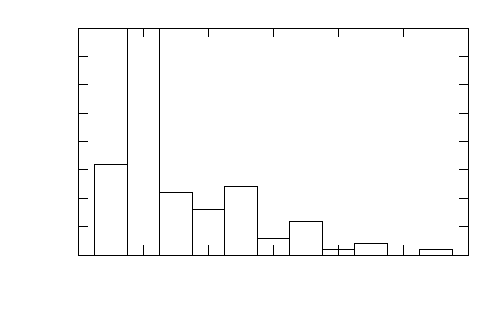
\includegraphics{grass/Q-lin.fig.eps}%
\end{picture}%
\setlength{\unitlength}{3947sp}%
%
\begingroup\makeatletter\ifx\SetFigFont\undefined%
\gdef\SetFigFont#1#2#3#4#5{%
  \reset@font\fontsize{#1}{#2pt}%
  \fontfamily{#3}\fontseries{#4}\fontshape{#5}%
  \selectfont}%
\fi\endgroup%
\begin{picture}(3747,2319)(1271,-4012)
\put(1688,-3648){\makebox(0,0)[rb]{\smash{{\SetFigFont{10}{12.0}{\familydefault}{\mddefault}{\updefault} 0}}}}
\put(1688,-3421){\makebox(0,0)[rb]{\smash{{\SetFigFont{10}{12.0}{\familydefault}{\mddefault}{\updefault} 5}}}}
\put(1688,-3194){\makebox(0,0)[rb]{\smash{{\SetFigFont{10}{12.0}{\familydefault}{\mddefault}{\updefault} 10}}}}
\put(1688,-2967){\makebox(0,0)[rb]{\smash{{\SetFigFont{10}{12.0}{\familydefault}{\mddefault}{\updefault} 15}}}}
\put(1688,-2740){\makebox(0,0)[rb]{\smash{{\SetFigFont{10}{12.0}{\familydefault}{\mddefault}{\updefault} 20}}}}
\put(1688,-2514){\makebox(0,0)[rb]{\smash{{\SetFigFont{10}{12.0}{\familydefault}{\mddefault}{\updefault} 25}}}}
\put(1688,-2287){\makebox(0,0)[rb]{\smash{{\SetFigFont{10}{12.0}{\familydefault}{\mddefault}{\updefault} 30}}}}
\put(1688,-2060){\makebox(0,0)[rb]{\smash{{\SetFigFont{10}{12.0}{\familydefault}{\mddefault}{\updefault} 35}}}}
\put(1688,-1833){\makebox(0,0)[rb]{\smash{{\SetFigFont{10}{12.0}{\familydefault}{\mddefault}{\updefault} 40}}}}
\put(1763,-3773){\makebox(0,0)[b]{\smash{{\SetFigFont{10}{12.0}{\familydefault}{\mddefault}{\updefault} 0}}}}
\put(2284,-3773){\makebox(0,0)[b]{\smash{{\SetFigFont{10}{12.0}{\familydefault}{\mddefault}{\updefault} 2}}}}
\put(2805,-3773){\makebox(0,0)[b]{\smash{{\SetFigFont{10}{12.0}{\familydefault}{\mddefault}{\updefault} 4}}}}
\put(3326,-3773){\makebox(0,0)[b]{\smash{{\SetFigFont{10}{12.0}{\familydefault}{\mddefault}{\updefault} 6}}}}
\put(3846,-3773){\makebox(0,0)[b]{\smash{{\SetFigFont{10}{12.0}{\familydefault}{\mddefault}{\updefault} 8}}}}
\put(4367,-3773){\makebox(0,0)[b]{\smash{{\SetFigFont{10}{12.0}{\familydefault}{\mddefault}{\updefault} 10}}}}
\put(4888,-3773){\makebox(0,0)[b]{\smash{{\SetFigFont{10}{12.0}{\familydefault}{\mddefault}{\updefault} 12}}}}
\put(1387,-2679){\rotatebox{90.0}{\makebox(0,0)[b]{\smash{{\SetFigFont{10}{12.0}{\familydefault}{\mddefault}{\updefault}{No. of Queries}}}}}}
\put(3325,-3960){\makebox(0,0)[b]{\smash{{\SetFigFont{10}{12.0}{\familydefault}{\mddefault}{\updefault}{Resolution}}}}}
\end{picture}%
}
  }
  \subfigure[Coarse resolution]{
    \scalebox{0.9}{\begin{picture}(0,0)%
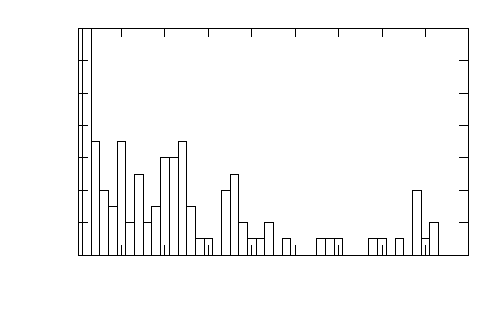
\includegraphics{grass/Q-log.fig.eps}%
\end{picture}%
\setlength{\unitlength}{3947sp}%
%
\begingroup\makeatletter\ifx\SetFigFont\undefined%
\gdef\SetFigFont#1#2#3#4#5{%
  \reset@font\fontsize{#1}{#2pt}%
  \fontfamily{#3}\fontseries{#4}\fontshape{#5}%
  \selectfont}%
\fi\endgroup%
\begin{picture}(3747,2319)(1271,-4012)
\put(1688,-3648){\makebox(0,0)[rb]{\smash{{\SetFigFont{10}{12.0}{\familydefault}{\mddefault}{\updefault} 0}}}}
\put(1688,-3389){\makebox(0,0)[rb]{\smash{{\SetFigFont{10}{12.0}{\familydefault}{\mddefault}{\updefault} 2}}}}
\put(1688,-3129){\makebox(0,0)[rb]{\smash{{\SetFigFont{10}{12.0}{\familydefault}{\mddefault}{\updefault} 4}}}}
\put(1688,-2870){\makebox(0,0)[rb]{\smash{{\SetFigFont{10}{12.0}{\familydefault}{\mddefault}{\updefault} 6}}}}
\put(1688,-2611){\makebox(0,0)[rb]{\smash{{\SetFigFont{10}{12.0}{\familydefault}{\mddefault}{\updefault} 8}}}}
\put(1688,-2352){\makebox(0,0)[rb]{\smash{{\SetFigFont{10}{12.0}{\familydefault}{\mddefault}{\updefault} 10}}}}
\put(1688,-2092){\makebox(0,0)[rb]{\smash{{\SetFigFont{10}{12.0}{\familydefault}{\mddefault}{\updefault} 12}}}}
\put(1688,-1833){\makebox(0,0)[rb]{\smash{{\SetFigFont{10}{12.0}{\familydefault}{\mddefault}{\updefault} 14}}}}
\put(1763,-3773){\makebox(0,0)[b]{\smash{{\SetFigFont{10}{12.0}{\familydefault}{\mddefault}{\updefault} 0}}}}
\put(2110,-3773){\makebox(0,0)[b]{\smash{{\SetFigFont{10}{12.0}{\familydefault}{\mddefault}{\updefault} 5}}}}
\put(2457,-3773){\makebox(0,0)[b]{\smash{{\SetFigFont{10}{12.0}{\familydefault}{\mddefault}{\updefault} 10}}}}
\put(2805,-3773){\makebox(0,0)[b]{\smash{{\SetFigFont{10}{12.0}{\familydefault}{\mddefault}{\updefault} 15}}}}
\put(3152,-3773){\makebox(0,0)[b]{\smash{{\SetFigFont{10}{12.0}{\familydefault}{\mddefault}{\updefault} 20}}}}
\put(3499,-3773){\makebox(0,0)[b]{\smash{{\SetFigFont{10}{12.0}{\familydefault}{\mddefault}{\updefault} 25}}}}
\put(3846,-3773){\makebox(0,0)[b]{\smash{{\SetFigFont{10}{12.0}{\familydefault}{\mddefault}{\updefault} 30}}}}
\put(4194,-3773){\makebox(0,0)[b]{\smash{{\SetFigFont{10}{12.0}{\familydefault}{\mddefault}{\updefault} 35}}}}
\put(4541,-3773){\makebox(0,0)[b]{\smash{{\SetFigFont{10}{12.0}{\familydefault}{\mddefault}{\updefault} 40}}}}
\put(4888,-3773){\makebox(0,0)[b]{\smash{{\SetFigFont{10}{12.0}{\familydefault}{\mddefault}{\updefault} 45}}}}
\put(1387,-2679){\rotatebox{90.0}{\makebox(0,0)[b]{\smash{{\SetFigFont{10}{12.0}{\familydefault}{\mddefault}{\updefault}{No. of Queries}}}}}}
\put(3325,-3960){\makebox(0,0)[b]{\smash{{\SetFigFont{10}{12.0}{\familydefault}{\mddefault}{\updefault}{Resolution}}}}}
\end{picture}%
}
  }
  \caption{Query resolutions}
  \label{fig:resolution}
\end{figure}


The experiments were run on a quad Intel(R) Xeon(TM) CPU
2.80GHz processor with 4GB of memory and a 3.1 TB RAID 5 filesystem
using 3ware 9500S-12 SATA-RAID


% Figure~\ref{fig:halve} shows the total cost of progressively halving
% an image, which basically shows that the first resolution change from
% $1x1$ to $2 \times 2$ dominates the cost of creating coarser representations
% of images.

% \begin{figure}[htb]
%   \centering
%   \subfigure[Progressive halving] {
%     \input{graphs/halve.fig.tex}
%     }
%     \subfigure[Cost of first halve]{
%       \input{graphs/halve_bysize.fig.tex}
%     }
%   \caption{Halving costs}
%   \label{fig:halve}
% \end{figure}

\subsection{Restrictions}

The first tests investigated only the effects of sharing intermediate
data for restrictions only.  In this example, queries were limited
to simple restrictions on image channel 1.  For the multi-query
optimization plan, this includes sharing of intermediate datasets at
the various coarser resolutions of the channel 1 data.
Figures~\ref{fig:ch1-lin}~and~\ref{fig:ch1-log} show the processing
time normalized to the total size of all query output.  In both
instances sharing intermediate data sets decreases the overall
processing time of the system.  For the finer resolution case, as the
number of queries increases, the mix of \acp{ROI} in the set becomes
fairly uniform, and the average processing time becomes fairly
constant.

\begin{figure}[htb]
  \centering
  \subfigure[Fine resolutions]{
    \label{fig:ch1-lin}
    \scalebox{0.9}{\begin{picture}(0,0)%
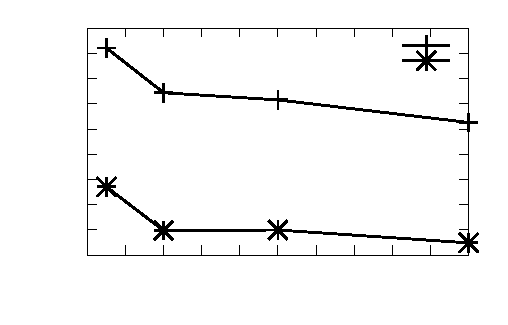
\includegraphics{grass/etc-ch1-lin/time.fig.eps}%
\end{picture}%
\setlength{\unitlength}{3947sp}%
%
\begingroup\makeatletter\ifx\SetFigFont\undefined%
\gdef\SetFigFont#1#2#3#4#5{%
  \reset@font\fontsize{#1}{#2pt}%
  \fontfamily{#3}\fontseries{#4}\fontshape{#5}%
  \selectfont}%
\fi\endgroup%
\begin{picture}(3784,2319)(1272,-4012)
\put(1763,-3648){\makebox(0,0)[rb]{\smash{{\SetFigFont{10}{12.0}{\familydefault}{\mddefault}{\updefault} 0.4}}}}
\put(1763,-3446){\makebox(0,0)[rb]{\smash{{\SetFigFont{10}{12.0}{\familydefault}{\mddefault}{\updefault} 0.5}}}}
\put(1763,-3245){\makebox(0,0)[rb]{\smash{{\SetFigFont{10}{12.0}{\familydefault}{\mddefault}{\updefault} 0.6}}}}
\put(1763,-3043){\makebox(0,0)[rb]{\smash{{\SetFigFont{10}{12.0}{\familydefault}{\mddefault}{\updefault} 0.7}}}}
\put(1763,-2841){\makebox(0,0)[rb]{\smash{{\SetFigFont{10}{12.0}{\familydefault}{\mddefault}{\updefault} 0.8}}}}
\put(1763,-2640){\makebox(0,0)[rb]{\smash{{\SetFigFont{10}{12.0}{\familydefault}{\mddefault}{\updefault} 0.9}}}}
\put(1763,-2438){\makebox(0,0)[rb]{\smash{{\SetFigFont{10}{12.0}{\familydefault}{\mddefault}{\updefault} 1}}}}
\put(1763,-2236){\makebox(0,0)[rb]{\smash{{\SetFigFont{10}{12.0}{\familydefault}{\mddefault}{\updefault} 1.1}}}}
\put(1763,-2035){\makebox(0,0)[rb]{\smash{{\SetFigFont{10}{12.0}{\familydefault}{\mddefault}{\updefault} 1.2}}}}
\put(1763,-1833){\makebox(0,0)[rb]{\smash{{\SetFigFont{10}{12.0}{\familydefault}{\mddefault}{\updefault} 1.3}}}}
\put(1838,-3773){\makebox(0,0)[b]{\smash{{\SetFigFont{10}{12.0}{\familydefault}{\mddefault}{\updefault} 0}}}}
\put(2143,-3773){\makebox(0,0)[b]{\smash{{\SetFigFont{10}{12.0}{\familydefault}{\mddefault}{\updefault} 10}}}}
\put(2448,-3773){\makebox(0,0)[b]{\smash{{\SetFigFont{10}{12.0}{\familydefault}{\mddefault}{\updefault} 20}}}}
\put(2753,-3773){\makebox(0,0)[b]{\smash{{\SetFigFont{10}{12.0}{\familydefault}{\mddefault}{\updefault} 30}}}}
\put(3058,-3773){\makebox(0,0)[b]{\smash{{\SetFigFont{10}{12.0}{\familydefault}{\mddefault}{\updefault} 40}}}}
\put(3363,-3773){\makebox(0,0)[b]{\smash{{\SetFigFont{10}{12.0}{\familydefault}{\mddefault}{\updefault} 50}}}}
\put(3668,-3773){\makebox(0,0)[b]{\smash{{\SetFigFont{10}{12.0}{\familydefault}{\mddefault}{\updefault} 60}}}}
\put(3973,-3773){\makebox(0,0)[b]{\smash{{\SetFigFont{10}{12.0}{\familydefault}{\mddefault}{\updefault} 70}}}}
\put(4278,-3773){\makebox(0,0)[b]{\smash{{\SetFigFont{10}{12.0}{\familydefault}{\mddefault}{\updefault} 80}}}}
\put(4583,-3773){\makebox(0,0)[b]{\smash{{\SetFigFont{10}{12.0}{\familydefault}{\mddefault}{\updefault} 90}}}}
\put(4888,-3773){\makebox(0,0)[b]{\smash{{\SetFigFont{10}{12.0}{\familydefault}{\mddefault}{\updefault} 100}}}}
\put(1387,-2679){\rotatebox{90.0}{\makebox(0,0)[b]{\smash{{\SetFigFont{10}{12.0}{\familydefault}{\mddefault}{\updefault}{Processing Time [$sec / MB$] }}}}}}
\put(3363,-3960){\makebox(0,0)[b]{\smash{{\SetFigFont{10}{12.0}{\familydefault}{\mddefault}{\updefault}{Number of Queries}}}}}
\put(4288,-1970){\makebox(0,0)[rb]{\smash{{\SetFigFont{10}{12.0}{\familydefault}{\mddefault}{\updefault}single}}}}
\put(4288,-2095){\makebox(0,0)[rb]{\smash{{\SetFigFont{10}{12.0}{\familydefault}{\mddefault}{\updefault}multi}}}}
\end{picture}%
}
  }
  \subfigure[Coarse resolutions]{
    \label{fig:ch1-log}
    \scalebox{0.9}{\begin{picture}(0,0)%
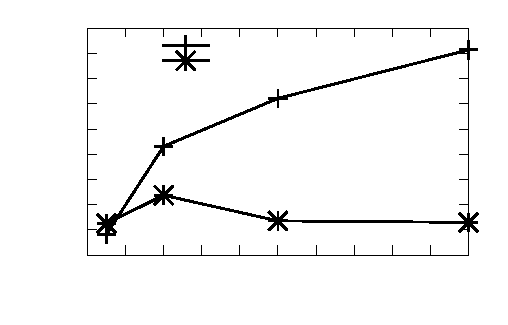
\includegraphics{grass/etc-ch1-log/time.fig.eps}%
\end{picture}%
\setlength{\unitlength}{3947sp}%
%
\begingroup\makeatletter\ifx\SetFigFont\undefined%
\gdef\SetFigFont#1#2#3#4#5{%
  \reset@font\fontsize{#1}{#2pt}%
  \fontfamily{#3}\fontseries{#4}\fontshape{#5}%
  \selectfont}%
\fi\endgroup%
\begin{picture}(3784,2319)(1272,-4012)
\put(1763,-3648){\makebox(0,0)[rb]{\smash{{\SetFigFont{10}{12.0}{\familydefault}{\mddefault}{\updefault} 0.3}}}}
\put(1763,-3446){\makebox(0,0)[rb]{\smash{{\SetFigFont{10}{12.0}{\familydefault}{\mddefault}{\updefault} 0.4}}}}
\put(1763,-3245){\makebox(0,0)[rb]{\smash{{\SetFigFont{10}{12.0}{\familydefault}{\mddefault}{\updefault} 0.5}}}}
\put(1763,-3043){\makebox(0,0)[rb]{\smash{{\SetFigFont{10}{12.0}{\familydefault}{\mddefault}{\updefault} 0.6}}}}
\put(1763,-2841){\makebox(0,0)[rb]{\smash{{\SetFigFont{10}{12.0}{\familydefault}{\mddefault}{\updefault} 0.7}}}}
\put(1763,-2640){\makebox(0,0)[rb]{\smash{{\SetFigFont{10}{12.0}{\familydefault}{\mddefault}{\updefault} 0.8}}}}
\put(1763,-2438){\makebox(0,0)[rb]{\smash{{\SetFigFont{10}{12.0}{\familydefault}{\mddefault}{\updefault} 0.9}}}}
\put(1763,-2236){\makebox(0,0)[rb]{\smash{{\SetFigFont{10}{12.0}{\familydefault}{\mddefault}{\updefault} 1}}}}
\put(1763,-2035){\makebox(0,0)[rb]{\smash{{\SetFigFont{10}{12.0}{\familydefault}{\mddefault}{\updefault} 1.1}}}}
\put(1763,-1833){\makebox(0,0)[rb]{\smash{{\SetFigFont{10}{12.0}{\familydefault}{\mddefault}{\updefault} 1.2}}}}
\put(1838,-3773){\makebox(0,0)[b]{\smash{{\SetFigFont{10}{12.0}{\familydefault}{\mddefault}{\updefault} 0}}}}
\put(2143,-3773){\makebox(0,0)[b]{\smash{{\SetFigFont{10}{12.0}{\familydefault}{\mddefault}{\updefault} 10}}}}
\put(2448,-3773){\makebox(0,0)[b]{\smash{{\SetFigFont{10}{12.0}{\familydefault}{\mddefault}{\updefault} 20}}}}
\put(2753,-3773){\makebox(0,0)[b]{\smash{{\SetFigFont{10}{12.0}{\familydefault}{\mddefault}{\updefault} 30}}}}
\put(3058,-3773){\makebox(0,0)[b]{\smash{{\SetFigFont{10}{12.0}{\familydefault}{\mddefault}{\updefault} 40}}}}
\put(3363,-3773){\makebox(0,0)[b]{\smash{{\SetFigFont{10}{12.0}{\familydefault}{\mddefault}{\updefault} 50}}}}
\put(3668,-3773){\makebox(0,0)[b]{\smash{{\SetFigFont{10}{12.0}{\familydefault}{\mddefault}{\updefault} 60}}}}
\put(3973,-3773){\makebox(0,0)[b]{\smash{{\SetFigFont{10}{12.0}{\familydefault}{\mddefault}{\updefault} 70}}}}
\put(4278,-3773){\makebox(0,0)[b]{\smash{{\SetFigFont{10}{12.0}{\familydefault}{\mddefault}{\updefault} 80}}}}
\put(4583,-3773){\makebox(0,0)[b]{\smash{{\SetFigFont{10}{12.0}{\familydefault}{\mddefault}{\updefault} 90}}}}
\put(4888,-3773){\makebox(0,0)[b]{\smash{{\SetFigFont{10}{12.0}{\familydefault}{\mddefault}{\updefault} 100}}}}
\put(1387,-2679){\rotatebox{90.0}{\makebox(0,0)[b]{\smash{{\SetFigFont{10}{12.0}{\familydefault}{\mddefault}{\updefault}{Processing Time [$sec / MB$] }}}}}}
\put(3363,-3960){\makebox(0,0)[b]{\smash{{\SetFigFont{10}{12.0}{\familydefault}{\mddefault}{\updefault}{Number of Queries}}}}}
\put(2363,-1970){\makebox(0,0)[rb]{\smash{{\SetFigFont{10}{12.0}{\familydefault}{\mddefault}{\updefault}single}}}}
\put(2363,-2095){\makebox(0,0)[rb]{\smash{{\SetFigFont{10}{12.0}{\familydefault}{\mddefault}{\updefault}multi}}}}
\end{picture}%
}
  }
  \caption{Restriction only experiment}
  \label{fig:ch1-lin-log}
\end{figure}

The savings are more dramatic for the coarser scales, primarily
because each individual query is more expensive since more averaging
needs to be done.  This is not true in the optimized case, as all the
averaging is performed one time for all queries.  It is unclear why the
processing time for the non-optimized case did not stabilize to a more
constant processing time in this example.

Overall, there is about a two fold decrease in the processing time
using multi-query optimizations.  

\subsection{Derived Products}
\label{sec:derived}

If simple restriction queries show an improvement in processing time
due to multi-query optimization, it would be expected that derived
products would show even more improvement.  This is because the
multi-query optimization saves on two levels, by avoiding image
averaging on multiple channels for each query, and by sharing the
derived product among all queries.

Two example derivative products were examined.  The first was a
normalized difference ratio, a product in Queries~\qry{C}~and~\qry{D},
discussed in Chapter~\ref{cha:query}.  This is a moderate computation.
Figure~\ref{fig:ndvi-lin} shows this experiment being run on the finer
resolution test.  As expected, the multi-query optimization runs
considerably faster then the single query optimization, by about a
factor of 3.

\begin{figure}[htb]
  \centering
  \subfigure[Image ratio, channels A and B]{
    \label{fig:ndvi-lin}
    \scalebox{0.9}{\begin{picture}(0,0)%
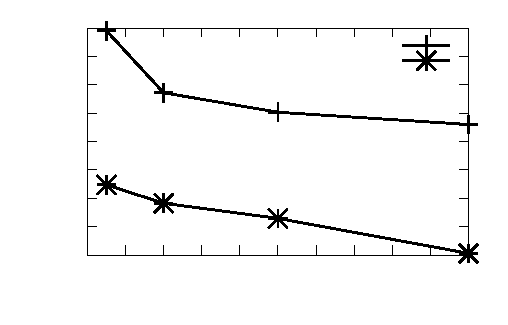
\includegraphics{grass/etc-ndvi-lin/time.fig.eps}%
\end{picture}%
\setlength{\unitlength}{3947sp}%
%
\begingroup\makeatletter\ifx\SetFigFont\undefined%
\gdef\SetFigFont#1#2#3#4#5{%
  \reset@font\fontsize{#1}{#2pt}%
  \fontfamily{#3}\fontseries{#4}\fontshape{#5}%
  \selectfont}%
\fi\endgroup%
\begin{picture}(3784,2319)(1272,-4012)
\put(1763,-3648){\makebox(0,0)[rb]{\smash{{\SetFigFont{10}{12.0}{\familydefault}{\mddefault}{\updefault} 0.4}}}}
\put(1763,-3421){\makebox(0,0)[rb]{\smash{{\SetFigFont{10}{12.0}{\familydefault}{\mddefault}{\updefault} 0.6}}}}
\put(1763,-3194){\makebox(0,0)[rb]{\smash{{\SetFigFont{10}{12.0}{\familydefault}{\mddefault}{\updefault} 0.8}}}}
\put(1763,-2967){\makebox(0,0)[rb]{\smash{{\SetFigFont{10}{12.0}{\familydefault}{\mddefault}{\updefault} 1}}}}
\put(1763,-2741){\makebox(0,0)[rb]{\smash{{\SetFigFont{10}{12.0}{\familydefault}{\mddefault}{\updefault} 1.2}}}}
\put(1763,-2514){\makebox(0,0)[rb]{\smash{{\SetFigFont{10}{12.0}{\familydefault}{\mddefault}{\updefault} 1.4}}}}
\put(1763,-2287){\makebox(0,0)[rb]{\smash{{\SetFigFont{10}{12.0}{\familydefault}{\mddefault}{\updefault} 1.6}}}}
\put(1763,-2060){\makebox(0,0)[rb]{\smash{{\SetFigFont{10}{12.0}{\familydefault}{\mddefault}{\updefault} 1.8}}}}
\put(1763,-1833){\makebox(0,0)[rb]{\smash{{\SetFigFont{10}{12.0}{\familydefault}{\mddefault}{\updefault} 2}}}}
\put(1838,-3773){\makebox(0,0)[b]{\smash{{\SetFigFont{10}{12.0}{\familydefault}{\mddefault}{\updefault} 0}}}}
\put(2143,-3773){\makebox(0,0)[b]{\smash{{\SetFigFont{10}{12.0}{\familydefault}{\mddefault}{\updefault} 10}}}}
\put(2448,-3773){\makebox(0,0)[b]{\smash{{\SetFigFont{10}{12.0}{\familydefault}{\mddefault}{\updefault} 20}}}}
\put(2753,-3773){\makebox(0,0)[b]{\smash{{\SetFigFont{10}{12.0}{\familydefault}{\mddefault}{\updefault} 30}}}}
\put(3058,-3773){\makebox(0,0)[b]{\smash{{\SetFigFont{10}{12.0}{\familydefault}{\mddefault}{\updefault} 40}}}}
\put(3363,-3773){\makebox(0,0)[b]{\smash{{\SetFigFont{10}{12.0}{\familydefault}{\mddefault}{\updefault} 50}}}}
\put(3668,-3773){\makebox(0,0)[b]{\smash{{\SetFigFont{10}{12.0}{\familydefault}{\mddefault}{\updefault} 60}}}}
\put(3973,-3773){\makebox(0,0)[b]{\smash{{\SetFigFont{10}{12.0}{\familydefault}{\mddefault}{\updefault} 70}}}}
\put(4278,-3773){\makebox(0,0)[b]{\smash{{\SetFigFont{10}{12.0}{\familydefault}{\mddefault}{\updefault} 80}}}}
\put(4583,-3773){\makebox(0,0)[b]{\smash{{\SetFigFont{10}{12.0}{\familydefault}{\mddefault}{\updefault} 90}}}}
\put(4888,-3773){\makebox(0,0)[b]{\smash{{\SetFigFont{10}{12.0}{\familydefault}{\mddefault}{\updefault} 100}}}}
\put(1387,-2679){\rotatebox{90.0}{\makebox(0,0)[b]{\smash{{\SetFigFont{10}{12.0}{\familydefault}{\mddefault}{\updefault}{Processing Time [$sec / MB$] }}}}}}
\put(3363,-3960){\makebox(0,0)[b]{\smash{{\SetFigFont{10}{12.0}{\familydefault}{\mddefault}{\updefault}{Number of Queries}}}}}
\put(4288,-1970){\makebox(0,0)[rb]{\smash{{\SetFigFont{10}{12.0}{\familydefault}{\mddefault}{\updefault}single}}}}
\put(4288,-2095){\makebox(0,0)[rb]{\smash{{\SetFigFont{10}{12.0}{\familydefault}{\mddefault}{\updefault}multi}}}}
\end{picture}%
}
  }
  \subfigure[Surface albedo, fine resolution]{
    \label{fig:albedo_results}
    \scalebox{0.9}{\begin{picture}(0,0)%
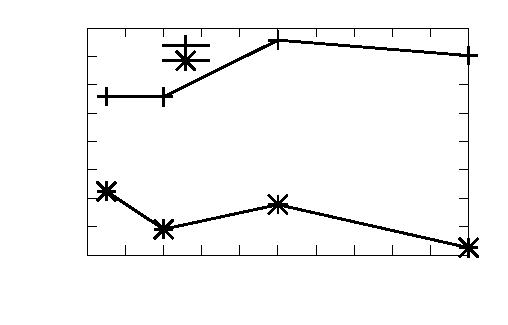
\includegraphics{grass/etc-p1-lin/time.fig.eps}%
\end{picture}%
\setlength{\unitlength}{3947sp}%
%
\begingroup\makeatletter\ifx\SetFigFont\undefined%
\gdef\SetFigFont#1#2#3#4#5{%
  \reset@font\fontsize{#1}{#2pt}%
  \fontfamily{#3}\fontseries{#4}\fontshape{#5}%
  \selectfont}%
\fi\endgroup%
\begin{picture}(3784,2319)(1272,-4012)
\put(1763,-3648){\makebox(0,0)[rb]{\smash{{\SetFigFont{10}{12.0}{\familydefault}{\mddefault}{\updefault} 0.6}}}}
\put(1763,-3421){\makebox(0,0)[rb]{\smash{{\SetFigFont{10}{12.0}{\familydefault}{\mddefault}{\updefault} 0.8}}}}
\put(1763,-3194){\makebox(0,0)[rb]{\smash{{\SetFigFont{10}{12.0}{\familydefault}{\mddefault}{\updefault} 1}}}}
\put(1763,-2967){\makebox(0,0)[rb]{\smash{{\SetFigFont{10}{12.0}{\familydefault}{\mddefault}{\updefault} 1.2}}}}
\put(1763,-2741){\makebox(0,0)[rb]{\smash{{\SetFigFont{10}{12.0}{\familydefault}{\mddefault}{\updefault} 1.4}}}}
\put(1763,-2514){\makebox(0,0)[rb]{\smash{{\SetFigFont{10}{12.0}{\familydefault}{\mddefault}{\updefault} 1.6}}}}
\put(1763,-2287){\makebox(0,0)[rb]{\smash{{\SetFigFont{10}{12.0}{\familydefault}{\mddefault}{\updefault} 1.8}}}}
\put(1763,-2060){\makebox(0,0)[rb]{\smash{{\SetFigFont{10}{12.0}{\familydefault}{\mddefault}{\updefault} 2}}}}
\put(1763,-1833){\makebox(0,0)[rb]{\smash{{\SetFigFont{10}{12.0}{\familydefault}{\mddefault}{\updefault} 2.2}}}}
\put(1838,-3773){\makebox(0,0)[b]{\smash{{\SetFigFont{10}{12.0}{\familydefault}{\mddefault}{\updefault} 0}}}}
\put(2143,-3773){\makebox(0,0)[b]{\smash{{\SetFigFont{10}{12.0}{\familydefault}{\mddefault}{\updefault} 10}}}}
\put(2448,-3773){\makebox(0,0)[b]{\smash{{\SetFigFont{10}{12.0}{\familydefault}{\mddefault}{\updefault} 20}}}}
\put(2753,-3773){\makebox(0,0)[b]{\smash{{\SetFigFont{10}{12.0}{\familydefault}{\mddefault}{\updefault} 30}}}}
\put(3058,-3773){\makebox(0,0)[b]{\smash{{\SetFigFont{10}{12.0}{\familydefault}{\mddefault}{\updefault} 40}}}}
\put(3363,-3773){\makebox(0,0)[b]{\smash{{\SetFigFont{10}{12.0}{\familydefault}{\mddefault}{\updefault} 50}}}}
\put(3668,-3773){\makebox(0,0)[b]{\smash{{\SetFigFont{10}{12.0}{\familydefault}{\mddefault}{\updefault} 60}}}}
\put(3973,-3773){\makebox(0,0)[b]{\smash{{\SetFigFont{10}{12.0}{\familydefault}{\mddefault}{\updefault} 70}}}}
\put(4278,-3773){\makebox(0,0)[b]{\smash{{\SetFigFont{10}{12.0}{\familydefault}{\mddefault}{\updefault} 80}}}}
\put(4583,-3773){\makebox(0,0)[b]{\smash{{\SetFigFont{10}{12.0}{\familydefault}{\mddefault}{\updefault} 90}}}}
\put(4888,-3773){\makebox(0,0)[b]{\smash{{\SetFigFont{10}{12.0}{\familydefault}{\mddefault}{\updefault} 100}}}}
\put(1387,-2679){\rotatebox{90.0}{\makebox(0,0)[b]{\smash{{\SetFigFont{10}{12.0}{\familydefault}{\mddefault}{\updefault}{Processing Time [$sec / MB$] }}}}}}
\put(3363,-3960){\makebox(0,0)[b]{\smash{{\SetFigFont{10}{12.0}{\familydefault}{\mddefault}{\updefault}{Number of Queries}}}}}
\put(2363,-1970){\makebox(0,0)[rb]{\smash{{\SetFigFont{10}{12.0}{\familydefault}{\mddefault}{\updefault}single}}}}
\put(2363,-2095){\makebox(0,0)[rb]{\smash{{\SetFigFont{10}{12.0}{\familydefault}{\mddefault}{\updefault}multi}}}}
\end{picture}%
}
  }
  \caption{Derived products experiment}
\end{figure}

For a different type of derived product, surface albedo was
calculated.  Surface albedo is an important parameter for many
applications.  Albedo is calculated as the minimum pixel value over
some preceding days, here up to the previous 14.  This assumes that at
some point in that time, every pixel in the image had at least one
cloud free acquisition and that clouds are brighter than the surface.
This is a simple calculation, but expensive in that many raster images
need to be accessed to generate the result.
Figure~\ref{fig:albedo_results} shows the comparison between the
single and multi-query optimizations for albedo.  As with the other
derived product, sharing intermediate results leads to increased
processing speed.


\subsection{Multiple Data Products}

The above examples are illustrative, but are not necessarily
representative of a normal set of queries acting on such a system,
since the above queries all request the same data product.  A more
common scenario is where queries are spread among a larger
number of possible data products.  In this case it would be expected
that there is less benefit from the multi-query optimizations, as less
sharing occurs among the queries.

Figures~\ref{fig:medley-lin} and \ref{fig:medley-log} show the results
of a set of queries that access 10 different data products.  The same
query \acp{ROI} were used, but the data products requested were
uniformly distributed among the 5 Imager channels, and 5 other derived
indexes, all normalized ratios.

\begin{figure}[htb]
  \centering
  \subfigure[Fine resolution]{
    \label{fig:medley-lin}
    \scalebox{0.9}{\begin{picture}(0,0)%
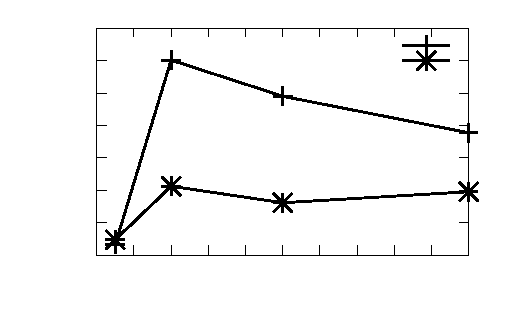
\includegraphics{grass/etc-medley-lin/time.fig.eps}%
\end{picture}%
\setlength{\unitlength}{3947sp}%
%
\begingroup\makeatletter\ifx\SetFigFont\undefined%
\gdef\SetFigFont#1#2#3#4#5{%
  \reset@font\fontsize{#1}{#2pt}%
  \fontfamily{#3}\fontseries{#4}\fontshape{#5}%
  \selectfont}%
\fi\endgroup%
\begin{picture}(3784,2319)(1272,-4012)
\put(1838,-3648){\makebox(0,0)[rb]{\smash{{\SetFigFont{10}{12.0}{\familydefault}{\mddefault}{\updefault} 0.45}}}}
\put(1838,-3389){\makebox(0,0)[rb]{\smash{{\SetFigFont{10}{12.0}{\familydefault}{\mddefault}{\updefault} 0.5}}}}
\put(1838,-3129){\makebox(0,0)[rb]{\smash{{\SetFigFont{10}{12.0}{\familydefault}{\mddefault}{\updefault} 0.55}}}}
\put(1838,-2870){\makebox(0,0)[rb]{\smash{{\SetFigFont{10}{12.0}{\familydefault}{\mddefault}{\updefault} 0.6}}}}
\put(1838,-2611){\makebox(0,0)[rb]{\smash{{\SetFigFont{10}{12.0}{\familydefault}{\mddefault}{\updefault} 0.65}}}}
\put(1838,-2352){\makebox(0,0)[rb]{\smash{{\SetFigFont{10}{12.0}{\familydefault}{\mddefault}{\updefault} 0.7}}}}
\put(1838,-2092){\makebox(0,0)[rb]{\smash{{\SetFigFont{10}{12.0}{\familydefault}{\mddefault}{\updefault} 0.75}}}}
\put(1838,-1833){\makebox(0,0)[rb]{\smash{{\SetFigFont{10}{12.0}{\familydefault}{\mddefault}{\updefault} 0.8}}}}
\put(1913,-3773){\makebox(0,0)[b]{\smash{{\SetFigFont{10}{12.0}{\familydefault}{\mddefault}{\updefault} 0}}}}
\put(2211,-3773){\makebox(0,0)[b]{\smash{{\SetFigFont{10}{12.0}{\familydefault}{\mddefault}{\updefault} 10}}}}
\put(2508,-3773){\makebox(0,0)[b]{\smash{{\SetFigFont{10}{12.0}{\familydefault}{\mddefault}{\updefault} 20}}}}
\put(2806,-3773){\makebox(0,0)[b]{\smash{{\SetFigFont{10}{12.0}{\familydefault}{\mddefault}{\updefault} 30}}}}
\put(3103,-3773){\makebox(0,0)[b]{\smash{{\SetFigFont{10}{12.0}{\familydefault}{\mddefault}{\updefault} 40}}}}
\put(3401,-3773){\makebox(0,0)[b]{\smash{{\SetFigFont{10}{12.0}{\familydefault}{\mddefault}{\updefault} 50}}}}
\put(3698,-3773){\makebox(0,0)[b]{\smash{{\SetFigFont{10}{12.0}{\familydefault}{\mddefault}{\updefault} 60}}}}
\put(3996,-3773){\makebox(0,0)[b]{\smash{{\SetFigFont{10}{12.0}{\familydefault}{\mddefault}{\updefault} 70}}}}
\put(4293,-3773){\makebox(0,0)[b]{\smash{{\SetFigFont{10}{12.0}{\familydefault}{\mddefault}{\updefault} 80}}}}
\put(4591,-3773){\makebox(0,0)[b]{\smash{{\SetFigFont{10}{12.0}{\familydefault}{\mddefault}{\updefault} 90}}}}
\put(4888,-3773){\makebox(0,0)[b]{\smash{{\SetFigFont{10}{12.0}{\familydefault}{\mddefault}{\updefault} 100}}}}
\put(1387,-2679){\rotatebox{90.0}{\makebox(0,0)[b]{\smash{{\SetFigFont{10}{12.0}{\familydefault}{\mddefault}{\updefault}{Processing Time [$sec / MB$] }}}}}}
\put(3400,-3960){\makebox(0,0)[b]{\smash{{\SetFigFont{10}{12.0}{\familydefault}{\mddefault}{\updefault}{Number of Queries}}}}}
\put(4288,-1970){\makebox(0,0)[rb]{\smash{{\SetFigFont{10}{12.0}{\familydefault}{\mddefault}{\updefault}single}}}}
\put(4288,-2095){\makebox(0,0)[rb]{\smash{{\SetFigFont{10}{12.0}{\familydefault}{\mddefault}{\updefault}multi}}}}
\end{picture}%
}
  }
  \subfigure[Coarse resolutions]{
    \label{fig:medley-log}
    \scalebox{0.9}{\begin{picture}(0,0)%
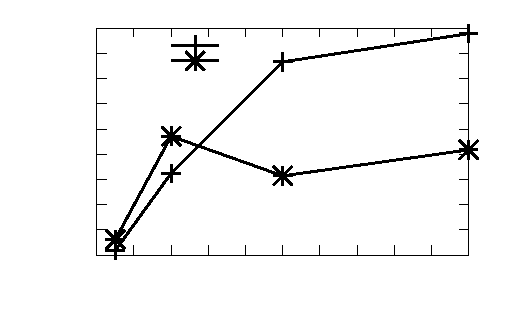
\includegraphics{grass/etc-medley-log/time.fig.eps}%
\end{picture}%
\setlength{\unitlength}{3947sp}%
%
\begingroup\makeatletter\ifx\SetFigFont\undefined%
\gdef\SetFigFont#1#2#3#4#5{%
  \reset@font\fontsize{#1}{#2pt}%
  \fontfamily{#3}\fontseries{#4}\fontshape{#5}%
  \selectfont}%
\fi\endgroup%
\begin{picture}(3784,2319)(1272,-4012)
\put(1838,-3648){\makebox(0,0)[rb]{\smash{{\SetFigFont{10}{12.0}{\familydefault}{\mddefault}{\updefault} 0.3}}}}
\put(1838,-3446){\makebox(0,0)[rb]{\smash{{\SetFigFont{10}{12.0}{\familydefault}{\mddefault}{\updefault} 0.35}}}}
\put(1838,-3245){\makebox(0,0)[rb]{\smash{{\SetFigFont{10}{12.0}{\familydefault}{\mddefault}{\updefault} 0.4}}}}
\put(1838,-3043){\makebox(0,0)[rb]{\smash{{\SetFigFont{10}{12.0}{\familydefault}{\mddefault}{\updefault} 0.45}}}}
\put(1838,-2841){\makebox(0,0)[rb]{\smash{{\SetFigFont{10}{12.0}{\familydefault}{\mddefault}{\updefault} 0.5}}}}
\put(1838,-2640){\makebox(0,0)[rb]{\smash{{\SetFigFont{10}{12.0}{\familydefault}{\mddefault}{\updefault} 0.55}}}}
\put(1838,-2438){\makebox(0,0)[rb]{\smash{{\SetFigFont{10}{12.0}{\familydefault}{\mddefault}{\updefault} 0.6}}}}
\put(1838,-2236){\makebox(0,0)[rb]{\smash{{\SetFigFont{10}{12.0}{\familydefault}{\mddefault}{\updefault} 0.65}}}}
\put(1838,-2035){\makebox(0,0)[rb]{\smash{{\SetFigFont{10}{12.0}{\familydefault}{\mddefault}{\updefault} 0.7}}}}
\put(1838,-1833){\makebox(0,0)[rb]{\smash{{\SetFigFont{10}{12.0}{\familydefault}{\mddefault}{\updefault} 0.75}}}}
\put(1913,-3773){\makebox(0,0)[b]{\smash{{\SetFigFont{10}{12.0}{\familydefault}{\mddefault}{\updefault} 0}}}}
\put(2211,-3773){\makebox(0,0)[b]{\smash{{\SetFigFont{10}{12.0}{\familydefault}{\mddefault}{\updefault} 10}}}}
\put(2508,-3773){\makebox(0,0)[b]{\smash{{\SetFigFont{10}{12.0}{\familydefault}{\mddefault}{\updefault} 20}}}}
\put(2806,-3773){\makebox(0,0)[b]{\smash{{\SetFigFont{10}{12.0}{\familydefault}{\mddefault}{\updefault} 30}}}}
\put(3103,-3773){\makebox(0,0)[b]{\smash{{\SetFigFont{10}{12.0}{\familydefault}{\mddefault}{\updefault} 40}}}}
\put(3401,-3773){\makebox(0,0)[b]{\smash{{\SetFigFont{10}{12.0}{\familydefault}{\mddefault}{\updefault} 50}}}}
\put(3698,-3773){\makebox(0,0)[b]{\smash{{\SetFigFont{10}{12.0}{\familydefault}{\mddefault}{\updefault} 60}}}}
\put(3996,-3773){\makebox(0,0)[b]{\smash{{\SetFigFont{10}{12.0}{\familydefault}{\mddefault}{\updefault} 70}}}}
\put(4293,-3773){\makebox(0,0)[b]{\smash{{\SetFigFont{10}{12.0}{\familydefault}{\mddefault}{\updefault} 80}}}}
\put(4591,-3773){\makebox(0,0)[b]{\smash{{\SetFigFont{10}{12.0}{\familydefault}{\mddefault}{\updefault} 90}}}}
\put(4888,-3773){\makebox(0,0)[b]{\smash{{\SetFigFont{10}{12.0}{\familydefault}{\mddefault}{\updefault} 100}}}}
\put(1387,-2679){\rotatebox{90.0}{\makebox(0,0)[b]{\smash{{\SetFigFont{10}{12.0}{\familydefault}{\mddefault}{\updefault}{Processing Time [$sec / MB$] }}}}}}
\put(3400,-3960){\makebox(0,0)[b]{\smash{{\SetFigFont{10}{12.0}{\familydefault}{\mddefault}{\updefault}{Number of Queries}}}}}
\put(2438,-1970){\makebox(0,0)[rb]{\smash{{\SetFigFont{10}{12.0}{\familydefault}{\mddefault}{\updefault}single}}}}
\put(2438,-2095){\makebox(0,0)[rb]{\smash{{\SetFigFont{10}{12.0}{\familydefault}{\mddefault}{\updefault}multi}}}}
\end{picture}%
}
  }
  \caption{Queries on a 10 data products}
\end{figure}

In this experiment the non-optimized solution performs much closer to
the optimized version.  Besides the fact that there is less chance for
sharing among queries, another fact somewhat idiosyncratic to the
\ac{GOES} data is contributing.  The non-visible channels of the
\ac{GOES} Imager have about a 4 times coarser resolution as compared
to the visible channel.  The previous experiments used the visible
channel as it is the most popular channel, but this example spread
most queries to the other channels, less averaging was required by
each query.  This further reduces the opportunities for queries to
share intermediate data.


\subsection{Reducing Secondary Storage Costs}

Some of the tradeoffs between using existing \ac{GIS} applications
versus developing specific applications for streaming \ac{RSI} data
were discussed previously.  Chief among considerations was the added
cost of secondary I/O usage.  One method of minimizing I/O costs while
allowing traditional applications like \ac{GRASS} would be to use a
large RAM filesystem for processing images.  The current system does
not include enough free RAM to perform the experiments described
above.  However, some preliminary experiments were undertaken.
Specifically, the \ac{GRASS} database of \ac{GOES} data was copied to
a RAM filesystem.  A 5 query, multiple data product experiment was run
with all intermediate and result data products produced on the RAM
filesystem.  Comparison of these times to the previously reported
show only a moderate, ~10\% decrease in the overall processing time
for the RAM filesystem.  While this is not necessarily an indicator of
expected speeds for a specially crafted \ac{DSMS}, it does indicate
that other aspects of the workflow processing besides I/O affect
system performance.

% A considerable 

% \begin{table}
%   \centering
%   \caption{Experiment sizes}
%   \begin{tabular}{l|c|c|c|c|c|c}
%     Experiment & \multicolumn{2}{|c|}{Total Size \unit[GB]} \\
%       & Each & Share & \unit[GB] \\
%       \hline \hline
%       Restriction, Fine & 7.5   & 4.9  & 2.4 \\
%       Restriction, Coarse & 7.6 & 4.4  & 2.2 \\
%       Derived, Fine& 10.0 & 5.0 & 2.4 \\
%       Medley, Fine &  5.5 & 5.0  & 1.9 \\
%       Medley, Coarse & 5.4 & 4.4  & 1.9 \\
%   \end{tabular}
%   \label{tab:exp}
% \end{table}


\section{Discussion}
\label{sec:gis-conclusions}

For large numbers of continuous queries against \ac{RSI}, optimization
over multiple queries has been shown to be an effective method of
increasing the overall system performance.  How much savings can be
expected depends primarily on the relationships among the queries in
the system.

The optimization strategy optimizes individual queries first and then
combines these using the methodology for building a \ac{QEG}
described in Section~\ref{sec:multi}.  Operators are reused for
multiple queries with spatial restrictions modified to encompass all
appropriate query \acp{ROI}.

The implementation uses existing \ac{GRASS} \ac{GIS} applications, to
execute the processing steps.  Remotely sensed imagery clearly
provides a great opportunity to study concepts and paradigms for the
management and processing of streaming data, given the existence of
various satellites that are used constantly for numerous data
products.  Even if new processing methods are developed for processing
these images operations on a finer scale--for example processing rows
of data at a time as described in Chapter~\ref{cha:operators}--the
experiments presented here inform the developer on predicted levels of
data sharing that will exist in such a system.

The ideas presented here are described in terms of continuous queries
over \ac{RSI}; however similar opportunities exist in other applications and
incoming data streams.  Another good candidates include model outputs.
For example, the \ac{WRF} model, can be run in modes that periodically
output weather predictions.

\section{Related Work}
\label{sec:related-gis}

The results showing performance increases with optimizations in an
existing \ac{GIS} application were first described by
Hart~\cite{hart06optim-of}.  Previous studies have recognized the
critical role played by many data producers manipulating and making
available \ac{RSI} products to support environmental applications.
One example, the Earth Science
Workbench~\cite{DBLP:conf/ssdbm/FrewB01}, describes a system for
developing standardized workflows on locally received satellite image
data that is very similar in context to individual user queries here.
Similarly, the Goddard Earth Sciences Data and Information Services
Center is developing a service of virtual data products that
reproduce the data from original sources dynamically based on the
queries to the system~\cite{DBLP:conf/ssdbm/LynnesV05}.

None of the above systems looked at combining multiple image
processing workflows into a more efficient computation strategies.
This is in part because the focus of these efforts centered on
traditional historical queries.


\chapter{The Dynamic Cascade Tree}
\label{cha:dct}

The multi-query optimization techniques developed previously require
an operator that is able to provide restrictions for multiple query
\ac{ROI}.  \ac{RSI} row tuples enter the operator at high data rates,
and there can be many individual \acp{ROI} handled by the system.
Later, in Chapter~\ref{cha:operators} operators for an on-line
\ac{DSMS} will be discussed.  The implementation of the spatial
transformation operator will require a similar restriction operator
with very many \acp{ROI}, a individual \ac{ROI} for each row in the
output point lattice coordinate system.  

In this chapter, query processing for image restrictions on streaming
\ac{RSI} data is investigated.  The approach uses a \acf{DCT} to index
spatio-temporal query \acp{ROI} and to efficiently determine what
incoming \ac{RSI} data is relevant to what queries.  The \ac{DCT}
exploits spatial trends in incoming \ac{RSI} data to efficiently
filter the data that is of interest to the individual query \ac{ROI}.
Experimental results using random input and \acf{GOES} data give a
good insight into processing streaming \ac{RSI} and verify the
efficiency and utility of the \ac{DCT}.

Most continuous queries against an \acs{RSI} data stream include
operations to restrict the spatio-temporal data to specified
\acp{ROI}.  Such \emph{\acf{CQ} \ac{ROI}} are part of more complex
queries users issue against a \acs{DSMS}.  Clearly, query \acp{ROI}
specified by different users may overlap.  This is typical for
\ac{RSI} streams which have geographic \emph{hot spots} or regions
that are of interest to many users.  An \acs{RSI} stream management
system needs to (1) efficiently intersect incoming image data with a
possibly large number of query \acp{ROI}, and (2) it should provide a
means that allows queries to share the incoming data for further
processing. These aspects are illustrated in
Figure~\ref{fig:query-eval2} where one \ac{ROI} $R_i$ is
associated with each of the user queries $Q_i$.  In the figure,
incoming \acs{RSI} data intersects with two query \acp{ROI} $R_1$ and
$R_2$ (left). Instead of filtering incoming data for each individual
query $Q_1, Q_2$, and $Q_3$ (middle), a mechanism is needed to
determine what incoming image data is relevant to what queries and
pipelines the relevant data to subsequent query operators.  The
\acs{DCT} is such a mechanism, which filters and streams relevant data
to subsequent operators of individual queries, here only $Q_1'$ and
$Q_2'$ (right).  In efficiently processing these spatial restrictions,
the organization of the incoming data stream needs to be considered.

\begin{figure}[htb]
  \centering
  \scalebox{1.5}{\begin{picture}(0,0)%
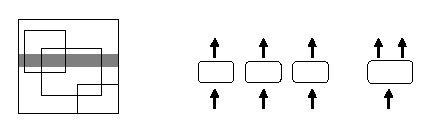
\includegraphics{figs/query-eval.fig.eps}%
\end{picture}%
\setlength{\unitlength}{4144sp}%
%
\begingroup\makeatletter\ifx\SetFigFont\undefined%
\gdef\SetFigFont#1#2#3#4#5{%
  \reset@font\fontsize{#1}{#2pt}%
  \fontfamily{#3}\fontseries{#4}\fontshape{#5}%
  \selectfont}%
\fi\endgroup%
\begin{picture}(3030,792)(-11,59)
\put(2686,419){\makebox(0,0)[lb]{\smash{{\SetFigFont{5}{6.0}{\familydefault}{\mddefault}{\updefault}{\color[rgb]{0,0,0}\dct}%
}}}}
\put( 91,659){\makebox(0,0)[lb]{\smash{{\SetFigFont{5}{6.0}{\familydefault}{\mddefault}{\updefault}{\color[rgb]{0,0,0}$R_1$}%
}}}}
\put(226,299){\makebox(0,0)[lb]{\smash{{\SetFigFont{5}{6.0}{\familydefault}{\mddefault}{\updefault}{\color[rgb]{0,0,0}$R_2$}%
}}}}
\put(496,164){\makebox(0,0)[lb]{\smash{{\SetFigFont{5}{6.0}{\familydefault}{\mddefault}{\updefault}{\color[rgb]{0,0,0}$R_3$}%
}}}}
\put(811,479){\makebox(0,0)[lb]{\smash{{\SetFigFont{5}{6.0}{\familydefault}{\mddefault}{\updefault}{\color[rgb]{0,0,0}RSI}%
}}}}
\put(1416,738){\makebox(0,0)[lb]{\smash{{\SetFigFont{5}{6.0}{\familydefault}{\mddefault}{\updefault}{\color[rgb]{0,0,0}$Q_1$}%
}}}}
\put(1787,738){\makebox(0,0)[lb]{\smash{{\SetFigFont{5}{6.0}{\familydefault}{\mddefault}{\updefault}{\color[rgb]{0,0,0}$Q_2$}%
}}}}
\put(2157,738){\makebox(0,0)[lb]{\smash{{\SetFigFont{5}{6.0}{\familydefault}{\mddefault}{\updefault}{\color[rgb]{0,0,0}$Q_3$}%
}}}}
\put(1388,404){\makebox(0,0)[lb]{\smash{{\SetFigFont{5}{6.0}{\familydefault}{\mddefault}{\updefault}{\color[rgb]{0,0,0}$R_1$}%
}}}}
\put(1748,404){\makebox(0,0)[lb]{\smash{{\SetFigFont{5}{6.0}{\familydefault}{\mddefault}{\updefault}{\color[rgb]{0,0,0}$R_2$}%
}}}}
\put(2108,404){\makebox(0,0)[lb]{\smash{{\SetFigFont{5}{6.0}{\familydefault}{\mddefault}{\updefault}{\color[rgb]{0,0,0}$R_3$}%
}}}}
\put(1441, 74){\makebox(0,0)[lb]{\smash{{\SetFigFont{5}{6.0}{\familydefault}{\mddefault}{\updefault}{\color[rgb]{0,0,0}RSI}%
}}}}
\put(1801, 74){\makebox(0,0)[lb]{\smash{{\SetFigFont{5}{6.0}{\familydefault}{\mddefault}{\updefault}{\color[rgb]{0,0,0}RSI}%
}}}}
\put(2161, 74){\makebox(0,0)[lb]{\smash{{\SetFigFont{5}{6.0}{\familydefault}{\mddefault}{\updefault}{\color[rgb]{0,0,0}RSI}%
}}}}
\put(2746, 74){\makebox(0,0)[lb]{\smash{{\SetFigFont{5}{6.0}{\familydefault}{\mddefault}{\updefault}{\color[rgb]{0,0,0}RSI}%
}}}}
\put(2656,749){\makebox(0,0)[lb]{\smash{{\SetFigFont{5}{6.0}{\familydefault}{\mddefault}{\updefault}{\color[rgb]{0,0,0}$Q_1'$}%
}}}}
\put(2836,749){\makebox(0,0)[lb]{\smash{{\SetFigFont{5}{6.0}{\familydefault}{\mddefault}{\updefault}{\color[rgb]{0,0,0}$Q_2'$}%
}}}}
\end{picture}%
  }
  \caption{Restriction operation on multiple queries} 
\label{fig:query-eval2}
\end{figure}

Section~\ref{sec:dm} describes how \ac{RSI} data is transmitted from
the instrument and shows an important characteristic exploited in the
following approach.  Consecutive packets in a stream of \ac{RSI} data
have close spatial and temporal proximity, though there are some
exceptions, for example, where the last pixel of a line in an image is
followed by the first pixel of a new image.  In the \ac{DCT}, this
spatial trend is used to influence on how multiple queries against a
stream of \ac{RSI} data are processed.

The \acf{DCT} is a space efficient structure to index query \acp{ROI}
that are part of more complex queries against \acs{RSI} data streams.
The concepts underlying the \acs{DCT} are introduced using an incoming
stream of points.  The problem generalizes to solving many
\emph{stabbing point} queries.  The \ac{DCT} is then extended to consider
rectangular extents from streaming \ac{RSI} data.  The \acs{DCT}
supports the efficient processing of a \emph{moving data stream}.  A
data stream query is one that, for a window describing the spatial
extent of incoming image data (pixel, row, or image), will identify
all \ac{CQ} \acp{ROI} that spatially and temporally overlap the data
window. This not only allows the pipelining of image data to those
queries to which the data is of interest, but it also facilitates the
sharing of image data among queries in the case of non-disjoint query
regions. The design of the data structures and algorithms underlying
the \acs{DCT} are guided by the some important requirements, which are
typical for \acs{RSI} data streams:

\begin{itemize}
\item The \acs{DCT} indexes \ac{CQ} \acp{ROI} and is
  sufficiently small to be kept in main memory. It also has to support
  efficient insertion and deletion of \ac{CQ} \acp{ROI}.
  
\item The geospatial data stream comes from a single source
  corresponding to the real-time incoming streaming satellite data.
  Sequential stream data is usually in close proximity and have a
  regular trajectory through space. The \acs{DCT} has to account for
  both the size and the spatio-temporal trends of the incoming data
  stream.
  
\item Because of the size of the \ac{CQ} \acp{ROI} and the
  size and shape of the data in the input stream, selectivity is high.
  For example, incoming \ac{RSI} data stream packets intersect about
  \%20 of \ac{CQ} \acp{ROI} for typical \acs{GOES} applications.
\end{itemize}

Section~\ref{sec:dct-point} introduces a simplified version of the
\ac{DCT} for incoming point queries.  Section~\ref{sec:dct-win}
describes the \acs{DCT} for window queries and shows how it filters
incoming image data streams for multiple \ac{CQ} \acp{ROI}.
Section~\ref{sec:performance} discusses the performance of the
\acs{DCT} in general terms and discusses the parameters affecting
performance.  In Section~\ref{sec:experiments}, several experimental
results are presented.  These include experiments on random data to
study the performance under changing input parameters, and experiments
closer to real world scenarios using \ac{GOES} input data as an
example.  Section \ref{sec:temporal} explores adding a temporal
dimension to the \acs{DCT}.  Section~\ref{sec:related} describes
related research for similar problem domains.

\section{\ac{DCT} for Point Queries}
\label{sec:dct-point}

The problem of quickly answering multiple queries on a stream of RSI
data is basically solving a normal \emph{stabbing
  query}~\cite{berg00comput-geomet} for a point. That is, as query
result, a stabbing query determines all query \acp{ROI} that contain the
current point delivered by the RSI data stream.
For \ac{RSI} data, the stabbing points are special in that the next
stabbing point is typically very close to the previous stabbing point.
The goal is to take advantage of the trendiness of stabbing points and
to develop index structures that improve the search performance for
subsequent stabbing queries.

The structure proposed in the following builds an index that is
dynamically tuned to the current location of RSI data.  For a given
point, the \ac{DCT} maintains the regions around that point where the
query result will change.  Stabbing queries can be answered in
constant time if the new stabbing point has the same result as the
previous query and will incrementally update a new result set based on
the previous set when the result is different.  The structure is
designed to be small and quickly allow for insertions and deletions of
new query \acp{ROI}.  It assumes some particular characteristics of the
input stream, notably that the stream changes in such a way that many
subsequent incoming \acs{RSI} data will contribute to the same result
set(s) to region queries as the current point. Therefore, the cost of
maintaining a dynamic structure can be amortized over a large set of
queries.

\subsection{\ac{DCT} Components}

Figure~\ref{fig:cascade-tree} gives an overview of the \ac{DCT} data
structure.  The figure shows a set of query \acp{ROI} $a, b, \ldots,
f$, the node, \id{cn}, corresponding to the most recent stabbing point
from the data stream, and the associated structures for the \ac{DCT}.
The figure describes a \ac{DCT} that indexes two dimensions.  There
is no required order in how the dimensions are referenced, and the
example shows the vertical ($y$) dimension being the first dimension
indexed in the \ac{DCT}.

\begin{figure}[htb]
  \centering
  \begin{picture}(0,0)%
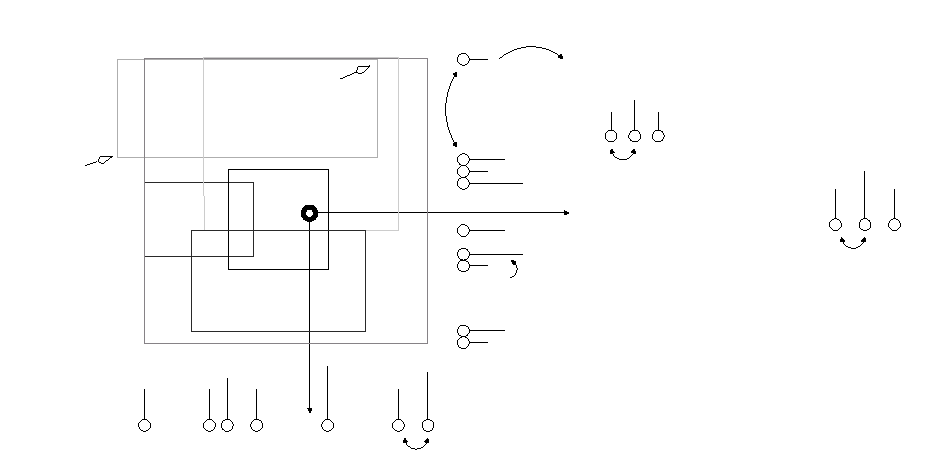
\includegraphics{figs/dct-point.fig.eps}%
\end{picture}%
\setlength{\unitlength}{4144sp}%
%
\begingroup\makeatletter\ifx\SetFigFontNFSS\undefined%
\gdef\SetFigFontNFSS#1#2#3#4#5{%
  \reset@font\fontsize{#1}{#2pt}%
  \fontfamily{#3}\fontseries{#4}\fontshape{#5}%
  \selectfont}%
\fi\endgroup%
\begin{picture}(6887,3294)(421,-3175)
\put(3781,-556){\makebox(0,0)[lb]{\smash{{\SetFigFontNFSS{8}{9.6}{\familydefault}{\mddefault}{\updefault}{\color[rgb]{0,0,0}Nodes are}%
}}}}
\put(3781,-691){\makebox(0,0)[lb]{\smash{{\SetFigFontNFSS{8}{9.6}{\familydefault}{\mddefault}{\updefault}{\color[rgb]{0,0,0}linked}%
}}}}
\put(3826,-2131){\makebox(0,0)[lb]{\smash{{\SetFigFontNFSS{8}{9.6}{\familydefault}{\mddefault}{\updefault}{\color[rgb]{0,0,0}searchable}%
}}}}
\put(3826,-1996){\makebox(0,0)[lb]{\smash{{\SetFigFontNFSS{8}{9.6}{\familydefault}{\mddefault}{\updefault}{\color[rgb]{0,0,0}Lists are}%
}}}}
\put(5041,-736){\makebox(0,0)[lb]{\smash{{\SetFigFontNFSS{8}{9.6}{\rmdefault}{\mddefault}{\updefault}{\color[rgb]{0,0,0}b}%
}}}}
\put(5221,-736){\makebox(0,0)[lb]{\smash{{\SetFigFontNFSS{8}{9.6}{\rmdefault}{\mddefault}{\updefault}{\color[rgb]{0,0,0}c}%
}}}}
\put(4861,-736){\makebox(0,0)[lb]{\smash{{\SetFigFontNFSS{8}{9.6}{\rmdefault}{\mddefault}{\updefault}{\color[rgb]{0,0,0}a}%
}}}}
\put(4051,-2761){\makebox(0,0)[lb]{\smash{{\SetFigFontNFSS{8}{9.6}{\familydefault}{\mddefault}{\updefault}{\color[rgb]{0,0,0}$L_2$ only contains regions}%
}}}}
\put(4051,-2896){\makebox(0,0)[lb]{\smash{{\SetFigFontNFSS{8}{9.6}{\familydefault}{\mddefault}{\updefault}{\color[rgb]{0,0,0}whose $y$ domain }%
}}}}
\put(4051,-3031){\makebox(0,0)[lb]{\smash{{\SetFigFontNFSS{8}{9.6}{\familydefault}{\mddefault}{\updefault}{\color[rgb]{0,0,0}includes current point}%
}}}}
\put(2161,-2896){\makebox(0,0)[lb]{\smash{{\SetFigFontNFSS{8}{9.6}{\rmdefault}{\mddefault}{\updefault}{\color[rgb]{0,0,0}d}%
}}}}
\put(4726,-376){\makebox(0,0)[lb]{\smash{{\SetFigFontNFSS{8}{9.6}{\familydefault}{\mddefault}{\updefault}{\color[rgb]{0,0,0}has set of regions}%
}}}}
\put(4726,-241){\makebox(0,0)[lb]{\smash{{\SetFigFontNFSS{8}{9.6}{\familydefault}{\mddefault}{\updefault}{\color[rgb]{0,0,0}Each node in $L_2$}%
}}}}
\put(5986,-1951){\makebox(0,0)[lb]{\smash{{\SetFigFontNFSS{8}{9.6}{\familydefault}{\mddefault}{\updefault}{\color[rgb]{0,0,0}$A$ contains regions in}%
}}}}
\put(5986,-2086){\makebox(0,0)[lb]{\smash{{\SetFigFontNFSS{8}{9.6}{\familydefault}{\mddefault}{\updefault}{\color[rgb]{0,0,0}$L_2$ whose $x$ domain}%
}}}}
\put(5986,-2221){\makebox(0,0)[lb]{\smash{{\SetFigFontNFSS{8}{9.6}{\familydefault}{\mddefault}{\updefault}{\color[rgb]{0,0,0}includes current point}%
}}}}
\put(3826,-16){\makebox(0,0)[lb]{\smash{{\SetFigFontNFSS{10}{12.0}{\familydefault}{\mddefault}{\updefault}{\color[rgb]{0,0,0}$L_1$}%
}}}}
\put(1216,-286){\makebox(0,0)[lb]{\smash{{\SetFigFontNFSS{8}{9.6}{\rmdefault}{\mddefault}{\updefault}{\color[rgb]{0,0,0}a}%
}}}}
\put(1441,-286){\makebox(0,0)[lb]{\smash{{\SetFigFontNFSS{8}{9.6}{\rmdefault}{\mddefault}{\updefault}{\color[rgb]{0,0,0}b}%
}}}}
\put(1891,-286){\makebox(0,0)[lb]{\smash{{\SetFigFontNFSS{8}{9.6}{\rmdefault}{\mddefault}{\updefault}{\color[rgb]{0,0,0}c}%
}}}}
\put(2701,-1141){\makebox(0,0)[lb]{\smash{{\SetFigFontNFSS{8}{9.6}{\rmdefault}{\mddefault}{\updefault}{\color[rgb]{0,0,0}e}%
}}}}
\put(1801,-2221){\makebox(0,0)[lb]{\smash{{\SetFigFontNFSS{8}{9.6}{\rmdefault}{\mddefault}{\updefault}{\color[rgb]{0,0,0}f}%
}}}}
\put(4726,-1411){\makebox(0,0)[lb]{\smash{{\SetFigFontNFSS{8}{9.6}{\familydefault}{\mddefault}{\updefault}{\color[rgb]{0,0,0}denote location}%
}}}}
\put(1441,-2896){\makebox(0,0)[lb]{\smash{{\SetFigFontNFSS{8}{9.6}{\rmdefault}{\mddefault}{\updefault}{\color[rgb]{0,0,0}b,d}%
}}}}
\put(1936,-2896){\makebox(0,0)[lb]{\smash{{\SetFigFontNFSS{8}{9.6}{\rmdefault}{\mddefault}{\updefault}{\color[rgb]{0,0,0}e}%
}}}}
\put(2701,-2896){\makebox(0,0)[lb]{\smash{{\SetFigFontNFSS{8}{9.6}{\rmdefault}{\mddefault}{\updefault}{\color[rgb]{0,0,0}e}%
}}}}
\put(3241,-2896){\makebox(0,0)[lb]{\smash{{\SetFigFontNFSS{8}{9.6}{\rmdefault}{\mddefault}{\updefault}{\color[rgb]{0,0,0}c}%
}}}}
\put(3466,-2896){\makebox(0,0)[lb]{\smash{{\SetFigFontNFSS{8}{9.6}{\rmdefault}{\mddefault}{\updefault}{\color[rgb]{0,0,0}b}%
}}}}
\put(1801,-2896){\makebox(0,0)[lb]{\smash{{\SetFigFontNFSS{8}{9.6}{\rmdefault}{\mddefault}{\updefault}{\color[rgb]{0,0,0}c}%
}}}}
\put(6571,-1411){\makebox(0,0)[lb]{\smash{{\SetFigFontNFSS{8}{9.6}{\rmdefault}{\mddefault}{\updefault}{\color[rgb]{0,0,0}b}%
}}}}
\put(7021,-1411){\makebox(0,0)[lb]{\smash{{\SetFigFontNFSS{8}{9.6}{\rmdefault}{\mddefault}{\updefault}{\color[rgb]{0,0,0}e}%
}}}}
\put(6796,-1411){\makebox(0,0)[lb]{\smash{{\SetFigFontNFSS{8}{9.6}{\rmdefault}{\mddefault}{\updefault}{\color[rgb]{0,0,0}c}%
}}}}
\put(1411,-1238){\makebox(0,0)[lb]{\smash{{\SetFigFontNFSS{8}{9.6}{\rmdefault}{\mddefault}{\updefault}{\color[rgb]{0,0,0}d}%
}}}}
\put(436,-429){\makebox(0,0)[lb]{\smash{{\SetFigFontNFSS{8}{9.6}{\familydefault}{\mddefault}{\updefault}{\color[rgb]{0,0,0}with $r_{id} = a$}%
}}}}
\put(436,-294){\makebox(0,0)[lb]{\smash{{\SetFigFontNFSS{8}{9.6}{\familydefault}{\mddefault}{\updefault}{\color[rgb]{0,0,0}region $r$ }%
}}}}
\put(4726,-1546){\makebox(0,0)[lb]{\smash{{\SetFigFontNFSS{8}{9.6}{\familydefault}{\mddefault}{\updefault}{\color[rgb]{0,0,0}of current node}%
}}}}
\put(5986,-1411){\makebox(0,0)[lb]{\smash{{\SetFigFontNFSS{10}{12.0}{\familydefault}{\mddefault}{\updefault}{\color[rgb]{0,0,0}$A$}%
}}}}
\put(4726,-1276){\makebox(0,0)[lb]{\smash{{\SetFigFontNFSS{8}{9.6}{\familydefault}{\mddefault}{\updefault}{\color[rgb]{0,0,0}$cn_1, cn_2$}%
}}}}
\put(901,-2896){\makebox(0,0)[lb]{\smash{{\SetFigFontNFSS{10}{12.0}{\familydefault}{\mddefault}{\updefault}{\color[rgb]{0,0,0}$L_2$}%
}}}}
\put(586,-1141){\makebox(0,0)[lb]{\smash{{\SetFigFontNFSS{8}{9.6}{\familydefault}{\mddefault}{\updefault}{\color[rgb]{0,0,0}$(\ryn,\rxn)$}%
}}}}
\put(2656,-466){\makebox(0,0)[lb]{\smash{{\SetFigFontNFSS{8}{9.6}{\familydefault}{\mddefault}{\updefault}{\color[rgb]{0,0,0}(\ryx,\rxx)}%
}}}}
\end{picture}%

  \caption[\acf{DCT}]{\acf{DCT} with query \acp{ROI} $a,b, \ldots, f$;
    A query \ac{ROI}, \r, is described by minimum (lower left) corner
    $(\ryn, \rxn)$ and maximum (upper right) corner $(\ryx,
    \rxx)$}
  \label{fig:cascade-tree}
\end{figure}

The components of \ac{DCT} are pleasantly simple extensions to a
binary tree.  In the example and following pseudo-code, there are two
simple search structures, \id{List} and \id{2KeyList}.  \id{List}
supports \func{Insert}{key,value}, \func{Delete}{key}, and
\func{Enumerate}{}.  Keys in \id{List} are unique for each value.  One
implementation could use a simple skip list~\cite{pugh90skip} to
implement \id{List}.  

The \id{2KeyList} is incrementally more complex.  It supports
\func{Insert}{\id{key_1}, \id{key_2}, \id{value}},
\func{Delete}{\id{key_1}, \id{key_2}} and \func{Enumerate}{\id{key_1}}
using two keys.  The combination of two keys is unique for each value.
\func{Enumerate}{\id{key_1}} enumerates all the values in the
\id{2KeyList}, entered with \id{key_1}.  An implementation of
\id{2KeyList} could be a skip list using \id{key_1}, where each node
has an associated skip list using \id{key_2}.  With this
implementation, for $\id{2KeyList}
\METH{delete}{\id{key_1},\id{key_2}}$, if the deletion causes an empty
set in the associated \id{key_1} node, then that entire node is
deleted.

\id{List} leaf nodes contain \ac{ROI} ids, \rid\ as keys with a pointer to
the query \ac{ROI}, \r\ as the value.  For the \id{2KeyList}, \id{key_1} is the
value of the endpoint, and \id{key_2} is the identifier of the query
\ac{ROI}, denoted \rid.  The leaf nodes of a \id{2KeyList} correspond to the
half-open line segments.  Leaf nodes of a \id{2KeyList} also have pointers
to the next and previous nodes in sorted order, allowing for linked
list traversal to the leaf nodes.  One reason for choosing a skip list
implementation is that the forward pointers already exist, and only an
additional back pointer is added to a normal skip list.

The \ac{DCT} maintains a separate \id{2KeyList} for each dimension of the
individual query \acp{ROI}.  In the example of Figure~\ref{fig:cascade-tree},
these are \id{L_1} and \id{L_2}.  In addition, the \ac{DCT} maintains a \id{List}, \id{A}, of
all query \acp{ROI}, which overlap the current stabbing point.  A second
structure, \id{cn}, maintains pointers to nodes within each \id{2KeyList},
corresponding to the most current stabbing point.

The \id{2KeyList} for the first dimension, \id{L_1} contains the minimum and
maximum endpoints in the 1st ($y$) dimension, $(\ryn,\ryx)$, for
every query \ac{ROI} \r.

The next \id{2KeyList}, \id{L_2} contains keys on the endpoints in the 2nd ($x$)
dimension and \rid.  \id{L_2} does not contain the endpoints of all the
\acp{ROI} in \ac{DCT}, but only the \acp{ROI} whose 1st dimension ($y$)
overlap with the current node, \id{cn_1}.

If the query \acp{ROI} contained more dimensions, additional \id{2KeyList} 
structures would be added to the \ac{DCT}, where each subsequent \id{2KeyList} 
only indexes those \acp{ROI} that overlap the current point up to that
dimension.

In Figure~\ref{fig:cascade-tree}, \id{cn} contains two pointers, \id{cn_1} and
\id{cn_2} to nodes within both \id{L_1} and \id{L_2} corresponding to the location
of the most recent stabbing point.

\id{A} is the final \id{List} that contains all the currently selected query
\acp{ROI} that correspond to the current stabbing point query.  Just as
\id{L_2} contains only a subset of the \acp{ROI} of \id{L_1} that contain the
\id{cn_1} node, \id{A} contains the subset of \id{L_2} where the \id{cn_2} node is
contained by the 2nd dimension of each \ac{ROI}.  The \id{L_1}, \id{L_2}, and \id{A} 
structures make up a cascade of indexes, each a subset of the previous
index.

\subsection{Updating Query \acp{ROI}}

The \ac{DCT} is initialized by creating the \id{2KeyList} and
\id{List} structures, adding a starting node for \id{L_2} and \id{L_1}
outside their valid range, and assigning \id{cn_2} and \id{cn_1} to
those nodes.

Algorithm~\ref{alg:insert} shows the pseudo-code for inserting query
\acp{ROI} into \ac{DCT}.  Insertion and deletion are simple
routines. For insertion, a \ac{ROI} is first inserted into \id{L_1},
and then successively into \id{L_2} and \id{A} if the \ac{ROI}
overlaps the current node, \id{cn} in the other dimensions.
\proc{Delete-Region} is similar to the insertion, taking the \ac{ROI}
\r\ as input.

\begin{pseudocode}[ruled]{Insert-Region}{\ac{DCT},\id{cn},\r}
\label{alg:insert}
\PROCEDURE{Insert-Ith}{\ac{DCT},\id{cn},\r,i}
%\COMMENT{Input: \ac{DCT},\id{cn},\r\ same as \CALL{Insert-Region}{}}\\
%\COMMENT{\phantom{Input:} dimension, $i$}\\
  I \GETS \id{L_i} \hfill \COMMENT{$i$th \id{2KeyList}}\\
  \IF (i > \text{ dimensions of } r) 
  \THEN \id{A} \METH{insert}{\rid,\r}
  \ELSE 
  \BEGIN
    I \METH{insert}{\rin,\rid,\r}\\
    I \METH{insert}{\rix,\rid,\r}\\
    \IF (\rin \leq \id{cn_i} .key \text{ and } \rix > \id{cn_i} .key)
      \THEN \CALL{Insert-Ith}{\ac{DCT},\id{cn},\r,i+1}
  \END
\ENDPROCEDURE
\MAIN
%\COMMENT{Input: \ac{DCT},}\\
%\COMMENT{\phantom{Input:} current node \id{cn} = \{\id{cn_2},\id{cn_1}}}\\
%\COMMENT{\phantom{Input:} \ac{ROI}, $\r = \{\rxn,\ryn,\rxx,\ryx\}$}\\
\CALL{Insert-Ith}{\ac{DCT},\id{cn},\r,1}
\ENDMAIN
\end{pseudocode}
   
The structures \id{L_2} and \id{A} need to be maintained when new
\acp{ROI} are inserted and deleted, and for each new stabbing point.
Since \id{L_2} contains \acp{ROI} overlapping the current node,
\id{cn}, when a new stabbing point arrives where a $y$ boundary for
any \ac{ROI} in the \ac{DCT} is crossed, then the \id{L_2} structure
needs to be modified to account for the \acp{ROI} to be included or
deleted from consideration.  A similar method needs to be associated
with boundary crossings in the $x$ dimension while traversing \id{L_2}
and modifying \id{A}.

\subsection{Querying}

The algorithm for reporting selected (active) query \acp{ROI} for a new
stabbing point $\np = (\npy,\npx)$, begins by traversing the \id{2KeyList} 
\id{L_1} in the $y$ direction from the current node $cn=(cn_1,cn_2)$ to
the node containing \npy\ going through every intermediate node using
the linked list access on the leaf nodes of \id{L_1}.  At each boundary
crossing, as \acp{ROI} are entered or exited, those \acp{ROI} need to be
added to or deleted from the \id{L_2} \id{2KeyList}. When the point has traversed
to the node containing \npy, then traversal begins in the $x$
direction, moving from \id{cn_2} to the node containing \npx.  As with \id{L_1},
when the traversal hits $x$ boundary points, then the entered query
\acp{ROI} are added to \id{A} and the exited \acp{ROI} are deleted from \id{A}.
When the traversal reaches $\np$, then \id{cn} contains pointers to the
nodes containing the \np, \id{L_2} contains $x$ endpoints to all the
\acp{ROI} with $y$ domains that contain \npy, and \id{A} lists all \acp{ROI}
that contain \np.  \id{A} is then enumerated to report all the query
\acp{ROI} that are affected by the new stabbing point \np.

\begin{figure}[htb]
%  \centering
  \begin{picture}(0,0)%
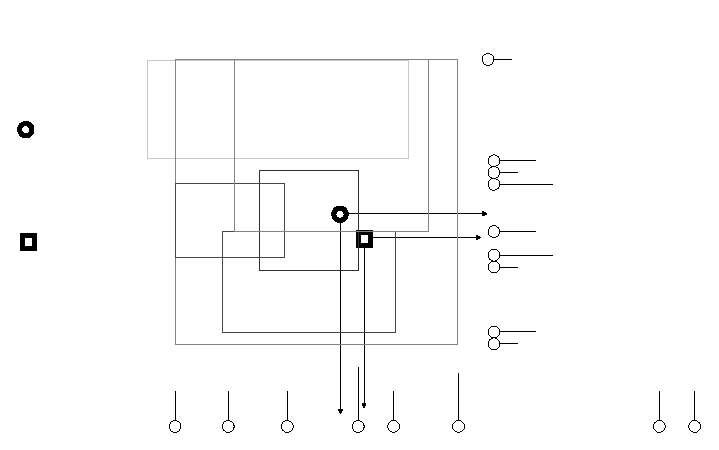
\includegraphics{figs/move-point.fig.eps}%
\end{picture}%
\setlength{\unitlength}{4144sp}%
%
\begingroup\makeatletter\ifx\SetFigFontNFSS\undefined%
\gdef\SetFigFontNFSS#1#2#3#4#5{%
  \reset@font\fontsize{#1}{#2pt}%
  \fontfamily{#3}\fontseries{#4}\fontshape{#5}%
  \selectfont}%
\fi\endgroup%
\begin{picture}(5220,3170)(-404,-2551)
\put(4178,-158){\makebox(0,0)[lb]{\smash{{\SetFigFontNFSS{10}{12.0}{\familydefault}{\mddefault}{\updefault}{\color[rgb]{0,0,0}{\bf 2.} c is removed from $L_2$ and}%
}}}}
\put(4178,-338){\makebox(0,0)[lb]{\smash{{\SetFigFontNFSS{10}{12.0}{\familydefault}{\mddefault}{\updefault}{\color[rgb]{0,0,0}f is inserted into $L_2$}%
}}}}
\put(4178,-1238){\makebox(0,0)[lb]{\smash{{\SetFigFontNFSS{10}{12.0}{\familydefault}{\mddefault}{\updefault}{\color[rgb]{0,0,0}{\bf 4.} c and e are removed from $A$}%
}}}}
\put(4178,-1418){\makebox(0,0)[lb]{\smash{{\SetFigFontNFSS{10}{12.0}{\familydefault}{\mddefault}{\updefault}{\color[rgb]{0,0,0}and f is inserted into $A$}%
}}}}
\put(4178,337){\makebox(0,0)[lb]{\smash{{\SetFigFontNFSS{10}{12.0}{\familydefault}{\mddefault}{\updefault}{\color[rgb]{0,0,0}{\bf 1.} New point $np$ crosses }%
}}}}
\put(4178,157){\makebox(0,0)[lb]{\smash{{\SetFigFontNFSS{10}{12.0}{\familydefault}{\mddefault}{\updefault}{\color[rgb]{0,0,0}boundary in $L_1$}%
}}}}
\put(4178,-698){\makebox(0,0)[lb]{\smash{{\SetFigFontNFSS{10}{12.0}{\familydefault}{\mddefault}{\updefault}{\color[rgb]{0,0,0}{\bf 3.} New point $np$ crosses}%
}}}}
\put(4178,-878){\makebox(0,0)[lb]{\smash{{\SetFigFontNFSS{10}{12.0}{\familydefault}{\mddefault}{\updefault}{\color[rgb]{0,0,0}boundary in $L_2$}%
}}}}
\put(4178,-1733){\makebox(0,0)[lb]{\smash{{\SetFigFontNFSS{10}{12.0}{\familydefault}{\mddefault}{\updefault}{\color[rgb]{0,0,0}{\bf 5.} $A$ is reported}%
}}}}
\put(4673,-2408){\makebox(0,0)[lb]{\smash{{\SetFigFontNFSS{8}{9.6}{\rmdefault}{\mddefault}{\updefault}{\color[rgb]{0,0,0}f}%
}}}}
\put(623,202){\makebox(0,0)[lb]{\smash{{\SetFigFontNFSS{8}{9.6}{\rmdefault}{\mddefault}{\updefault}{\color[rgb]{0,0,0}a}%
}}}}
\put(848,202){\makebox(0,0)[lb]{\smash{{\SetFigFontNFSS{8}{9.6}{\rmdefault}{\mddefault}{\updefault}{\color[rgb]{0,0,0}b}%
}}}}
\put(1298,202){\makebox(0,0)[lb]{\smash{{\SetFigFontNFSS{8}{9.6}{\rmdefault}{\mddefault}{\updefault}{\color[rgb]{0,0,0}c}%
}}}}
\put(803,-743){\makebox(0,0)[lb]{\smash{{\SetFigFontNFSS{8}{9.6}{\rmdefault}{\mddefault}{\updefault}{\color[rgb]{0,0,0}d}%
}}}}
\put(2108,-653){\makebox(0,0)[lb]{\smash{{\SetFigFontNFSS{8}{9.6}{\rmdefault}{\mddefault}{\updefault}{\color[rgb]{0,0,0}e}%
}}}}
\put(1208,-1733){\makebox(0,0)[lb]{\smash{{\SetFigFontNFSS{8}{9.6}{\rmdefault}{\mddefault}{\updefault}{\color[rgb]{0,0,0}f}%
}}}}
\put(173,-2453){\makebox(0,0)[lb]{\smash{{\SetFigFontNFSS{10}{12.0}{\familydefault}{\mddefault}{\updefault}{\color[rgb]{0,0,0}$L_2$}%
}}}}
\put(848,-2408){\makebox(0,0)[lb]{\smash{{\SetFigFontNFSS{8}{9.6}{\rmdefault}{\mddefault}{\updefault}{\color[rgb]{0,0,0}b,d}%
}}}}
\put(1568,-2408){\makebox(0,0)[lb]{\smash{{\SetFigFontNFSS{8}{9.6}{\rmdefault}{\mddefault}{\updefault}{\color[rgb]{0,0,0}d}%
}}}}
\put(2108,-2408){\makebox(0,0)[lb]{\smash{{\SetFigFontNFSS{8}{9.6}{\rmdefault}{\mddefault}{\updefault}{\color[rgb]{0,0,0}e}%
}}}}
\put(2873,-2408){\makebox(0,0)[lb]{\smash{{\SetFigFontNFSS{8}{9.6}{\rmdefault}{\mddefault}{\updefault}{\color[rgb]{0,0,0}b}%
}}}}
\put(2378,-2408){\makebox(0,0)[lb]{\smash{{\SetFigFontNFSS{8}{9.6}{\rmdefault}{\mddefault}{\updefault}{\color[rgb]{0,0,0}f}%
}}}}
\put(1118,-2408){\makebox(0,0)[lb]{\smash{{\SetFigFontNFSS{8}{9.6}{\rmdefault}{\mddefault}{\updefault}{\color[rgb]{0,0,0}f}%
}}}}
\put(3233,472){\makebox(0,0)[lb]{\smash{{\SetFigFontNFSS{10}{12.0}{\familydefault}{\mddefault}{\updefault}{\color[rgb]{0,0,0}$L_1$}%
}}}}
\put(3323,-968){\makebox(0,0)[lb]{\smash{{\SetFigFontNFSS{8}{9.6}{\familydefault}{\mddefault}{\updefault}{\color[rgb]{0,0,0}c,f}%
}}}}
\put(4358,-2408){\makebox(0,0)[lb]{\smash{{\SetFigFontNFSS{8}{9.6}{\rmdefault}{\mddefault}{\updefault}{\color[rgb]{0,0,0}b}%
}}}}
\put(3908,-2453){\makebox(0,0)[lb]{\smash{{\SetFigFontNFSS{10}{12.0}{\familydefault}{\mddefault}{\updefault}{\color[rgb]{0,0,0}$A$}%
}}}}
\put(-179,-916){\makebox(0,0)[lb]{\smash{{\SetFigFontNFSS{10}{12.0}{\familydefault}{\mddefault}{\updefault}{\color[rgb]{0,0,0}New}%
}}}}
\put(-179,-1171){\makebox(0,0)[lb]{\smash{{\SetFigFontNFSS{10}{12.0}{\familydefault}{\mddefault}{\updefault}{\color[rgb]{0,0,0}Stabbing}%
}}}}
\put(-179,-1426){\makebox(0,0)[lb]{\smash{{\SetFigFontNFSS{10}{12.0}{\familydefault}{\mddefault}{\updefault}{\color[rgb]{0,0,0}Point}%
}}}}
\put(-224,-16){\makebox(0,0)[lb]{\smash{{\SetFigFontNFSS{10}{12.0}{\familydefault}{\mddefault}{\updefault}{\color[rgb]{0,0,0}Previous}%
}}}}
\put(-224,-271){\makebox(0,0)[lb]{\smash{{\SetFigFontNFSS{10}{12.0}{\familydefault}{\mddefault}{\updefault}{\color[rgb]{0,0,0}Stabbing}%
}}}}
\put(-224,-526){\makebox(0,0)[lb]{\smash{{\SetFigFontNFSS{10}{12.0}{\familydefault}{\mddefault}{\updefault}{\color[rgb]{0,0,0}Point}%
}}}}
\end{picture}%

  \caption{Stabbing point moving with new query}
  \label{fig:update-point}
\end{figure}

Figure~\ref{fig:update-point} shows an example of an update of the
structures within \ac{DCT} on reporting \acp{ROI} for a new stabbing point.
This extends the example of Figure~\ref{fig:cascade-tree}.  In this
example, the new point has crossed a $y$ boundary that contains two
\ac{ROI} endpoints, $c$ and $f$.  As the current point traverses in the
$y$ direction to this new point, the $x$ endpoints of \ac{ROI} $c$ are
removed from \id{L_2}, and the endpoints of $f$ are added to \id{L_2}.  When the
endpoints of these \acp{ROI} are deleted, the \acp{ROI} themselves are
also deleted from \id{A}.  In the example, $c$ is deleted and $f$ inserted
into \id{A}.  After reaching \npy, \id{L_2} is traversed in the $x$ direction.
In the example, this results in $e$ being deleted from \id{A}.  Finally,
\id{A} is enumerated, completing the procedure.

\begin{pseudocode}[ruled]{Report-Regions}{\ac{DCT},\id{cn},\np}
\label{alg:report}
\PROCEDURE {Update-Ith}{\ac{DCT},\id{cn},\np,i}
%\COMMENT Input: same as \proc{Report-Regions}
%\COMMENT \phantom{Input:} dimension, $i$
%\COMMENT Output: List of query \acp{ROI} containing \np.
\IF (i > \text{ max dimension of } r)
\THEN \RETURN{}\\
I \GETS \id{L_i} \hfill \COMMENT{$i$-th \id{2KeyList} of \ac{DCT}}\\
\WHILE (\npi < \id{cn_i} .key)
 \DO
   \BEGIN
   \FOREACH \r \in I \meth \CALL{enumerate}{\id{cn_i}}
   \DO
   \BEGIN
     \IF (\rin = \id{cn_i} .key)
       \THEN \CALL{Delete-Ith}{\ac{DCT},\id{cn},\r,i+1}
       \ELSE \CALL{Insert-Ith}{\ac{DCT},\id{cn},\r,i+1}\\
     \id{cn_i} \gets \id{cn_i} \METH{prev}{} 
   \END \\
  \END \\

\WHILE (\np_i > \id{cn_i}\METH{next}{} .key)
\DO
 \BEGIN
 \id{cn_i} \gets \id{cn_i} \METH{next}{} \\
 \FOREACH r \in I \METH{enumerate}{\id{cn_i}}
  \DO
   \BEGIN
    \IF (\rix = \id{cn_i} .key)
      \THEN \CALL{Delete-Ith}{\ac{DCT},\id{cn},\r,i+1}
      \ELSE \CALL{Insert-Ith}{\ac{DCT},\id{cn},\r,i+1}
    \END \\
 \END \\
 \CALL{Update-Ith}{\ac{DCT},\id{cn},\np,i+1}
\ENDPROCEDURE
\MAIN
%\COMMENT Input: \ac{DCT}
%\COMMENT \phantom{Input:} current node(s) \id{cn} = \{\id{cn_1},\id{cn_2},\ldots\}
%\COMMENT \phantom{Input:} new stabbing point, \np = (\npy,\npx,\ldots)
%\COMMENT Output: List of query \acp{ROI} containing \np.
\CALL{Update-Ith}{\ac{DCT},\id{cn},\np,1}\\
\RETURN{\id{A}\METH{enumerate}{}}
\ENDMAIN
\end{pseudocode}

Algorithm~\ref{alg:report} describes the \proc{Report-Regions}
procedure, which reports query \acp{ROI} for a new stabbing point,
while updating the dynamic structures of the \ac{DCT}.

\proc{Report-Regions} simply calls \proc{Update-Ith} on the first
dimension, and then reports all \acp{ROI} in the \id{A} \id{List}.
The procedure \proc{Update-Ith} recursively visits each dimension in
the \ac{DCT} and adds and deletes \acp{ROI} into the associated
\id{2KeyList} for that dimension.  In \proc{Update-Ith}, The first
{\bf while} loop traverses the dimension backwards.  At each endpoint,
the corresponding \ac{ROI} is either added or removed from
\id{2KeyList} in the next dimension.  The second loop executes a
similar traversal in the forward direction, also adding and removing
\acp{ROI} from the next \id{2KeyList}.  Only one of the {\bf while}
loops is executed at each invocation.  After traversing to \npi,
\proc{Update-Ith} is called again for the next indexed dimension,
$i+1$.  This continues through all dimensions of the \ac{DCT}.  Note
that \proc{Insert-Ith} will add \acp{ROI} into the \id{A} \id{List},
when traversing the final dimension of the \ac{DCT}.  When all
dimensions have been traversed, \id{A} contains all the \acp{ROI} that
overlap \np in all dimensions.
%

\section{\ac{DCT} on Window Queries}
\label{sec:dct-win}

The original \ac{DCT} data structure used a single point as an input
\emph{stabbing query} on a number of \ac{CQ}
\acp{ROI}~\cite{hart04index-query}.  This is typical of pixel-by-pixel
input \ac{RSI} data.  Here, the \ac{DCT} is extended to use rectangular
input extents to solve more general stream types.  The problem of
quickly answering multiple queries on a stream of \ac{RSI} data
corresponds to solving a window query.  That is, for a given input
data extent, the \ac{DCT} returns all \ac{CQ} \acp{ROI} that overlap this
input.  For streaming \ac{RSI} data, input extents correspond to
individual packets of contiguous data that come from the \ac{RSI}
stream.  The \acp{ROI} correspond to the spatial extent of the
individual continuous queries registered in the \ac{DSMS}.

The most important aspect for \ac{RSI} data in terms of designing the
\ac{DCT} is that the incoming data stream comes with contiguous data
packets that are typically in close proximity spatially and temporally
to the previous data.  The goal of the \ac{DCT} is to take advantage of
this proximity and develop an index structure that improves the
search performance for subsequent parts of the stream.

The structure proposed in the following builds an index that is
dynamically tuned to the current location of \ac{RSI} data.  For a
given input data extent, the \ac{DCT} maintains the \ac{CQ} regions
around that window where the result set will change.  New \ac{RSI}
input can be processed very quickly if the new data has the same
result set of \ac{CQ} \acp{ROI} as the previous data and will
incrementally update a new result set based the previous set when the
result is different.  The structure is designed to be small, and
quickly allow for insertions and deletions of new \acp{ROI} registered
by the \ac{DSMS}.  It assumes some particular characteristics of the
input stream, notably that the stream changes in such a way that many
successive data extents from the \acs{RSI} stream will share the same
result set of \ac{CQ} \acp{ROI}.  Therefore, costs of maintaining a
dynamic structure can be amortized over the incoming data stream.
Section~\ref{sec:performance} and~\ref{sec:experiments} examine in
more detail the actual performance with different \ac{CQ} \acp{ROI} and
data stream parameters.

\subsection{Revised \ac{DCT} Components}

Figure~\ref{fig:dct} gives an overview of the \ac{DCT}.  The figure
shows a set of \ac{CQ} \acp{ROI} $a, b, \ldots, f$, and a window
corresponding to the most recent data in the \ac{RSI} stream.  Also
shown are the associated structures that make up and maintain the
\ac{DCT}.  This figure describes a \ac{DCT} that indexes two
dimensions, although the \ac{DCT} can be extended to more, as shown in
Section~\ref{sec:temporal}.  In this example, the figure shows the
dimensions being cascaded in the $x$ then $y$ dimensions.

\begin{figure}[htb]
  \centering
  \scalebox{0.9}{\begin{picture}(0,0)%
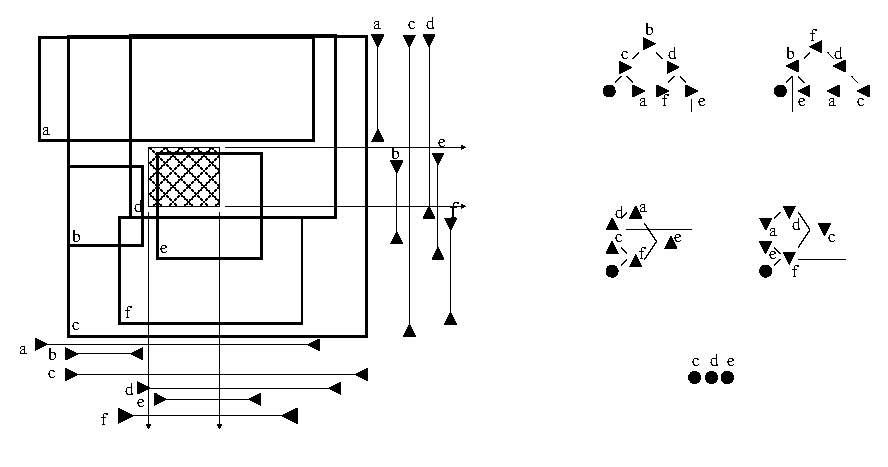
\includegraphics{figs/dct.fig.eps}%
\end{picture}%
\setlength{\unitlength}{4144sp}%
%
\begingroup\makeatletter\ifx\SetFigFont\undefined%
\gdef\SetFigFont#1#2#3#4#5{%
  \reset@font\fontsize{#1}{#2pt}%
  \fontfamily{#3}\fontseries{#4}\fontshape{#5}%
  \selectfont}%
\fi\endgroup%
\begin{picture}(6507,3300)(76,-2506)
\put(991,-2491){\makebox(0,0)[lb]{\smash{{\SetFigFont{8}{9.6}{\familydefault}{\mddefault}{\updefault}{\color[rgb]{0,0,0}\wxn}%
}}}}
\put(1531,-2491){\makebox(0,0)[lb]{\smash{{\SetFigFont{8}{9.6}{\familydefault}{\mddefault}{\updefault}{\color[rgb]{0,0,0}\wxx}%
}}}}
\put(3601,-196){\makebox(0,0)[lb]{\smash{{\SetFigFont{8}{9.6}{\familydefault}{\mddefault}{\updefault}{\color[rgb]{0,0,0}\wyx}%
}}}}
\put(3601,-691){\makebox(0,0)[lb]{\smash{{\SetFigFont{8}{9.6}{\familydefault}{\mddefault}{\updefault}{\color[rgb]{0,0,0}\wyn}%
}}}}
\put(4141,-1456){\makebox(0,0)[lb]{\smash{{\SetFigFont{9}{10.8}{\rmdefault}{\mddefault}{\updefault}{\color[rgb]{0,0,0}$y$-dim trees include CQ regions that overlap}%
}}}}
\put(5131,-1636){\makebox(0,0)[lb]{\smash{{\SetFigFont{9}{10.8}{\rmdefault}{\mddefault}{\updefault}{\color[rgb]{0,0,0}in $x$ dimension.}%
}}}}
\put(4681,-241){\makebox(0,0)[lb]{\smash{{\SetFigFont{9}{10.8}{\rmdefault}{\mddefault}{\updefault}{\color[rgb]{0,0,0}$x$-dim trees include all CQ regions}%
}}}}
\put(4321,-2221){\makebox(0,0)[lb]{\smash{{\SetFigFont{9}{10.8}{\rmdefault}{\mddefault}{\updefault}{\color[rgb]{0,0,0}\A\ includes regions overlapping in $x$ and $y$}%
}}}}
\put(5266,-871){\makebox(0,0)[lb]{\smash{{\SetFigFont{9}{10.8}{\rmdefault}{\mddefault}{\updefault}{\color[rgb]{0,0,0}\wyx}%
}}}}
\put(5266,-691){\makebox(0,0)[lb]{\smash{{\SetFigFont{9}{10.8}{\rmdefault}{\mddefault}{\updefault}{\color[rgb]{0,0,0}\Yn}%
}}}}
\put(6436,-1096){\makebox(0,0)[lb]{\smash{{\SetFigFont{9}{10.8}{\rmdefault}{\mddefault}{\updefault}{\color[rgb]{0,0,0}\wyn}%
}}}}
\put(6391,-691){\makebox(0,0)[lb]{\smash{{\SetFigFont{9}{10.8}{\rmdefault}{\mddefault}{\updefault}{\color[rgb]{0,0,0}\Yx}%
}}}}
\put(5131,-61){\makebox(0,0)[lb]{\smash{{\SetFigFont{9}{10.8}{\rmdefault}{\mddefault}{\updefault}{\color[rgb]{0,0,0}\wxx}%
}}}}
\put(5311,524){\makebox(0,0)[lb]{\smash{{\SetFigFont{9}{10.8}{\rmdefault}{\mddefault}{\updefault}{\color[rgb]{0,0,0}\Xn}%
}}}}
\put(6481,569){\makebox(0,0)[lb]{\smash{{\SetFigFont{9}{10.8}{\rmdefault}{\mddefault}{\updefault}{\color[rgb]{0,0,0}\Xx}%
}}}}
\put(5896,-61){\makebox(0,0)[lb]{\smash{{\SetFigFont{9}{10.8}{\rmdefault}{\mddefault}{\updefault}{\color[rgb]{0,0,0}\wxn}%
}}}}
\put(5896,-1996){\makebox(0,0)[lb]{\smash{{\SetFigFont{9}{10.8}{\rmdefault}{\mddefault}{\updefault}{\color[rgb]{0,0,0}\A}%
}}}}
\end{picture}%
}
  \caption[\acf{DCT} with windows]{%
    \acf{DCT} with six CQ \acp{ROI}, $a, b, \ldots, f$.  Shown are the
    indexed \acp{ROI}, the current window, and the cascading trees,
    \Xn, \Xx, \Yn, \Yx, \id{A}, and the window node pointers, \wxn,
    \wxx, \wyn, \wyx\ that make up the data structure.}
  \label{fig:dct}
\end{figure}

The \ac{DCT} maintains separate trees for both the minimum and maximum
endpoints of each of the \ac{CQ} \acp{ROI} for each dimension.  In
Figure~\ref{fig:dct}, these are denoted as \Xn\ and \Xx\ for the
$x$-direction, and \Yn\ and \Yx\ for the $y$-direction.  These are
termed \emph{endpoint trees} in the \ac{DCT}.  A final tree, \id{A}, maintains
an index of all the \acp{ROI} that overlap with the current data
in the input stream.  The figure shows these trees notionally,
emphasizing their ordering and structure; the endpoint trees using one
endpoint and the \rid, and the \id{A} tree only using \rid.  The values
of the nodes contain pointers back to the \acp{ROI}, or the
associated \ac{CQ} query in the \ac{DSMS}.

Which of the \ac{CQ} \acp{ROI} are included in the trees varies with the
dimension.  The trees for the first dimension, $x$, contain the
minimum (in \Xn) and maximum (in \Xx) endpoints for \emph{every}
\ac{CQ} \ac{ROI}.  \Yn\ and \Yx\ do not contain the endpoints of all the
\acp{ROI} in \ac{DCT}, but only \emph{the \acp{ROI} with $x$ extents that overlap
  the current data stream's $x$ extents}.

This is easily expanded to more dimensions, where each additional
dimension adds another set of trees to the \ac{DCT} that hold the
minimum/maximum endpoints of the \ac{CQ} \acp{ROI} in this new
dimension.  Again, each of these new trees only index those \acp{ROI}
that overlap the current window up to that dimension.

\id{A} is the final tree and contains all the \acp{ROI} that overlap with
the current window in all dimensions.  Just as the trees in the
$y$-dimension contain only a subset of the \acp{ROI} that are indexed in
the $x$-dimension, \id{A} contains the subset of the \acp{ROI} where the
$y$-dimension of the window and the \ac{CQ} \acp{ROI} overlap.  \id{A}
contains \acp{ROI} that overlap with the window query in every
dimension, and therefore these \acp{ROI} intersect the current query
window.  These tree structures in each dimension make a cascade of
indexes, each a subset of the previous index.

In addition, pointers identifying where the current window is located
are maintained.  This is accomplished by pointing to nodes within each
of the endpoint trees for each of the dimensions in the \ac{DCT}.  The
pointers match the closest endpoint with a value less than or equal to
current window location.  These are pointers to existing nodes and not
the actual values of the window endpoints themselves.  Since nodes
correspond to line segments, these identify regions where the current
result set is still valid.

Figure~\ref{fig:dct} shows these pointers in each dimension.  They are
designated as \wxn\ and \wxx\ for the $x$-dimension, and \wyn\ and
\wyx\ for the $y$-dimension.  Note that the minimum window endpoints,
for example \wxn, point into the tree of maximum endpoints for the
\ac{CQ} \acp{ROI}.  Similarly, the maximum window pointers are in the
trees of minimum endpoints.  This is more fully explained in
Section~\ref{sec:query} describing how the \ac{DCT} returns \ac{CQ}
\acp{ROI} for new data extents, but in short imagine as a spatial extent
grows in size, new \ac{CQ} \acp{ROI} would become added to the result
set as the maximum edge of the extent crosses the minimum edge of new
\acp{ROI}.  Similarly, \acp{ROI} would be added as the data extent minimum
crosses new region maximum edges.  The same idea applies for shrinking
edges.  Tracking the movement of the spatial extents of the incoming
data stream from query to query is how the \ac{DCT} incrementally
maintains a result set of intersecting \ac{CQ} \acp{ROI}.

The individual components of the \ac{DCT} can be implemented using simple
binary tree structures.  The structures need to support insertion,
deletion, and iteration of nodes in both forward and reverse
directions.  These can be implemented by \ac{STL}~\cite{99stand-templ}
objects like \emph{set} or \emph{map}, or by similar structures like a
slightly modified skip list~\cite{pugh90skip}.  The endpoint trees use
keys for each node are made up from two values, one corresponding to
an endpoint value for each \ac{CQ} \ac{ROI} in one dimension, and
another corresponding to a unique identifier for each \ac{ROI},
\rid.  The two values are combined so that spatial order is
maintained.  Different \ac{CQ} \acp{ROI} that share an endpoint value
are differentiated with the \rid's.  Individual nodes correspond to
the half-open line segments between two endpoints in a single
dimension.  The trees all have an additional node with a minimum
endpoint that is less than any possible region, shown as a dot in the
trees of Figure~\ref{fig:dct}.  These allow half-open line segments to
completely cover a potential location of the incoming data stream.

\subsection{Initialization}

The \ac{DCT} is initialized by creating the minimum/maximum endpoint
trees for each dimension of the \ac{DCT}.  Initial nodes for each endpoint
tree are created by adding a node with a value that is less than any
possible value for a region in each dimension.  These are
shown as dots in the trees of Figure~\ref{fig:dct}.

The current window location is then created by assigning the pointers
\wxn, \wxx, \wyn, and \wyx\ to the appropriate minimum node for each of
the endpoint trees in each dimension.  The \id{A} structure is initially
empty.

\subsection{Inserting and Deleting \acp{ROI}}

Insertion and deletion of \ac{CQ} \acp{ROI} are simple routines. For
insertion of a new \ac{ROI} $r$, first the $x$-dimension endpoints are
inserted into \Xn\ and \Xx.  The new \ac{ROI} is checked for overlap
with current stream data extents, that is both $\wxn < r_{x+}$ and
$\wxx >= r_{x-}$ hold, where $r_{x+}$ and $r_{x-}$ are the maximum and
minimum values of the new \ac{ROI} in the $x$ dimension.  If the new
\ac{ROI} does overlap the current window, then \ac{ROI} is also added into
trees \Yn\ and \Yx.  If the new \ac{ROI} overlaps in this dimension,
$\wyn < r_{y+}$ and $\wyx >= r_{y-}$, then the \ac{ROI} is added into
\id{A} using \rid\ as the index.  Insertion maintains the validity of the
result set, \id{A} with respect to the current data stream window.

Deletion is similar, following the cascade of the \ac{DCT}, with one
modification.  The current window pointers need to be checked to
verify that they are not pointing to a node that is being removed.  If
they are then they need to be modified.  For example, to delete \ac{ROI}
$r$, if \wxx\ points to this \ac{ROI}, then decrement \wxx\ to the
previous node in \Xn.  If \wxn\ points to the maximum endpoint of $r$,
then decrement \wxn\ to the previous point in \Xx.  These changes
maintain the validity for \Yn, \Yx, and \id{A}.  The endpoints of $r$ are
then deleted from \Xn\ and \Xx.  If the \ac{ROI} intersects the current
window, it needs to be deleted in a similar manner from \Yn\ and \Yx,
and potentially \id{A} as well.

\subsection{Queries}
\label{sec:query}

\begin{figure}[htb]
  \centering
  \begin{picture}(0,0)%
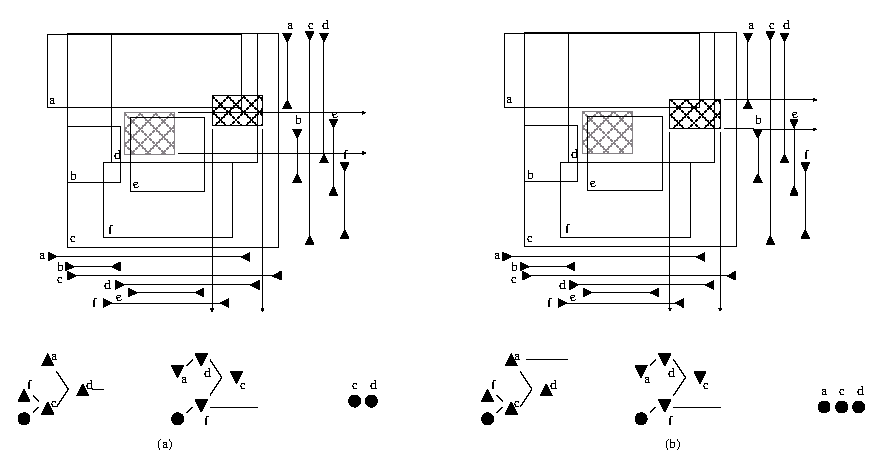
\includegraphics{figs/move.fig.eps}%
\end{picture}%
\setlength{\unitlength}{4144sp}%
%
\begingroup\makeatletter\ifx\SetFigFont\undefined%
\gdef\SetFigFont#1#2#3#4#5{%
  \reset@font\fontsize{#1}{#2pt}%
  \fontfamily{#3}\fontseries{#4}\fontshape{#5}%
  \selectfont}%
\fi\endgroup%
\begin{picture}(6478,3331)(191,-2492)
\put(5457,-1512){\makebox(0,0)[lb]{\smash{{\SetFigFont{7}{8.4}{\familydefault}{\mddefault}{\updefault}{\color[rgb]{0,0,0}\wxx}%
}}}}
\put(5074,-1512){\makebox(0,0)[lb]{\smash{{\SetFigFont{7}{8.4}{\familydefault}{\mddefault}{\updefault}{\color[rgb]{0,0,0}\wxn}%
}}}}
\put(6337,182){\makebox(0,0)[lb]{\smash{{\SetFigFont{7}{8.4}{\familydefault}{\mddefault}{\updefault}{\color[rgb]{0,0,0}\wyx}%
}}}}
\put(6337,-42){\makebox(0,0)[lb]{\smash{{\SetFigFont{7}{8.4}{\familydefault}{\mddefault}{\updefault}{\color[rgb]{0,0,0}\wyn}%
}}}}
\put(901,-1771){\makebox(0,0)[lb]{\smash{{\SetFigFont{7}{8.4}{\rmdefault}{\mddefault}{\updefault}{\color[rgb]{0,0,0}\Yn}%
}}}}
\put(2071,-2176){\makebox(0,0)[lb]{\smash{{\SetFigFont{7}{8.4}{\rmdefault}{\mddefault}{\updefault}{\color[rgb]{0,0,0}\wyn}%
}}}}
\put(2026,-1771){\makebox(0,0)[lb]{\smash{{\SetFigFont{7}{8.4}{\rmdefault}{\mddefault}{\updefault}{\color[rgb]{0,0,0}\Yx}%
}}}}
\put(901,-2041){\makebox(0,0)[lb]{\smash{{\SetFigFont{7}{8.4}{\rmdefault}{\mddefault}{\updefault}{\color[rgb]{0,0,0}\wyx}%
}}}}
\put(2746,-1771){\makebox(0,0)[lb]{\smash{{\SetFigFont{7}{8.4}{\rmdefault}{\mddefault}{\updefault}{\color[rgb]{0,0,0}\A}%
}}}}
\put(4433,-1816){\makebox(0,0)[lb]{\smash{{\SetFigFont{7}{8.4}{\rmdefault}{\mddefault}{\updefault}{\color[rgb]{0,0,0}\wyx}%
}}}}
\put(4433,-2266){\makebox(0,0)[lb]{\smash{{\SetFigFont{7}{8.4}{\rmdefault}{\mddefault}{\updefault}{\color[rgb]{0,0,0}\Yn}%
}}}}
\put(5603,-2176){\makebox(0,0)[lb]{\smash{{\SetFigFont{7}{8.4}{\rmdefault}{\mddefault}{\updefault}{\color[rgb]{0,0,0}\wyn}%
}}}}
\put(5558,-1771){\makebox(0,0)[lb]{\smash{{\SetFigFont{7}{8.4}{\rmdefault}{\mddefault}{\updefault}{\color[rgb]{0,0,0}\Yx}%
}}}}
\put(6323,-1771){\makebox(0,0)[lb]{\smash{{\SetFigFont{7}{8.4}{\rmdefault}{\mddefault}{\updefault}{\color[rgb]{0,0,0}\A}%
}}}}
\put(1618,-1514){\makebox(0,0)[lb]{\smash{{\SetFigFont{6}{7.2}{\familydefault}{\mddefault}{\updefault}{\color[rgb]{0,0,0}\wxn}%
}}}}
\put(2001,-1514){\makebox(0,0)[lb]{\smash{{\SetFigFont{6}{7.2}{\familydefault}{\mddefault}{\updefault}{\color[rgb]{0,0,0}\wxx}%
}}}}
\end{picture}%

  \caption[Query on a new region]{%
    Query on a new region. The original window position (as in
    Figure~\ref{fig:dct}) is shown in grey, and the new region in black.
    (a) shows the updated \Yn,\Yx, and \id{A} structures after moving the
    window in $x$.  (b) shows the final structures after moving
    in $y$.}
  \label{fig:update}
\end{figure}

Figure~\ref{fig:update} describes the changes to the \ac{DCT} for new
stream data with new extents.  As \Xn\ and \Xx\ are not changed, only
the values of \Yn, \Yx, and \id{A} are shown.  Figure~\ref{fig:update}(a)
shows the query change due to the movement in the $x$ dimension and
\ref{fig:update}(b) shows the change due to the movement in the $y$
dimension.  Just as the trees for each dimension and \id{A} need to be
maintained when new \acp{ROI} are inserted and deleted, each new window
query requires maintenance of these trees as the window changes its
location.  These changes are made incrementally on the existing
structure of the \ac{DCT}.

Since \Yn\ and \Yx\ contain \acp{ROI} overlapping the current window's
$x$ extent, when new data arrives with different $x$-extents,
\Yn,\Yx, and \id{A} need to be modified.  These modifications occur when
the window region end points cross a boundary of \ac{CQ} \ac{ROI}.  For
each $x$ \ac{ROI} boundary in the \ac{DCT} that is crossed, the
$y$-dimensional trees need to be modified to account for inclusion or
deletion of this new \ac{ROI}.  A similar method needs to be associated
with boundary crossings in the $y$-dimension,
% while the windows projection in the $y$ dimension changes, 
requiring modification of \id{A}.

The algorithm for reporting overlapping \ac{CQ} \acp{ROI} for window,
$w~=~((\wxn, \wyn)$, $(\wxx, \wyx))$ begins by traversing the
endpoint trees in the $x$ direction.  Figure~\ref{fig:update}(a) shows
an example where the new query region has increasing minimum and
maximum $x$ edges.  An increasing minimum edge implies that the
movement can result in \acp{ROI} being deleted from the result set.
The movement of \wxn\ is tracked by incrementing along the nodes of
\Xx.  Moving \wxn\ to a new node corresponds to a boundary crossing of
the window minimum with a region maximum, and in this case corresponds
to one \ac{ROI}, $e$, being removed from \Yn\ and \Yx.  This deletion
is cascaded to \id{A} as well.  The increasing maximum, \wxx,
corresponds to a movement that would add \acp{ROI}.  However, in this
case, although the window maximum is greater, no minimum nodes are
crossed, and \wxx\ remains pointing to the minimum node, of \ac{ROI}
$e$, as in Figure~\ref{fig:dct}.  The net result of moving the window
in the $x$ direction is that \ac{ROI} $e$ is removed from \Yn, \Yx,
and \id{A}.

Next, the movement of the window in the $y$ direction is accounted for
as shown in Figure~\ref{fig:update}(b).  In this case, although the
$y$ minimum of the window has changed, no maximum boundaries are
crossed, and \wyn\ remains pointing to the maximum value of \ac{ROI} $f$.
Moving the window maximum in $y$, however, results in the minimum edge
of \ac{ROI} $a$ to be crossed.  \wyx\ now points to the minimum edge of
$a$, and $a$ is added to the result set \id{A}.

This example shows one type of movement of the window region, but the
same algorithm works for all changes of the window region.  The window
can grow and contract on all sides, or move in any direction.  The
algorithm works the same way; each edge of the window query is handled
separately either adding to or deleting from the subsequent trees and
the final result, based on the direction of movement of the edge.

There is one caveat to this algorithm for updating the \ac{DCT} based on
the movement of edges individually.  Without modification of the above
algorithm, the expansive movements of the new window query need to be
performed before the shrinking movements.  Large movements of the
window can produce movements across both edges of an \ac{CQ} \ac{ROI}.
Expanding first prevents a \ac{ROI} from being deleted first on a
shrinking movement, and then erroneously inserted on expansion.
Executing deletions first however decreases the size of the trees in
the \ac{DCT}.  To allow shrinking movements first, during the expansive
movements, range checks are done to verify the \ac{ROI} indeed belongs
in the overlapping set before inserting it into subsequent trees.

%%%%%%%%%%%%%%%%%%%%%%%%%%%%%%%%%%%%%%%%%%%%%%%%%%%%%%%%%%%%%%%%%%%%%%

%%%%%%%%%%%%%%%%%%%%%%%%%%%%%%%%%%%%%%%%%%%%%%%%%%%%%%%%%%%%%%%%%%%%%%
%%%%%%%%%%%%%%%%%%%%%%%%%%%%%%%%%%%%%%%%%%%%%%%%%%%%%%%%%%%%%%%%%%%%%%
\section{\ac{DCT} Performance}
\label{sec:performance}

The window query performance of the \ac{DCT} is highly dependent on the
location of the \acp{ROI}, the properties of the incoming window
queries, and the interaction of these parameters.  For queries over
$n$ \acp{ROI}, with $k$ being the result count, the execution
time for window query can range from $O(k)$ in the best case, when the
result set is the same as the previous set to $O(n\lg{n}+k)$ in the
worst case, when every \ac{ROI} is entered in a single movement
of the incoming spatial extents.  Before looking at some experimental
results, there are some simple guidelines to consider for the
application of the \ac{DCT}.

\subsection{\ac{ROI} Insertion and Deletion Cost}

The \ac{DCT} data structure is small and robust to many insertions and
deletions of \ac{CQ} \acp{ROI}.  Insertions and deletions take
$O(\lg{n})$ time as the query \ac{ROI} is potentially added to the
endpoint trees in some constant dimension and \id{A}.  These trees
are simple to maintain dynamically in $O(n)$ space.

\subsection{Cost Versus the Number of Boundaries Crossed}

The \ac{DCT} is designed for trending data, which can 
be measured by the number of \ac{ROI} boundary crossings from
one window query to the next. The structure works best when the
number of \ac{ROI} boundaries crossed by successive queries is not
large.  When no boundaries are crossed, then no internal lists are
modified, and reporting \acp{ROI} runs in $O(k)$ time.  When a boundary
is crossed in movement of the window query, then each \ac{ROI}
with a crossed boundary needs to be inserted into or deleted from
subsequent endpoint trees.  This is true for at least one set of
endpoint trees or \id{A}, even for \ac{CQ} \acp{ROI} whose domains in other
dimensions do not overlap the new window and thus do not contribute to
the final result.  The cost of a window query in this case can be as
high as $O(n\lg{n} + k)$, since all \acp{ROI} could potentially be
inserted into dimensional trees during one window query.

The \ac{DCT} data structure does indexing somewhat lazily in the sense
that for insertions of new \acp{ROI} that do not overlap the
current window, only the first dimension is indexed, and not the
other dimensions.  The indexing costs on window queries can be thought
of as finally incurring those indexing costs.  However, the problem
with the \ac{DCT} is that these costs can occur many times in the motion
of the input stream.  Rather than indexing \ac{ROI} values once, the
\ac{DCT} re-indexes a subset of points multiple times as boundaries are
crossed.  The hope is that many successive window queries will be in
the same \ac{ROI} with the same result, and that the low cost for those
queries will make up for the extra cost of maintaining a dynamic
index.

\subsection{Trajectory of the Trending Windows}

Another aspect affecting performance is the movement trajectory of the
window queries.  For example, consider a \ac{DCT} in two dimensions like
that shown in Figure~\ref{fig:dct} with trajectories that are
monotonic in the $x$ and $y$ dimensions.  In this case, \acp{ROI} are
inserted into the $y$ endpoint trees and \id{A} at most one time, and
once more potentially for deletion.  The total time for maintaining
the \ac{DCT} then is at most $O(n\lg{n})$, fixing a bound on the dynamic
maintenance costs.  For $m$ window queries over that trajectory, the
cost of all queries would be $O(n\lg{n}+mk)$ where $k$ is the average
number of results per query.  In comparison, for two-dimensional
segment tree implementation, the total cost would be
$O(n\lg^2{n}+m\lg^2{n}+mk)$, where $n\lg^2{n}$ is the cost of building
a static segment tree.  Similar savings exist for trajectories that
are generally monotonic, such as most \ac{RSI} data streams.

On the other hand, more erratic window trajectories can result in poor
performance.  Consider a window movement that repeatedly crosses all
$n$ \ac{ROI} boundaries.  Each query iteration would require
$O(n\lg{n})$ time, as the $y$ dimensional trees are repeatedly made up
and torn down.

Also, the \ac{DCT} as described in Figures~\ref{fig:dct} and
\ref{fig:update}, which indexes on $x$ and then $y$, favor window that
trend in the $y$ direction over windows that trend in the $x$
direction.  This is because boundary crossings in the $x$ dimension
have to modify more trees, and the tress tend to be bigger, so they
take more time.  Movements in the $y$ dimension only modify \id{A}, a
single tree that is the smallest tree in the \ac{DCT}.  Also,
movements in the $x$ direction result in insertions into \Yn\ and \Yx\
which can be somewhat wasted in the sense that these \acp{ROI} may
never contribute to a final result set, whereas boundary crossings in
the $y$ direction will always affect the result set.  Although, the
time it takes to update the \ac{DCT} due to a boundary crossing is
$O(\lg{n})$, for either $x$ or $y$ dimension, $y$ modifications will
always be faster.

This shows that order in the cascade is very important, and dimensions
that see more boundary crossings for successive window queries into
the \ac{DCT} should be pushed deeper into the structure.  Boundary
crossings are of course dependent on the trajectory of window queries
and the organization of the \acp{ROI} in the \ac{DCT}.
Section~\ref{sec:experiments} reports on indexing tests on the
\ac{DCT} and quantifies some of the performance features identified in
this section.

\subsection{Skipping Worthless Insertions}
%
When the next window of the input stream trends a long way with
respect to the number of query boundaries traversed, then the time for
reporting queries goes up to at least the number of \acp{ROI} contained
in all the boundaries crossed.  \acp{ROI} that are both entered and
exited in the course of a single traversal to a new window are even
worse.  Their endpoints are needlessly added, then deleted from the
\ac{DCT}, at a cost of up to $O(\lg{n})$, and never queried.  This can
easily be remedied, but for clarity was left out of the initial
\proc{Update-Ith} algorithm.  When encountering a \ac{ROI} at a boundary
crossing, check that the \ac{ROI} will remain a valid \ac{ROI} in the
first dimension when the window has finished its traversal before
inserting into the next structure.  This prevents wasted index
modifications, but does not help with the basic problem of long
traverses or input windows that cross back and forth across expensive
boundaries.

\section{Experiments}
\label{sec:experiments}

To test the performance of the \ac{DCT}, two experimental setups were
used.  The first tests are on randomly moving data stream and random
\ac{CQ} \acp{ROI}, with a number of variations on specific input
parameters.  The second experiment was developed to more closely
replicate the queries made on a \ac{DSMS} with \ac{GOES} \ac{RSI} data
as input, and more realistic \ac{ROI} parameters.

Comparisons were made to an existing in memory R*-tree implementation
from the \emph{Spatial Index Library}~\cite{hadjiel04spatial-index}.
For better comparison, the \ac{DCT} implementation included some
components from this same library.  All trees in this implementation
of the \ac{DCT} were simple set objects from the
\acf{STL}~\cite{99stand-templ}.  The total size of this experimental
\ac{DCT} implementation was about 600 lines of C++ code.  All experiments
were run on a single 1.6 GHz Pentium M CPU with a 1MB L2 cache and
512MB of main memory.


\subsection{Random Continuous Queries with a Random Data Stream}
\label{sec:random}

The more extensive tests were run using a set of \ac{CQ} \acp{ROI} that
were randomly located throughout a two dimensional space, with some
variation of parameters as shown in Figure~\ref{fig:random}.  For most
tests, the input data stream moved randomly though the region, with
the default parameters also shown in Figure~\ref{fig:random}.  The
\ac{CQ} \acp{ROI} were distributed uniformly throughout a square region.
Some region parameters are modified for certain tests, these tables
show the default values.  Aspect is the ratio of lengths $\frac{x}{y}$
of the \ac{CQ} \acp{ROI} or the spatial extent of data from the input
stream.  For most tests, the window query moved in a random direction
from one query to the next.

Sometimes, the extents of the input stream would trend off test area.
When this occurred, a new starting point within the region was chosen
to reset the window location.

These experiments do not correspond closely to any real world
application, but are instructive in testing the performance of the
\ac{DCT} with respect to various parameters.  All experiments plot the
average response time for a window query as a function of a single
parameter.  All experiments were run using 4K and 16K \ac{CQ} \acp{ROI}.
%
\begin{figure}[htb]
  \subfigure[Random test parameters]{
    \begin{minipage}[b]{7.5cm}
      \begin{minipage}[c]{2,5cm}
        \vspace{0pt}
        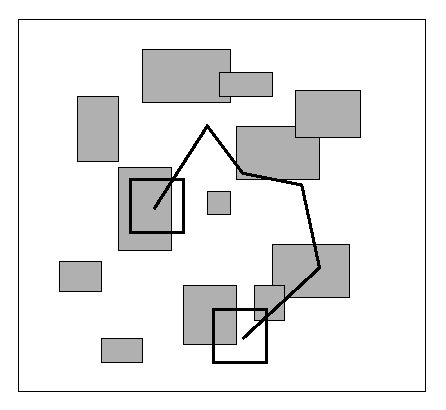
\includegraphics[width=2.45cm]{figs/random_tests.fig.eps}%
      \end{minipage}
      \begin{minipage}[c]{3.5cm}
        \begin{tabular}[t]{|cl|}
          \multicolumn{2}{c}{Default \ac{ROI} parameters} \\
          \hline
          Area & 0.1-10 [\%] \\
          Aspect & 0.7-1.4 \\
          \hline
          \multicolumn{2}{c}{Default query parameters} \\
          \hline
          Area & 1 [\%]\\
          Aspect & 1 \\
          Distance & 1 [\%] \\
          \hline
        \end{tabular}
      \end{minipage}
      \vspace{0pt}
    \end{minipage}
    \label{fig:random}
  }
  \subfigure[Query times vs. distance between subsequent queries.]{
    \scalebox{0.85}{%GNUPLOT: LaTeX picture with Postscript
\begin{picture}(0,0)%
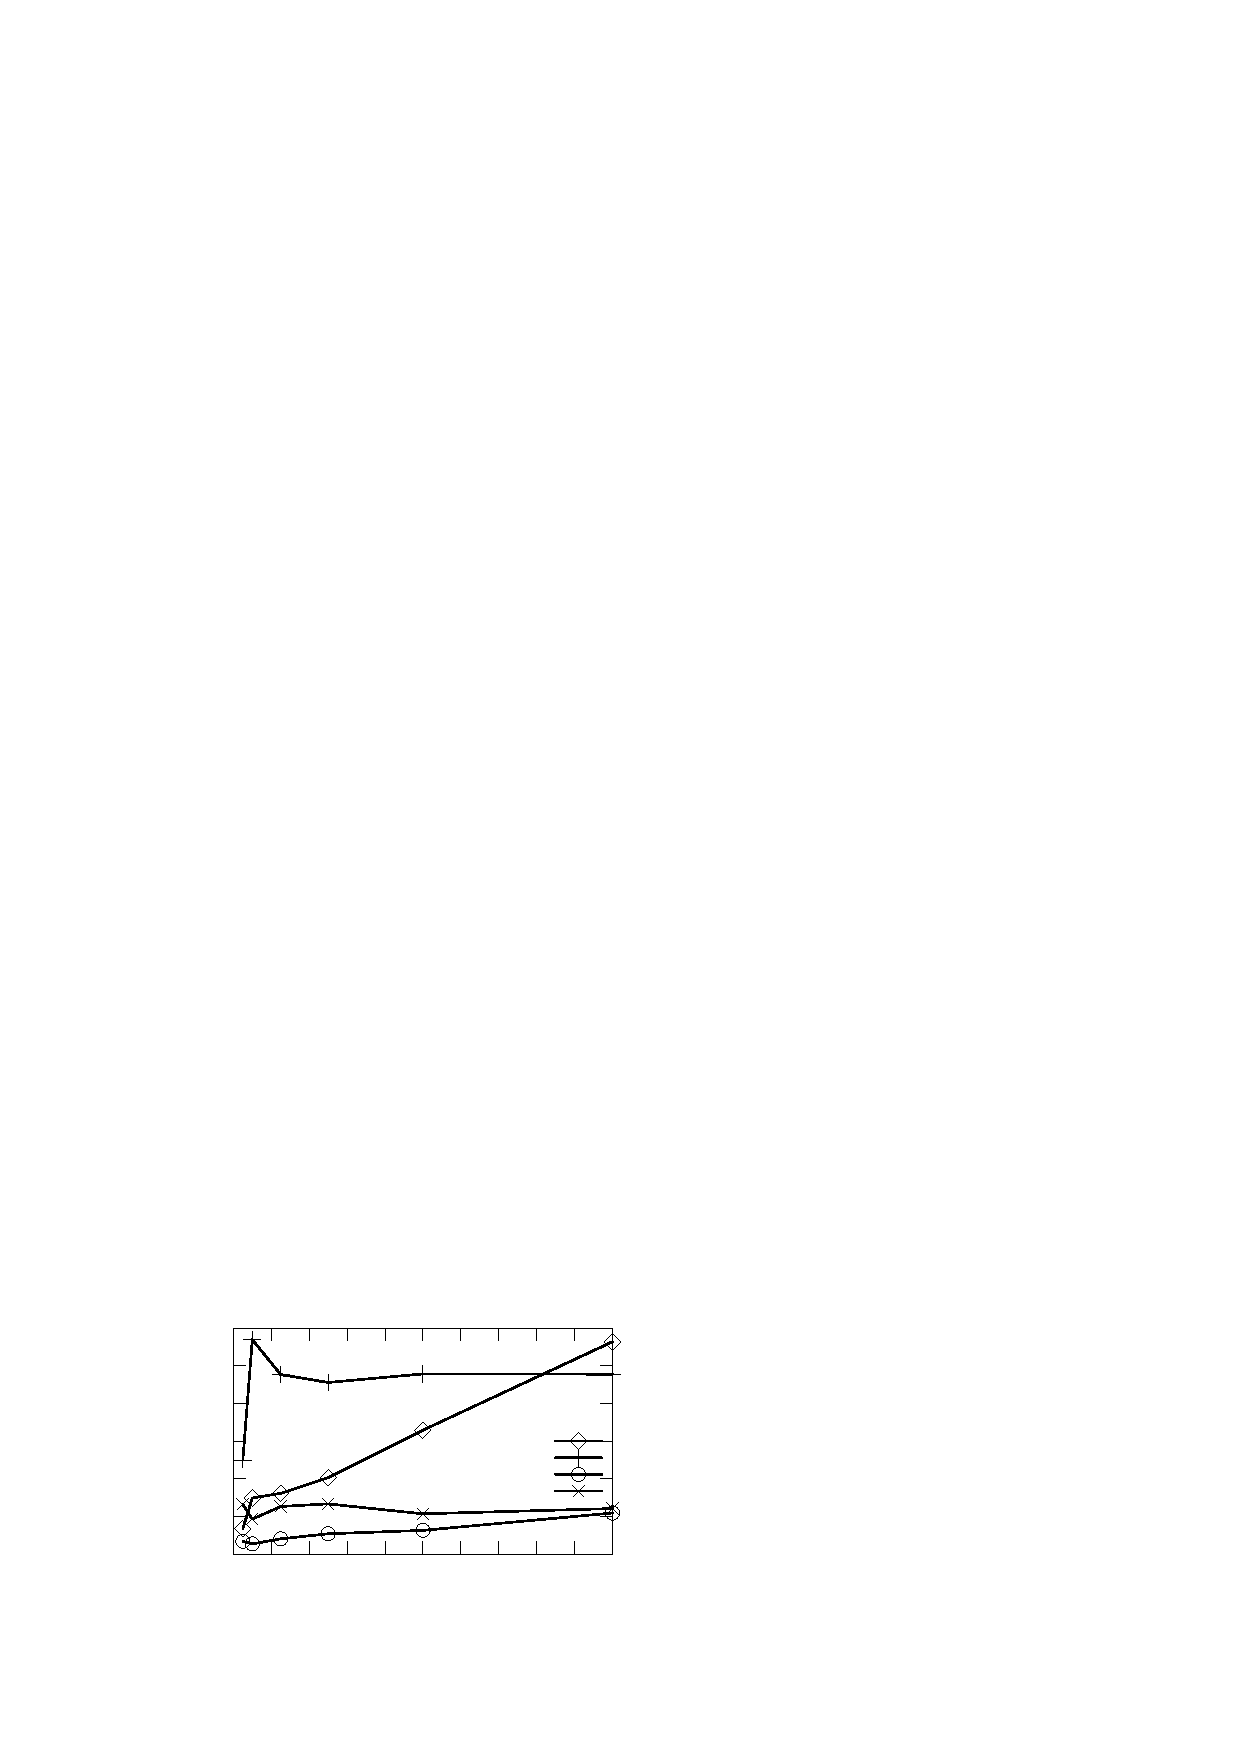
\includegraphics{dis}%
\end{picture}%
\begingroup
\setlength{\unitlength}{0.0200bp}%
\begin{picture}(11699,7019)(0,0)%
\put(1800,1200){\makebox(0,0)[r]{\strut{} 0}}%
\put(1800,2103){\makebox(0,0)[r]{\strut{} 1000}}%
\put(1800,3007){\makebox(0,0)[r]{\strut{} 2000}}%
\put(1800,3910){\makebox(0,0)[r]{\strut{} 3000}}%
\put(1800,4813){\makebox(0,0)[r]{\strut{} 4000}}%
\put(1800,5717){\makebox(0,0)[r]{\strut{} 5000}}%
\put(1800,6620){\makebox(0,0)[r]{\strut{} 6000}}%
\put(2000,800){\makebox(0,0){\strut{} 0}}%
\put(2910,800){\makebox(0,0){\strut{} 0.2}}%
\put(3820,800){\makebox(0,0){\strut{} 0.4}}%
\put(4730,800){\makebox(0,0){\strut{} 0.6}}%
\put(5640,800){\makebox(0,0){\strut{} 0.8}}%
\put(6550,800){\makebox(0,0){\strut{} 1}}%
\put(7460,800){\makebox(0,0){\strut{} 1.2}}%
\put(8370,800){\makebox(0,0){\strut{} 1.4}}%
\put(9280,800){\makebox(0,0){\strut{} 1.6}}%
\put(10190,800){\makebox(0,0){\strut{} 1.8}}%
\put(11100,800){\makebox(0,0){\strut{} 2}}%
\put(400,3910){\rotatebox{90}{\makebox(0,0){Time [$\mu s$]}}}%
\put(6550,200){\makebox(0,0){Distance Moved [\%]}}%
\put(9535,3910){\makebox(0,0)[r]{\strut{}DCT-16K}}%
\put(9535,3510){\makebox(0,0)[r]{\strut{}RTREE-16K}}%
\put(9535,3110){\makebox(0,0)[r]{\strut{}DCT-4K}}%
\put(9535,2710){\makebox(0,0)[r]{\strut{}RTREE-4K}}%
\end{picture}%
\endgroup
\endinput
}
    \label{fig:dis} 
  }
  \caption{Test parameters and distance test}
\end{figure}

Figure~\ref{fig:dis} shows the average window query time while varying
the average distance moved from on window query to another.  The
direction of the move was randomly determined.  This is one of the
most important parameters to consider when using the \ac{DCT}.  The window
queries must come close to one another for the index to work
effectively.  As expected, while the R*-tree is insensitive to this
parameter, the \ac{DCT} performance is very dependent on the distance
moved for a window query.  As the distance between window queries
increases, the amount of information that can be shared in the trees
of the \ac{DCT} become less and less.  For data in the input stream at a
size of 1\% of the total area, a move over a distance of 2\% virtually
eliminates all sharing of information between queries.  At what point
the distance between queries becomes limiting is dependent on other
application parameters.  For example, as more \acp{ROI} are added into
the \ac{DCT}, more boundaries are likely to be crossed over the same
distance moved.


The size of the stream data extents also affects the performance of
the \ac{DCT}.  In general, larger extents in the data from the incoming
stream would be expected to share more results from query to query and
therefore improve the performance of the \ac{DCT}.
Figure~\ref{fig:stab_area} compares the \ac{DCT} to the R*-tree for
different size extents in the incoming stream.  The average response
time increases for both implementations, but less so for the \ac{DCT}.
For this experiment, the result sets for the window queries increases
with window query size as well, so it is expected that the response
time increases with stream data extents.  The \ac{DCT} results are somewhat
artificially high for another reason.  As was described, the query
window is relocated to a new random location when the window trends
off the experiment's region.  Since this is more likely to occur with
larger stream extents, more of these relocations occur in those
experiments and since each relocation corresponds to larger query
distance movements in the \ac{DCT}, this increases the average distance
between data in the stream.

As described in the introduction, the intent of the \ac{DCT} is for use
in streaming \ac{RSI}, and these usually entail incoming data packets
of a row, or small number of rows of data.  Since these correspond to
the extents of the individual data in the incoming geospatial data
stream, \ac{DCT} queries can have a high aspect ratios, that is,
$\frac{x}{y} \gg 1$.
%
\begin{figure}[htb]
\subfigure[Query times vs. area of the window query.]{
    \scalebox{0.85}{%GNUPLOT: LaTeX picture with Postscript
\begin{picture}(0,0)%
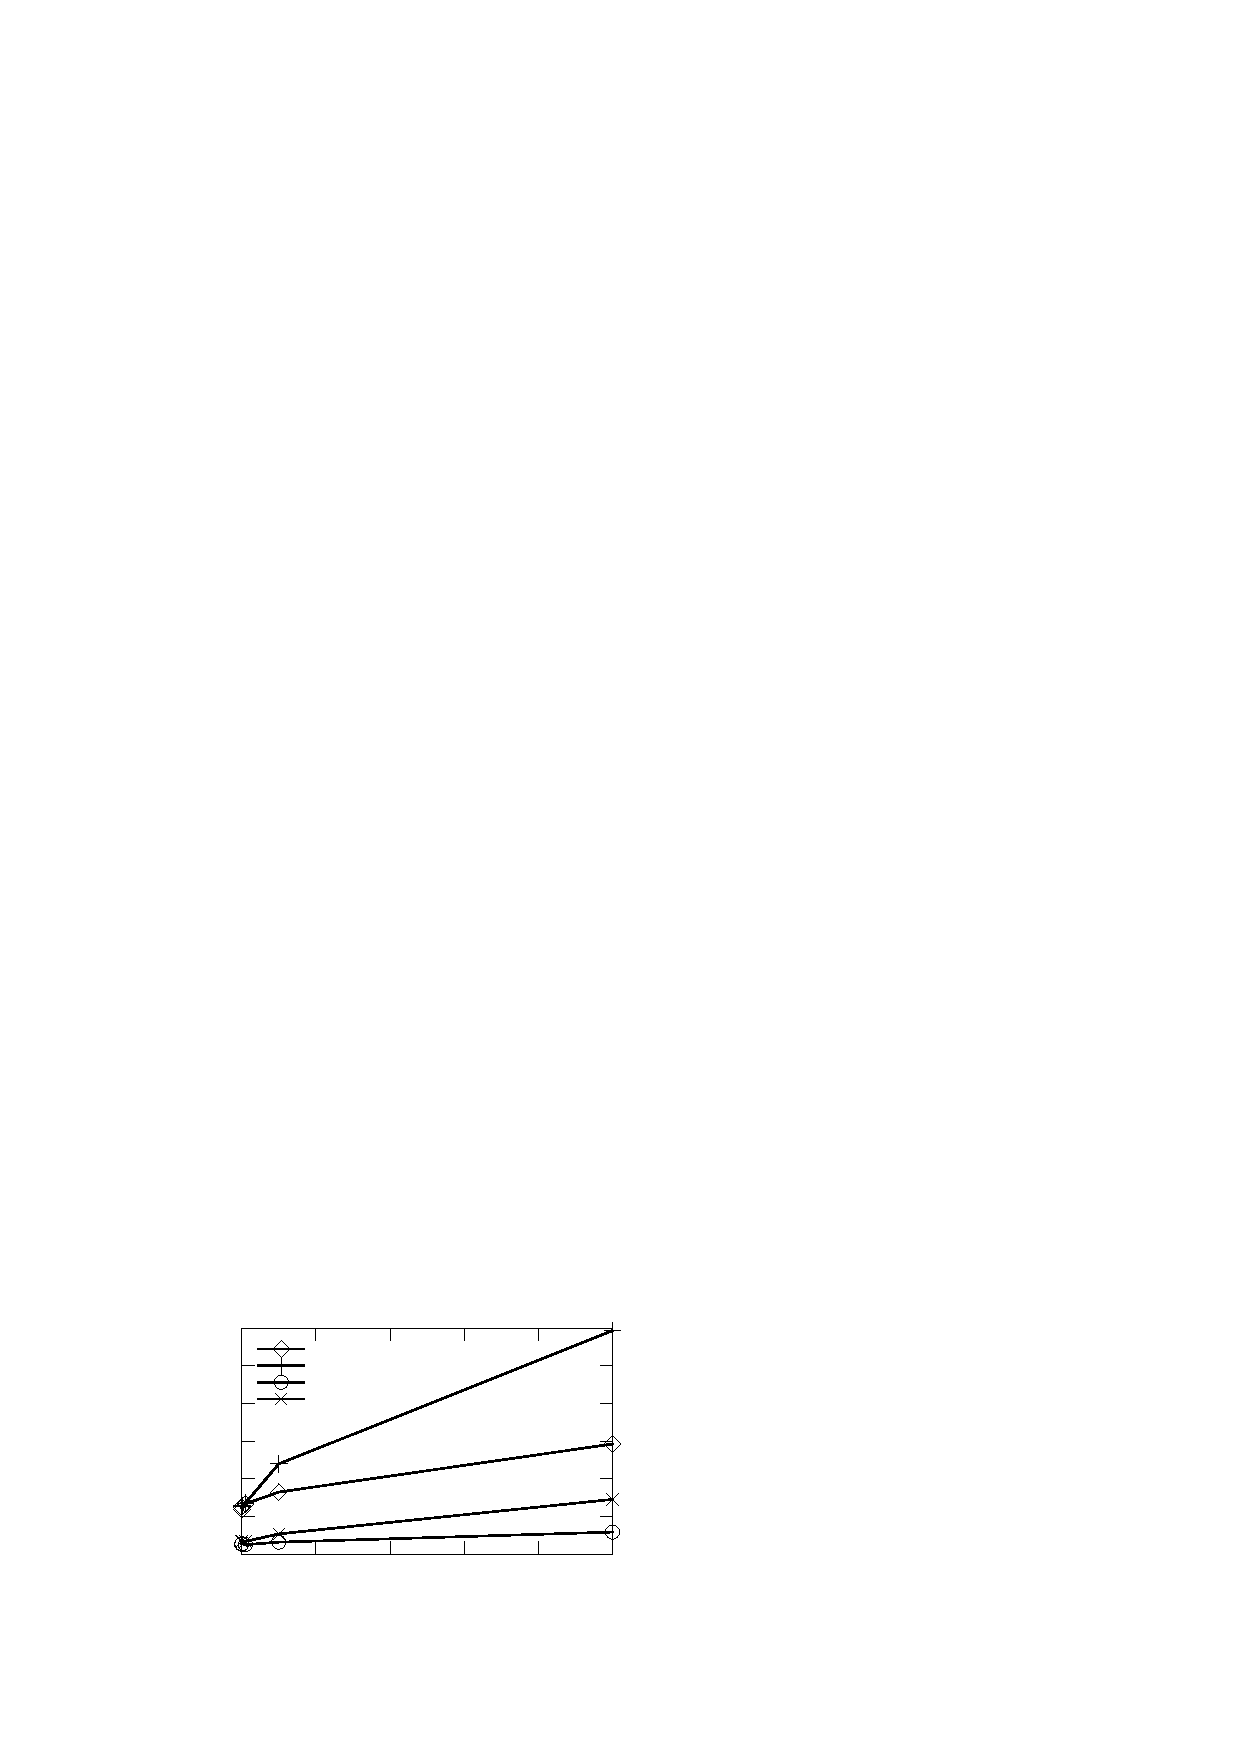
\includegraphics{stab_area}%
\end{picture}%
\begingroup
\setlength{\unitlength}{0.0200bp}%
\begin{picture}(11699,7019)(0,0)%
\put(2000,1200){\makebox(0,0)[r]{\strut{} 0}}%
\put(2000,2103){\makebox(0,0)[r]{\strut{} 2000}}%
\put(2000,3007){\makebox(0,0)[r]{\strut{} 4000}}%
\put(2000,3910){\makebox(0,0)[r]{\strut{} 6000}}%
\put(2000,4813){\makebox(0,0)[r]{\strut{} 8000}}%
\put(2000,5717){\makebox(0,0)[r]{\strut{} 10000}}%
\put(2000,6620){\makebox(0,0)[r]{\strut{} 12000}}%
\put(2200,800){\makebox(0,0){\strut{} 0}}%
\put(3980,800){\makebox(0,0){\strut{} 2}}%
\put(5760,800){\makebox(0,0){\strut{} 4}}%
\put(7540,800){\makebox(0,0){\strut{} 6}}%
\put(9320,800){\makebox(0,0){\strut{} 8}}%
\put(11100,800){\makebox(0,0){\strut{} 10}}%
\put(400,3910){\rotatebox{90}{\makebox(0,0){Time [$\mu s$]}}}%
\put(6650,200){\makebox(0,0){Window Query Area [\%]}}%
\put(3900,6120){\makebox(0,0)[l]{\strut{}DCT-16K}}%
\put(3900,5720){\makebox(0,0)[l]{\strut{}RTREE-16K}}%
\put(3900,5320){\makebox(0,0)[l]{\strut{}DCT-4K}}%
\put(3900,4920){\makebox(0,0)[l]{\strut{}RTREE-4K}}%
\end{picture}%
\endgroup
\endinput
}
    \label{fig:stab_area}
  }
  \subfigure[Query times vs. aspect ratio of stream]{
    \scalebox{0.85}{%GNUPLOT: LaTeX picture with Postscript
\begin{picture}(0,0)%
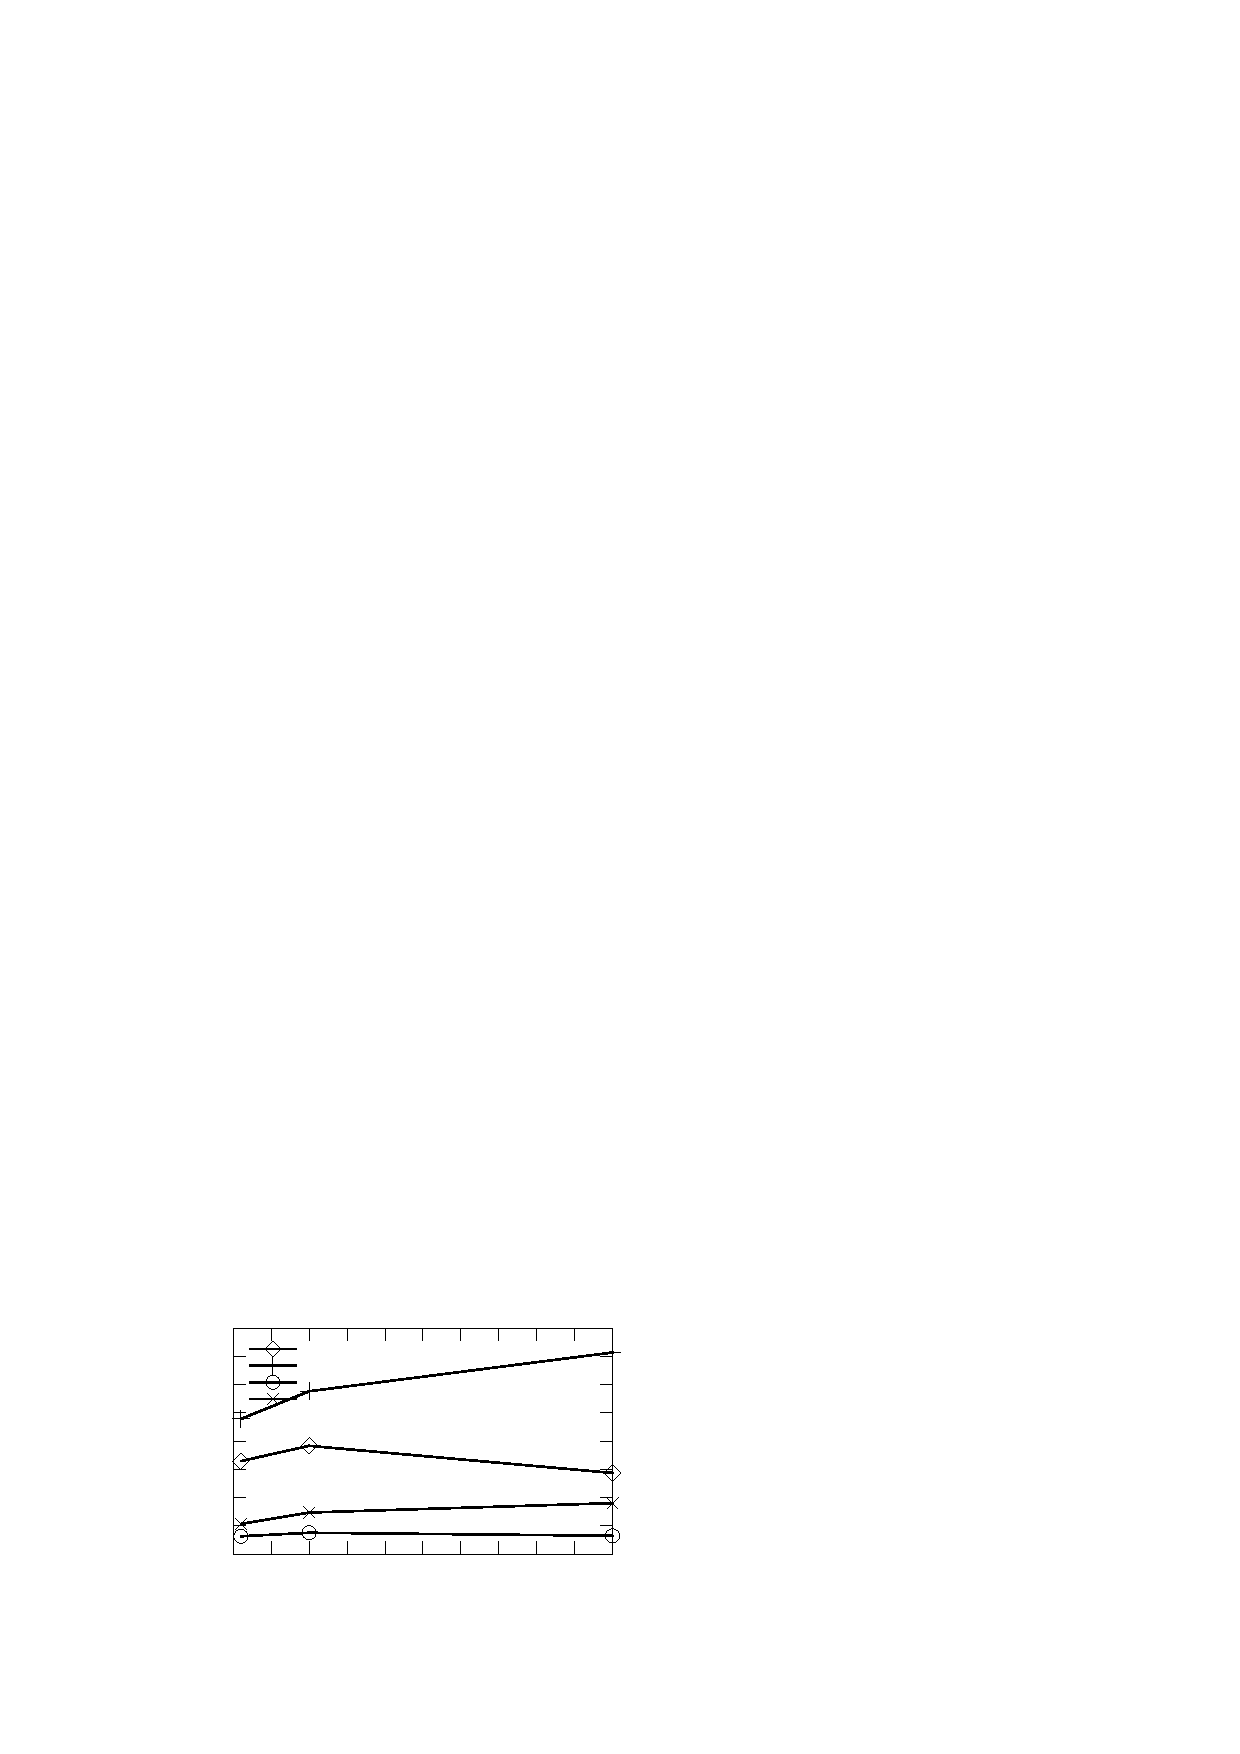
\includegraphics{stab_aspect}%
\end{picture}%
\begingroup
\setlength{\unitlength}{0.0200bp}%
\begin{picture}(11699,7019)(0,0)%
\put(1800,1200){\makebox(0,0)[r]{\strut{} 0}}%
\put(1800,1877){\makebox(0,0)[r]{\strut{} 1000}}%
\put(1800,2555){\makebox(0,0)[r]{\strut{} 2000}}%
\put(1800,3232){\makebox(0,0)[r]{\strut{} 3000}}%
\put(1800,3910){\makebox(0,0)[r]{\strut{} 4000}}%
\put(1800,4587){\makebox(0,0)[r]{\strut{} 5000}}%
\put(1800,5265){\makebox(0,0)[r]{\strut{} 6000}}%
\put(1800,5942){\makebox(0,0)[r]{\strut{} 7000}}%
\put(1800,6620){\makebox(0,0)[r]{\strut{} 8000}}%
\put(2000,800){\makebox(0,0){\strut{} 0}}%
\put(2910,800){\makebox(0,0){\strut{} 5}}%
\put(3820,800){\makebox(0,0){\strut{} 10}}%
\put(4730,800){\makebox(0,0){\strut{} 15}}%
\put(5640,800){\makebox(0,0){\strut{} 20}}%
\put(6550,800){\makebox(0,0){\strut{} 25}}%
\put(7460,800){\makebox(0,0){\strut{} 30}}%
\put(8370,800){\makebox(0,0){\strut{} 35}}%
\put(9280,800){\makebox(0,0){\strut{} 40}}%
\put(10190,800){\makebox(0,0){\strut{} 45}}%
\put(11100,800){\makebox(0,0){\strut{} 50}}%
\put(400,3910){\rotatebox{90}{\makebox(0,0){Time [$\mu s$]}}}%
\put(6550,200){\makebox(0,0){Window Query Aspect [$\frac{x}{y}$]}}%
\put(3700,6120){\makebox(0,0)[l]{\strut{}DCT-16K}}%
\put(3700,5720){\makebox(0,0)[l]{\strut{}RTREE-16K}}%
\put(3700,5320){\makebox(0,0)[l]{\strut{}DCT-4K}}%
\put(3700,4920){\makebox(0,0)[l]{\strut{}RTREE-4K}}%
\end{picture}%
\endgroup
\endinput
}
    \label{fig:stab_aspect}
  }
  \caption{Area and aspect tests}
\end{figure}


Figure~\ref{fig:stab_aspect}
shows the change in response time as a function of aspect ratio.  The
R*-tree performance is slightly degraded as the aspect ratio
increases, while the \ac{DCT} performance remains insensitive to this
parameter.


Section~\ref{sec:performance} described how the \ac{DCT} can be affected
by the average trajectory of the successive data from the stream.
Performance is expected to improve as window trajectory aligns with
the dimensions farther down in the \ac{DCT} cascade.
Figure~\ref{fig:dir} illustrates this gain.  As expected, the R*-tree
is insensitive to this parameter, whereas the \ac{DCT}'s performance
increases by a factor of two based on the trajectory of the query
window.

Figure~\ref{fig:area} shows the affect of the average size of the
\ac{CQ} \acp{ROI} on the \ac{DCT} performance.  As the size of the \acp{ROI}
increases, the average response time increases for both search
structures, due in part to the fact that more \acp{ROI} overlap with
each individual window query.

\begin{figure}[htb]
  \subfigure[Query times vs. trajectory of window]{ 
    \scalebox{0.85}{%GNUPLOT: LaTeX picture with Postscript
\begin{picture}(0,0)%
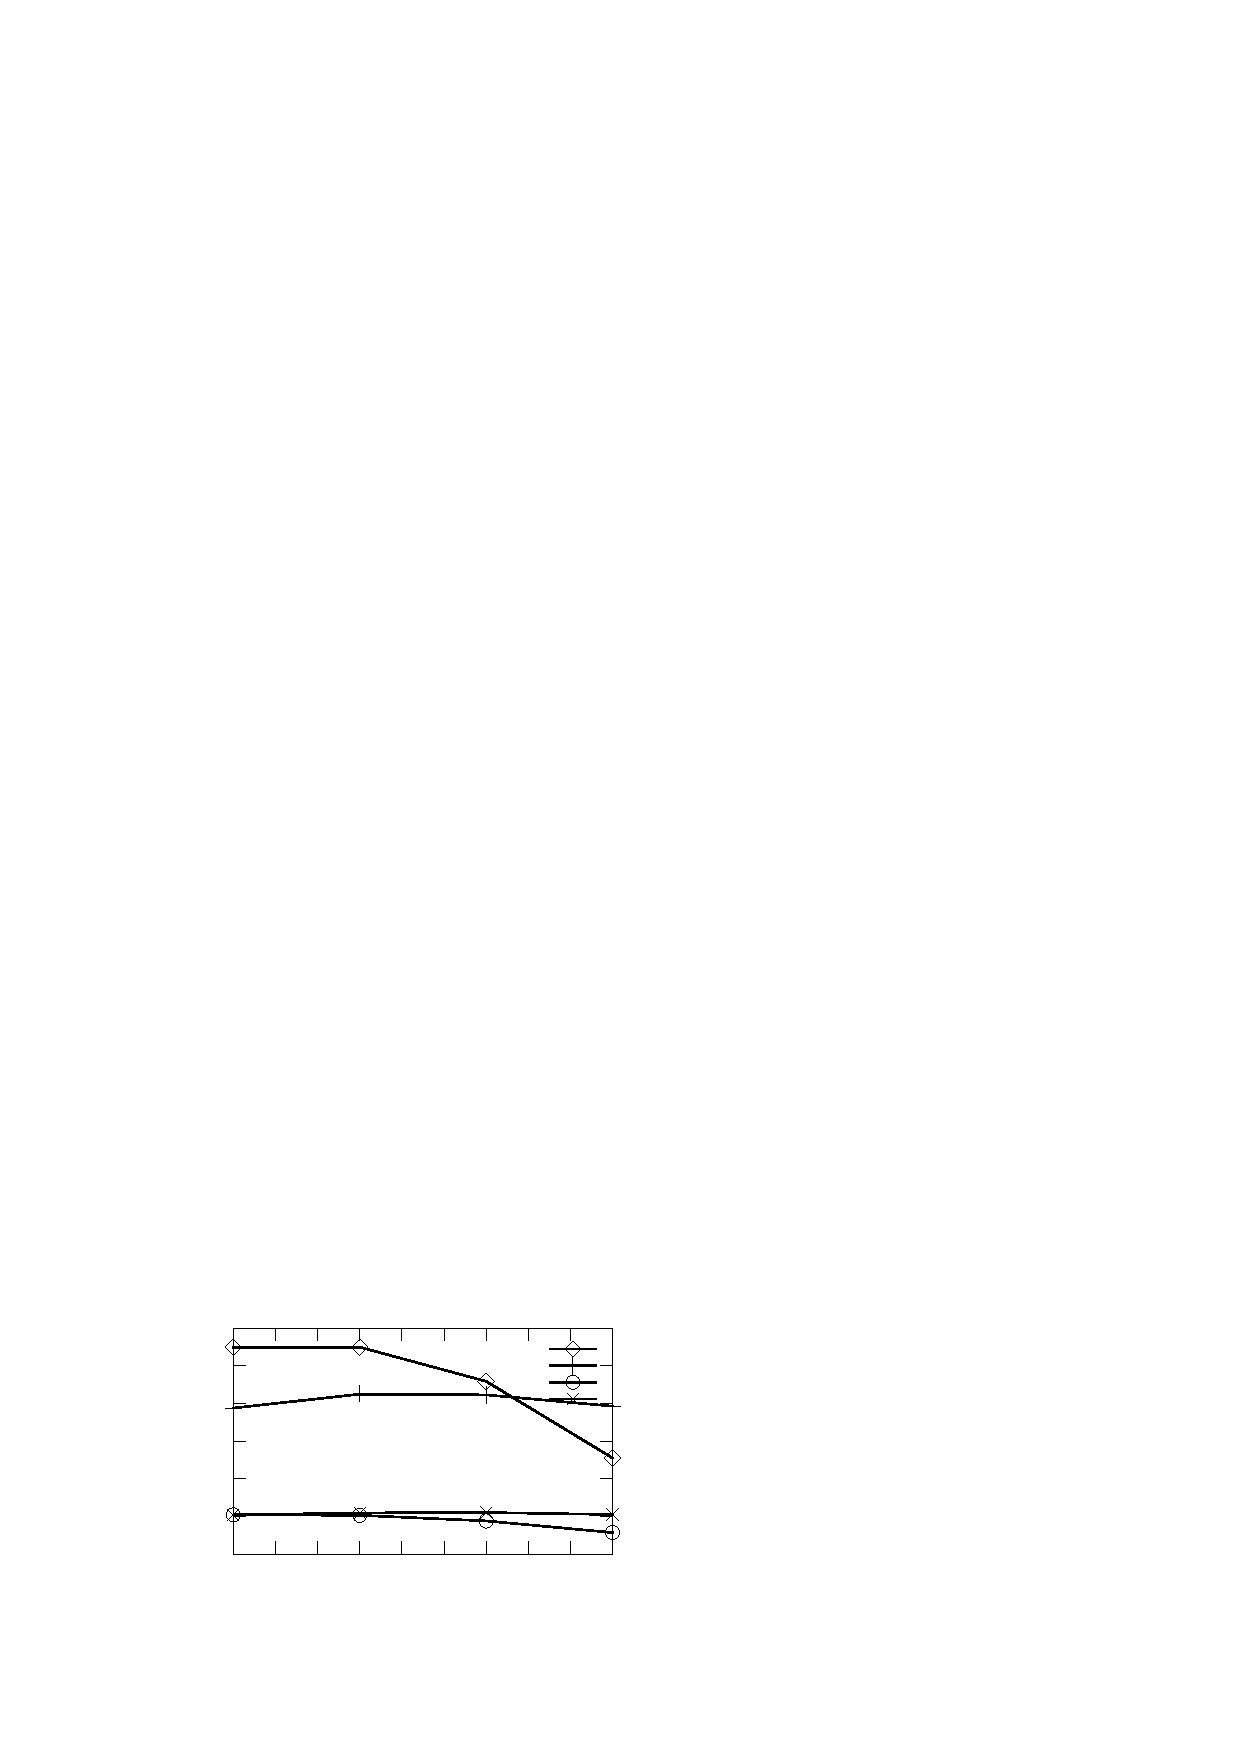
\includegraphics{dir}%
\end{picture}%
\begingroup
\setlength{\unitlength}{0.0200bp}%
\begin{picture}(11699,7019)(0,0)%
\put(1800,1200){\makebox(0,0)[r]{\strut{} 0}}%
\put(1800,2103){\makebox(0,0)[r]{\strut{} 1000}}%
\put(1800,3007){\makebox(0,0)[r]{\strut{} 2000}}%
\put(1800,3910){\makebox(0,0)[r]{\strut{} 3000}}%
\put(1800,4813){\makebox(0,0)[r]{\strut{} 4000}}%
\put(1800,5717){\makebox(0,0)[r]{\strut{} 5000}}%
\put(1800,6620){\makebox(0,0)[r]{\strut{} 6000}}%
\put(2000,800){\makebox(0,0){\strut{} 0}}%
\put(3011,800){\makebox(0,0){\strut{} 10}}%
\put(4022,800){\makebox(0,0){\strut{} 20}}%
\put(5033,800){\makebox(0,0){\strut{} 30}}%
\put(6044,800){\makebox(0,0){\strut{} 40}}%
\put(7056,800){\makebox(0,0){\strut{} 50}}%
\put(8067,800){\makebox(0,0){\strut{} 60}}%
\put(9078,800){\makebox(0,0){\strut{} 70}}%
\put(10089,800){\makebox(0,0){\strut{} 80}}%
\put(11100,800){\makebox(0,0){\strut{} 90}}%
\put(400,3910){\rotatebox{90}{\makebox(0,0){Time [$\mu s$]}}}%
\put(6550,200){\makebox(0,0){Trajectory Direction [deg]}}%
\put(9400,6120){\makebox(0,0)[r]{\strut{}DCT-16K}}%
\put(9400,5720){\makebox(0,0)[r]{\strut{}RTREE-16K}}%
\put(9400,5320){\makebox(0,0)[r]{\strut{}DCT-4K}}%
\put(9400,4920){\makebox(0,0)[r]{\strut{}RTREE-4K}}%
\end{picture}%
\endgroup
\endinput
}
    \label{fig:dir}
  }
  \subfigure[Query times vs \ac{ROI} area]{
      \scalebox{0.85}{%GNUPLOT: LaTeX picture with Postscript
\begin{picture}(0,0)%
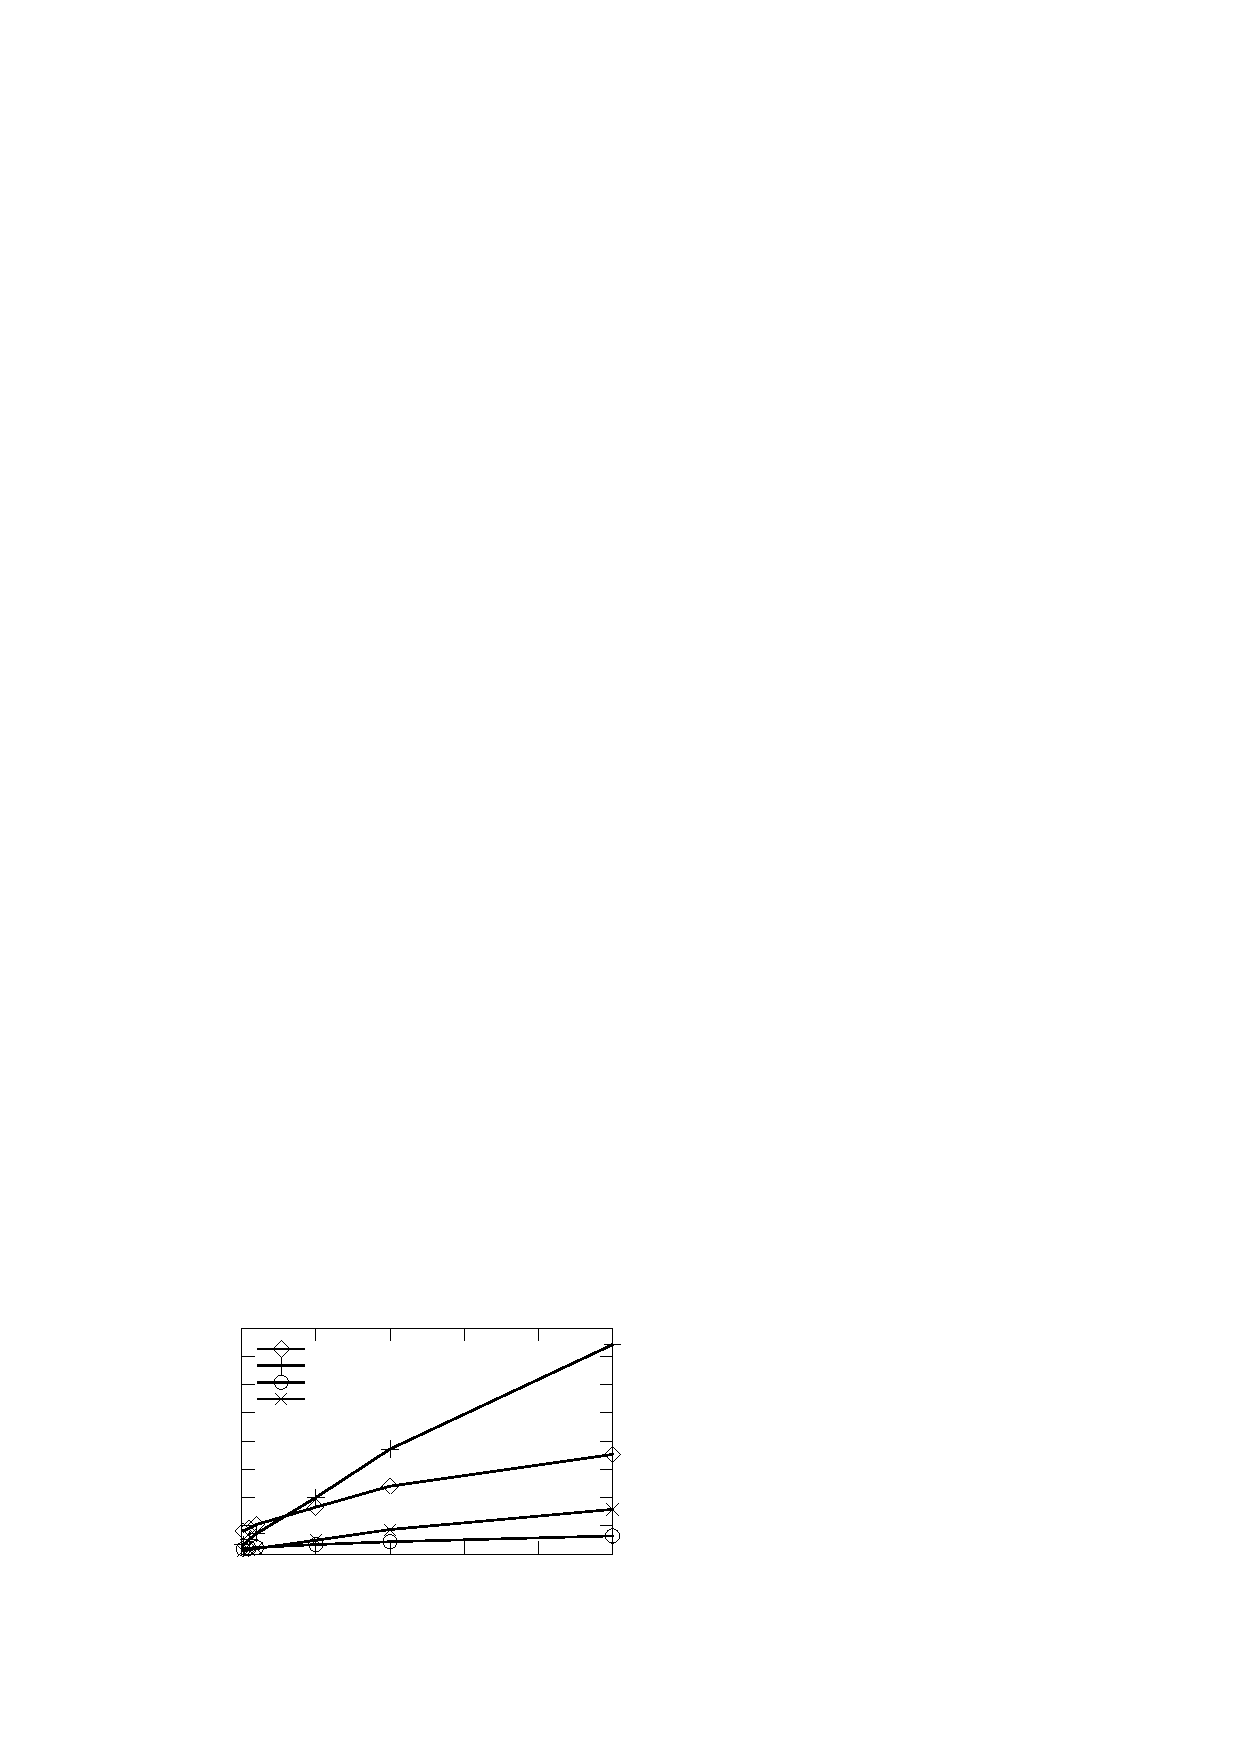
\includegraphics{area}%
\end{picture}%
\begingroup
\setlength{\unitlength}{0.0200bp}%
\begin{picture}(11699,7019)(0,0)%
\put(2000,1200){\makebox(0,0)[r]{\strut{} 0}}%
\put(2000,1877){\makebox(0,0)[r]{\strut{} 2000}}%
\put(2000,2555){\makebox(0,0)[r]{\strut{} 4000}}%
\put(2000,3232){\makebox(0,0)[r]{\strut{} 6000}}%
\put(2000,3910){\makebox(0,0)[r]{\strut{} 8000}}%
\put(2000,4587){\makebox(0,0)[r]{\strut{} 10000}}%
\put(2000,5265){\makebox(0,0)[r]{\strut{} 12000}}%
\put(2000,5942){\makebox(0,0)[r]{\strut{} 14000}}%
\put(2000,6620){\makebox(0,0)[r]{\strut{} 16000}}%
\put(2200,800){\makebox(0,0){\strut{} 0}}%
\put(3980,800){\makebox(0,0){\strut{} 5}}%
\put(5760,800){\makebox(0,0){\strut{} 10}}%
\put(7540,800){\makebox(0,0){\strut{} 15}}%
\put(9320,800){\makebox(0,0){\strut{} 20}}%
\put(11100,800){\makebox(0,0){\strut{} 25}}%
\put(400,3910){\rotatebox{90}{\makebox(0,0){Time [$\mu s$]}}}%
\put(6650,200){\makebox(0,0){Input Area [\%]}}%
\put(3900,6120){\makebox(0,0)[l]{\strut{}DCT-16K}}%
\put(3900,5720){\makebox(0,0)[l]{\strut{}RTREE-16K}}%
\put(3900,5320){\makebox(0,0)[l]{\strut{}DCT-4K}}%
\put(3900,4920){\makebox(0,0)[l]{\strut{}RTREE-4K}}%
\end{picture}%
\endgroup
\endinput
}
      \label{fig:area}
    }
    \caption{Trajectory and \ac{ROI} experiments}
\end{figure}

The R*-tree slows down more than the \ac{DCT}, since more of the results
from successive window queries can be shared from query to query.
This is an important consideration for applications where the \ac{CQ}
\acp{ROI} are large.

In summary, the \ac{DCT} performance is affected by the number of \ac{ROI}
boundaries crossed for successive window queries, and the trajectory
of the window queries. Also the size of the \ac{CQ} \acp{ROI} and input
data extents affect performance.  Often the performance changes are
different than seen in the more typical R*-tree.  How the \ac{DCT}
performs under more realistic situations is described next.

\subsection{GOES Experiment}
\label{sec:goesex}

From the discussion of the \ac{DCT} performance and the experimental
results for random windows and \acp{ROI}, the parameters associated with
higher performance of the \ac{DCT} can be anticipated.  These include:
(1) relatively large extents of data in the stream, possibly with a
high aspect ratio, (2) small distances from data to data in the
stream, and (3) a regular trajectory of the data in the stream, with
the \ac{DCT} tuned to that direction.  The \ac{DCT} also works well with
large \ac{CQ} \acp{ROI}, having a relatively high selectivity.  These
are all aspects of a typical satellite \ac{RSI} data stream.

For a more realistic scenario for the \ac{DCT}, an experiment using
queries for weather satellite data, from \ac{NOAA} \ac{GOES} was
developed.  Figure~\ref{tab:goes} (page~\pageref{tab:goes}), included
an overview of the \ac{GOES} sensors.  The experiment uses Imager data
as input.  \ac{GOES} offers a continuous stream of data for \acp{ROI}
ranging from the continental United States to a hemisphere centered
near Hawaii.  Query regions also tend to be approximately square
regions covering relatively large extents.

\ac{GOES} streaming \ac{RSI} data is well suited to the \ac{DCT}.  In each
frame, the data trends only in the downward direction and
incrementally.  Therefore, endpoints are only added into the \Xn, \Xx\ 
structures one time, limiting the maintenance time to $O(n\lg{n})$ for
each frame.  For normal \ac{GOES} data, the starting column of each
row does not change within a frame and the \Yn, \Yx\ and \id{A} 
structures are the only structures that change in determining which
\acp{ROI} overlap any given set of incoming streaming rows of data.

For the experiment, five thousand (5,000) \acp{ROI} were indexed.
Rather than randomly locate these \acp{ROI} throughout the image domain,
they were preferentially located around a small number of ``hot
spots'' in the hemisphere.  This more closely relates to real world
scenarios, where specific parts of the \ac{RSI} data is requested by
a large numbers of users.  Although the general area of the queries
was fixed to a small number of locations, the individual \ac{ROI}
centers, total sizes and aspect ratios were varied for each \ac{ROI}.
This corresponds to many users requesting slightly different
particulars for a general \ac{ROI}.  A small fraction of
random \acp{ROI} was also included in the experimental setup.
Table~\ref{tab:goes-ex} describes the parameters for the \ac{CQ}
\acp{ROI}.  The contributions table shows the various general regions
and their contributions to the total \acp{ROI}.  The other table shows
the variation of the individual \acp{ROI}.  The figure graphically
depicts the experimental setup.

\begin{table}[htb]
  \centering
  \caption{Query \ac{ROI} statistics}
  \begin{tabular}[t]{cl||cl}
    \multicolumn{2}{c|}{Contributions} & \multicolumn{2}{|c}{\ac{ROI} Variations} \\
    \hline \hline
    $30\%$ & North America & Area & 0.8-1.2 \\
    $15\%$ & Western Seaboard & Aspect & $\pm 10\%$ \\
    $15\%$ & Northern Hemisphere & Center & $\pm 10\%$ \\
    $15\%$ & Hemisphere & \multicolumn{2}{|c}{\multirow{5}{4cm}{\centering 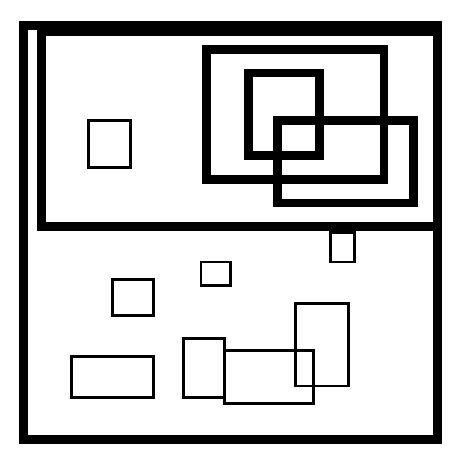
\includegraphics[width=3cm]{figs/performance-goes.fig.eps}}}         \\     
    $9\%$  & CA  &           \\    
    $9\%$ & Mexico &             \\    
    $2\%$ & Random (1000x1000) &  \\    
    $5\%$ & Random (6000x4000) &       \\
  \end{tabular}
  \label{tab:goes-ex}
\end{table}

Ten thousand (10,000) window queries were performed on the \ac{CQ}
\acp{ROI}.  The \ac{RSI} data blocks corresponding to the input data
stream were taken from a sample of the \ac{GOES} West Imager
instrument, each query corresponding to 8 rows of data.  Depending on
some assumptions about other aspects of a \ac{DSMS} indexing \ac{GOES}
data, this corresponds to somewhere between 7.5 to 60 minutes of
streaming time.

Again, the \ac{DCT} was compared to the in-memory R*-tree implementation.
The R*-tree implementation required 48 seconds to perform all the
queries, for an average query time of 4800 [$\mu s$].  The \ac{DCT}
performed the queries in 9 seconds, 900 [$\mu s$] per query.  It is
also interesting to note that of those nine seconds for the \ac{DCT}, only
0.88 seconds where used in the maintenance of the \ac{DCT} and its
structures.  Nearly all the other 8.22 seconds involved copying the
final result \id{A} structure into new lists for output.  This was done to
match the output of the R*-tree, but scenarios can be envisioned where
applications access the \id{A} structure directly after a query, reducing
this overhead cost.

With respect to \ac{GOES} data, the reason for extending the structure
to account for more general trending data has to do with projection
systems.  Like most remotely sensed imagery, the original data is in
it is own projection system, while users would like to have data
streamed in a projection system of their choice, \ac{UTM} for example.
Re-projection is an expensive operation that should be avoided for
data not answering a specific query.  Allowing users to
specify queries in their projection system requires have a number of
\ac{DCT} structures, one for each input projection system.  All query
\acp{ROI} will be projected into the \ac{GOES} system, and roughly
described with a bounding box.  For each projection included with a
\ac{ROI} identified in this first \ac{DCT} structure, the bounding box of
the incoming rows of \ac{GOES} data will be re-projected into that
system, and represented with a new bounding box.  This box will be
used to identify the final intersections of the incoming \ac{GOES}
stream with the \acp{ROI}.  In those other projection
schemes, the incoming rows will still trend in a smooth line, but in
both $x$ and $y$ coordinates.


%%%%%%%%%%%%%%%%%%%%%%%%%%%%%%%%%%%%%%%%%%%%%%%%%%%%%%%%%%%%%%%%%%%%%%
%%%%%%%%%%%%%%%%%%%%%%%%%%%%%%%%%%%%%%%%%%%%%%%%%%%%%%%%%%%%%%%%%%%%%%
%%%%%%%%%%%%%%%%%%%%%%%%%%%%%%%%%%%%%%%%%%%%%%%%%%%%%%%%%%%%%%%%%%%%%%
\section{Temporal Dimension}
\label{sec:temporal}

Th focus for both the discussion and the experiments has so far been
on the spatial dimensions.  This is primarily because the \ac{DCT} takes
most advantage of the spatial organization of the incoming \ac{RSI}
data stream.  As has been discussed, adding additional dimensions is a
simple extension of another intermediate set of endpoint trees added
to the cascade in the \ac{DCT}.  The most obvious choice for another
dimension is the temporal domain, since most restrictions in user
queries include a temporal restriction as well.

\begin{figure}[htb]
  \centering
  \begin{picture}(0,0)%
\includegraphics{figs/temporal.fig.eps}%
\end{picture}%
\setlength{\unitlength}{4144sp}%
%
\begingroup\makeatletter\ifx\SetFigFont\undefined%
\gdef\SetFigFont#1#2#3#4#5{%
  \reset@font\fontsize{#1}{#2pt}%
  \fontfamily{#3}\fontseries{#4}\fontshape{#5}%
  \selectfont}%
\fi\endgroup%
\begin{picture}(6649,3140)(69,-2288)
\put(4276,-1996){\makebox(0,0)[lb]{\smash{{\SetFigFont{10}{12.0}{\rmdefault}{\mddefault}{\updefault}{\color[rgb]{0,0,0}Time}%
}}}}
\put(2251,-2086){\makebox(0,0)[lb]{\smash{{\SetFigFont{8}{9.6}{\familydefault}{\mddefault}{\updefault}{\color[rgb]{0,0,0}Cascade to $x$}%
}}}}
\put(4726,-511){\makebox(0,0)[lb]{\smash{{\SetFigFont{8}{9.6}{\familydefault}{\mddefault}{\updefault}{\color[rgb]{0,0,0}\wt}%
}}}}
\put(6211,389){\makebox(0,0)[lb]{\smash{{\SetFigFont{11}{13.2}{\familydefault}{\mddefault}{\updefault}{\color[rgb]{0,0,0}\Tx}%
}}}}
\put(5536,-241){\makebox(0,0)[lb]{\smash{{\SetFigFont{8}{9.6}{\familydefault}{\mddefault}{\updefault}{\color[rgb]{0,0,0}\wt}%
}}}}
\put(3961,344){\makebox(0,0)[lb]{\smash{{\SetFigFont{11}{13.2}{\familydefault}{\mddefault}{\updefault}{\color[rgb]{0,0,0}\Tn}%
}}}}
\put(3466,-241){\makebox(0,0)[lb]{\smash{{\SetFigFont{8}{9.6}{\familydefault}{\mddefault}{\updefault}{\color[rgb]{0,0,0}\wt}%
}}}}
\end{picture}%

  \caption[\ac{DCT} temporal dimension]{%
    Temporal dimension added to the \ac{DCT}.  Shown
    are region's temporal extents, the endpoint trees \Tn\ and \Tx,
    and the temporal node pointer, \wt.}
  \label{fig:temporal}
\end{figure}

Figure~\ref{fig:temporal} shows an extension of the \ac{DCT} in the
temporal domain.  Here, time is the first dimension of the cascade.
As discussed in Section~\ref{sec:performance}, it is best to order the
dimensions so the most varying is on the deeper levels of the \ac{DCT}.
For relatively low bandwidth pixel-by-pixel \ac{RSI} streams, the
monotonic increase of time would make it a candidate for the level
directly before the \id{A} tree.  However, for most \ac{RSI} data,
putting time as the first dimension makes most sense, because most of
the variation comes in the spatial domains.  

There are some features more specific to the temporal domain.  One
possibility is for unbounded regions, two of which, $a,f$, are shown
in the figure.  These correspond to \acp{CQ} without a
specified ending time.  Unbounded regions can be modeled in the \ac{DCT} 
by simply not including endpoints in the \Tx\ endpoint tree.  The
temporal domain is more likely to contain a discontinuous region, for
example, \ac{ROI} $c$ in the figure.  This corresponds to a periodic
query, for example, a request for the noon satellite image for a period
of days.  Although more problematic for \ac{CQ} extents,
discontinuities can generally be handled with multiple entries in the
\ac{DCT} endpoint trees.
 
One nice feature with making time the first structure of the cascade
is that it can also serve as providing a structure to prune \acp{ROI}
that have expired.  When \wt\ crosses over the maximum time endpoint
for any of the \ac{CQ} \acp{ROI}, the \ac{DCT} will cascade a deletion
through the remaining trees.  These \acp{ROI} can then also be removed
from the temporal endpoint trees as well, removing those \acp{ROI}
completely from the \ac{DCT}.  An interesting point to this is that \wt\
will always be pointing to the minimum node of the \Tx\ endpoint tree,
as finished \acp{ROI} are deleted.  Because of the monotonicity of time
for the incoming data stream, besides using the standard trees for the
temporal dimension, more efficient structures like heaps could be
investigated for this dimension.

\section{Non-spatial Multi-dimensional Data}
%
The focus of the \ac{DCT} has been on spatial data.  However, these
techniques could be applied to a general multi-dimensional data space.
The obvious modifications could be made and extended to $n$ dimensions
as outlined above.  One important issue to address is the order of the
cascade of \id{2KeyList} structures.  As described in
Section~\ref{sec:performance}, if \acp{ROI} are dispersed equally, it is
generally best to move the most varying parameter to the end of the
cascade, and move the least varying to the top.  This structure is
also appropriate for range queries over a single dimension over
trending data by maintaining only the top \id{2KeyList}.  Since the index
sizes are relatively small, it is conceivable that a system could
consistently maintain one dimensional \ac{DCT} structures, and then
dynamically begins to build 2 or $n$ dimensional structures when
queries requesting such \acp{ROI} are instantiated.  The advantage of
this method is that the structures are no longer maintained as the
queries requesting those \acp{ROI} are deleted.

\section{Related Work}
\label{sec:related}

The structure and performance characteristics of the \ac{DCT} have
previously been
described~\cite{hart04index-query,DBLP:conf/ssd/HartGZ05}.  The
primary goal of the \ac{DCT} is to allow for many spatial \acp{ROI} to
be simultaneously evaluated as the stream of input spatial data
arrives in the \ac{DSMS}.  The obvious application of the \ac{DCT} is
in multi-query evaluation, where a single operator uses the \ac{DCT}
structure to perform the spatial restrictions for a large number of
queries.

Similar multi-query optimizations have been discussed in streaming
databases where they have been described as group
filters~\cite{madden02fjord-stream, madden02contin-adapt} and in
spatio-temporal databases where this optimization has been described
as query indexing~\cite{prabhakar02qindex}.

Many data structures have been developed for one and two dimensional
stabbing and window queries including among others, interval trees,
priority search trees, and segment trees~\cite{berg00comput-geomet}.
Space partitioning methods of answering window queries include
quadtrees, hashes, and numerous variants of R-trees.

The common methods for solving window queries in two dimensions are
multi-level segment trees~\cite{berg00comput-geomet} and
R-trees~\cite{guttm84r-tree}.  It is difficult to modify either method
to take advantage of trending data.  Using multi-level segment trees,
one dimension of the \ac{ROI} is stored in a segment tree, while the
second dimension is indexed with an associated interval structure for
each node in the first segment tree.  Storage for these structures can
be $O(n\lg{n})$, with query times of $O(\lg^2{n})$.  Dynamic
maintenance of such a structure is more complicated and requires
larger storage costs~\cite{krevel88concat-segmen}.  It is difficult to
modify the multi-level segment tree to improve results for trending
data.  If the input window moves a small distance, which doesn't
change the query results, it still would take $O(\lg{n})$ time to
respond.  That is because even if every node in the multi-level
segment tree maintains knowledge of the previous point, it would still
take $\lg({n})$ time to traverse the primary segment tree would still
need to be traversed to discover that no changes to the query
occurred.

R-trees solve window queries by traversing through minimum bounding
rectangles that include the extent of all regions in the sub-tree,
generally with good performance.  Since these rectangle regions
generally overlap, there can be no savings from knowing the previous
window, as there is no way to know if an entirely new path through the
segment tree needs to be traversed.  R$^+$-trees~\cite{sellis87r-tree}
style trees may be modified for trending windows, since the minimum
bounding rectangles are not allowed to overlap and maintaining the
previous window can help verify a query hasn't left a particular
region.  R$^+$-trees, however, have problems with redundant storage,
dynamic updates, and potential deadlocks~\cite{manol03r-have}.

Another approach similar to the \ac{DCT} described in this chapter is that
of the query index~\cite{kalas04main-memor, prabhakar02qindex}.  The
query index builds a space partitioning index on a set of static query
\acp{ROI} and at each time interval, allows a number of moving objects
to probe the index to determine overlapping queries.  Experiments in
main memory implementations show that grid-based hashing of query
\acp{ROI} generally outperform R-tree or quad-tree based methods.  The
query index is most effective for small \acp{ROI} and query points, and
experiments show performance degradation with larger \acp{ROI} or high
selectivity query windows~\cite{kim01optim}.


All of these indexes described above anticipate a large number of
moving objects to be indexed against the query \acp{ROI}.  The \acs{RSI}
application described above is different in the sense that the \ac{DCT}
index is designed for a single or small number of moving objects,
where the input rate of data for that moving object is very large.  In
this application, the desire is for a small index that can efficiently
route that high volume data stream to the query regions, rather than
indexes that are interested in the location of the moving objects.

The \ac{DCT} is also an incremental approach to answering queries, where
updates are made to a current query result.  SINA~\cite{mokbel04sina},
describes an incremental method to solving the problem intersecting
moving objects, though the approach focuses on efficient integration
of incremental query changes with disk-based static queries, and a
complete main-memory implementation would be more similar to the query
index approach.

In another sense, the \ac{DCT} is a method of dynamically maintaining
boundaries around a current window where the current result set is
valid and identifying where this result set will change.  Another
method of dynamically describing a neighborhood of validity for a
query using R-trees was proposed in~\cite{zhang03locat},
 which builds an explicit region of validity around a current query
point.  This method is meant to minimize transmission costs to a
client, and the technique makes many additional queries to an R-tree
style index to build these regions of validity.


\chapter{Multi-Query Execution Using an Online System}
\label{cha:operators}


Chapter~\ref{cha:existing} described a multi-query optimization system
using an existing \ac{GIS} application.  While this system is
promising in its approach, a \ac{DSMS} system designed specifically
for \ac{RSI} data would behave differently, operating on smaller
discrete parts of an image directly as \ac{RSI} data arrive.  This
chapter will provide more detailed information on the various
components of an online \ac{DSMS}.  It is meant as a high level
implementation design.  The focus of the discussion will be on the
requirements particular to the processing of the \ac{GOES} \ac{GVAR}
data.

The data from the stream will be a manipulated a single row at a time.
This is most consistent with the data stream arrival pattern and will
allow for the smallest in-memory footprint of the system as a whole.
In addition, as was discussed in Section~\ref{sec:point-sets}
(page~\pageref{sec:point-sets}), row-scan ordering allows for
processing benefits especially in the presence of image restrictions.
Figure~\ref{fig:overview} (page~\pageref{fig:overview}) described an
overview of the \ac{GS} architecture.
Figure~\ref{fig:overview-detail} revisits this overview in more
detail.
%
\begin{figure}[htb]
  \centering
  \scalebox{0.7}{\begin{picture}(0,0)%
\includegraphics{figs/overview-detail.fig.eps}%
\end{picture}%
\setlength{\unitlength}{3947sp}%
%
\begingroup\makeatletter\ifx\SetFigFontNFSS\undefined%
\gdef\SetFigFontNFSS#1#2#3#4#5{%
  \reset@font\fontsize{#1}{#2pt}%
  \fontfamily{#3}\fontseries{#4}\fontshape{#5}%
  \selectfont}%
\fi\endgroup%
\begin{picture}(6924,10766)(2089,-10123)
\put(6413,-2888){\makebox(0,0)[b]{\smash{{\SetFigFontNFSS{12}{14.4}{\familydefault}{\mddefault}{\updefault}{\color[rgb]{0,0,0}\ac{GVAR} Input}%
}}}}
\put(3355,135){\makebox(0,0)[lb]{\smash{{\SetFigFontNFSS{5}{6.0}{\familydefault}{\mddefault}{\updefault}{\color[rgb]{0,0,0}connect}%
}}}}
\put(6213,-645){\makebox(0,0)[lb]{\smash{{\SetFigFontNFSS{6}{7.2}{\familydefault}{\mddefault}{\updefault}{\color[rgb]{0,0,0}Stream}%
}}}}
\put(6213,-786){\makebox(0,0)[lb]{\smash{{\SetFigFontNFSS{6}{7.2}{\familydefault}{\mddefault}{\updefault}{\color[rgb]{0,0,0}Generator}%
}}}}
\put(3355,-526){\makebox(0,0)[lb]{\smash{{\SetFigFontNFSS{5}{6.0}{\familydefault}{\mddefault}{\updefault}{\color[rgb]{0,0,0}connect}%
}}}}
\put(3355,-1140){\makebox(0,0)[lb]{\smash{{\SetFigFontNFSS{5}{6.0}{\familydefault}{\mddefault}{\updefault}{\color[rgb]{0,0,0}connect}%
}}}}
\put(4914,-408){\rotatebox{270.0}{\makebox(0,0)[lb]{\smash{{\SetFigFontNFSS{6}{7.2}{\familydefault}{\mddefault}{\updefault}{\color[rgb]{0,0,0}Parser}%
}}}}}
\put(5528,-408){\makebox(0,0)[lb]{\smash{{\SetFigFontNFSS{6}{7.2}{\familydefault}{\mddefault}{\updefault}{\color[rgb]{0,0,0}Optimization}%
}}}}
\put(4914,-928){\rotatebox{270.0}{\makebox(0,0)[lb]{\smash{{\SetFigFontNFSS{6}{7.2}{\familydefault}{\mddefault}{\updefault}{\color[rgb]{0,0,0}Delivery}%
}}}}}
\put(4772,-172){\makebox(0,0)[lb]{\smash{{\SetFigFontNFSS{6}{7.2}{\familydefault}{\mddefault}{\updefault}{\color[rgb]{0,0,0}\acs{DSMS} Server}%
}}}}
\put(8326,-8236){\makebox(0,0)[b]{\smash{{\SetFigFontNFSS{12}{14.4}{\familydefault}{\mddefault}{\updefault}{\color[rgb]{0,0,0}Queries}%
}}}}
\put(3413,-2888){\makebox(0,0)[b]{\smash{{\SetFigFontNFSS{12}{14.4}{\familydefault}{\mddefault}{\updefault}{\color[rgb]{0,0,0}Row Memory}%
}}}}
\put(4699,-5895){\makebox(0,0)[lb]{\smash{{\SetFigFontNFSS{12}{14.4}{\rmdefault}{\mddefault}{\updefault}{\color[rgb]{0,0,0}$f()$}%
}}}}
\put(4699,-4392){\makebox(0,0)[lb]{\smash{{\SetFigFontNFSS{12}{14.4}{\rmdefault}{\mddefault}{\updefault}{\color[rgb]{0,0,0}/ 2}%
}}}}
\put(5855,-4355){\makebox(0,0)[lb]{\smash{{\SetFigFontNFSS{12}{14.4}{\rmdefault}{\mddefault}{\updefault}{\color[rgb]{0,0,0}/ 2}%
}}}}
\put(7053,-4355){\makebox(0,0)[lb]{\smash{{\SetFigFontNFSS{12}{14.4}{\rmdefault}{\mddefault}{\updefault}{\color[rgb]{0,0,0}/ 2}%
}}}}
\put(3541,-4418){\makebox(0,0)[lb]{\smash{{\SetFigFontNFSS{12}{14.4}{\rmdefault}{\mddefault}{\updefault}{\color[rgb]{0,0,0}C1}%
}}}}
\put(7053,-5032){\makebox(0,0)[lb]{\smash{{\SetFigFontNFSS{12}{14.4}{\rmdefault}{\mddefault}{\updefault}{\color[rgb]{0,0,0}/ 2}%
}}}}
\put(5855,-5032){\makebox(0,0)[lb]{\smash{{\SetFigFontNFSS{12}{14.4}{\rmdefault}{\mddefault}{\updefault}{\color[rgb]{0,0,0}/ 2}%
}}}}
\put(4716,-5032){\makebox(0,0)[lb]{\smash{{\SetFigFontNFSS{12}{14.4}{\rmdefault}{\mddefault}{\updefault}{\color[rgb]{0,0,0}C2}%
}}}}
\put(4716,-8318){\makebox(0,0)[lb]{\smash{{\SetFigFontNFSS{12}{14.4}{\rmdefault}{\mddefault}{\updefault}{\color[rgb]{0,0,0}Q2}%
}}}}
\put(5303,-8318){\makebox(0,0)[lb]{\smash{{\SetFigFontNFSS{12}{14.4}{\rmdefault}{\mddefault}{\updefault}{\color[rgb]{0,0,0}Q3}%
}}}}
\put(4103,-8318){\makebox(0,0)[lb]{\smash{{\SetFigFontNFSS{12}{14.4}{\rmdefault}{\mddefault}{\updefault}{\color[rgb]{0,0,0}Q1}%
}}}}
\put(4716,-7092){\makebox(0,0)[lb]{\smash{{\SetFigFontNFSS{12}{14.4}{\familydefault}{\mddefault}{\updefault}{\color[rgb]{0,0,0}$\circ LL$}%
}}}}
\put(4216,-4411){\makebox(0,0)[lb]{\smash{{\SetFigFontNFSS{12}{14.4}{\familydefault}{\mddefault}{\updefault}{\color[rgb]{0,0,0}$|$}%
}}}}
\put(5341,-4411){\makebox(0,0)[lb]{\smash{{\SetFigFontNFSS{12}{14.4}{\familydefault}{\mddefault}{\updefault}{\color[rgb]{0,0,0}$|$}%
}}}}
\put(6541,-4411){\makebox(0,0)[lb]{\smash{{\SetFigFontNFSS{12}{14.4}{\familydefault}{\mddefault}{\updefault}{\color[rgb]{0,0,0}$|$}%
}}}}
\put(7741,-4411){\makebox(0,0)[lb]{\smash{{\SetFigFontNFSS{12}{14.4}{\familydefault}{\mddefault}{\updefault}{\color[rgb]{0,0,0}$|$}%
}}}}
\put(5341,-5048){\makebox(0,0)[lb]{\smash{{\SetFigFontNFSS{12}{14.4}{\familydefault}{\mddefault}{\updefault}{\color[rgb]{0,0,0}$|$}%
}}}}
\put(6541,-5048){\makebox(0,0)[lb]{\smash{{\SetFigFontNFSS{12}{14.4}{\familydefault}{\mddefault}{\updefault}{\color[rgb]{0,0,0}$|$}%
}}}}
\put(7741,-5048){\makebox(0,0)[lb]{\smash{{\SetFigFontNFSS{12}{14.4}{\familydefault}{\mddefault}{\updefault}{\color[rgb]{0,0,0}$|$}%
}}}}
\put(7128,-5895){\makebox(0,0)[lb]{\smash{{\SetFigFontNFSS{12}{14.4}{\familydefault}{\mddefault}{\updefault}{\color[rgb]{0,0,0}$f()$}%
}}}}
\put(6040,-7082){\makebox(0,0)[lb]{\smash{{\SetFigFontNFSS{12}{14.4}{\rmdefault}{\mddefault}{\updefault}{\color[rgb]{0,0,0}$\circ SIN$}%
}}}}
\put(4876,-6421){\rotatebox{90.0}{\makebox(0,0)[lb]{\smash{{\SetFigFontNFSS{12}{14.4}{\familydefault}{\mddefault}{\updefault}{\color[rgb]{0,0,0}$|$}%
}}}}}
\put(7276,-6421){\rotatebox{90.0}{\makebox(0,0)[lb]{\smash{{\SetFigFontNFSS{12}{14.4}{\familydefault}{\mddefault}{\updefault}{\color[rgb]{0,0,0}$|$}%
}}}}}
\put(4876,-7621){\rotatebox{90.0}{\makebox(0,0)[lb]{\smash{{\SetFigFontNFSS{12}{14.4}{\familydefault}{\mddefault}{\updefault}{\color[rgb]{0,0,0}$|$}%
}}}}}
\put(6226,-7621){\rotatebox{90.0}{\makebox(0,0)[lb]{\smash{{\SetFigFontNFSS{12}{14.4}{\rmdefault}{\mddefault}{\updefault}{\color[rgb]{0,0,0}$|$}%
}}}}}
\put(5851,-9736){\makebox(0,0)[b]{\smash{{\SetFigFontNFSS{12}{14.4}{\familydefault}{\mddefault}{\updefault}{\color[rgb]{0,0,0}Query Callbacks}%
}}}}
\put(5850,-9436){\makebox(0,0)[b]{\smash{{\SetFigFontNFSS{12}{14.4}{\familydefault}{\mddefault}{\updefault}{\color[rgb]{0,0,0}Query Data Archive}%
}}}}
\put(5850,-9136){\makebox(0,0)[b]{\smash{{\SetFigFontNFSS{12}{14.4}{\familydefault}{\mddefault}{\updefault}{\color[rgb]{0,0,0}Query Formatting}%
}}}}
\put(8551,-3736){\makebox(0,0)[rb]{\smash{{\SetFigFontNFSS{12}{14.4}{\familydefault}{\mddefault}{\updefault}{\color[rgb]{0,0,0}\acf{QM}}%
}}}}
\put(5457,-1322){\makebox(0,0)[lb]{\smash{{\SetFigFontNFSS{6}{7.2}{\familydefault}{\mddefault}{\updefault}{\color[rgb]{0,0,0}Execution}%
}}}}
\put(4678,537){\makebox(0,0)[lb]{\smash{{\SetFigFontNFSS{6}{7.2}{\familydefault}{\mddefault}{\updefault}{\color[rgb]{0,0,0}Weather Satellites}%
}}}}
\end{picture}%
}
  \caption{\ac{GS} system overview}
  \label{fig:overview-detail}
\end{figure}
%
The \emph{\acf{QM}} is the predominant subsystem in the architecture.
It is supported by a \emph{Row Memory} subsystem
(Section~\ref{sec:on-memory}), which provides an interface to create,
subset, and destroy rows of data in the system.  Another subsystem,
\emph{\ac{GVAR} Input} (Section~\ref{sec:goes-op}), handles the
interface to the \ac{GVAR} data stream and creates rows for input into
the system.  The third supporting subsystem, \emph{Query Data
  Management} (Section~\ref{sec:query-data}), provides support for
making the data available to the users.  This includes formatting the
data and providing archive and callback support to users and their
queries.

The \ac{QM} creates the \ac{QEP} for the system, creates needed
operators, and executes the plan.  This chapter introduces the
individual operators and briefly describes some of their requirements
and behaviors.  Section~\ref{sec:restriction-op} describes the
restriction operation, based on the \ac{DCT}, designed to allow
multiple restrictions to be satisfied
simultaneously. Section~\ref{sec:induced-op} includes a general class
of induced operators. Section~\ref{sec:halve-op} describes the halving
operator, and Section~\ref{sec:geometric_transform_op} provides
details on the spatial transformation operator.  Many of these topics
have been discussed in more detail in previous chapters.

%\section{System Implementation}
%\label{sec:imp-sys}

The general description of the various components of the \ac{GS}
architecture are agnostic to the choice of programming language.
However, for some specific implementation issues, the system described
assumes a rapid-prototype implementation based on the Perl programming
language~\cite{conway00objec-orien-perl}.  Perl might not initially be
considered the most appropriate language, particularly because of the
overhead on untyped variables for manipulations.  However, all
operations on the \ac{RSI} data will be performed using the
\ac{PDL}~\cite{glazebrook97pdl}, which is a strongly typed addition to
Perl.  \ac{PDL} is an array and mathematics package designed for
number manipulation.

One source of computation time is due to the \ac{DCT} index
(Section~\ref{cha:dct}).  The \ac{DCT} will be used in restriction
operations (Section~\ref{sec:restriction-op}) and also as an important
component of the geometric transformation
(Section~\ref{sec:geometric_transform_op}).  The code for the
implementation of the \ac{DCT} is written in C++ and linked into the
Perl application through an \ac{API}.

The queries themselves are maintained in a PostgreSQL
database~\cite{05postg}.  In reality, the query database is small
enough to allow an in memory implementation, but externalizing the
database allows for more diagnostic testing on the system.

\section{Rows and Row Memory}
\label{sec:on-memory}

The basic datum in this system is the row or row tuple.  Row objects
need methods to allow access to the individual pixel values as well as
describing the geographic point set that they define.  In addition, there
are a number of memory related processes related to the rows.  They
need to be created, copied, and slices of rows need to be defined.

In the process of executing a query plan for a complex set of queries,
many intermediate data rows need to be created.  Some row data is
newly created, while data from restriction operations are created
from an existing row of data.  Since the same query plan will be in
operation for many rows of input \ac{GVAR} data, overall, the total
amount of memory used will be fairly constant, but the individual
operators will constantly be creating and destroying rows of data.

There are three main allocation requests; requesting a new row
of data, requesting a copy of the row and requesting a subset of an
existing row.
% \begin{figure}[htb]
%   \centering
%   \input{uml/row.ucd.fig.tex}
%   \caption{Row use case}
%   \label{fig:row-ucd}
% \end{figure}
Operators needing row objects specify the type of data that they are
requesting.  They also define the geographic point set of any new data
row.  This allows operators to keep track of what specific row and in
what coordinate system a row belongs.

When requesting a data subset the row memory system should not create
new data, but only a pointer to the existing data.  Operators can also
copy an existing row of data.  When copying rows of data, or creating
rows of data from subsets, datatype and geographic point set
information is automatically derived from the source row.

%\subsection{Row Implementation}
%\label{sec:imp-memory}

The row is implemented as a subclass of the \ac{PDL}
variable.  All data creation methods and data slicing that are
available in \ac{PDL} are accessible for the row.  In
particular, data slices are implemented virtually, pointing into the
data structure of the original row.

Information relating to the geographic point set of the row is
stored in the \ac{PDL} header and automatically copied to slices of
data.  Specifically, three items are stored in the header; the
\ac{CRS} identification~\cite{02coord-conver}, the location
of the upper left pixel, and the north and south resolution between
pixels.

In terms of managing the row memory, there are some advantages to this
strategy.  Since Perl and \ac{PDL} use a reference counting
scheme for memory management, operators do not have to worry about
explicitly allocating and de-allocating variables.  This significantly
simplifies operator scheduling and management of queues of row
data within operators.

However, a problem is that no consideration is made to the fact that
many of the rows created and destroyed are of the same size and type
and could effectively be reused rather than deleted and recreated.
However, the implementation does not preclude a more efficient memory
implementation.  Specifically, the row class can redefine both the
creation and deletion of row objects.  In order to speed up the
running time of the application, a specialized memory manager can be
developed that does not burden the system memory allocation with all
these requests, but instead reuses previously allocated memory.

A simple implementation of this would be that when the \ac{PDL} memory
manager attempts to destroy a row, the object is instead cached.
At a later time, on the creation of a new row, if a cached
variable of the same type and size exists, it is reused rather then
being created again.  The row cache could be cleaned out when new
queries are formulated or when new frames enter the system.  Since
many input rows would have similar intermediate and output rows, the
amount of sharing would be considerable.


\section{\ac{GOES} \ac{GVAR} Subsystem}
\label{sec:goes-op}

The \ac{GOES} \ac{GVAR} subsystem receives the raw input \ac{GVAR}
data stream, converts the data into an internal representation of
rows, then submits the data to the \ac{QEP}.  Section~\ref{sec:rsi}
(page~\pageref{sec:rsi}) contains further information describing the
\ac{GOES} satellite and the \ac{GVAR} stream characteristics.  There
are only a few simple interactions of the \ac{GVAR} input operator.

% as shown in Figure~\ref{fig:gvar-ucd}.
%
%\begin{figure}[htb]
%  \centering
%  \input{uml/gvar.ucd.fig.tex}
%  \caption{\ac{GVAR} data use case}
%  \label{fig:gvar-ucd}
%\end{figure}

Although basically a simple operation, there are a number of special
caveats for this operator.  First, the operator must decompose the
\ac{GVAR} stream into a number of different row types based on the
channels in the Imager.  Also, this operator must decode the \ac{GVAR}
metadata and encode the frame and geographic point set information
that is used in creation of rows. Finally, individual detectors from the
Imager, corresponding to different sets of rows in the image, have
different radiometric characteristics and need to be calibrated prior
to being input into the system.

%\subsection{\ac{GVAR} Implementation}

The \ac{GVAR} operator collects satellite information asynchronously
by monitoring an open socket connected to the system that receives and
decodes the data from the antenna.  Entire blocks of data do not
arrive at one time, so the operator accumulates socket packets until
an entire block of data is retrieved.  Header information in the
\ac{GVAR} stream allow the operator to determine the block size.  On a
complete block, the data is read into a special sub-class of the row
object.  Additional header information allows further sub-classing of
the \ac{GVAR} block based on its type.  One particular block, the
\ac{GVAR} doc block, carries metadata information regarding the
current frame and scan within the stream.  These doc blocks are
submitted to the \ac{QM}, which can use the information to calculate
new query plans between \ac{GVAR} frames of data, predetermine the
overall extent of an individual frame, and determine if any errors in
reception occurred during the frame download.

The other blocks of interest are those that carry image data.  Again,
these \ac{GVAR} blocks are sub-classed based on the channel in
question.  The \ac{GVAR} stream divides the image into Scans, which
have eight visible rows (channel 1), four rows of data in the infrared
and temperature channels 3-5, two rows of data in the infrared
channel, and one row of shortwave data, channel 2.  These correspond
to the various sizes of the images, so that a single scan covers the
same region for all channels, despite the different sizes.  This means
that the order of rows that are sent to the \ac{QEP} is somewhat
non-intuitive.  Within each channel, the images are sent in row-scan
order, but the rows are interspersed among one another.

From \ac{GVAR} blocks, new rows of data are created.  This is for two
reasons.  First, the data as it arrives from the server has 10 bit
data words, and second, the \ac{GVAR} operator performs radiometric
calibrations on each row of data separately, although these effects
are small.  Figure~\ref{fig:calibration} shows a comparison between
the detector pixel value and its radiance value for each of the 8
visible detectors in the \ac{GOES} satellite.

\begin{figure}[htb]
  \centering
  \begin{picture}(0,0)%
\includegraphics{calibration.fig.eps}%
\end{picture}%
\setlength{\unitlength}{3947sp}%
%
\begingroup\makeatletter\ifx\SetFigFontNFSS\undefined%
\gdef\SetFigFontNFSS#1#2#3#4#5{%
  \reset@font\fontsize{#1}{#2pt}%
  \fontfamily{#3}\fontseries{#4}\fontshape{#5}%
  \selectfont}%
\fi\endgroup%
\begin{picture}(3629,2319)(1271,-4012)
\put(1763,-3648){\makebox(0,0)[rb]{\smash{{\SetFigFontNFSS{10}{12.0}{\familydefault}{\mddefault}{\updefault} 536}}}}
\put(1763,-3483){\makebox(0,0)[rb]{\smash{{\SetFigFontNFSS{10}{12.0}{\familydefault}{\mddefault}{\updefault} 538}}}}
\put(1763,-3318){\makebox(0,0)[rb]{\smash{{\SetFigFontNFSS{10}{12.0}{\familydefault}{\mddefault}{\updefault} 540}}}}
\put(1763,-3153){\makebox(0,0)[rb]{\smash{{\SetFigFontNFSS{10}{12.0}{\familydefault}{\mddefault}{\updefault} 542}}}}
\put(1763,-2988){\makebox(0,0)[rb]{\smash{{\SetFigFontNFSS{10}{12.0}{\familydefault}{\mddefault}{\updefault} 544}}}}
\put(1763,-2823){\makebox(0,0)[rb]{\smash{{\SetFigFontNFSS{10}{12.0}{\familydefault}{\mddefault}{\updefault} 546}}}}
\put(1763,-2658){\makebox(0,0)[rb]{\smash{{\SetFigFontNFSS{10}{12.0}{\familydefault}{\mddefault}{\updefault} 548}}}}
\put(1763,-2493){\makebox(0,0)[rb]{\smash{{\SetFigFontNFSS{10}{12.0}{\familydefault}{\mddefault}{\updefault} 550}}}}
\put(1763,-2328){\makebox(0,0)[rb]{\smash{{\SetFigFontNFSS{10}{12.0}{\familydefault}{\mddefault}{\updefault} 552}}}}
\put(1763,-2163){\makebox(0,0)[rb]{\smash{{\SetFigFontNFSS{10}{12.0}{\familydefault}{\mddefault}{\updefault} 554}}}}
\put(1763,-1998){\makebox(0,0)[rb]{\smash{{\SetFigFontNFSS{10}{12.0}{\familydefault}{\mddefault}{\updefault} 556}}}}
\put(1763,-1833){\makebox(0,0)[rb]{\smash{{\SetFigFontNFSS{10}{12.0}{\familydefault}{\mddefault}{\updefault} 558}}}}
\put(1838,-3773){\makebox(0,0)[b]{\smash{{\SetFigFontNFSS{10}{12.0}{\familydefault}{\mddefault}{\updefault} 1000}}}}
\put(2473,-3773){\makebox(0,0)[b]{\smash{{\SetFigFontNFSS{10}{12.0}{\familydefault}{\mddefault}{\updefault} 1005}}}}
\put(3109,-3773){\makebox(0,0)[b]{\smash{{\SetFigFontNFSS{10}{12.0}{\familydefault}{\mddefault}{\updefault} 1010}}}}
\put(3744,-3773){\makebox(0,0)[b]{\smash{{\SetFigFontNFSS{10}{12.0}{\familydefault}{\mddefault}{\updefault} 1015}}}}
\put(4380,-3773){\makebox(0,0)[b]{\smash{{\SetFigFontNFSS{10}{12.0}{\familydefault}{\mddefault}{\updefault} 1020}}}}
\put(1387,-2679){\rotatebox{90.0}{\makebox(0,0)[b]{\smash{{\SetFigFontNFSS{10}{12.0}{\familydefault}{\mddefault}{\updefault}{Output Radiance}}}}}}
\put(3363,-3960){\makebox(0,0)[b]{\smash{{\SetFigFontNFSS{10}{12.0}{\familydefault}{\mddefault}{\updefault}{Input Visible Value}}}}}
\end{picture}%

  \caption{Radiometric calibration of \ac{GOES} visible detectors}
  \label{fig:calibration}
\end{figure}

Once the created rows are sent to the \ac{QM}, the \ac{GVAR} block
data is released and the \ac{GVAR} operator continues with the next
block of incoming data.

\section{\acf{QM} Subsystem}
\label{sec:on-qm}

The \acf{QM} is tasked with managing the current queries in the
system, building an appropriate \acf{QEP} for the system, and
executing the plan as new data arrives.  The \ac{QEP} includes both
internal operators that are required to satisfy the queries and those
that interface with the query data subsystem to schedule data
transfer with individual user queries.

%Figure~\ref{fig:qm-ucd} describes the user interface to the \ac{QM}.
Queries can be added or deleted from the system at any time.  However,
these modifications only affect the \ac{QEP} at the next new frame,
and so these operations are queued to be performed at the next image
frame start.

%\begin{figure}[htb]
%  \centering
%  \input{uml/query.ucd.fig.tex}
%  \caption{\acf{QM} use case}
%  \label{fig:qm-ucd}
%\end{figure}

A new \ac{QEP} is required for each new \ac{GOES} frame.  Therefore,
when the \ac{GVAR} operator alerts the \ac{QM} of a new frame, the
\ac{QM} builds a new \ac{QEP} based on the queries currently in the
system.  How the \ac{QM} optimizes the queries and builds the plan was
described in Chapter~\ref{cha:query}.

Once the \ac{QEP} has been created, new rows of input received from
the \ac{GVAR} operator are processed through the system.  Any new rows
of data created by the individual operators are continued through the
\ac{QEP} when they arrive.  No operator is allowed to block.  For
example, the operator for induced algebraic operations,
Section~\ref{sec:induced-op}, may require inputs for multiple image
channels, but cannot wait for all channel inputs before continuing.
This ensures that the \ac{QEP} can be completed for each input row.
This means that any operator can return zero or a number of rows on
each invocation, based on the whether the operation can complete.

In order to keep track of the current queries in the system from frame
to frame, an external database is used.  Queries are stored in a
PostgreSQL database~\cite{05postg}.  External query storage is
good for a number of reasons.  First, since the queries are only
accessed on each new frame start, access to the queries does not need
to be done particularly quickly.  Storing the queries in an external
database is a simple method of saving state if the \emph{GeoStream}
system becomes unstable.  Equally important, additional reporting and
diagnostic tools can be implemented outside of the \emph{GeoStream}
environment.  For example, current queries can be accessed by a
separate connection to the PostgreSQL database.

Because of the decision of using the Perl memory management for
keeping track of the row, the \ac{QM} does not need to explicitly
monitor when rows are destroyed.  This offers some simplifications in
the system.  As was previously described, some operators like the
induced algebraic operator require inputs from multiple channels.  The
operator can be implemented by saving pointers to as yet unused row
data while waiting for all channels to arrive.  Because Perl's memory
manager monitors this extra pointer, the data is not destroyed at the
end of the execution of the \ac{QEP} for that row but instead when
that row is finally used and released in the algebraic operator.


\subsection{Restrictions}
\label{sec:restriction-op}

Restrictions are the only operators that share information among
multiple queries.  From a single input stream, multiple output streams
corresponding each restriction in the operator are output.  The goal
of the restriction operator is to make this process quick in time to
satisfy the multiple restrictions, but also small in terms of sharing
as much information between queries as possible.  As described in
Section~\ref{sec:multi-opt}, there are many restriction operations in
the \ac{QEP}.

The inner workings of the \ac{DCT}, an index developed to handle
multiple restrictions was described in detail in
Chapter~\ref{cha:dct}.  Figure~\ref{fig:restriction-ex} gives an
overview of the input and output row tuples from the restriction
operation.

\begin{figure}[htb]
  \centering
  \begin{picture}(0,0)%
\includegraphics{figs/restriction_operation.fig.eps}%
\end{picture}%
\setlength{\unitlength}{4144sp}%
%
\begingroup\makeatletter\ifx\SetFigFontNFSS\undefined%
\gdef\SetFigFontNFSS#1#2#3#4#5{%
  \reset@font\fontsize{#1}{#2pt}%
  \fontfamily{#3}\fontseries{#4}\fontshape{#5}%
  \selectfont}%
\fi\endgroup%
\begin{picture}(5393,2324)(-29,-1738)
\put(282,224){\makebox(0,0)[lb]{\smash{{\SetFigFontNFSS{12}{14.4}{\familydefault}{\mddefault}{\updefault}{\color[rgb]{0,0,0}$r.name = C_1$}%
}}}}
\put(282,391){\makebox(0,0)[lb]{\smash{{\SetFigFontNFSS{12}{14.4}{\familydefault}{\mddefault}{\updefault}{\color[rgb]{0,0,0}$r.row = n$}%
}}}}
\put(226,-1336){\makebox(0,0)[lb]{\smash{{\SetFigFontNFSS{12}{14.4}{\familydefault}{\mddefault}{\updefault}{\color[rgb]{0,0,0}$out[0].row = n$}%
}}}}
\put(226,-1503){\makebox(0,0)[lb]{\smash{{\SetFigFontNFSS{12}{14.4}{\familydefault}{\mddefault}{\updefault}{\color[rgb]{0,0,0}$out[0].col = c[0]$}%
}}}}
\put(4014,-1336){\makebox(0,0)[lb]{\smash{{\SetFigFontNFSS{12}{14.4}{\familydefault}{\mddefault}{\updefault}{\color[rgb]{0,0,0}$out[2].row = n$}%
}}}}
\put(4014,-1503){\makebox(0,0)[lb]{\smash{{\SetFigFontNFSS{12}{14.4}{\familydefault}{\mddefault}{\updefault}{\color[rgb]{0,0,0}$out[2].col = c[2]$}%
}}}}
\put(2120,-1336){\makebox(0,0)[lb]{\smash{{\SetFigFontNFSS{12}{14.4}{\familydefault}{\mddefault}{\updefault}{\color[rgb]{0,0,0}$out[1].row = n$}%
}}}}
\put(2120,-1503){\makebox(0,0)[lb]{\smash{{\SetFigFontNFSS{12}{14.4}{\familydefault}{\mddefault}{\updefault}{\color[rgb]{0,0,0}$out[1].col = c[1]$}%
}}}}
\put(226,-376){\makebox(0,0)[lb]{\smash{{\SetFigFontNFSS{12}{14.4}{\familydefault}{\mddefault}{\updefault}{\color[rgb]{0,0,0}$n$ is current row}%
}}}}
\put(226,-601){\makebox(0,0)[lb]{\smash{{\SetFigFontNFSS{12}{14.4}{\familydefault}{\mddefault}{\updefault}{\color[rgb]{0,0,0}$out$ are output rows}%
}}}}
\put(226,-826){\makebox(0,0)[lb]{\smash{{\SetFigFontNFSS{12}{14.4}{\familydefault}{\mddefault}{\updefault}{\color[rgb]{0,0,0}$c$ is start of row}%
}}}}
\put(4014,391){\makebox(0,0)[lb]{\smash{{\SetFigFontNFSS{14}{16.8}{\familydefault}{\mddefault}{\updefault}{\color[rgb]{0,0,0}DCT}%
}}}}
\end{picture}%

  \caption{Restriction implementation}
  \label{fig:restriction-ex}
\end{figure}

For each row that enters the system, the operator uses a \ac{DCT}
index to determine which following operations require part of that
row data.  Each operator in the \ac{QEP} attached to the
restriction includes a \ac{ROI} and the \ac{DCT} returns individual
rows for each overlapping region.  In the example, three new rows
are returned.  Although each returned value is a separate row
object, the data from the original row data is shared between all
of the objects.

\subsection{Induced Algebraic Operators}
\label{sec:induced-op}

Induced operators perform a function on the value sets from a number
of input images where the operation is performed for each point in the
lattice of the input images.  As described in
Section~\ref{sec:induced-mod} (page~\pageref{sec:induced-mod}), the
behavior of functional operations on images with different point sets
is to operate on the intersection of the point sets.  Since point sets
are ordered in data streams, this allows for functional operators to
be non-blocking in the sense that when inputs are available for all
inputs the operator is able to carry out the function.  In the
case where the point sets do not match, the function can eliminate
non-matching rows from an input buffer, while looking for the next
potential match.  Induced operators must create new images as a result
of their operation.  The data creation adds considerably to the cost
of an operation.

Despite the fact that the \ac{WMS} interface limits the number of
available induced operations to the user, the implementation of the
induced operator will be for a generic operation that can be
dynamically created for any expression.  Figure~\ref{fig:algebra-new}
shows an example instantiation of an induced operation node.

\begin{figure}[htb]
  \centering
  \begin{picture}(0,0)%
\includegraphics{figs/induced_operation_new.fig.eps}%
\end{picture}%
\setlength{\unitlength}{4144sp}%
%
\begingroup\makeatletter\ifx\SetFigFontNFSS\undefined%
\gdef\SetFigFontNFSS#1#2#3#4#5{%
  \reset@font\fontsize{#1}{#2pt}%
  \fontfamily{#3}\fontseries{#4}\fontshape{#5}%
  \selectfont}%
\fi\endgroup%
\begin{picture}(4392,2826)(31,-2053)
\put(271,-1951){\makebox(0,0)[lb]{\smash{{\SetFigFontNFSS{12}{14.4}{\familydefault}{\mddefault}{\updefault}{\color[rgb]{0,0,0}3. Create Function Evaluation}%
}}}}
\put(271,-1411){\makebox(0,0)[lb]{\smash{{\SetFigFontNFSS{12}{14.4}{\familydefault}{\mddefault}{\updefault}{\color[rgb]{0,0,0}1. Parse Function String}%
}}}}
\put(271,-1681){\makebox(0,0)[lb]{\smash{{\SetFigFontNFSS{12}{14.4}{\familydefault}{\mddefault}{\updefault}{\color[rgb]{0,0,0}2. Create Buffers}%
}}}}
\put(3331,-1321){\makebox(0,0)[lb]{\smash{{\SetFigFontNFSS{12}{14.4}{\familydefault}{\mddefault}{\updefault}{\color[rgb]{0,0,0}$C_3$}%
}}}}
\put(3331,-421){\makebox(0,0)[lb]{\smash{{\SetFigFontNFSS{12}{14.4}{\familydefault}{\mddefault}{\updefault}{\color[rgb]{0,0,0}$C_2$}%
}}}}
\put(361,-871){\makebox(0,0)[lb]{\smash{{\SetFigFontNFSS{10}{12.0}{\familydefault}{\mddefault}{\updefault}{\color[rgb]{0,0,0}$f(C_1,C_2,C_3)$}%
}}}}
\put(3331,524){\makebox(0,0)[lb]{\smash{{\SetFigFontNFSS{12}{14.4}{\familydefault}{\mddefault}{\updefault}{\color[rgb]{0,0,0}$C_1$}%
}}}}
\put( 46,614){\makebox(0,0)[lb]{\smash{{\SetFigFontNFSS{12}{14.4}{\familydefault}{\mddefault}{\updefault}{\color[rgb]{0,0,0}function: $(C_1+C_2)/(C_2-C_3)$}%
}}}}
\put( 46,389){\makebox(0,0)[lb]{\smash{{\SetFigFontNFSS{12}{14.4}{\familydefault}{\mddefault}{\updefault}{\color[rgb]{0,0,0}mapping: $C_1$=Channel 1}%
}}}}
\put(811,164){\makebox(0,0)[lb]{\smash{{\SetFigFontNFSS{12}{14.4}{\familydefault}{\mddefault}{\updefault}{\color[rgb]{0,0,0}$C_2$=Channel 2}%
}}}}
\put(811,-61){\makebox(0,0)[lb]{\smash{{\SetFigFontNFSS{12}{14.4}{\familydefault}{\mddefault}{\updefault}{\color[rgb]{0,0,0}$C_3$=Channel 3}%
}}}}
\end{picture}%

  \caption{New induced operation}
  \label{fig:algebra-new}
\end{figure}

When the \ac{QM} creates a new induced operator, it sends the
algebraic operation as a valid \ac{PDL} expression, with mappings for
each required row used in the expression.  The mappings are read to
determine what inputs are required.  For each input, a buffer is
created to hold intermediate row objects.  Because of the nature of
the input stream, it is possible for a few rows of one type to arrive
before any of another required type.  For this reason, a queue is
required in each operator to store as yet unused rows of data.
Operationally, these queues will never get too large, since the number
of queued rows is limited by the format of the stream.  Also, because
the individual rows follow a specific ordering, it is possible for the
algebraic operators to determine when rows will not be used.

The passed string is also used to create a small routine to evaluate
the function when enough row objects are received.  In a Perl
implementation, the mapping can be applied to the string and passed to
a \ac{PDL} interpreter.  Incoming rows have an identifier as part of
the header information of the row.

Once the operation node has been initialized, execution takes place as
rows are passed to the node.  Figure~\ref{fig:algebra-ex}
describes the induced operation execution.

\begin{figure}[htb]
  \centering
  \begin{picture}(0,0)%
\includegraphics{figs/induced_operation.fig.eps}%
\end{picture}%
\setlength{\unitlength}{4144sp}%
%
\begingroup\makeatletter\ifx\SetFigFontNFSS\undefined%
\gdef\SetFigFontNFSS#1#2#3#4#5{%
  \reset@font\fontsize{#1}{#2pt}%
  \fontfamily{#3}\fontseries{#4}\fontshape{#5}%
  \selectfont}%
\fi\endgroup%
\begin{picture}(5444,2829)(218,-2236)
\put(271,299){\makebox(0,0)[lb]{\smash{{\SetFigFontNFSS{10}{12.0}{\familydefault}{\mddefault}{\updefault}{\color[rgb]{0,0,0}$r.name = C_1$}%
}}}}
\put(271,434){\makebox(0,0)[lb]{\smash{{\SetFigFontNFSS{10}{12.0}{\familydefault}{\mddefault}{\updefault}{\color[rgb]{0,0,0}$r.row = n$}%
}}}}
\put(1081,-1681){\makebox(0,0)[lb]{\smash{{\SetFigFontNFSS{10}{12.0}{\familydefault}{\mddefault}{\updefault}{\color[rgb]{0,0,0}$out.row = n$}%
}}}}
\put(1081,-1816){\makebox(0,0)[lb]{\smash{{\SetFigFontNFSS{10}{12.0}{\familydefault}{\mddefault}{\updefault}{\color[rgb]{0,0,0}$out.name = f()$}%
}}}}
\put(4456,254){\makebox(0,0)[lb]{\smash{{\SetFigFontNFSS{10}{12.0}{\familydefault}{\mddefault}{\updefault}{\color[rgb]{0,0,0}n}%
}}}}
\put(4456,-601){\makebox(0,0)[lb]{\smash{{\SetFigFontNFSS{10}{12.0}{\familydefault}{\mddefault}{\updefault}{\color[rgb]{0,0,0}n}%
}}}}
\put(4456,-736){\makebox(0,0)[lb]{\smash{{\SetFigFontNFSS{10}{12.0}{\familydefault}{\mddefault}{\updefault}{\color[rgb]{0,0,0}n+1}%
}}}}
\put(4456,-871){\makebox(0,0)[lb]{\smash{{\SetFigFontNFSS{10}{12.0}{\familydefault}{\mddefault}{\updefault}{\color[rgb]{0,0,0}n+2}%
}}}}
\put(4456,-1006){\makebox(0,0)[lb]{\smash{{\SetFigFontNFSS{10}{12.0}{\familydefault}{\mddefault}{\updefault}{\color[rgb]{0,0,0}n+3}%
}}}}
\put(4456,-1636){\makebox(0,0)[lb]{\smash{{\SetFigFontNFSS{10}{12.0}{\familydefault}{\mddefault}{\updefault}{\color[rgb]{0,0,0}n}%
}}}}
\put(4456,-1771){\makebox(0,0)[lb]{\smash{{\SetFigFontNFSS{10}{12.0}{\familydefault}{\mddefault}{\updefault}{\color[rgb]{0,0,0}n+1}%
}}}}
\put(4456,-1906){\makebox(0,0)[lb]{\smash{{\SetFigFontNFSS{10}{12.0}{\familydefault}{\mddefault}{\updefault}{\color[rgb]{0,0,0}n+2}%
}}}}
\put(3286,434){\makebox(0,0)[lb]{\smash{{\SetFigFontNFSS{12}{14.4}{\familydefault}{\mddefault}{\updefault}{\color[rgb]{0,0,0}$C_1$}%
}}}}
\put(3331,-1321){\makebox(0,0)[lb]{\smash{{\SetFigFontNFSS{12}{14.4}{\familydefault}{\mddefault}{\updefault}{\color[rgb]{0,0,0}$C_3$}%
}}}}
\put(3331,-421){\makebox(0,0)[lb]{\smash{{\SetFigFontNFSS{12}{14.4}{\familydefault}{\mddefault}{\updefault}{\color[rgb]{0,0,0}$C_2$}%
}}}}
\put(5401,-2221){\makebox(0,0)[lb]{\smash{{\SetFigFontNFSS{10}{12.0}{\familydefault}{\mddefault}{\updefault}{\color[rgb]{0,0,0}n-1}%
}}}}
\put(4861,-1501){\makebox(0,0)[lb]{\smash{{\SetFigFontNFSS{10}{12.0}{\familydefault}{\mddefault}{\updefault}{\color[rgb]{0,0,0}Delete}%
}}}}
\put(271,-1231){\makebox(0,0)[lb]{\smash{{\SetFigFontNFSS{10}{12.0}{\familydefault}{\mddefault}{\updefault}{\color[rgb]{0,0,0}Eval}%
}}}}
\put(361,-871){\makebox(0,0)[lb]{\smash{{\SetFigFontNFSS{10}{12.0}{\familydefault}{\mddefault}{\updefault}{\color[rgb]{0,0,0}$f(C_1,C_2,C_3)$}%
}}}}
\end{picture}%

  \caption{Induced operation execution}
  \label{fig:algebra-ex}
\end{figure}

Execution of the operator occurs for every row that is input into
the node.  When a new row is input and a row exists for each
required input, then the expression is evaluated and the result is
returned.  The operator does not always return rows on input, only
when enough data is in the operator to allow the execution of the
function.

Figure~\ref{fig:algebra-ex} also shows a row in the $C_3$ queue
being dropped, since it is clear from the ordering on the image,
$C_1$, that row $n-1$ does not exist on the $C_1$ image stream.


% \begin{figure}[htb]
% \begin{pseudocode}[ruled]{Induced.newRow}{\ac{DCT},\id{cn},\np}
% \label{alg:induced}
% \PROCEDURE {New InducedOperator}{f(),[i_1,i_2,\ldots]}
% i \gets new Object() \\
% i.function=f() \\
% i.inputs=[i_1,i_2,\ldots] \\
% \ENDPROCEDURE

% \MAIN
% \CALL{Update-Ith}{\ac{DCT},\id{cn},\np,1}\\
% \RETURN{\id{A}\METH{enumerate}{}}
% \ENDMAIN
% \end{pseudocode}
% \caption{Induced algebraic pseudocode}
%   \label{fig:algebra-code}
% \end{figure}

\subsection{Halving Operator}
\label{sec:halve-op}

The query optimization strategy for the averaging function of
Section~\ref{sec:nbr-multi} describes how queries of different
resolutions are created by successively taking $2 \times 2$ averages
of input images, which are half the width and length of the input
image.  Images are halved until they are approximately the size of the
requested query.  Halving operators work on a single image and output
a new row of data for every two that arrive.

Halving operators are not induced operators, but their behavior is
similar to a uni-variable algebraic operator.  The main difference
being that the output point set is different than the input point set.
Figure~\ref{fig:halve-ex} shows a notional implementation of the
halving operation.

\begin{figure}[htb]
  \centering
  \begin{picture}(0,0)%
\includegraphics{figs/halving_operation.fig.eps}%
\end{picture}%
\setlength{\unitlength}{4144sp}%
%
\begingroup\makeatletter\ifx\SetFigFontNFSS\undefined%
\gdef\SetFigFontNFSS#1#2#3#4#5{%
  \reset@font\fontsize{#1}{#2pt}%
  \fontfamily{#3}\fontseries{#4}\fontshape{#5}%
  \selectfont}%
\fi\endgroup%
\begin{picture}(3686,1845)(256,-1288)
\put(271,434){\makebox(0,0)[lb]{\smash{{\SetFigFontNFSS{10}{12.0}{\familydefault}{\mddefault}{\updefault}{\color[rgb]{0,0,0}$r.row = n$}%
}}}}
\put(271,299){\makebox(0,0)[lb]{\smash{{\SetFigFontNFSS{10}{12.0}{\familydefault}{\mddefault}{\updefault}{\color[rgb]{0,0,0}$r.name = C$}%
}}}}
\put(2791,-916){\makebox(0,0)[lb]{\smash{{\SetFigFontNFSS{10}{12.0}{\familydefault}{\mddefault}{\updefault}{\color[rgb]{0,0,0}$out.row = n$}%
}}}}
\put(2791,-1051){\makebox(0,0)[lb]{\smash{{\SetFigFontNFSS{10}{12.0}{\familydefault}{\mddefault}{\updefault}{\color[rgb]{0,0,0}$out.name = C_{/2}$}%
}}}}
\put(2476,-196){\makebox(0,0)[lb]{\smash{{\SetFigFontNFSS{10}{12.0}{\familydefault}{\mddefault}{\updefault}{\color[rgb]{0,0,0}$out=new Row(C_{/2},n,\frac{p}{2})$}%
}}}}
\put(1441,-196){\makebox(0,0)[lb]{\smash{{\SetFigFontNFSS{10}{12.0}{\familydefault}{\mddefault}{\updefault}{\color[rgb]{0,0,0}$\sum_{/2}$}%
}}}}
\put(1981,434){\makebox(0,0)[lb]{\smash{{\SetFigFontNFSS{10}{12.0}{\familydefault}{\mddefault}{\updefault}{\color[rgb]{0,0,0}if $n$ is even}%
}}}}
\put(1306,-1096){\makebox(0,0)[lb]{\smash{{\SetFigFontNFSS{10}{12.0}{\familydefault}{\mddefault}{\updefault}{\color[rgb]{0,0,0}if $n$ is odd}%
}}}}
\end{picture}%

  \caption{Halving operation}
  \label{fig:halve-ex}
\end{figure}

When an even line enters the system, a new row object is created. This
object has half the number of points, and with a point set lattice
that has twice the resolution of the incoming image.  A loop is then
performed on the input row, and adjacent pixel values are averaged
into a single value and input into the new row.  When an odd line
enters the system a new row object will already exist.  In this case
the same loop is run over the input row but the output values are
averaged with the existing values in the new row object.  This row is
then output from the operator.

Corner cases are not discussed in this example and the implementation
could handle these in a number of ways.  The simplest method would be
simply to require that the input to the operation requires an input
point lattice that has an even number of rows and columns.  A more
robust method would include checks on the input stream and output
appropriate new row data even in the absence of a complete incoming
point lattice.

\subsection{Geometric Transformations}
\label{sec:geometric_transform_op}

As described in Section~\ref{sec:image-algebra}
(page~~\pageref{sec:image-algebra}), spatial transformations map image
values from one point set to another.  The function, $f$, is a mapping
from $\ps{Y} \rightarrow \ps{X}$, and $\im{a} \circ f =
\{(\pt{y},a(f(\pt{y})): \pt{y} \in \ps{Y} \}$.  In geospatial applications
in general, and in the case of queries to satellite data in
particular, transformations can involve changing the coordinate system
of an image's point lattice from that of the satellite to some ground
based reference system used by \ac{GIS} applications.  A coordinate
transform is the typical final step for most queries in the \ac{GS}
system.

In the typical formulation of a transformation, the transformed image
is built using the assumption of random access into the input image,
which implies that the entire image must be saved to memory before a
transformation operation begins.  In the \ac{DSMS} additional
structures are built to speed processing and prevent this blocking.

% The geometric transform is the most complicated operation whose
% implementation has not been discussed in a previous chapter and a more
% through discussion is included in this section.

Figure~\ref{fig:geometric-transform-new} shows the instantiation of a
new geometric transformation.
%
\begin{figure}[htb]
  \center
  \begin{picture}(0,0)%
\includegraphics{figs/transform_operation_new.fig.eps}%
\end{picture}%
\setlength{\unitlength}{3947sp}%
%
\begingroup\makeatletter\ifx\SetFigFontNFSS\undefined%
\gdef\SetFigFontNFSS#1#2#3#4#5{%
  \reset@font\fontsize{#1}{#2pt}%
  \fontfamily{#3}\fontseries{#4}\fontshape{#5}%
  \selectfont}%
\fi\endgroup%
\begin{picture}(6566,3734)(1785,-2891)
\put(7507,-1705){\makebox(0,0)[lb]{\smash{{\SetFigFontNFSS{11}{13.2}{\familydefault}{\mddefault}{\updefault}{\color[rgb]{0,0,0}DCT}%
}}}}
\put(5438,623){\makebox(0,0)[lb]{\smash{{\SetFigFontNFSS{6}{7.2}{\familydefault}{\mddefault}{\updefault}{\color[rgb]{0,0,0}1}%
}}}}
\put(5568,623){\makebox(0,0)[lb]{\smash{{\SetFigFontNFSS{6}{7.2}{\familydefault}{\mddefault}{\updefault}{\color[rgb]{0,0,0}1}%
}}}}
\put(5719,623){\makebox(0,0)[lb]{\smash{{\SetFigFontNFSS{6}{7.2}{\familydefault}{\mddefault}{\updefault}{\color[rgb]{0,0,0}1}%
}}}}
\put(5870,623){\makebox(0,0)[lb]{\smash{{\SetFigFontNFSS{6}{7.2}{\familydefault}{\mddefault}{\updefault}{\color[rgb]{0,0,0}1}%
}}}}
\put(6022,623){\makebox(0,0)[lb]{\smash{{\SetFigFontNFSS{6}{7.2}{\familydefault}{\mddefault}{\updefault}{\color[rgb]{0,0,0}2}%
}}}}
\put(6174,623){\makebox(0,0)[lb]{\smash{{\SetFigFontNFSS{6}{7.2}{\familydefault}{\mddefault}{\updefault}{\color[rgb]{0,0,0}2}%
}}}}
\put(6325,623){\makebox(0,0)[lb]{\smash{{\SetFigFontNFSS{6}{7.2}{\familydefault}{\mddefault}{\updefault}{\color[rgb]{0,0,0}2}%
}}}}
\put(6476,623){\makebox(0,0)[lb]{\smash{{\SetFigFontNFSS{6}{7.2}{\familydefault}{\mddefault}{\updefault}{\color[rgb]{0,0,0}2}%
}}}}
\put(6607,623){\makebox(0,0)[lb]{\smash{{\SetFigFontNFSS{6}{7.2}{\familydefault}{\mddefault}{\updefault}{\color[rgb]{0,0,0}3}%
}}}}
\put(7105,623){\makebox(0,0)[lb]{\smash{{\SetFigFontNFSS{6}{7.2}{\familydefault}{\mddefault}{\updefault}{\color[rgb]{0,0,0}3}%
}}}}
\put(7235,623){\makebox(0,0)[lb]{\smash{{\SetFigFontNFSS{6}{7.2}{\familydefault}{\mddefault}{\updefault}{\color[rgb]{0,0,0}3}%
}}}}
\put(7386,623){\makebox(0,0)[lb]{\smash{{\SetFigFontNFSS{6}{7.2}{\familydefault}{\mddefault}{\updefault}{\color[rgb]{0,0,0}4}%
}}}}
\put(7538,623){\makebox(0,0)[lb]{\smash{{\SetFigFontNFSS{6}{7.2}{\familydefault}{\mddefault}{\updefault}{\color[rgb]{0,0,0}5}%
}}}}
\put(7690,623){\makebox(0,0)[lb]{\smash{{\SetFigFontNFSS{6}{7.2}{\familydefault}{\mddefault}{\updefault}{\color[rgb]{0,0,0}6}%
}}}}
\put(7842,623){\makebox(0,0)[lb]{\smash{{\SetFigFontNFSS{6}{7.2}{\familydefault}{\mddefault}{\updefault}{\color[rgb]{0,0,0}6}%
}}}}
\put(7993,623){\makebox(0,0)[lb]{\smash{{\SetFigFontNFSS{6}{7.2}{\familydefault}{\mddefault}{\updefault}{\color[rgb]{0,0,0}7}%
}}}}
\put(8144,623){\makebox(0,0)[lb]{\smash{{\SetFigFontNFSS{6}{7.2}{\familydefault}{\mddefault}{\updefault}{\color[rgb]{0,0,0}8}%
}}}}
\put(8275,623){\makebox(0,0)[lb]{\smash{{\SetFigFontNFSS{6}{7.2}{\familydefault}{\mddefault}{\updefault}{\color[rgb]{0,0,0}9}%
}}}}
\put(5438,427){\makebox(0,0)[lb]{\smash{{\SetFigFontNFSS{6}{7.2}{\familydefault}{\mddefault}{\updefault}{\color[rgb]{0,0,0}2}%
}}}}
\put(5591,427){\makebox(0,0)[lb]{\smash{{\SetFigFontNFSS{6}{7.2}{\familydefault}{\mddefault}{\updefault}{\color[rgb]{0,0,0}2}%
}}}}
\put(5741,427){\makebox(0,0)[lb]{\smash{{\SetFigFontNFSS{6}{7.2}{\familydefault}{\mddefault}{\updefault}{\color[rgb]{0,0,0}2}%
}}}}
\put(5892,427){\makebox(0,0)[lb]{\smash{{\SetFigFontNFSS{6}{7.2}{\familydefault}{\mddefault}{\updefault}{\color[rgb]{0,0,0}2}%
}}}}
\put(6022,427){\makebox(0,0)[lb]{\smash{{\SetFigFontNFSS{6}{7.2}{\familydefault}{\mddefault}{\updefault}{\color[rgb]{0,0,0}3}%
}}}}
\put(6174,427){\makebox(0,0)[lb]{\smash{{\SetFigFontNFSS{6}{7.2}{\familydefault}{\mddefault}{\updefault}{\color[rgb]{0,0,0}3}%
}}}}
\put(6306,427){\makebox(0,0)[lb]{\smash{{\SetFigFontNFSS{6}{7.2}{\familydefault}{\mddefault}{\updefault}{\color[rgb]{0,0,0}3}%
}}}}
\put(6476,427){\makebox(0,0)[lb]{\smash{{\SetFigFontNFSS{6}{7.2}{\familydefault}{\mddefault}{\updefault}{\color[rgb]{0,0,0}4}%
}}}}
\put(6607,427){\makebox(0,0)[lb]{\smash{{\SetFigFontNFSS{6}{7.2}{\familydefault}{\mddefault}{\updefault}{\color[rgb]{0,0,0}4}%
}}}}
\put(5438, -5){\makebox(0,0)[lb]{\smash{{\SetFigFontNFSS{6}{7.2}{\familydefault}{\mddefault}{\updefault}{\color[rgb]{0,0,0}4}%
}}}}
\put(5591, -5){\makebox(0,0)[lb]{\smash{{\SetFigFontNFSS{6}{7.2}{\familydefault}{\mddefault}{\updefault}{\color[rgb]{0,0,0}4}%
}}}}
\put(5741, -5){\makebox(0,0)[lb]{\smash{{\SetFigFontNFSS{6}{7.2}{\familydefault}{\mddefault}{\updefault}{\color[rgb]{0,0,0}5}%
}}}}
\put(5892, -5){\makebox(0,0)[lb]{\smash{{\SetFigFontNFSS{6}{7.2}{\familydefault}{\mddefault}{\updefault}{\color[rgb]{0,0,0}5}%
}}}}
\put(6022, -5){\makebox(0,0)[lb]{\smash{{\SetFigFontNFSS{6}{7.2}{\familydefault}{\mddefault}{\updefault}{\color[rgb]{0,0,0}5}%
}}}}
\put(6174, -5){\makebox(0,0)[lb]{\smash{{\SetFigFontNFSS{6}{7.2}{\familydefault}{\mddefault}{\updefault}{\color[rgb]{0,0,0}5}%
}}}}
\put(6306, -5){\makebox(0,0)[lb]{\smash{{\SetFigFontNFSS{6}{7.2}{\familydefault}{\mddefault}{\updefault}{\color[rgb]{0,0,0}6}%
}}}}
\put(6476, -5){\makebox(0,0)[lb]{\smash{{\SetFigFontNFSS{6}{7.2}{\familydefault}{\mddefault}{\updefault}{\color[rgb]{0,0,0}6}%
}}}}
\put(6607, -5){\makebox(0,0)[lb]{\smash{{\SetFigFontNFSS{6}{7.2}{\familydefault}{\mddefault}{\updefault}{\color[rgb]{0,0,0}6}%
}}}}
\put(7235,427){\makebox(0,0)[lb]{\smash{{\SetFigFontNFSS{6}{7.2}{\familydefault}{\mddefault}{\updefault}{\color[rgb]{0,0,0}3}%
}}}}
\put(7363,427){\makebox(0,0)[lb]{\smash{{\SetFigFontNFSS{6}{7.2}{\familydefault}{\mddefault}{\updefault}{\color[rgb]{0,0,0}3}%
}}}}
\put(7516,427){\makebox(0,0)[lb]{\smash{{\SetFigFontNFSS{6}{7.2}{\familydefault}{\mddefault}{\updefault}{\color[rgb]{0,0,0}4}%
}}}}
\put(7667,427){\makebox(0,0)[lb]{\smash{{\SetFigFontNFSS{6}{7.2}{\familydefault}{\mddefault}{\updefault}{\color[rgb]{0,0,0}5}%
}}}}
\put(7818,427){\makebox(0,0)[lb]{\smash{{\SetFigFontNFSS{6}{7.2}{\familydefault}{\mddefault}{\updefault}{\color[rgb]{0,0,0}6}%
}}}}
\put(7970,427){\makebox(0,0)[lb]{\smash{{\SetFigFontNFSS{6}{7.2}{\familydefault}{\mddefault}{\updefault}{\color[rgb]{0,0,0}7}%
}}}}
\put(8121,427){\makebox(0,0)[lb]{\smash{{\SetFigFontNFSS{6}{7.2}{\familydefault}{\mddefault}{\updefault}{\color[rgb]{0,0,0}8}%
}}}}
\put(8275,427){\makebox(0,0)[lb]{\smash{{\SetFigFontNFSS{6}{7.2}{\familydefault}{\mddefault}{\updefault}{\color[rgb]{0,0,0}9}%
}}}}
\put(7084,427){\makebox(0,0)[lb]{\smash{{\SetFigFontNFSS{6}{7.2}{\familydefault}{\mddefault}{\updefault}{\color[rgb]{0,0,0}2}%
}}}}
\put(7235, -5){\makebox(0,0)[lb]{\smash{{\SetFigFontNFSS{6}{7.2}{\familydefault}{\mddefault}{\updefault}{\color[rgb]{0,0,0}2}%
}}}}
\put(7363, -5){\makebox(0,0)[lb]{\smash{{\SetFigFontNFSS{6}{7.2}{\familydefault}{\mddefault}{\updefault}{\color[rgb]{0,0,0}3}%
}}}}
\put(7516, -5){\makebox(0,0)[lb]{\smash{{\SetFigFontNFSS{6}{7.2}{\familydefault}{\mddefault}{\updefault}{\color[rgb]{0,0,0}4}%
}}}}
\put(7667, -5){\makebox(0,0)[lb]{\smash{{\SetFigFontNFSS{6}{7.2}{\familydefault}{\mddefault}{\updefault}{\color[rgb]{0,0,0}5}%
}}}}
\put(7818, -5){\makebox(0,0)[lb]{\smash{{\SetFigFontNFSS{6}{7.2}{\familydefault}{\mddefault}{\updefault}{\color[rgb]{0,0,0}6}%
}}}}
\put(7970, -5){\makebox(0,0)[lb]{\smash{{\SetFigFontNFSS{6}{7.2}{\familydefault}{\mddefault}{\updefault}{\color[rgb]{0,0,0}7}%
}}}}
\put(8121, -5){\makebox(0,0)[lb]{\smash{{\SetFigFontNFSS{6}{7.2}{\familydefault}{\mddefault}{\updefault}{\color[rgb]{0,0,0}7}%
}}}}
\put(8275, -5){\makebox(0,0)[lb]{\smash{{\SetFigFontNFSS{6}{7.2}{\familydefault}{\mddefault}{\updefault}{\color[rgb]{0,0,0}8}%
}}}}
\put(7084, -5){\makebox(0,0)[lb]{\smash{{\SetFigFontNFSS{6}{7.2}{\familydefault}{\mddefault}{\updefault}{\color[rgb]{0,0,0}1}%
}}}}
\put(7235,-611){\makebox(0,0)[lb]{\smash{{\SetFigFontNFSS{6}{7.2}{\familydefault}{\mddefault}{\updefault}{\color[rgb]{0,0,0}2}%
}}}}
\put(7363,-611){\makebox(0,0)[lb]{\smash{{\SetFigFontNFSS{6}{7.2}{\familydefault}{\mddefault}{\updefault}{\color[rgb]{0,0,0}3}%
}}}}
\put(7516,-611){\makebox(0,0)[lb]{\smash{{\SetFigFontNFSS{6}{7.2}{\familydefault}{\mddefault}{\updefault}{\color[rgb]{0,0,0}3}%
}}}}
\put(7667,-611){\makebox(0,0)[lb]{\smash{{\SetFigFontNFSS{6}{7.2}{\familydefault}{\mddefault}{\updefault}{\color[rgb]{0,0,0}4}%
}}}}
\put(7818,-611){\makebox(0,0)[lb]{\smash{{\SetFigFontNFSS{6}{7.2}{\familydefault}{\mddefault}{\updefault}{\color[rgb]{0,0,0}5}%
}}}}
\put(7970,-611){\makebox(0,0)[lb]{\smash{{\SetFigFontNFSS{6}{7.2}{\familydefault}{\mddefault}{\updefault}{\color[rgb]{0,0,0}6}%
}}}}
\put(8121,-611){\makebox(0,0)[lb]{\smash{{\SetFigFontNFSS{6}{7.2}{\familydefault}{\mddefault}{\updefault}{\color[rgb]{0,0,0}7}%
}}}}
\put(8275,-611){\makebox(0,0)[lb]{\smash{{\SetFigFontNFSS{6}{7.2}{\familydefault}{\mddefault}{\updefault}{\color[rgb]{0,0,0}8}%
}}}}
\put(7084,-611){\makebox(0,0)[lb]{\smash{{\SetFigFontNFSS{6}{7.2}{\familydefault}{\mddefault}{\updefault}{\color[rgb]{0,0,0}1}%
}}}}
\put(5445,-605){\makebox(0,0)[lb]{\smash{{\SetFigFontNFSS{6}{7.2}{\familydefault}{\mddefault}{\updefault}{\color[rgb]{0,0,0}8}%
}}}}
\put(5597,-605){\makebox(0,0)[lb]{\smash{{\SetFigFontNFSS{6}{7.2}{\familydefault}{\mddefault}{\updefault}{\color[rgb]{0,0,0}8}%
}}}}
\put(5725,-605){\makebox(0,0)[lb]{\smash{{\SetFigFontNFSS{6}{7.2}{\familydefault}{\mddefault}{\updefault}{\color[rgb]{0,0,0}8}%
}}}}
\put(5899,-605){\makebox(0,0)[lb]{\smash{{\SetFigFontNFSS{6}{7.2}{\familydefault}{\mddefault}{\updefault}{\color[rgb]{0,0,0}8}%
}}}}
\put(6029,-605){\makebox(0,0)[lb]{\smash{{\SetFigFontNFSS{6}{7.2}{\familydefault}{\mddefault}{\updefault}{\color[rgb]{0,0,0}8}%
}}}}
\put(6159,-605){\makebox(0,0)[lb]{\smash{{\SetFigFontNFSS{6}{7.2}{\familydefault}{\mddefault}{\updefault}{\color[rgb]{0,0,0}8}%
}}}}
\put(6312,-605){\makebox(0,0)[lb]{\smash{{\SetFigFontNFSS{6}{7.2}{\familydefault}{\mddefault}{\updefault}{\color[rgb]{0,0,0}9}%
}}}}
\put(6462,-605){\makebox(0,0)[lb]{\smash{{\SetFigFontNFSS{6}{7.2}{\familydefault}{\mddefault}{\updefault}{\color[rgb]{0,0,0}9}%
}}}}
\put(6614,-605){\makebox(0,0)[lb]{\smash{{\SetFigFontNFSS{6}{7.2}{\familydefault}{\mddefault}{\updefault}{\color[rgb]{0,0,0}9}%
}}}}
\put(6022,-806){\makebox(0,0)[b]{\smash{{\SetFigFontNFSS{9}{10.8}{\familydefault}{\mddefault}{\updefault}{\color[rgb]{0,0,0}Row}%
}}}}
\put(7711,-806){\makebox(0,0)[b]{\smash{{\SetFigFontNFSS{9}{10.8}{\familydefault}{\mddefault}{\updefault}{\color[rgb]{0,0,0}Column}%
}}}}
\put(5514,-2145){\makebox(0,0)[lb]{\smash{{\SetFigFontNFSS{11}{13.2}{\familydefault}{\mddefault}{\updefault}{\color[rgb]{0,0,0}from each output}%
}}}}
\put(5514,-1911){\makebox(0,0)[lb]{\smash{{\SetFigFontNFSS{11}{13.2}{\familydefault}{\mddefault}{\updefault}{\color[rgb]{0,0,0}Use \ac{ROI}s}%
}}}}
\put(5514,-2378){\makebox(0,0)[lb]{\smash{{\SetFigFontNFSS{11}{13.2}{\familydefault}{\mddefault}{\updefault}{\color[rgb]{0,0,0}row as inputs}%
}}}}
\put(5514,-2612){\makebox(0,0)[lb]{\smash{{\SetFigFontNFSS{11}{13.2}{\familydefault}{\mddefault}{\updefault}{\color[rgb]{0,0,0}to the \ac{DCT}}%
}}}}
\put(6676,-1036){\makebox(0,0)[lb]{\smash{{\SetFigFontNFSS{12}{14.4}{\familydefault}{\mddefault}{\updefault}{\color[rgb]{0,0,0}GLT}%
}}}}
\end{picture}%

  \caption{Geometric transformation instantiation}
  \label{fig:geometric-transform-new}
\end{figure}
%
In the figure, the small black squares represent the points in the new
coordinate system and the gray squares represent the original
coordinate system.  The points in the new system were specified by the
query.  The \ac{QEP} described in Chapter~\ref{cha:query} and
implemented by the \ac{QM} will have determined the appropriate number
of halving operations so that the incoming data is of the appropriate
resolution.  The boundary points of the new coordinate system are
projected to the \ac{GOES} coordinate system, determining the extents
of the image in that system.  The entire boundary is used, since
the image corners do not always catch the full extent.  Once the
extent of the new point set is known, the resolution of the point
lattice is determined.  The transformation strives for an
approximate one-to-one correspondence between pixels in both point
sets and chooses the number of halving operations accordingly.

Then, a \ac{GLT} is constructed for each row of data in the final
coordinate system.  Each point in each row is projected to the
\ac{GOES} coordinate system and the row and column are saved in
supporting \ac{GLT} images. These will be used in the execution of the
transform.  Each row in the final projection also has a \ac{ROI}
corresponding to what input pixels are required to complete the output
for each row.  These \acp{ROI} are added to a \ac{DCT} index used for
this transformation.

Creating a new image transformation operation is time consuming in
that many projection operations need to be performed and supporting
images and \ac{DCT} indexes are required.  This happens when data is
not coming from the input stream because the \ac{QM} creates a new
\ac{QEP} between image frames.


Figure~\ref{fig:geometric-transform} shows the coordinate transform
operation in execution.  As each input row of data enters the
operator, it is used with the \ac{DCT} index to determine which output
rows are dependent on that input row.  For each of these output rows,
a loop is performed over the points in the row.  The \ac{GLT} row
image is examined, and if the value matches the input row, then the
appropriate point is determined from the \ac{GLT} column image.  This
value is then used to calculate the output value for that point.  In a
nearest neighbor interpolation the closest input value is used.  For
other interpolation methods, a weight is assigned to the input value
based on the location of the output point and the weighted value is
added to the output pixel value.  For bi-linear interpolation, this
means that four input points are used in the calculation of each
output value.

\begin{figure}[htb]
  \centering
  \begin{picture}(0,0)%
\includegraphics{figs/transform_operation.fig.eps}%
\end{picture}%
\setlength{\unitlength}{3947sp}%
%
\begingroup\makeatletter\ifx\SetFigFontNFSS\undefined%
\gdef\SetFigFontNFSS#1#2#3#4#5{%
  \reset@font\fontsize{#1}{#2pt}%
  \fontfamily{#3}\fontseries{#4}\fontshape{#5}%
  \selectfont}%
\fi\endgroup%
\begin{picture}(6147,3199)(1786,-2360)
\put(6754,-1006){\makebox(0,0)[lb]{\smash{{\SetFigFontNFSS{5}{6.0}{\familydefault}{\mddefault}{\updefault}{\color[rgb]{0,0,0}3}%
}}}}
\put(6876,-1006){\makebox(0,0)[lb]{\smash{{\SetFigFontNFSS{5}{6.0}{\familydefault}{\mddefault}{\updefault}{\color[rgb]{0,0,0}3}%
}}}}
\put(7019,-1006){\makebox(0,0)[lb]{\smash{{\SetFigFontNFSS{5}{6.0}{\familydefault}{\mddefault}{\updefault}{\color[rgb]{0,0,0}4}%
}}}}
\put(7161,-1006){\makebox(0,0)[lb]{\smash{{\SetFigFontNFSS{5}{6.0}{\familydefault}{\mddefault}{\updefault}{\color[rgb]{0,0,0}5}%
}}}}
\put(7303,-1006){\makebox(0,0)[lb]{\smash{{\SetFigFontNFSS{5}{6.0}{\familydefault}{\mddefault}{\updefault}{\color[rgb]{0,0,0}6}%
}}}}
\put(7445,-1006){\makebox(0,0)[lb]{\smash{{\SetFigFontNFSS{5}{6.0}{\familydefault}{\mddefault}{\updefault}{\color[rgb]{0,0,0}6}%
}}}}
\put(7587,-1006){\makebox(0,0)[lb]{\smash{{\SetFigFontNFSS{5}{6.0}{\familydefault}{\mddefault}{\updefault}{\color[rgb]{0,0,0}7}%
}}}}
\put(7729,-1006){\makebox(0,0)[lb]{\smash{{\SetFigFontNFSS{5}{6.0}{\familydefault}{\mddefault}{\updefault}{\color[rgb]{0,0,0}8}%
}}}}
\put(7851,-1006){\makebox(0,0)[lb]{\smash{{\SetFigFontNFSS{5}{6.0}{\familydefault}{\mddefault}{\updefault}{\color[rgb]{0,0,0}9}%
}}}}
\put(6876,-1189){\makebox(0,0)[lb]{\smash{{\SetFigFontNFSS{5}{6.0}{\familydefault}{\mddefault}{\updefault}{\color[rgb]{0,0,0}3}%
}}}}
\put(6997,-1189){\makebox(0,0)[lb]{\smash{{\SetFigFontNFSS{5}{6.0}{\familydefault}{\mddefault}{\updefault}{\color[rgb]{0,0,0}3}%
}}}}
\put(7139,-1189){\makebox(0,0)[lb]{\smash{{\SetFigFontNFSS{5}{6.0}{\familydefault}{\mddefault}{\updefault}{\color[rgb]{0,0,0}4}%
}}}}
\put(7281,-1189){\makebox(0,0)[lb]{\smash{{\SetFigFontNFSS{5}{6.0}{\familydefault}{\mddefault}{\updefault}{\color[rgb]{0,0,0}5}%
}}}}
\put(7422,-1189){\makebox(0,0)[lb]{\smash{{\SetFigFontNFSS{5}{6.0}{\familydefault}{\mddefault}{\updefault}{\color[rgb]{0,0,0}6}%
}}}}
\put(7566,-1189){\makebox(0,0)[lb]{\smash{{\SetFigFontNFSS{5}{6.0}{\familydefault}{\mddefault}{\updefault}{\color[rgb]{0,0,0}7}%
}}}}
\put(7707,-1189){\makebox(0,0)[lb]{\smash{{\SetFigFontNFSS{5}{6.0}{\familydefault}{\mddefault}{\updefault}{\color[rgb]{0,0,0}8}%
}}}}
\put(7851,-1189){\makebox(0,0)[lb]{\smash{{\SetFigFontNFSS{5}{6.0}{\familydefault}{\mddefault}{\updefault}{\color[rgb]{0,0,0}9}%
}}}}
\put(6734,-1189){\makebox(0,0)[lb]{\smash{{\SetFigFontNFSS{5}{6.0}{\familydefault}{\mddefault}{\updefault}{\color[rgb]{0,0,0}2}%
}}}}
\put(6876,-1594){\makebox(0,0)[lb]{\smash{{\SetFigFontNFSS{5}{6.0}{\familydefault}{\mddefault}{\updefault}{\color[rgb]{0,0,0}2}%
}}}}
\put(6997,-1594){\makebox(0,0)[lb]{\smash{{\SetFigFontNFSS{5}{6.0}{\familydefault}{\mddefault}{\updefault}{\color[rgb]{0,0,0}3}%
}}}}
\put(7139,-1594){\makebox(0,0)[lb]{\smash{{\SetFigFontNFSS{5}{6.0}{\familydefault}{\mddefault}{\updefault}{\color[rgb]{0,0,0}4}%
}}}}
\put(7281,-1594){\makebox(0,0)[lb]{\smash{{\SetFigFontNFSS{5}{6.0}{\familydefault}{\mddefault}{\updefault}{\color[rgb]{0,0,0}5}%
}}}}
\put(7422,-1594){\makebox(0,0)[lb]{\smash{{\SetFigFontNFSS{5}{6.0}{\familydefault}{\mddefault}{\updefault}{\color[rgb]{0,0,0}6}%
}}}}
\put(7566,-1594){\makebox(0,0)[lb]{\smash{{\SetFigFontNFSS{5}{6.0}{\familydefault}{\mddefault}{\updefault}{\color[rgb]{0,0,0}7}%
}}}}
\put(7707,-1594){\makebox(0,0)[lb]{\smash{{\SetFigFontNFSS{5}{6.0}{\familydefault}{\mddefault}{\updefault}{\color[rgb]{0,0,0}7}%
}}}}
\put(7851,-1594){\makebox(0,0)[lb]{\smash{{\SetFigFontNFSS{5}{6.0}{\familydefault}{\mddefault}{\updefault}{\color[rgb]{0,0,0}8}%
}}}}
\put(6734,-1594){\makebox(0,0)[lb]{\smash{{\SetFigFontNFSS{5}{6.0}{\familydefault}{\mddefault}{\updefault}{\color[rgb]{0,0,0}1}%
}}}}
\put(6876,-2161){\makebox(0,0)[lb]{\smash{{\SetFigFontNFSS{5}{6.0}{\familydefault}{\mddefault}{\updefault}{\color[rgb]{0,0,0}2}%
}}}}
\put(6997,-2161){\makebox(0,0)[lb]{\smash{{\SetFigFontNFSS{5}{6.0}{\familydefault}{\mddefault}{\updefault}{\color[rgb]{0,0,0}3}%
}}}}
\put(7139,-2161){\makebox(0,0)[lb]{\smash{{\SetFigFontNFSS{5}{6.0}{\familydefault}{\mddefault}{\updefault}{\color[rgb]{0,0,0}3}%
}}}}
\put(7281,-2161){\makebox(0,0)[lb]{\smash{{\SetFigFontNFSS{5}{6.0}{\familydefault}{\mddefault}{\updefault}{\color[rgb]{0,0,0}4}%
}}}}
\put(7422,-2161){\makebox(0,0)[lb]{\smash{{\SetFigFontNFSS{5}{6.0}{\familydefault}{\mddefault}{\updefault}{\color[rgb]{0,0,0}5}%
}}}}
\put(7566,-2161){\makebox(0,0)[lb]{\smash{{\SetFigFontNFSS{5}{6.0}{\familydefault}{\mddefault}{\updefault}{\color[rgb]{0,0,0}6}%
}}}}
\put(7707,-2161){\makebox(0,0)[lb]{\smash{{\SetFigFontNFSS{5}{6.0}{\familydefault}{\mddefault}{\updefault}{\color[rgb]{0,0,0}7}%
}}}}
\put(7851,-2161){\makebox(0,0)[lb]{\smash{{\SetFigFontNFSS{5}{6.0}{\familydefault}{\mddefault}{\updefault}{\color[rgb]{0,0,0}8}%
}}}}
\put(6734,-2161){\makebox(0,0)[lb]{\smash{{\SetFigFontNFSS{5}{6.0}{\familydefault}{\mddefault}{\updefault}{\color[rgb]{0,0,0}1}%
}}}}
\put(7322,-2345){\makebox(0,0)[b]{\smash{{\SetFigFontNFSS{8}{9.6}{\familydefault}{\mddefault}{\updefault}{\color[rgb]{0,0,0}Column}%
}}}}
\put(6768,494){\makebox(0,0)[lb]{\smash{{\SetFigFontNFSS{5}{6.0}{\familydefault}{\mddefault}{\updefault}{\color[rgb]{0,0,0}1}%
}}}}
\put(6888,494){\makebox(0,0)[lb]{\smash{{\SetFigFontNFSS{5}{6.0}{\familydefault}{\mddefault}{\updefault}{\color[rgb]{0,0,0}1}%
}}}}
\put(7031,494){\makebox(0,0)[lb]{\smash{{\SetFigFontNFSS{5}{6.0}{\familydefault}{\mddefault}{\updefault}{\color[rgb]{0,0,0}1}%
}}}}
\put(7171,494){\makebox(0,0)[lb]{\smash{{\SetFigFontNFSS{5}{6.0}{\familydefault}{\mddefault}{\updefault}{\color[rgb]{0,0,0}1}%
}}}}
\put(7315,494){\makebox(0,0)[lb]{\smash{{\SetFigFontNFSS{5}{6.0}{\familydefault}{\mddefault}{\updefault}{\color[rgb]{0,0,0}2}%
}}}}
\put(7456,494){\makebox(0,0)[lb]{\smash{{\SetFigFontNFSS{5}{6.0}{\familydefault}{\mddefault}{\updefault}{\color[rgb]{0,0,0}2}%
}}}}
\put(7599,494){\makebox(0,0)[lb]{\smash{{\SetFigFontNFSS{5}{6.0}{\familydefault}{\mddefault}{\updefault}{\color[rgb]{0,0,0}2}%
}}}}
\put(7740,494){\makebox(0,0)[lb]{\smash{{\SetFigFontNFSS{5}{6.0}{\familydefault}{\mddefault}{\updefault}{\color[rgb]{0,0,0}2}%
}}}}
\put(7863,494){\makebox(0,0)[lb]{\smash{{\SetFigFontNFSS{5}{6.0}{\familydefault}{\mddefault}{\updefault}{\color[rgb]{0,0,0}3}%
}}}}
\put(6768,311){\makebox(0,0)[lb]{\smash{{\SetFigFontNFSS{5}{6.0}{\familydefault}{\mddefault}{\updefault}{\color[rgb]{0,0,0}2}%
}}}}
\put(6910,311){\makebox(0,0)[lb]{\smash{{\SetFigFontNFSS{5}{6.0}{\familydefault}{\mddefault}{\updefault}{\color[rgb]{0,0,0}2}%
}}}}
\put(7051,311){\makebox(0,0)[lb]{\smash{{\SetFigFontNFSS{5}{6.0}{\familydefault}{\mddefault}{\updefault}{\color[rgb]{0,0,0}2}%
}}}}
\put(7193,311){\makebox(0,0)[lb]{\smash{{\SetFigFontNFSS{5}{6.0}{\familydefault}{\mddefault}{\updefault}{\color[rgb]{0,0,0}2}%
}}}}
\put(7315,311){\makebox(0,0)[lb]{\smash{{\SetFigFontNFSS{5}{6.0}{\familydefault}{\mddefault}{\updefault}{\color[rgb]{0,0,0}3}%
}}}}
\put(7456,311){\makebox(0,0)[lb]{\smash{{\SetFigFontNFSS{5}{6.0}{\familydefault}{\mddefault}{\updefault}{\color[rgb]{0,0,0}3}%
}}}}
\put(7581,311){\makebox(0,0)[lb]{\smash{{\SetFigFontNFSS{5}{6.0}{\familydefault}{\mddefault}{\updefault}{\color[rgb]{0,0,0}3}%
}}}}
\put(7740,311){\makebox(0,0)[lb]{\smash{{\SetFigFontNFSS{5}{6.0}{\familydefault}{\mddefault}{\updefault}{\color[rgb]{0,0,0}4}%
}}}}
\put(7863,311){\makebox(0,0)[lb]{\smash{{\SetFigFontNFSS{5}{6.0}{\familydefault}{\mddefault}{\updefault}{\color[rgb]{0,0,0}4}%
}}}}
\put(6768,-94){\makebox(0,0)[lb]{\smash{{\SetFigFontNFSS{5}{6.0}{\familydefault}{\mddefault}{\updefault}{\color[rgb]{0,0,0}4}%
}}}}
\put(6910,-94){\makebox(0,0)[lb]{\smash{{\SetFigFontNFSS{5}{6.0}{\familydefault}{\mddefault}{\updefault}{\color[rgb]{0,0,0}4}%
}}}}
\put(7051,-94){\makebox(0,0)[lb]{\smash{{\SetFigFontNFSS{5}{6.0}{\familydefault}{\mddefault}{\updefault}{\color[rgb]{0,0,0}5}%
}}}}
\put(7193,-94){\makebox(0,0)[lb]{\smash{{\SetFigFontNFSS{5}{6.0}{\familydefault}{\mddefault}{\updefault}{\color[rgb]{0,0,0}5}%
}}}}
\put(7315,-94){\makebox(0,0)[lb]{\smash{{\SetFigFontNFSS{5}{6.0}{\familydefault}{\mddefault}{\updefault}{\color[rgb]{0,0,0}5}%
}}}}
\put(7456,-94){\makebox(0,0)[lb]{\smash{{\SetFigFontNFSS{5}{6.0}{\familydefault}{\mddefault}{\updefault}{\color[rgb]{0,0,0}5}%
}}}}
\put(7581,-94){\makebox(0,0)[lb]{\smash{{\SetFigFontNFSS{5}{6.0}{\familydefault}{\mddefault}{\updefault}{\color[rgb]{0,0,0}6}%
}}}}
\put(7740,-94){\makebox(0,0)[lb]{\smash{{\SetFigFontNFSS{5}{6.0}{\familydefault}{\mddefault}{\updefault}{\color[rgb]{0,0,0}6}%
}}}}
\put(7863,-94){\makebox(0,0)[lb]{\smash{{\SetFigFontNFSS{5}{6.0}{\familydefault}{\mddefault}{\updefault}{\color[rgb]{0,0,0}6}%
}}}}
\put(6773,-656){\makebox(0,0)[lb]{\smash{{\SetFigFontNFSS{5}{6.0}{\familydefault}{\mddefault}{\updefault}{\color[rgb]{0,0,0}8}%
}}}}
\put(6915,-656){\makebox(0,0)[lb]{\smash{{\SetFigFontNFSS{5}{6.0}{\familydefault}{\mddefault}{\updefault}{\color[rgb]{0,0,0}8}%
}}}}
\put(7037,-656){\makebox(0,0)[lb]{\smash{{\SetFigFontNFSS{5}{6.0}{\familydefault}{\mddefault}{\updefault}{\color[rgb]{0,0,0}8}%
}}}}
\put(7199,-656){\makebox(0,0)[lb]{\smash{{\SetFigFontNFSS{5}{6.0}{\familydefault}{\mddefault}{\updefault}{\color[rgb]{0,0,0}8}%
}}}}
\put(7321,-656){\makebox(0,0)[lb]{\smash{{\SetFigFontNFSS{5}{6.0}{\familydefault}{\mddefault}{\updefault}{\color[rgb]{0,0,0}8}%
}}}}
\put(7443,-656){\makebox(0,0)[lb]{\smash{{\SetFigFontNFSS{5}{6.0}{\familydefault}{\mddefault}{\updefault}{\color[rgb]{0,0,0}8}%
}}}}
\put(7586,-656){\makebox(0,0)[lb]{\smash{{\SetFigFontNFSS{5}{6.0}{\familydefault}{\mddefault}{\updefault}{\color[rgb]{0,0,0}9}%
}}}}
\put(7727,-656){\makebox(0,0)[lb]{\smash{{\SetFigFontNFSS{5}{6.0}{\familydefault}{\mddefault}{\updefault}{\color[rgb]{0,0,0}9}%
}}}}
\put(7869,-656){\makebox(0,0)[lb]{\smash{{\SetFigFontNFSS{5}{6.0}{\familydefault}{\mddefault}{\updefault}{\color[rgb]{0,0,0}9}%
}}}}
\put(7315,-845){\makebox(0,0)[b]{\smash{{\SetFigFontNFSS{8}{9.6}{\familydefault}{\mddefault}{\updefault}{\color[rgb]{0,0,0}Row}%
}}}}
\put(3976,-1036){\makebox(0,0)[lb]{\smash{{\SetFigFontNFSS{10}{12.0}{\familydefault}{\mddefault}{\updefault}{\color[rgb]{0,0,0}if (Row[$i$]=$n$)}%
}}}}
\put(4126,687){\makebox(0,0)[lb]{\smash{{\SetFigFontNFSS{10}{12.0}{\familydefault}{\mddefault}{\updefault}{\color[rgb]{0,0,0}DCT}%
}}}}
\put(1801,527){\makebox(0,0)[lb]{\smash{{\SetFigFontNFSS{10}{12.0}{\familydefault}{\mddefault}{\updefault}{\color[rgb]{0,0,0}$r.row = n$}%
}}}}
\put(3751,-1936){\makebox(0,0)[lb]{\smash{{\SetFigFontNFSS{10}{12.0}{\familydefault}{\mddefault}{\updefault}{\color[rgb]{0,0,0}Row output when }%
}}}}
\put(3751,-2086){\makebox(0,0)[lb]{\smash{{\SetFigFontNFSS{10}{12.0}{\familydefault}{\mddefault}{\updefault}{\color[rgb]{0,0,0}ROI dropped by DCT index}%
}}}}
\put(3976,-1186){\makebox(0,0)[lb]{\smash{{\SetFigFontNFSS{10}{12.0}{\familydefault}{\mddefault}{\updefault}{\color[rgb]{0,0,0}then }%
}}}}
\put(3976,-1336){\makebox(0,0)[lb]{\smash{{\SetFigFontNFSS{10}{12.0}{\familydefault}{\mddefault}{\updefault}{\color[rgb]{0,0,0}   out[$i$]=in[Column[$i$]]}%
}}}}
\put(1801,-1186){\makebox(0,0)[lb]{\smash{{\SetFigFontNFSS{10}{12.0}{\familydefault}{\mddefault}{\updefault}{\color[rgb]{0,0,0}Active output rows}%
}}}}
\put(7126,689){\makebox(0,0)[lb]{\smash{{\SetFigFontNFSS{12}{14.4}{\familydefault}{\mddefault}{\updefault}{\color[rgb]{0,0,0}GLT}%
}}}}
\end{picture}%

  \caption{Geometric transformation execution}
  \label{fig:geometric-transform}
\end{figure}

Some extra pointers can speed up the loops on the points of each
output row.  Extra pointers can identify the starting and ending
points in each row that is yet unfilled.  This eliminates most of the
looping over pixels that already have had their values computed.

As described in Chapter~\ref{cha:dct}, the \ac{DCT} maintains its
output set incrementally and can report on each query to its index
which \acp{ROI} have left the set on that iteration.  This information
can be used by the transformation operation to determine when output
rows are complete and can be output from the operation.  This must be
done in a way to preserve the point set order of the output image.

There are some combinations of coordinate systems that could require
many output rows to be queued in order to retain this ordering, but in
practice the coordinate systems usually match to the extent that few
output rows are prevented by the ordering from being output.  


% \begin{pseudocode}[ruled]{new-transform}{q}
% \label{alg:ideal_cs}
%  G \GETS \CALL{new Transform}{} \\
%  \COMMENT{\CALL{new} creates and empty \ac{DCT} } \\
%  box \GETS q\METH{get-bounding-box} \\
%  \FOREACH line \in box \\
%  \DO \\
%  \BEGIN \\
%   (r,c) \GETS \CALL{compute-glt}{line} \\
%   bounding-box \GETS (\func{min}(r),\func{min}(c),\func{max}(r),\func{max}(c))\\
%  G\METH{DCT}{}\METH{add-box}{bounding-box,q,r,c} \\
%  \END \\
% %\caption{Processing images to the idealized \ac{GOES} coordinate system}
% \end{pseudocode}

% % \begin{codebox}
% % \begin{pseudocode}[ruled]{$\CALL{row}{$G$,$row$}$}
% % \Comment Input: Query $q$
% % \end{codebox}
% \begin{verbatim}
% # find all output rows needing G
% out-rows = G.DCT.find(row)
% foreach out-row out-rows
%   while (out-row.row[out-row.start]=row.row) {
%     out-row.val[row,start]=row[row.Y2col(out-row.col2Y(start))]
%     start++
%   }    
%   while (out-row.row[out-row.end]=row.row) {
%     out-row.val[row,end]=row[row.Y2col(out-row.col2Y(end))]
%     end++
%   }    
%   for(r=out-row.end,r<out-row.end,r++) {
%     if (out-row.row[r]=row.row) {
%     out-row.val[row,r]=row[row.Y2col(out-row.col2Y(r))]
%   }    
% }
% if (out-row->bounding_box->row_max) == row.row) {
%   # We are done.
%   Push out-row,out-heap
%   while (out-heap->min = OutImage.next) {
%     push @return,out-heap->next
%     OutImage.next++
%   }
% }
%   # These rows are ready to go.
%   return @return
% \end{verbatim}

\section{Query Data Management}
\label{sec:query-data}

As the \ac{QEP} executes for each input row of data, the continuous
queries receive output rows of data.  It is the responsibility of the
query data subsystem to reformat these output rows to a form that is
suitable for the user.  This includes choosing a suitable image
format and to develop a scheme for the interaction between the server
and the clients to deliver this continuous output.

\subsection{Query Data Formats}
\label{sec:format}

The \ac{WMS} specification allows for a number of image formats to be
requested by the client.  Most of these are display based formats such
as \ac{PNG}, and \ac{JPEG} standards.  These standards allow for
images to be displayed in the largest number of applications, but are
not designed for geospatial data.  Other formats such as
Geotiff~\cite{ritter00geotif-format} and
\ac{GMLJP2}~\cite{ogc06gml-in} are designed specifically for remote
sensing applications and allow for encoding spatial information and
other metadata directly in the image itself.  As previously mentioned,
one advantage of the \ac{WCS} query standard over the \ac{WMS}
standard is in its ability to choose from a larger set of image
formats for data.

However, there are some additional advantages for encoding output in
the \ac{PNG} format.  The major advantage is that \ac{PNG} uses line
oriented compression and encoding.  This means that while encoding the
output, each individual row could be compressed and encoded
separately.  There would be no need to store an entire frame of each
output query in order to compress the image.  The line oriented
encoding also allows for the progressive display of an image.  If a
user was truly interested in real-time display from the system, this
could be accomplished with the \ac{PNG} format.  \ac{PNG} compression
is also lossless and the \ac{RSI} tends to compress fairly well with
line-oriented compression.

As stated, \ac{PNG} has the problem that there is no standard method
for embedding spatial reference information in the file itself.  This
is not a limitation in the \ac{PNG} format, but rather in the lack of
a standard for embedding that information.  The \ac{GMLJP2} standard
could easily be used as a template for a similar \ac{GML} in \ac{PNG}
format.

There are also some extensions to the \ac{PNG} format that allow for
multiple temporal image frames to be included in a single file.  This
could also be a useful representation for continuous queries.

For these reasons, the \ac{PNG} image format is a good implementation
to use for output images.  Depending on the data delivery method used
the by the system, additional formats like \ac{GMLJP2} could also be
included.

\subsection{Data Delivery}
\label{sec:on-delivery}

% Section~\ref{sec:wms-queries} discussed the query templates used in
% the \ac{GS} architecture, which was based on \ac{WMS} queries.  One
% problem with this standard is in the specification of the desired
% output.  Neither \ac{WMS} or \ac{WCS} queries have a rich enough
% specification of output formats to fully satisfy a continuous query
% request.  The main problem, is that these queries expect that the data
% returns immediately, where continuous queries carry on for some time.
% Therefore, some modification needs to be made to allow for different
% output strategies.

When a user launches a continuous query, they cannot simply wait for
the results, as is expected in the \ac{WMS} protocol.  Instead, the
user needs access to intermediate parts of the continuous query while
it is still producing new output.  There are three potential solutions
for this form of delivery: a continuous output format could be
utilized; the service could divide the output image stream into
separate files and create a query data archive of these files; or the
system could support client defined callbacks to interact directly
with client applications.  Figure~\ref{fig:delivery} shows these
mechanisms.

\begin{figure}[htb]
  \centering
  \subfigure[Continuous]{
    \begin{picture}(0,0)%
\includegraphics{figs/deliver-cont.fig.eps}%
\end{picture}%
\setlength{\unitlength}{3947sp}%
%
\begingroup\makeatletter\ifx\SetFigFontNFSS\undefined%
\gdef\SetFigFontNFSS#1#2#3#4#5{%
  \reset@font\fontsize{#1}{#2pt}%
  \fontfamily{#3}\fontseries{#4}\fontshape{#5}%
  \selectfont}%
\fi\endgroup%
\begin{picture}(1882,1836)(139,-1164)
\put(1051,389){\makebox(0,0)[lb]{\smash{{\SetFigFontNFSS{10}{12.0}{\familydefault}{\mddefault}{\updefault}{\color[rgb]{0,0,0}Format to}%
}}}}
\put(1126,239){\makebox(0,0)[lb]{\smash{{\SetFigFontNFSS{10}{12.0}{\familydefault}{\mddefault}{\updefault}{\color[rgb]{0,0,0}APNG}%
}}}}
\put(1351,-286){\makebox(0,0)[lb]{\smash{{\SetFigFontNFSS{10}{12.0}{\familydefault}{\mddefault}{\updefault}{\color[rgb]{0,0,0}Add to}%
}}}}
\put(1351,-436){\makebox(0,0)[lb]{\smash{{\SetFigFontNFSS{10}{12.0}{\familydefault}{\mddefault}{\updefault}{\color[rgb]{0,0,0}Stream}%
}}}}
\put(451,-736){\makebox(0,0)[lb]{\smash{{\SetFigFontNFSS{10}{12.0}{\familydefault}{\mddefault}{\updefault}{\color[rgb]{0,0,0}Send to}%
}}}}
\put(451,-886){\makebox(0,0)[lb]{\smash{{\SetFigFontNFSS{10}{12.0}{\familydefault}{\mddefault}{\updefault}{\color[rgb]{0,0,0}Client}%
}}}}
\put(1501,-736){\makebox(0,0)[lb]{\smash{{\SetFigFontNFSS{12}{14.4}{\familydefault}{\mddefault}{\updefault}{\color[rgb]{0,0,0}...}%
}}}}
\end{picture}%

  }\hfill
  \subfigure[Archive]{
    \begin{picture}(0,0)%
\includegraphics{figs/deliver-archive.fig.eps}%
\end{picture}%
\setlength{\unitlength}{3947sp}%
%
\begingroup\makeatletter\ifx\SetFigFontNFSS\undefined%
\gdef\SetFigFontNFSS#1#2#3#4#5{%
  \reset@font\fontsize{#1}{#2pt}%
  \fontfamily{#3}\fontseries{#4}\fontshape{#5}%
  \selectfont}%
\fi\endgroup%
\begin{picture}(2182,2124)(-11,-1423)
\put(1051,389){\makebox(0,0)[lb]{\smash{{\SetFigFontNFSS{10}{12.0}{\familydefault}{\mddefault}{\updefault}{\color[rgb]{0,0,0}Format to}%
}}}}
\put(1201,239){\makebox(0,0)[lb]{\smash{{\SetFigFontNFSS{10}{12.0}{\familydefault}{\mddefault}{\updefault}{\color[rgb]{0,0,0}PNG}%
}}}}
\put(301,-361){\makebox(0,0)[lb]{\smash{{\SetFigFontNFSS{10}{12.0}{\familydefault}{\mddefault}{\updefault}{\color[rgb]{0,0,0}Add to}%
}}}}
\put(376,-511){\makebox(0,0)[lb]{\smash{{\SetFigFontNFSS{10}{12.0}{\familydefault}{\mddefault}{\updefault}{\color[rgb]{0,0,0}RSS}%
}}}}
\put(976,-1036){\makebox(0,0)[lb]{\smash{{\SetFigFontNFSS{10}{12.0}{\familydefault}{\mddefault}{\updefault}{\color[rgb]{0,0,0}Clients use}%
}}}}
\put(976,-1186){\makebox(0,0)[lb]{\smash{{\SetFigFontNFSS{10}{12.0}{\familydefault}{\mddefault}{\updefault}{\color[rgb]{0,0,0}RSS feed}%
}}}}
\put( 76,-811){\makebox(0,0)[lb]{\smash{{\SetFigFontNFSS{10}{12.0}{\familydefault}{\mddefault}{\updefault}{\color[rgb]{0,0,0}$<$rss$>$}%
}}}}
\put( 76,-961){\makebox(0,0)[lb]{\smash{{\SetFigFontNFSS{10}{12.0}{\familydefault}{\mddefault}{\updefault}{\color[rgb]{0,0,0}  $<$image$>$}%
}}}}
\put( 76,-1036){\makebox(0,0)[lb]{\smash{{\SetFigFontNFSS{10}{12.0}{\familydefault}{\mddefault}{\updefault}{\color[rgb]{0,0,0}  ...}%
}}}}
\put( 76,-1186){\makebox(0,0)[lb]{\smash{{\SetFigFontNFSS{10}{12.0}{\familydefault}{\mddefault}{\updefault}{\color[rgb]{0,0,0}$<$/rss$>$}%
}}}}
\end{picture}%

  }\hfill
  \subfigure[Callback]{
    \begin{picture}(0,0)%
\includegraphics{figs/deliver-callback.fig.eps}%
\end{picture}%
\setlength{\unitlength}{3947sp}%
%
\begingroup\makeatletter\ifx\SetFigFontNFSS\undefined%
\gdef\SetFigFontNFSS#1#2#3#4#5{%
  \reset@font\fontsize{#1}{#2pt}%
  \fontfamily{#3}\fontseries{#4}\fontshape{#5}%
  \selectfont}%
\fi\endgroup%
\begin{picture}(2107,2076)(64,-1273)
\put(1688,-1201){\makebox(0,0)[b]{\smash{{\SetFigFontNFSS{10}{12.0}{\familydefault}{\mddefault}{\updefault}{\color[rgb]{0,0,0}Client}%
}}}}
\put(488,-1201){\makebox(0,0)[b]{\smash{{\SetFigFontNFSS{10}{12.0}{\familydefault}{\mddefault}{\updefault}{\color[rgb]{0,0,0}Client}%
}}}}
\put(226,-661){\makebox(0,0)[lb]{\smash{{\SetFigFontNFSS{10}{12.0}{\familydefault}{\mddefault}{\updefault}{\color[rgb]{0,0,0}callbacks}%
}}}}
\put(301,-511){\makebox(0,0)[lb]{\smash{{\SetFigFontNFSS{10}{12.0}{\familydefault}{\mddefault}{\updefault}{\color[rgb]{0,0,0}Row}%
}}}}
\put(1126,-361){\makebox(0,0)[lb]{\smash{{\SetFigFontNFSS{10}{12.0}{\familydefault}{\mddefault}{\updefault}{\color[rgb]{0,0,0}Frame}%
}}}}
\put(1126,-511){\makebox(0,0)[lb]{\smash{{\SetFigFontNFSS{10}{12.0}{\familydefault}{\mddefault}{\updefault}{\color[rgb]{0,0,0}callbacks}%
}}}}
\end{picture}%

  }
  \caption{Delivery mechanisms}
  \label{fig:delivery}
\end{figure}

There are two extensions to the \ac{PNG} format that would allow for a
continuous image stream to be represented.  \ac{MNG}~\cite{wiki06} and
\ac{APNG}~\cite{wiki06} both add the ability to have multiple frames
in a single file.  They also can represent non-ending sets of image
frames.  \ac{APNG} especially is a simple extension to the \ac{PNG}
image format, and the query data management subsystem could easily
create such a stream.

A major problem for continuous format images is that it assumes that
there remains an open network connection between the server and the
client, which is not always the case.  The best use of a continuously
streaming format would be where a user launched a continuous query in
order to do real-time monitoring of the \ac{RSI} data, providing a
continuous up-to-date display of the current satellite data.  In this
case, an interruption of the network connection might signal to the
\ac{QM} that the query is no longer of interest, either because the
user is no longer interested, or because the lack of the connection
means the user cannot access the real-time stream regardless.  A
reasonable strategy in implementing queries requesting a continuous
format is that if the connection between the client and server ends
then the query is deleted from the system.

An alternative solution is for the server to cache to disk the results
of the user queries and give the client a window of opportunity to
retrieve those results.  Advantages of this approach are that no
continuous connection is required between client and server and that
the entire post-evaluation part of the service could be delegated to
another specialized stand-alone application.  An example of this
scenario would be a service based on \ac{RSS}~\cite{wiki06}.  When a
user launches a new query, the server responds with the \ac{URL} of an
\ac{RSS} feed.  From this point forward, the user downloads query
results using standard client \ac{RSS} applications.  Here the \ac{GS}
application would store the query results as a single file for every
image frame.  On completion of a frame, a formatted image would be
added to the query data archive and the appropriate \ac{RSS} feed
would be updated.  From that point, the \ac{GS} application would
treat the data as delivered.  Any other interaction between client and
server would take place outside of the \ac{GS} application.  This
query archive method is the simplest and most robust solution for the
\ac{GS} architecture and is the default implementation method.

The final method would be to allow the client to register a callback
for the server to perform on some event in the stream evaluation.
Callbacks could be registered on various events in the output image
stream, new rows arriving in the query results or new complete frames
for example.

The callback methodology is advantageous because it can replicate both
of the previously defined methods in a common way.  For example,
real-time queries could be supported with a callback on each new
row of data, while the archive method could be supported with
callbacks on each new frame.  Another advantage is that the
callback method could eliminate the need of an intermediate image
format completely.  Instead, the callback could include functions
passing the \ac{GS} system row objects directly.

The biggest problem with the callback method is that the system is
required to develop a callback implementation.  In addition, standard
practices need to be defined in terms of how the system should respond
if callbacks fail for some reason during some part of the query
evaluation.

% \section{Related Work}
% Ritter's~\cite{ritter01handb-comput} introduction to image algebra
% includes a C++ library that encompasses some of the operations of
% image algebra.  Although the image algebra operators are considerably
% different from those of traditional operators, the idea of query
% execution by using pipelines of individual operations is well
% known~\cite{abiteb95found-datab, graef93query}.  This is true in some
% \ac{DSMS} applications as well~\cite{babcock04op,
%   carney03operat-sched}, Aurora~\cite{abadi03auror}, and
% STREAM~\cite{arasu03stream} being specific examples.

The \emph{\acl{QM}}, \emph{Row Memory}, \emph{\ac{GVAR} Input}, and
\emph{Query Data Management} subsystems combine to form a complete
online application.  This chapter has defined an implementation for
each subsystem with some considerations for rapid prototyping in the
Perl programming language.  Next steps would include more specific
object definitions, coding, and integration of existing \ac{DCT} code.


\chapter{Future Work}
\label{cha:conclusions}

\acl{RSI} provides a great opportunity to study new concepts for the
management and processing of streaming data, given the many satellites
that deliver data products in environmental sciences, land use,
disaster management, climatology, and other fields.

The basic concepts underlying the plans for a complete \ac{GS}
\ac{DSMS} architecture for queries on streaming \ac{RSI} data were
described.  The effectiveness of some of the basic components for the
system have been demonstrated.  For example, using the \ac{DCT} as a
method for indexing multi-query restrictions, was shown to be a very
effective index.

Work is started on developing an on-line system using the \ac{WMS}
specification as a basis for web-based access to the \ac{DSMS}, using
the specifications from Chapter~\ref{cha:operators}.  This is the
first priority for follow-on research.  However, there are many
research opportunities for other aspects of the \ac{GS} project.

Chapters~\ref{cha:models}~and~\ref{cha:query} developed the basic
operations for the algebra used in this project and some potential
optimizations on these operations.  There is a wealth of other
information from image algebra that could be incorporated into a more
complete system.  These include new operations, or the combination of
operations to perform important image processing tasks.  Each of these
new tasks would need investigation into optimizations and
implementation details.

As queries become more sophisticated, the types of optimizations may
change in character.  In Chapter~\ref{cha:query}, single queries could
all be optimized the same way.  As query expressions become more
sophisticated this may not be the case.  Rather than optimizing each
query first and then separately optimizing among queries, the global
\ac{QEP} may need to include a deeper search of potential solutions,
where single and multi-query strategies are combined.

Even using the current optimization framework, significant
improvements exist.  Section~\ref{sec:multi-problems} described some
problems with the current multi-query optimizations, in particular,
using a single restriction operator for widely separated \acp{ROI}.
One solution is to allow more general point sets other the square
lattices presented here.  An interesting research topic would
investigate specifying \acp{ROI} with constraint-based semantics where
regions are described as unions of half-plane
intersections~\cite{rigaux02spatial-datab}.  This could have
considerable effect on the implementation of the \ac{DCT} or other,
perhaps new, \ac{ROI} indexes.

Some implementation problems were also demonstrated in
Chapter~\ref{cha:existing}.  Developing a system based on existing
\ac{GIS} software offers many advantages, but there are implementation
issues that need to be addressed.  Examination of the times it takes
in that system to process only 100 relatively simple continuous
queries compared to the speed at which new spatial frames of data
arrive from the \ac{GOES} system imply that processing load will
quickly become a problem.  Future work could investigate scale issues
with load shedding and multi-processor solutions.  Load shedding in
generic streaming databases often entail skipping the processing of
certain input tuples in the data stream.  An obvious method of load
shedding on an image stream is to simply skip certain frames for all
or selected queries.

Besides load shedding, multiple processors could be used to improve
query execution.  The \ac{GRASS} library was not developed to be
thread safe and multiple processors can't speed up individual
operations, but possible strategies still exist.  For example, since
most of the processing of continuous involve processing on the current
frame, one simple multi-processing scenario could simply use multiple
processors and their associated local disk storage in a round robin
technique over frames.  Rather than processing every new frame from
the \ac{GOES} satellite on one processor, if there were $n$ processors
in a cluster, then each processor could be assigned to handle every
$n$th frame from the \ac{GOES} system.

Section~\ref{sec:gis-conclusions} also discussed that in addition to
\ac{RSI}, another important class of potential input to such a system
could be the outputs of modeling data.  The \acf{WRF} model was given
as an example.  One interesting feature of using modeling data is that
many queries on modeling data would be related more to data mining
activities rather than the more traditional queries discussed in this
work.  Incorporating data mining techniques in the context of an
imagery \ac{DSMS} would be an important and challenging area of study.

%There is no shortage in interesting followup research to further
%develop and extend the \ac{GS} architecture.

%\nocite{*}
\bibliographystyle{alpha}
\bibliography{geostreams}

% Publishing Acronyms
\acrodef{ACM}{Association for Computing Machinery}
\acrodef{ASA}{American Statistical Association}
\acrodef{ASTM}{American Society for Testing and Materials}
\acrodef{CIDR}{Conference on Innovative Data Systems}
\acrodef{DAPD}{Distributed and Parallel Databases, An International Journal} 
\acrodef{FGDC}{Federal Geographic Data Committee}
\acrodef{FMLDO}{QLQP Foundations of Models and Languages for Data and Objects}
\acrodef{ICDE}{International Conference on Data Engineering} 
\acrodef{IJGIS}{International Journal of Geographical Information Science}
\acrodef{IPDPS}{International Symposium on Parallel and Distributed Processing}
\acrodef{IEEE}{Institute of Electrical and Electronics Engineers, Inc.}
% NASA
\acrodef{NEDIS}{National Environmental Satellite, Data, and Information System}
% OGC
\acrodef{PODS}{ACM SIGACT-SIGMOD-SIGART Principles of Database Systems}
\acrodef{POSC}{Petrotechnical Open Software Corporation}
\acrodef{QLQP}{Query Languages and Query Processing}
\acrodef{SIGMOD}{ACM Special Interest Group on Management Of Data}
\acrodef{SIGACT}{ACM Special Interest Group on Algorithms and Computation Theory}
\acrodef{SIGART}{ACM Special Interest Group on Artificial Intelligence}
\acrodef{SRMS}{ASA Survey Research Methods Section}
\acrodef{SSTD}{Symposium on Spatial and Temporal Databases}
\acrodef{SSDBM}{Statistical and Scientific Database Management}
\acrodef{TKDE}{Transactions on Knowledge and Data Engineering}
\acrodef{VLDB}{Very Large Data Bases}

\renewcommand{\baselinestretch}{1.0}
{\normalsize
  \begin{tabular}{rl}
    \multicolumn{2}{c}{\emph{Publishing Abbreviations}} \\
  \hline \hline
    \acs{ACM} & \acl{ACM} \\
    \acs{ASA} & \acl{ASA} \\
    \acs{ASTM} & \acl{ASTM} \\
    \acs{CIDR} & \acl{CIDR} \\
    \acs{DAPD} & \acl{DAPD} \\
    \acs{FGDC} & \acl{FGDC} \\
    \acs{FMLDO} & \acl{FMLDO} \\
    \acs{ICDE} & \acl{ICDE} \\
    \acs{IJGIS} & \acl{IJGIS} \\
    \acs{IPDPS} & \acl{IPDPS} \\
    \acs{IEEE} & \acl{IEEE} \\
    \acs{NASA} & \acl{NASA} \\
    \acs{NEDIS} & \acl{NEDIS} \\
    \acs{OGC} & \acl{OGC} \\
    \acs{PODS} & \acl{PODS} \\
    \acs{POSC} & \acl{POSC} \\
    \acs{QLQP} & \acl{QLQP} \\
    \acs{SIGACT} & \acl{SIGACT} \\
    \acs{SIGART} & \acl{SIGART} \\
    \acs{SIGMOD} & \acl{SIGMOD} \\
    \acs{SRMS} & \acl{SRMS} \\
    \acs{SSTD} & \acl{SSTD} \\
    \acs{SSDBM} & \acl{SSDBM} \\
    \acs{TKDE} & \acl{TKDE} \\
    \acs{VLDB} & \acl{VLDB}
  \end{tabular}
}
\end{document}

% \subsection{Defining Restrictions}
% \label{sec:restricting}

% When dealing with restrictions requesting point lattices to be
% returned, restrictions can be identified as a series of constraints on
% the point set.  Almost to the point of exclusion, the most common
% restriction for images are rectangular subsets of an original point
% set.  These can very easily be identified with a set of constraints in
% each dimension of the point set.  For brevity in some examples, a
% shorthand notation to represent rectangular points sets is introduced.

% \begin{align*}
% \ps{P} = \RPSnx{n}{x} &= {i \in \Z[2] \qquad \pt{n} \le \pt{i} \le \pt{x}}  \\
% \ps{Q} = \RPSnd{n}{d} &= {i \in \Z[2] \qquad \pt{n} \le \pt{i} \le \pt{n}+\pt{d}} \\
% & \text{where } \pt{n},\pt{x},\pt{d} \in \Z[n] \\
% \pt{n} &< \pt{i} \equiv n_1 < i_1, n_2 < i_2, \ldots, n_n < i_n
% \end{align*}

% Note that the points $\pt{n}$ and $\pt{x}$ correspond to the minimum
% and maximum points, $\bigwedge{\ps{P}}$ and $\bigvee{\ps{P}}$ in the
% geographic point set respectively.  These notations simply define a
% regular lattice by defining their minimum and maximum, and minimum and
% delta points respectively.  This is a somewhat inconsistent notation,
% since generally, the points are considered to be only in the spatial
% dimensions of the \emph{geographic point set}.

% Restriction operators on the geostream point sets in the system need
% not be made only on the values of the associated point sets with the
% images.  These are the most common restrictions, but not the only
% ones.  For example, difficulties exist when the user wishes to
% restrict on the temporal aspects of the image.  Recall that in
% Section~\ref{sec:images}, the domain of the temporal domain of the
% point set was defined in terms of \id{IFRAM}, an integer count of
% individual frames in the database (Figure~\ref{fig:reference_schema}).
% Users generally aren't interested in making temporal restrictions on
% \id{IFRAM}, but rather on real world time parameters.  This
% information is located in the \id{Frame} table.  Therefore, a more
% complete relational algebra framework for point set restrictions need
% to be included in the restriction operation.

% For example, by including standard relational selection, \sel{}, and
% projection, \prj{}, operators to the set functions described in
% Ritter~\cite{ritter01handb-comput}, more expressive restrictions can
% be made. For example, where $\RPSnxD$ identifies a point set in a
% $\vs{Z}^3$ space the query,

% \begin{gather*}
%   \im{C1}|_{\RPSnxD}|_{t=\prj{IFRAM}(\sel{TINFS>2003-11-02 \^ TINFS<2003-11-03}(Frame))}
% \end{gather*}

% defines an additional restriction on $\im{C1}$ based on the starting time
% of the frames of interest in the image, in this case selecting frames
% arriving on a specific day.  Because, as is shown in
% Section~\ref{sec:rewrites}, multiple restrictions can be combined, this
% is equivalent to:

% \begin{gather*}
%   \im{C1}|_{\RPSnxD \^ \prj{IFRAM}(\sel{TINFS>2003-11-02 \^ TINFS<2003-11-03}(Frame))}
% \end{gather*}

% As another example, hourly images might be selected with,

% \begin{gather*}
%   \im{C1}|_{t=\prj{IFRAM}(\sel{TINF \text{ modulo } hour == 0}(Frame))}
% \end{gather*}

% As shown with query \qry{H}, value restrictions my also be used
% on geostream images.  When using a value restriction, what the user
% expects to see in points without values is not explicitly defined,
% but investigated in Section~\ref{sec:restriction-types}.

% Figure~\ref{fig:geometric-transform} shows a problem with this
% however, in that the original image, with its discrete point set,
% probably does not contain that transformed point in its original
% point set.  In most \ac{GIS} applications, either the nearest point in
% the original image is chosen to supply the value, of else a function
% is applied to a neighborhood of pixels to provide the value.
% Functions include linear interpolations or higher order curve fitting
% routines.  There is no single best solution.  Nearest neighbor is the
% only choice for classified images, where the value sets have no
% distance metric.  Linear or quadratic interpolation is often the best
% choice for satellite images where values are radiance levels and can
% be reasonably interpolated.  In image algebra these inter pixel values
% could be addressed in two ways.  First, the interpolation method could
% be explicitly determined by the transformation.  In this case, the
% final output could be defined as a combination of a number of
% transformations.  The image formulation would then be, as an example,
% $ a' = w_1(a \circ f_1) + w_2(a \circ f_2) + w_3(a \circ f_3) + w_4(a
% \circ f_4)$.  Another method would be to define a pseudo image that is
% defined on points between the explicitly referenced points.  For
% example, defining a new image from $\im{a} = \{(\pt{x},a(\pt{x}) :
% \pt{x} \in \ps{X}\}$, may be as follows

% \begin{equation*}
%   \im{a'}=
%   \begin{cases}
%     (\pt{x},a(\pt{x})) & \text{ if $\pt{x} \in \ps{X}$} \\
%     (\pt{x},\im{a} \oplus \im{N(\pt{x})}) & \text{otherwise}
%   \end{cases}
% \end{equation*}    

% where \im{N(\pt{x})} is defined as a local neighborhood interpolation
% weights derived from the input point \pt{x}.  Both formulations are
% potentially useful.
 

% LocalWords:  geospatial timestamps timestamp Imager affine workflows Geotiff
% LocalWords:  metadata tuple geomatics Geolibraries geolibraries backends ADT
% LocalWords:  online Datatypes datatype geolocation tuples PostgreSQL SQL
% LocalWords:  geostreams multi geolibrary geoinformation Shapefile GeoStream
% LocalWords: ADT API APNG bil bip bsq CIMIS CPU CQ CRS CSDGM DAAC DAG DBMS dbms DBMS DCT DFS DNF DSMS dsms DSMS EOS EPSG ERTS ESRI GIS GLT GML GMLJP2 GOES GRASS GS GVAR IGFOV ISO JPEG LACIE LIDAR MDOP MNG MODIS NASA NCGIA NDVI NOAA NRC NSDI NSF OGC PDL PNG QEG QEP QGIS QM ROI RPL RSI RSS SDBMS sdbms SDBMS SMS1 STL TIROS URL USGS UTM XML WCS WKT WMS WRF WWW 
% LocalWords:  georeferencing
% LocalWords:  geostream workflow tradeoffs filesystem spatio KeyList quadtrees
% LocalWords:  relocations lossless
